\documentclass[11pt,a4paper,draft]{book}
\usepackage[a4paper,top=2cm,bottom=2cm]{geometry}
\usepackage[backend=biber,autocite=plain,backref=true]{biblatex}
\usepackage[color=yellow,obeyDraft]{todonotes} % white, lime, pink
\usepackage[dvipsnames]{xcolor}
\usepackage[utf8]{inputenc}
\usepackage{amsmath, amssymb, amsfonts}
\usepackage{booktabs} % For enhanced table rules
\usepackage{caption} % un-numbered figures
\usepackage{enumitem}
\usepackage{longtable}
\usepackage{marginnote}
\usepackage{nth}
\usepackage{showframe}
\usepackage{url}

\usepackage{graphicx}
%\usepackage{hyperref} % inactive in draft mode
\renewcommand{\thesection}{\arabic{section}}
\renewcommand{\ShowFrameColor}{\color{white}}
\newcommand{\norm}[1]{\left\lVert#1\right\rVert}
\newcommand{\Lap}{\nabla^2}
\newcommand{\Grad}{\nabla}
\newcommand{\del}{\partial}
\DeclareMathOperator{\tr}{tr}
\DeclareMathOperator{\trace}{tr}

\addbibresource{rayleigh.bib}
\raggedbottom

\title{Scans of Theory of Sound 1 to LaTeX}
\begin{document} \author{DMD} \maketitle
\date{}

\frontmatter
%\setcounter{page}{4}
\tableofcontents
%\chapter*{Preface}
%\section{Original Preface} % section 0.1
%In the work, of which the present volume is an instalment, my endeavour
has been to lay before the reader a connected exposition of the theory
of sound, which should include the more important of the advances made
in modern times by Mathematicians and Physicists. The importance of the
object which I have had in view will not, I think, be disputed by those
competent to judge. At the present time many of the most valuable
contributions to science are to be found only in scattered periodicals
and transactions of societies, published in various parts of the world
and in several languages, and are often practically inaccessible to
those who do not happen to live in the neighbourhood of large public
libraries. In such a state of things the mechanical impediments to study
entail an amount of unremunerative labour and consequent hindrance to
the advancement of science which it would be difficult to overestimate.

Since the well-known Article on Sound in the Encyclopedia Metropolitana,
by Sir John Herschel (1845), no complete work has been published in
which the subject is treated mathematically. By the premature death of
Prof. Donkin the scientific world was deprived of one whose mathematical
attainments in combination with a practical knowledge of music qualified
him in a special manner to write on Sound. The first part of his
Acoustics (1870), though little more than a fragment, is sufficient to
shew that my labours would have been unnecessary had Prof. Donkin lived
to complete his work.

In the choice of topics to be dealt with in a work on Sound, I have for
the most part followed the example of my predecessors. To a great extent
the theory of Sound, as commonly understood, covers the same ground as
the theory of Vibrations in general ; but, unless some limitation were
admitted, the consideration of such subjects as the Tides, not to speak
of Optics, would have to be included. As a general rule we shall confine
ourselves to those classes of vibrations for which our ears afford a
ready made and wonderfully sensitive instrument of investigation.
Without ears we should hardly care much more about vibrations than
without eyes we should care about light.

The present volume includes chapters on the vibrations of systems in
general, in which, I hope, will be recognised some novelty of treatment
and results, followed by a more detailed consideration of special
systems, such as stretched strings, bars, membranes, and plates. The
second volume, of which a considerable portion is already written, will
commence with aerial vibrations.

My best thanks are due to Mr H. M. Taylor of Trinity College, Cambridge,
who has been good enough to read the proofs. By his kind assistance
several errors and obscurities have been eliminated, and the volume
generally has been rendered less imperfect than it would otherwise have
been.

Any corrections, or suggestions for improvements, with which my readers
may favour me will be highly appreciated.

Terling Place, Witham, April, 1877,


IN this \textbf{second} edition all corrections of importance are noted, and new
matter appears either as fresh sections, e.g. § 32 a, or enclosed in
square brackets {[} {]}. Two new chapters X a, X B are interpolated,
devoted to Curved Plates or Shells, and to Electrical Vibrations Much of
the additional matter relates to the more difficult parts of the subject
and will be passed over by the reader on a first perusal.

In the mathematical investigations I have usually employed such methods
as present themselves naturally to a physicist. The pure mathematician
will complain, and (it must be confessed) sometimes with justice, of
deficient rigour. But to the question there are two sides. For, however
important it may be to maintain a uniformly high standard in pure
mathematics, the physicist may occasionally do well to rest content with
arguments which are fairly satisfactory and conclusive from his point
of view. To his mind, exercised in a different order of ideas, the more
severe procedure of the pure mathematician may appear not more but less
demonstrative. And further, in many cases of difficulty to insist
upon the highest standard would mean the exclusion of the subject
altogether in view of the space that would be required.

In the first edition much stress was laid upon the establishment of
general theorems by means of Lagrange's method, and I am more than ever
impressed with the advantages of this procedure. It not infrequently
happens that a theorem can.be thus demonstrated in all its generality
with less mathematical apparatus than is required for dealing with
particular cases by special methods.

During the revision of the proof-sheets I have again had the very great
advantage of the cooperation of Mr H. M. Taylor, until he was
unfortunately compelled to desist. To him and to several other friends
my thanks are due for valuable suggestions.

J W S, 1894.

EDITORIAL NOTE.

In this reissue, a few pencilled corrections and references in the
Author's own copy have been made use of. Otherwise no change has been made.

%\section*{Original Contents} % section 0.2
%%\section*{Contents}

Chapter I.  \textbf{Introduction. Articles 1-27. page 1}
Sound due to Vibrations. Finite velocity of Propagation. Velocity independent
of Pitch. Regnault’s experiments. Sound propagated in water.  Wheatstone’s
experiment. Enfeeblement of Sound by distance. Notes and Noises. Musical notes
due to periodic vibrations. Siren of Cagniard de la Tour.  Pitch dependent upon
Period. Relationship between musical notes. The same ratio of periods
corresponds to the same interval in all parts of the scale. Harmonic scales.
Diatonic scales. Absolute Pitch. Necessity of Temperament. Equal Temperament.
Table of Frequencies. Analysis of Notes. Notes and Tones. Quality dependent
upon harmonic overtones. Resolution of Notes by ear uncertain. Simple tones
correspond to simple pendulous vibrations.

Chapter II.  \textbf{Harmonic Motions.  Articles 28-42a. page 18}
Composition of harmonic motions of like period. Harmonic Curve. Composition of
two vibrations of nearly equal period. Beats. Fourier’s Theorem.
[32a Beats of approximate consonances.]
Vibrations in perpendicular directions. Lissajous’ Cylinder.  Lissajous’ Figures.
Blackburn’s pendulum. Kaleidophone. Optical methods of composition and
analysis. The vibration microscope. Intermittent Illumination.
{[} Resultant of a large number of vibrations whose phases are accidentally distributed.{]}

Chapter III.  \textbf{Systems Having One Degree of Freedom.  Articles 43-68d page 35}
Systems with one degree of freedom. Independence of amplitude and period.
Frictional force proportional to velocity. Forced vibrations.  Principle of
Superposition. Beats due to superposition of forced and free vibrations.
Various degrees of damping. String with Load. Method of Dimensions. Ideal Tuning
fork. Forks give nearly pure tones.  Forks as standards of pitch.
[54a Dependence upon temperature.]
[54b Slow versus quick beats.]
Scheibler’s methods of tuning. Scheibler’s Tonometers. Compound Pendulum. Forks
driven by electromagnetism.
[58a  Phonic wheel.]
Fork Interrupter. Resonance.
[60a Intermittent vibrations.]
General solution for one degree of freedom.
[61a Instability.]
61b Terms of the second order give rise to derived tones.
[68c  Maintenance]
[68d Methods of determining absolute pitch.]


Chapter IV.  \textbf{Vibrating Systems in General.  Articles 69-95 page 67}
Generalized coordinates. Expression for potential energy. Statical theorems.
Initial motions. Expression for kinetic energy. Reciprocal
theorem. Thomson’s
[-1 Kelvin's]
theorem. Lagrange’s equations. The dissipation
function. Coexistence of small motions. Free vibrations without friction.
Normal coordinates. The free periods fulfil a stationary condition. An
accession of inertia increases the free periods. A relaxation
of spring increases the free periods. The greatest free period is an
absolute maximum. Hypothetical types of vibration. Example from
string. Approximately simple systems. String of variable density.
Normal functions. Conjugate property.
[Introduction of one constraint.]
[Several constraints.]
Determination of constants to suit arbitrary initial conditions. Stokes’ theorem.


Chapter V.
\textbf{Vibrating Systems in General Continued.  Articles 96-117 page 97}
Cases in which the three functions T. F. V are simultaneously reducible to
sums of squares. Generalization of Young’s theorem on the nodal
points of strings. Equilibrium theory. Systems started from rest as
deflected by a force applied at one point. Systems started from the
equilibrium configuration by an impulse applied at one point. Systems
started from rest as deflected by a force uniformly distributed. Influence of
small frictional forces on the vibrations of a system. Solution of
the general equations for free vibrations.
[Routh’s theorems.]
[Instability.]
Impressed Forces. Principle
of the persistence of periods. Inexorable motions. Reciprocal Theorem.
Application to free vibrations. Statement of reciprocal theorem
for harmonic forces. Applications. Extension to cases in which the
constitution of the system is a function of the period.
[Reaction at driving point.]
Equations for two degrees of freedom. Roots of determinantal equation. Intermittent
vibrations. March of periods as inertia is gradually increased.
Reaction of a dependent system.

Chapter VI. \textbf{Articles 118—148c page 127}
Law of extension of a string. Transverse vibrations. Solution of the problem
for a string whose mass is concentrated in equidistant points. Derivation of
solution for continuous string. Partial differential equation.  Expressions for
V and T. Most general form of simple harmonic motion. Strings with fixed
extremities. General motion of a string periodic. Mersenne’s Laws.  Sonometer.
Normal modes of vibration.  Determination of constants to suit arbitrary
initial circumstances. Case of plucked string. Expressions for T and V in terms
of normal coordinates.  Normal equations of motion. String excited by
plucking.  Young’s theorem. String excited by an impulse. Problem of pianoforte
string.  Friction proportional to velocity. Comparison with equilibrium theory.
Periodic force applied at one point. Modifications due to yielding of the
extremities. Proof of Fourier’s theorem. Effects of a finite load. Correction
for rigidity. Problem of violin string.  Strings stretched on curved surfaces.
Solution for the case of the sphere. Correction for irregularities of density.
[ -1 Arbitrary displacementof every period.]
Theorems of Sturm and Liouville for a string of variable density.
[ -1 Density proportional \(x^{-2}\)]
[ -1 Nodes of forced vibrations.]
Propagation
of waves along an unlimited string. Positive and negative waves. Stationary
Vibrations. Reflection at a fixed point. Deduction of solution for finite
string. Graphical method. Progressive wave with friction.
[148a Reflection at a junction of two strings.]
[148b Gradual transition.]
[148c Effect of imperfect flexibility.]

Chapter VII \textbf{Articles 149—159 page 188}
Classification of the vibrations of Bars. Differential equation for
longitudinal vibrations. Numerical values of the constants for steel. Solution
for a bar free at both ends. Deduction of solution for a bar with one end free.
and one fixed. Both ends fixed. Influence of small load.  Solution of problem
for bar with large load attached.
[-1 Reflection at a junction.]
Correction for lateral motion. Savart’s
\textit{son rauque}. Differential equation for torsional vibrations. Comparison
of velocities of longitudinal and torsional waves.

Chapter VIII. \textbf{Articles 160—192a page 201}
Potential energy of bending. Expression for kinetic energy. Derivation of
differential equation. Terminal conditions. General solution for a harmonic
vibration. Conjugate property of the normal functions.  Values of integrated
squares. Expression of V in terms of normal co ordinates. Normal equations of
motion. Determination of constants to suit initial conditions.
[-1 Numerical formulae for tuning-folks.]
Case of rod
started by a blow. Rod started from rest as deflected by a lateral force. In
certain cases the series of normal functions ceases to converge. Form of the
normal functions for a free-free bar. Laws of dependence of frequency on length
and thickness. Case when both ends are clamped. Normal functions for
clamped-free bar. Calculation of periods. Comparisons of pitch. Discussion of the
gravest mode of vibration of a free-free bar. Three nodes. Four nodes.  Gravest
mode for clamped-free bar. Position of nodes. Supported bar.  Calculation of
period for clamped-free bar from hypothetical type. Solution of problem for a bar
with a loaded end.  Effect of additions to a bar. Influence of irregularities of
density.  Correction for rotatory inertia. Roots of functions derived linearly
from normal functions. Formation of equation of motion when there is permanent
tension. Special terminal conditions. Resultant of two trains of waves of
nearly equal period. Fourier’s solution of problem for infinite bar.
[192a Circular Ring.]

Chapter IX. \textbf{Articles 193—213a page 250}
Tension of a membrane. Equation of motion. Fixed rectangular boundary.
Expression for V and T in terms of normal coordinates. Normal equations of
vibration. Examples of impressed forces. Frequency for an elongated rectangle
depends mainly on the shorter side. Cases in which different modes of vibration
have the same period. Derived modes thence arising. Effect of slight
irregularities. An irregularity may remove indeterminateness of normal modes.
Solutions applicable to a triangle. Expression of the general differential
equation by polar coordinates. Of the two functions. which occur in the
solution. one is excluded by the condition at the pole. Expressions for
Bessel’s equations. Formulae relating thereto. Table of the first two
functions.  Fixed circular boundary. Conjugate property of the normal functions
without restriction of boundary. Values of integrated squares. Expressions for
T and V in terms of normal functions. Normal equations of vibration for
circular membrane. Special case of free vibrations. Vibrations due to a
harmonic force uniformly distributed.
[-1 Force applied locally at the centre.]
Pitches of the various simple tones.
Table of the roots of Bessel’s functions. Nodal Figures. Circular membrane with
one radius fixed.  Bessel’s functions of fractional order. Effect of small
load. Vibrations of a membrane whose boundary is approximately circular. In
many cases the pitch of a membrane may be calculated from the area alone.  Of
all membranes of equal area that of circular form has the gravest pitch. Pitch
of a membrane whose boundary is an ellipse of small eccentricity. Method of
obtaining limits in cases that cannot be dealt with rigorously. Comparison of
frequencies in various cases of membranes of equal area. History of the
problem. Bourget’s experimental investigations.
[213a Kettle drums. Nodal curves of forced vibrations.]

Chapter X. \textbf{Articles 214-235a page 298}
Vibrations of Plates. Potential Energy of Bending. Transformation of 5V.
Superficial differential equation. Boundary conditions. Conjugate property of
normal functions. Transformation to polar coordinates. Form of general solution
continuous through pole. Equations determining the periods for a free
circular plate. Kirchhoff’s calculations.  Comparison with observation. Radii
of nodal circles. Irregularities give rise to beats. Generalization of
solution.
[Oscillation of nodes.]
Case of clamped. or supported. edge.
[Telephone plate.]
Disturbance of Chladni’s figures.
[Movements of sand.]
History of problem.  Mathieu’s criticisms. Rectangular plate with
supported edge. Rectangular plate with free edge. Boundary conditions. One
special case \(\mu = 0\) is amenable to mathematical treatment.  Investigation
of nodal figures. Wheatstone’s application of the method of superposition.
Comparison of Wheatstone’s figures with those really applicable to a plate in
the case ~4=0. Gravest mode of a square plate. Calculation of period on
hypothetical type. Nodal figures inferred from considerations of symmetry.
Hexagon. Comparison between circle and square.  Law connecting pitch and
thickness. In the case of a clamped edge any contraction of the boundary raises
the pitch. No gravest form for a free plate of given area. In similar plates
the period is as the linear dimension.  Wheatstone’s experiments on wooden
plates. Rudolph Koenig’s experiments. Vibrations of cylinder. or ring.  Motion
tangential as well as normal. Relation between tangential and normal motions.
Expressions for kinetic and potential energies. Equations of vibration.
Frequencies of tones. Comparison with Chladni.
[Fenknor’s observations.]
Tangential friction excites
tangential motion. Experimental verification. Beats due to irregularities.
[235a Examples of glass bells.  Church bells.]


CHAPTER Xa.
§235b -- 235 h CURVED PLATES OR SHELLS 395
Extensional Vibrations. Frequency independent of thickness. Inextensional
or flexural vibrations. Frequency proportional to thickness.
General conditions of inextension. Surface of second degree. Application to
sphere. Principal extensions of cylindrical surface. Potential energy.
Frequencies of extensional vibrations. Plane plate. Other
particular cases of cylinder. Potential energy of bending. Sphere.
Plane plate. Potential energy for cylindrical shell. Statical problems.
Frequency of flexural vibrations of cylindrical shell. Extensional
vibration of spherical shell. Flexural vibrations of spherical shell.
Normal modes. Potential energy. Kinetic energy. Frequencies in case
of hemisphere. Saucer of 120 degrees. References.

CHAPTER Xb.
§ 235 i — 235 y Electrical Vibrations. 438
Calculation of periods. Forced vibrations. Insertion of a leyden equivalent
to a negative inductance. Initial currents in a secondary circuit. Inversely
as the number of windings. Reaction of secondary circuit.
Train of circuits. Initial currents alternately opposite in sign.
Persistences. Resistance and inductance of two conductors in parallel.
Extreme values of frequency. Contiguous wires. Several conductors in
parallel.  Induction balance. Theory for simple harmonic currents.Two
conditions necessary for balance. Wheatstone’s bridge. Generalized
resistance. Current in bridge. Approximate balance. Hughes' arrangement.
Interrupters. Inductometers. Symmetrical arrangement.
Electromagnetic screening. Cylindrical conducting core. Time-constant of
free currents Induced electrical vibrations. Reaction upon
primary circuit. Induced currents in a wire. Maxwell's formulas.
Impedance. Kelvin’s theory of cables. Heaviside’s generalization.
Attenuation and distortion of signals. Bell’s telephone. Push and
pull theory. Experiment upon bipolar telephone. Minimum current
audible Microphone.



\mainmatter

\chapter{Introduction}\label{introduction}
%!TEX root = main.tex

%\chapter{Introduction}\label{introduction}

1. The sensation of sound is a thing sui generis, not
comparable with any of our other sensations. No one can express the relation
between a sound and a colour or a smell. Directly or indirectly, all questions
connected with this subject must come for decision to the ear, as the organ of
hearing; and from it there can be no appeal. But we are not therefore to infer
that all acoustical investigations are conducted with the unassisted ear. When
once we have discovered the physical phenomena which constitute the foundation
of sound, our explorations are in great, measure transferred to another field
lying within the dominion of the principles of Mechanics. Important laws are in
this way arrived at, to which the sensations of the ear cannot but conform.

2. Sound due to Vibrations. Very cursory observation often suffices to shew
that sounding bodies are in
a state of vibration, and that the phenomena of sound and vibration are closely
connected. When a vibrating bell or string is touched by the finger, the sound
ceases at the same moment that the vibration is damped. But, in order to affect
the sense of hearing, it is not enough to have a vibrating instrument; there
must also be an uninterrupted communication between the instrument and the ear.
A bell rung \textit{in vacuo}, with proper precautions to prevent the
communication of motion, remains inaudible. In the air of the atmosphere,
however, sounds have a universal vehicle, capable of conveying them without
break from the most variously constituted sources to the recesses of the ear.

3. Finite velocity of Propagation.  The passage of sound is not instantaneous.
When a gun is fired at a distance, a very perceptible interval separates the
report from the flash. This represents the time occupied by sound in travelling
from the gun to the observer, the retardation of the flash due to the finite
velocity of light being altogether negligible. The first accurate experiments
were made by some members of the French Academy, in 1738\footnote{Mémoires de
l' Académie de France, t, XXXVII}. Cannons were fired, and the retardation of
the reports at different distances observed. The principal precaution necessary
is to reverse alternately the direction along which the sound travels, in order
to eliminate the influence of the motion of the air in mass. Down the wind, for
instance, sound travels relatively to the earth faster than its proper rate,
for the velocity of the wind is added to that proper to the propagation of
sound in still air. For still dry air at a temperature of 0C., the French
observers found a velocity of 337 metres per second, Observations of the same
character were made by Arago and others in 1822; by the Dutch physicists Moll,
van Beek and Kuytenbrouwer at Amsterdam; by Bravais and Martins between the top
of the Faulhorn and a station below; and by others. The general result has been
to give a somewhat lower value for the velocity of sound - about 332 metres per
second. The effect of alteration of temperature and pressure on the propagation
of sound will be best considered in connection with the mechanical theory.

4.  Velocity independent of Pitch.  It is a direct consequence of observation,
that within wide limits, the velocity of sound is independent, or at least very
nearly independent, of its intensity, and also of its pitch. Were this
otherwise, a quick piece of music would be heard at a little distance
hopelessly confused and discordant, But when the disturbances are very violent
and abrupt, so that the alterations of density concerned are comparable with
the whole density of the air, the simplicity of this law may be departed from.

5.  Regnault’s experiments.  An elaborate series of experiments on the
propagation of sound in long tubes (water-pipes) has been made by Regnault. He
adopted an automatic arrangement similar in principle to that used for
measuring the speed of projectiles. At the moment when a pistol is fired at one
end of the tube a wire conveying an electric current is ruptured by the shock.
This causes the withdrawal of a tracing point which was previously marking a
line on a revolving drum. At the further end of the pipe is a stretched
membrane so arranged that when on the arrival of the sound it yields to the
impulse, the circuit, which was ruptured during the passage of the sound, is
recompleted. At the same moment the tracing point falls back on the drum. The
blank space left unmarked corresponds to the time occupied by the sound in
making the journey, and, when the motion of the drum is known, gives the means
of determining it. The length of the journey between the first wire and the
membrane is found by direct measurement. In these experiments the velocity of
sound appeared to be not quite independent of the diameter of the pipe, which
varied from 0.108 meters to 1.100 meters. The discrepancy is perhaps due to
friction, whose influence would be greater in smaller pipes.

6.  Sound propagated in water.  Although, in practice, air is usually the
vehicle of sound, other gases, liquids and solids are equally capable of
conveying it. In most cases, however, the means of making a direct measurement
of the velocity of sound are wanting, and we are not yet in position to
consider the indirect methods. But in the case of water the same difficulty
does not occur. In the year 1826, Colladon and Sturm investigated the
propagation of sound in the Lake of Geneva. The striking of a bell at one
station was simultaneous with a flash of gunpowder. The observer at a second
station measured the interval between the flash and the arrival of the sound,
applying his ear to a tube carried beneath the surface. At a temperature of 8
degrees C., the velocity of sound in water was thus found to be 1435 metres per
second.

7.  Wheatstone’s experiment.  The conveyance of sound by solids may be
illustrated by s a pretty experiment due to Wheatstone. One end of a metallic
wire is connected with the sound-board of a pianoforte, and the other taken
through the partitions or floors into another part of the building, where
naturally nothing would be audible. If a resonance-board (such as a violin) be
now placed in contact with the wire, a tune played on the piano is easily
heard, and the sound seems to emanate from the resonance-board.  [Mechanical
telephones upon this principle have been introduced into practical use for the
conveyance of speech.]

8.  Enfeeblement of Sound by distance.  In an open space the intensity of sound
falls off with great rapidity as the distance from the source increases. The
same amount of motion has to do duty over surfaces ever increasing as the
squares of the distance.  Anything that confines the sound will tend to
diminish the falling off of intensity. Thus over the flat surface of still
water, a sound carries further than over broken ground the corner between a
smooth pavement and a, vertical wall is still better; but the most effective of
all is a tube-like enclosure, which prevents spreading altogether. The use of
speaking tubes to facilitate communication between the different parts of a
building is well known. If it were not for certain effects (frictional and
other) due to the sides of the tube, sound might be thus conveyed with little
loss to very great distances.

9.  Notes and Noises.  Before proceeding further we must consider a
distinction, which is of great importance, though not free from difficulty.
Sounds may be classed as musical and unmusical; the former for convenience may
be called notes and the latter noises. The extreme cases will raise no dispute;
every one recognises the difference between the note of a pianoforte and the
creaking of a shoe. But it is not so easy to draw the line of separation. In
the first "place few notes are free from all unmusical accompaniment. With
organ pipes especially, the hissing of the wind as it escapes at the mouth may
be heard beside the proper note of the pipe. And, secondly, many noises so far
partake of a musical character as to have a definite pitch. This is more easily
recognised in a sequence, giving, for example, the common chord, than by
continued attention to an individual instance. The experiment may be made by
drawing corks from bottles, previously tuned by pouring water into them, or by
throwing down on a table sticks of wood of suitable dimensions. But, although
noises are sometimes not entirely unmusical, and notes are usually not quite
free from noise, there is no difficulty in recognising which of the two is the
simpler phenomenon. There is a certain smoothness and continuity about the
musical note, Moreover by sounding together a variety of notes - for example,
by striking simultaneously a number of consecutive keys on a pianoforte - we
obtain ah approximation to a noise; while no combination of noises could ever
blend into a musical note.

10.  Musical notes due to periodic vibrations.  We are thus led to give our
attention, in the first instance, mainly to musical sounds. These arrange
themselves naturally in a certain order according to pitch-a quality which all
can appreciate to some extent.  Trained ears can recognise an enormous number
of gradations-more than a thousand, probably, within the compass of the human
voice. These gradations of pitch are not, like the degrees of a thermometric
scale, without special mutual relations. Taking any given note as a starting
point, musicians can single out certain others, which bear a definite relation
to the first, and are known as its octave, fifth, etc. The corresponding
differences of pitch are called intervals, and are spoken of as always the same
for the same relationship. Thus, wherever they may occur in the scale, a note
and its octave are separated by the interval of the octave. It will be our
object later to explain, so far as it can be done, the origin and nature of the
consonant intervals, but we must now turn to consider the physical aspect of
the question.

Since sounds are produced by vibrations, it is natural to suppose that the
simpler sounds, viz. musical notes, correspond to periodic vibrations, that is
to say, vibrations which after a certain interval of time, called the period,
repeat themselves with perfect regularity. And this, with a limitation
presently to be noticed, is true.

11.  Siren of Cagniard de la Tour.  Many contrivances may be proposed to
illustrate the generation of a musical note. One of the simplest is a revolving
wheel whose milled edge is pressed against a card. Each projection as it
strikes the card gives a slight tap, whose regular recurrence, as the wheel
turns, produces a note of definite pitch, rising in the scale, as velocity of
rotation increases, But the most appropriate instrument for the fundamental
experiments on notes is undoubtedly the Siren, invented by Cagniard de la Tour.
It consists essentially of a stiff disc, capable of revolving about its centre,
and pierced with one or more sets of holes, arranged at equal intervals round
the circumference of circles concentric with the disc. A windpipe in connection
with bellows is presented perpendicularly to the disc, its open end being
opposite to one of the circles, which contains a set of holes, When the bellows
are worked, the stream of air escapes freely, if a hole is opposite to the end
of the pipe; but otherwise it is obstructed. As the disc turns, a succession of
puffs of: air escape through it, until, when the velocity is sufficient, they
blend into a note, whose pitch rises continually with the rapidity of the
puffs, We shall have occasion later to describe more elaborate forms of the
Siren, but for our immediate purpose the present simple arrangement will
suffice.

12.  Pitch dependent upon Period.  One of the most important facts in the whole
science is exemplified by the Siren-namely, that the pitch of a note depends
upon the period of its vibration. The size and shape of the holes, the force of
the wind, and other elements of the problem may be varied; but if the number of
puffs in a given time, such as one second, remains unchanged, so also does the
pitch. We may even dispense with wind altogether, and produce a note by
allowing the corner of a card to tap against the edges of the holes, as they
revolve; the pitch will still be the same.  Observation of other sources of
sound, such as vibrating solids, leads to the same conclusions, though the
difficulties are often such as to render necessary rather refined experimental
methods.

But in saying that pitch depends upon period, there lurks an ambiguity, which
deserves attentive consideration, as it will lead us to a point of great
importance. If a variable quantity is periodic in any time \(\tau\), it is also
periodic in the times \(2 \tau\), \(3 \tau\), etc. Conversely, a recurrence
within a given period \(\tau\), does not exclude a more rapid recurrence within
periods which are the aliquot parts of \(\tau\). It would appear accordingly
that a vibration really recurring in the time \(\tau / 2\) (for example) may be
regarded as having the period \(\tau\), and therefore by the law just laid down
as producing a note of the pitch defined by \(\tau\) . The force of this
consideration cannot be entirely evaded by defining as the period the least
time required to bring about a repetition. In the first place, the necessity of
such a restriction is in itself almost sufficient to shew that we have not got
to the root of the matter; for although a right to the period t may be denied
to a vibration repeating itself rigorously within a time \(\tau /2\), yet it
must be allowed to a vibration that may differ indefinitely little therefrom.
In the Siren experiment, suppose that in one of the circles of holes containing
an even number, every alternate hole is displaced along the arc of the circle
by the same amount. The displacement may be made so small that no change can be
detected in the resulting note; but the periodic time on which the pitch
depends has been doubled. And secondly it is evident from the nature of
periodicity, that the superposition on a vibration of period \(\tau\), of
others having periods \(\tau /2\), \(\tau /3\), etc., does not disturb the
period \(\tau\), while yet it cannot be supposed that the addition of the new
elements has left the quality of the sound unchanged.  Moreover, since the
pitch is not affected by their presence, how do we know that elements of the
shorter periods were not there from the beginning?

13.  Relationship between musical notes, Musical intervals.  These
considerations lead us to expect remarkable relations between the notes whose
periods are as the reciprocals of the natural numbers.  Nothing can be easier
than to investigate the question by means of the Siren. Imagine two circles of
holes, the inner containing any convenient number, and the outer twice as many.
Then at whatever speed the disc may turn, the period of the vibration
engendered by blowing the first set will necessarily be the double of that
belonging to the second. On making the experiment the two notes are found to
stand to each other in the relation of octaves; and we conclude that in passing
from any note to its octave, the frequency of vibration is doubled. A similar
method of experimenting shews, that to the ratio of periods 3:1 corresponds the
interval known to musicians as the twelfth, made up of an octave and a fifth;
to the ratio of 4: 1, the double octave; and to the ratio 5 : 1, the interval
made up of two octaves and a major third. In order to obtain the intervals of
the fifth and third themselves, the ratios must be made 3:2 and 5:4
respectively.

14.  The same ratio of periods corresponds to the same interval in all parts of
the scale.  From these experiments it appears that if two notes stand to one
another in a fixed relation, then, no matter at what part of the scale they may
be situated, their periods are in a certain constant ratio characteristic of
the relation. The same may be said of their frequencies\footnote{A single word
to denote the number of vibrations executed in the unit of time is
indispensable: I know no better than \textit{frequency}, which was used in this
sense by Young. The same word is employed by Prof. Everett in his excellent
edition of Deschanel's Natural Philosophy.}, or the number of vibrations which
they execute in a given time. The ratio 2:1 is thus characteristic of the
octave interval. If we wish to combine two intervals, for instance, starting
from a given note, to take a step of an octave and then another of a fifth in
the same direction, the corresponding ratios must be compounded:
\[ 2/1 \times 3/2 = 3/1.\]
The twelfth part of an octave is represented by the ratio
\(2^{1/12}:1\), for this is the step which repeated twelve times leads to an
octave above the starting point. If we wish to have a measure of intervals in
the proper sense, we must take not the characteristic ratio itself, but the
logarithm of that ratio. Then, and then only, will the measure of a compound
interval be the sum of the measures of the components.

15.  Harmonic scales.  From the intervals of the octave, fifth, and third
considered above, others known to musicians may be derived. The difference of
an octave and a fifth is called a fourth, and has the ratio 2 / (3/2) = 4/3.
This process of subtracting an interval from the octave is called inverting it.
By inverting the major third we obtain the minor sixth. Again, by subtraction
of a major third from a fifth we obtain the minor third; and from this by
inversion the major sixth. The following table exhibits side by side the names
of the intervals and the corresponding ratios of frequencies:

Octave 2:1 Fifth 8:2 Fourth 4:3 Major Third 5:4 Minor Sixth 8:5 Minor Third 6:5
Major Sixth 5:3

These are all the consonant intervals comprised within the limits of the
octave. It will be remarked that the corresponding ratios are all expressed by
means of small whole numbers, and that this is more particularly the case for
the more consonant intervals.

The notes whose frequencies are multiples of that of a given one, are called
its harmonics, and the whole series constitutes a harmonic scale.  As is.well
known to violinists, they may all be obtained from the same string by touching
it lightly with the finger at certain points, while the bow is drawn.

The establishment of the connection between musical intervals and definite
ratios of frequency - a fundamental point in Acoustics - is due to Mersenne
(1636). It was indeed known to the Greeks in what ratios the lengths of strings
must be changed in order to obtain the octave and fifth; but Mersenne
demonstrated the law connecting the length of a string with the period of its
vibration, and made the first determination of the actual rate of vibration of
a known musical note.

16.  Diatonic scales, Notation.  On any note taken as a key-note, or tonic, a
diatomic scale may be founded, whose derivation we now proceed to explain. If
the key-note, whatever may be its absolute pitch, be called Do, the fifth above
or dominant is Sol, and the fifth below or subdominant is Fa. The common chord
on any note is produced by combining it with its major third, and fifth, giving
the ratios of frequency 1:5/4:3/2 or 4:5:6. Now if we take the common chord on
the tonic, on the dominant, and on the subdominant, and transpose them when
necessary into the octave lying immediately above the tonic, we obtain notes
whose frequencies arranged in order of magnitude are:
\begin{tabular}{cccccccc}
Do&Re&Mi&Fa&Sol&La&Si&Do \\ 1&9/8&5/4&4/3&3/2&5/3&5/8&2
\end{tabular}
Here the common chord on Do is Do-Mi-Sol, with the ratios 1: 4 3; the chord on
Sol is Sol-Si-Re, with the ratios 3/2:15/8: 2 times 9/8 = 1:5/4:3/2; and the
chord on Fa is Fa-La-Do, still with the same ratios.  The scale is completed by
repeating these notes above and below at intervals of octaves.

If we take as our Do, or key-note, the lower c of a tenor voice, the diatonic
scale will be
\[ e~d~e~f~g~a~b~c'.\]
Usage differs slightly as to the mode of
distinguishing the different octaves; in what follows I adopt the notation of
Helmholtz. The octave below the one just referred to is written with capital
letters - C, D, etc.; the next below that with a suffix - C,, D,, etc.; and the
one beyond that with a double suffix - C,,, etc. On the other side accents
denote elevation by an octave - c', c'', etc. The notes of the four strings of
a violin are written in this notation, g-d'-a'-e''. The middle c of the
pianoforte is c'.  [In French notation c' is denoted by ut,.]

17.  Absolute Pitch.  With respect to an absolute standard of pitch there has
been no uniform practice. At the Stuttgart conference in 1834, c' = 264
complete vibrations per second was recommended. This corresponds to a'=440. The
French pitch makes a'=435. In Handel's time the pitch was much lower. If c'
were taken at 256 or \(2^8\), all the c's would have frequencies represented by
powers of 2. This pitch is usually adopted by physicists and acoustical
instrument makers, and has the advantage of simplicity.

The determination ab initio of the frequency of a given note is an operation
requiring some care. The simplest method in principle is by means of the Siren,
which is driven at such a rate as to give a note in unison with the given one.
The number of turns effected by the disc in one second is given by a counting
apparatus, which can be thrown in and out of gear at the beginning and end of a
measured interval of time.  This multiplied by the number of effective holes
gives the required frequency. The consideration of other methods admitting of
greater accuracy must be deferred.

18.  Necessity of Temperament.  So long as we keep to the diatonic scale of c,
the notes above written are all that are required in a musical composition. But
it is frequently desired to change the key-note. Under these circumstances a
singer with a good natural ear, accustomed to perform without accompaniment,
takes an entirely fresh departure, constructing a new diatonic scale on the new
key-note. In this way, after a few changes of key, the original scale will be
quite departed from, and an immense variety of notes be used. On an instrument
with fixed notes like the piano and organ such a multiplication is
impracticable, and some compromise is necessary in order to allow the same note
to perform different functions. This is not the place to discuss the question
at any length; we will therefore take as an illustration the simplest, as well
as the commonest case - modulation into the key of the dominant.

By definition, the diatonic scale of c consists of the common chords founded on
c, g and f. In like manner the scale of g consists of the chords founded on g,d
and c. The chords of c and g are then common to the two scales; but the third
and fifth of d introduce new notes.  The third of d written \(f_{\sharp}\) has
a frequency
\[ \frac{9}{8} \times \frac{5}{4} = \frac{45}{32} \]
and is far
removed from any note in the scale of c. But the fifth of d, with a frequency
\[ \frac{9}{8} \times \frac{3}{2} = \frac{27}{16} \]
differs but little from a,
whose frequency is \(5/3\).  In ordinary keyed instruments the interval between
the two, represented by \(81/80\), and called a \textit{comma}, is neglected,
and the two notes by a suitable compromise or \textit{temperament} are
identified.

19.  Equal Temperament.  Various systems of temperament have been used; the
simplest and that now most generally used, or at least aimed at, is the
\textit{equal} temperament.  On referring to the table of frequencies for the
diatoric scale, it will be seen that the intervals from Do to Re, from Re to
Mi, from Fa to Sol, from Sol to La, and from La to Si, are nearly the same,
being represented by \(9/8\) or \(10/9\); while the intervals from Mi to Fa and
from Si to Do, represented by \(16/15\), are about half as much. The equal
temperament treats these approximate relations as exact, dividing the octave
into twelve equal parts called mean semitones. From these twelve notes the
diatonic scale belonging to any key may be selected according to the following
rule. Taking the key-note as the first, fill up the series with the third,
fifth, sixth, eighth, tenth, twelfth and thirteenth notes, counting upwards. In
this way all difficulties of modulation are avoided, as the twelve notes serve
as well for one key as for another. But this advantage is obtained at a
sacrifice of true intonation. The equal temperament third, being the third part
of an octave, is represented by
\[2^{4/12} = \sqrt[3]{2} = 1.0079 \approx 5/4,\]
while the true third is \(5/4\). The tempered third is thus higher than
the true by the interval \(126:125\). The ratio of the tempered fifth may be
obtained from the consideration that seven semitones make a fifth, while twelve
go to an octave. The ratio is therefore
\[2^{7/12} : 1 \\approx 1.4983.\]
The tempered fifth is thus too in the ratio \(1.4983  : 1.5 \approx 881 : 882\).
This error is insignificant; and even the error of the third is not of much
consequence in quick music on instruments like the pianoforte. But when the
notes are \textit{held}, as in the harmonium and organ, the consonance of
chords is materially impaired.

20.  Table of Frequencies The following table\footnote{Zamminer, Die Musik und
die musikatliechen Instrumente. Giegsen, 1855}, giving the twelve notes of the
chromatic scale according to the system of equal temperament, will be
convenient for reference. The standard employed is a' = 440; in order to adapt
the Table to any other absolute pitch, it is only necessary to multiply
throughout by the proper constant.

\begin{tabular}{lcccccccc} & \(C_{,,}\) & \(C_{,}\) & \(C\) & \(c\) & \(c^{'}\)
& \(c^{''}\) & \(c^{'''}\) & \(c^{''''}\) \\ \(C\) & 16.35 & 32.70 & 65.41 &
130.8 & 261.7 & 523.3 & 1046.6 & 2093.2 \\ \(C_{\sharp}\) & 17.32 & 34.65 &
69.30 & 138.6 & 277.2 & 544.4 & 1108.8 & 2217.7\\ \(D\) & 16.36 & 36.71 & 73.42
& 146*8 & 298.7 & 687.4 & 1174.8 & 2348.6\\ \(D_{\sharp}\) & 19.44 & 38.89 &
77.79 & 165.6 & 311.2 & 622.3 & 1244.6 & 2489.3\\ \(E\) & 20.60 & 41.20 & 82.41
& 164.8 & 329.7 & 659.3 & 1318.6 & 2637.3\\ \(F\) & 21.82 & 43.65 & 87.31 &
174.6 & 349.2 & 698.5 & 1397.0 & 2794.0\\ \(F_{\sharp}\) & 23.12 & 46.25 &
92.50 & 185.0 & 370.0 & 740.0 & 1480.0 & 2960.1\\ \(G\) & 24.50 & 49.00 & 98.00
& 196.0 & 392.0 & 784.0 & 1568.0 & 3136.0\\ \(G_{\sharp}\) & 25.95 & 51.91 &
103.8 & 207l6 & 415.3 & 830.6 & 1661.2 & 3322.5\\ \(A\) & 27.50 & 55.00 & 110.0
& 220.0 & 440.0 & 880.0 & 1760.0 & 3520.0\\ \(A_{\sharp}\) & 29.13 & 58.27 &
116.5 & 233.1 & 466.2 & 932.3 & 1864.6 & 3729.2\\ \(B\) & 30.86 & 61.73 & 123.5
& 246.9 & 493.9 & 987.7 & 1975.5 & 3951.0\\
\end{tabular}

The ratios of the intervals of the equal temperament scale (Zamminer)

\begin{tabular}{cclccl} Note&        &Frequency&Note&        &Frequency \\
\(c\)   &        &=1.0   &\(f_{\sharp}\)   &\(2^{6/12}\)&=1.41421 \\
\(c_{\sharp}\)  &\(2^{1/12}\)&=1.05946&\(g\)    &\(2^{7/12}\)&=1.49831 \\ \(d\)
&\(2^{2/12}\)&=1.18246&\(g_{\sharp}\)   &\(2^{8/12}\)&=1.58740 \\
\(d_{\sharp}\)  &\(2^{3/12}\)&=1.18921&\(a\)    &\(2^{9/12}\)&=1.68179 \\ \(e\)
&\(2^{4/12}\)&=1.26992&\(a_{\sharp}\)   &\(2^{10/12}\)&=1.78180 \\ \(f\)
&\(2^{5/12}\)&=1.33484&\(b\)    &\(2^{11/12}\)&=1.88775 \\ &        &
&\(c'\)   &         &=2.0\\
\end{tabular}

21.  Analysis of Notes Returning now for a moment to the physical aspect of the
question, we will assume, what we shall afterwards prove to be true within wide
limits, that, when two or more sources of sound agitate the air simultaneously,
the resulting disturbance at any point in the external air, or in the
ear-passage, is the simple sum (in the extended geometrical sense) of what
would be caused by each source acting separately. Let us consider the
disturbance due to a simultaneous sounding of a note and any or all of its
harmonics, By definition, the complex whole forms a note having the same period
(and therefore pitch) as its gravest element. We have at present no criterion
by which the two can be distinguished, or the presence of the higher harmonics
recognised. And yet-in the case, at any rate, where the component sounds have
an independent origin - it is usually not difficult to detect them by the ear,
so as to effect an analysis of the mixture. This is as much as to say that a
strictly periodic vibration may give rise to a sensation which is not simple,
but susceptible of further analysis. In point of fact, it has long been known
to musicians that under certain circumstances the harmonics of a note may be
heard along with it, even when the note is due to a single source, such as a
vibrating string; but the significance of the fact was not understood. Since
attention has been drawn to the subject, it has been proved (mainly by the
labours of Ohm and Helmholtz) that almost all musical notes are highly
compound, consisting in fact of the notes of a harmonic scale, from which in
particular cases one or more members may be missing. The reason of the
uncertainty and difficulty of the analysis will be touched upon presently.

22.  Notes and Tones That kind of note which the ear cannot further resolve is
called by Helmholtz in German a `ton.' Tyndall and other recent writers on
Acoustics have adopted `tone' as an English equivalent, -a practice which will
be followed in the present work. The thing is so important, that a convenient
word is almost a matter of necessity. \textit{Notes} then are in general made
up of tones, the pitch of the note being that of the gravest tone which it
contains.

Quality dependent upon harmonic overtones 23. In strictness the quality of
pitch must be attached in the first instance to simple tones only; otherwise
the difficulty of discontinuity before referred to presents itself. The
slightest change in the nature of a note may lower its pitch by a whole octave,
as was exemplified in the case of the Siren. We should now rather say that the
effect of the slight displacement of the alternate holes in that experiment was
to introduce a new feeble tone an octave lower than any previously present.
This is sufficient to alter the .period of the whole, but the great mass of the
sound remains very nearly as before.

In most musical notes, however, the fundamental or gravest tone is present in
sufficient intensity to impress its character on the whole.  The effect of the
harmonic overtones is then to modify the \textit{quality} or \textit{character}
\footnote{German, \emph{Klangfarbe} - French, \emph{timbre}.  The word
`character' is used in this sense by Everett.} of the note, independently of
pitch. That such a distinction exists is well known.  The notes of a violin,
tuning fork, or of the human voice with its different vowel sounds, etc., may
all have the same pitch and yet differ independently of loudness; and though a
part of this difference is due to accompanying noises, which are extraneous to
their nature as notes, still there is a part which is not thus to be accounted
for. Musical notes may thus be classified as variable in three ways: First,
pitch.  This we have already sufficiently considered. Secondly, character,
depending on the proportions in which the harmonic overtones are combined with
the fundamental: and thirdly, loudness. This has to be taken last, because the
ear is not capable of comparing (with any precision) the loudness of two notes
which differ much in pitch or character. We shall indeed in a future chapter
give a mechanical measure of the intensity of sound, including in one system
all gradations of pitch; but this is nothing to the point. We are here
concerned with the intensity of the sensation of sound, not with a measure of
its physical cause. The difference of loudness is, however, at once recognised
as one of more or less so that we have hardly any choice but to regard it as
dependent \textit{cateris paribus} on the magnitude of the vibrations
concerned.

Resolution of Notes by ear uncertain 24. We have seen that a musical note, as
such, is due to a vibration which is necessarily periodic; but the converse, it
is evident, cannot be true without limitation. A periodic repetition of a noise
at intervals of a second - for instance, the ticking of a clock-would not
result in a musical note, be the repetition ever so perfect. In such a case we
may say that the fundamental tone lies outside the limits of hearing, and
although some of the harmonic overtones would fall within them, these would not
give rise to or even to a chord, but to a noisy mass of sound like that
produced by striking simultaneously the twelve notes of the chromatic scale.
The experiment may be made with the Siren by distributing the holes quite
irregularly round the circumference of a circle, and turning the disc with a
moderate velocity. By the construction of the instrument, everything recurs
after each complete revolution.

25. The principal remaining difficulty in the theory of notes and tones, is to
explain why notes are sometimes analysed by the ear into tones, and sometimes
not. If a note is really complex, why is not the fact immediately and certainly
perceived, and the components disentangled?  The feebleness of the harmonic
overtones is not the reason, for, as we shall see at a later stage of our
inquiry, they are often of surprising loudness, and play a prominent part in
music. On the other hand, if a note is sometimes perceived as a whole, why does
not this happen always?  These questions have been carefully considered by
Helmholtz\footnote{Tonempfindungen, 3rd edition, p. 98.}, with a tolerably
satisfactory result. The difficulty, such as it is, is not peculiar to
Acoustics, but may be paralleled in the cognate science of Physiological
Optics.

The knowledge of external things which we derive from the indications of our
senses, is for the most part the result of inference. When an object is before
us, certain nerves in our retina are excited, and certain sensations are
produced, which we are accustomed to associate with the object, and we
forthwith infer its presence. In the case of an unknown object the process is
much the same. We interpret the sensations to which we are subject so as to
form a pretty good idea of their exciting cause. From the slightly different
perspective views received by the two eyes we infer, often by a highly
elaborate process, the actual relief and distance of the object, to which we
might otherwise have had no clue. These inferences are made with extreme
rapidity and quite unconsciously. The whole life of each one of us is a
continued lesson in interpreting the signs presented to us, and in drawing
conclusions as to the actualities outside. Only so far as we succeed in doing
this, are our sensations of any use to us in the ordinary affairs of life. This
being so, it is no wonder that the study of our sensations themselves falls
into the background, and that subjective phenomena, as they are called, become
exceedingly difficult of observation. As an instance of this, it is sufficient
to mention the `blind spot' on the retina, which might a priori have been
expected to manifest itself as a conspicuous phenomenon, though as a fact
probably not one person in a hundred million would find it out for themselves.
The application of these remarks to the question in hand is tolerably obvious.
In the daily use of our ears our object is to disentangle from the whole mass
of sound that may reach us, the parts coming from sources which may interest us
at the moment. When we listen to the conversation of a friend, we fix our
attention on the sound proceeding from him and endeavour to grasp that as a
whole, while we ignore, as far as possible, any other sounds, regarding them as
an interruption. There are usually sufficient indications to assist us in
making this partial analysis. When a man speaks, the whole sound of his voice
rises and falls together, and we have no difficulty in recognising its unity.
It would be no advantage, but on the contrary a great source of confusion, if
we were to carry the analysis further, and resolve the whole mass of sound
present into its component tones. Although, as regards sensation, a resolution
into tones might be expected, the necessities of our position and the practice
of our lives lead us to stop the analysis at the point, beyond which it would
cease to be of service in deciphering our sensations, considered as signs of
external objects.

But it may sometimes happen that however much we may wish to form a judgment,
the materials for doing so are absolutely wanting. When a note and its octave
are sounding close together and with perfect uniformity, there is nothing in
our sensations to enable us to distinguish, whether the notes have a double or
a single origin. In the mixture stop of the organ, the pressing down of each
key admits the wind to a group of pipes, giving a note and

Most probably the power of attending to the important and ignoring the
unimportant part of our sensations is to a great extent inherited - to how
great an extent we shall perhaps never know its first three or four harmonics.
The pipes of each group always sound together, and the result is usually
perceived as a single note, although it does not proceed from a single source.


26. The resolution of a note into its component tones is a matter of very
different difficulty with different individuals. A considerable effort of
attention is required, particularly at first; and, until a habit has been
formed, some external aid in the shape of a suggestion of what is to be
listened for, is very desirable.

The difficulty is altogether very similar to that of learning to draw.  From
the machinery of vision it might have been expected that nothing would be
easier than to make, on a plane surface, a representation of surrounding solid
objects; but experience shews that much practice is generally required.
\begin{figure}[htbp] % pdf page 34 \centering
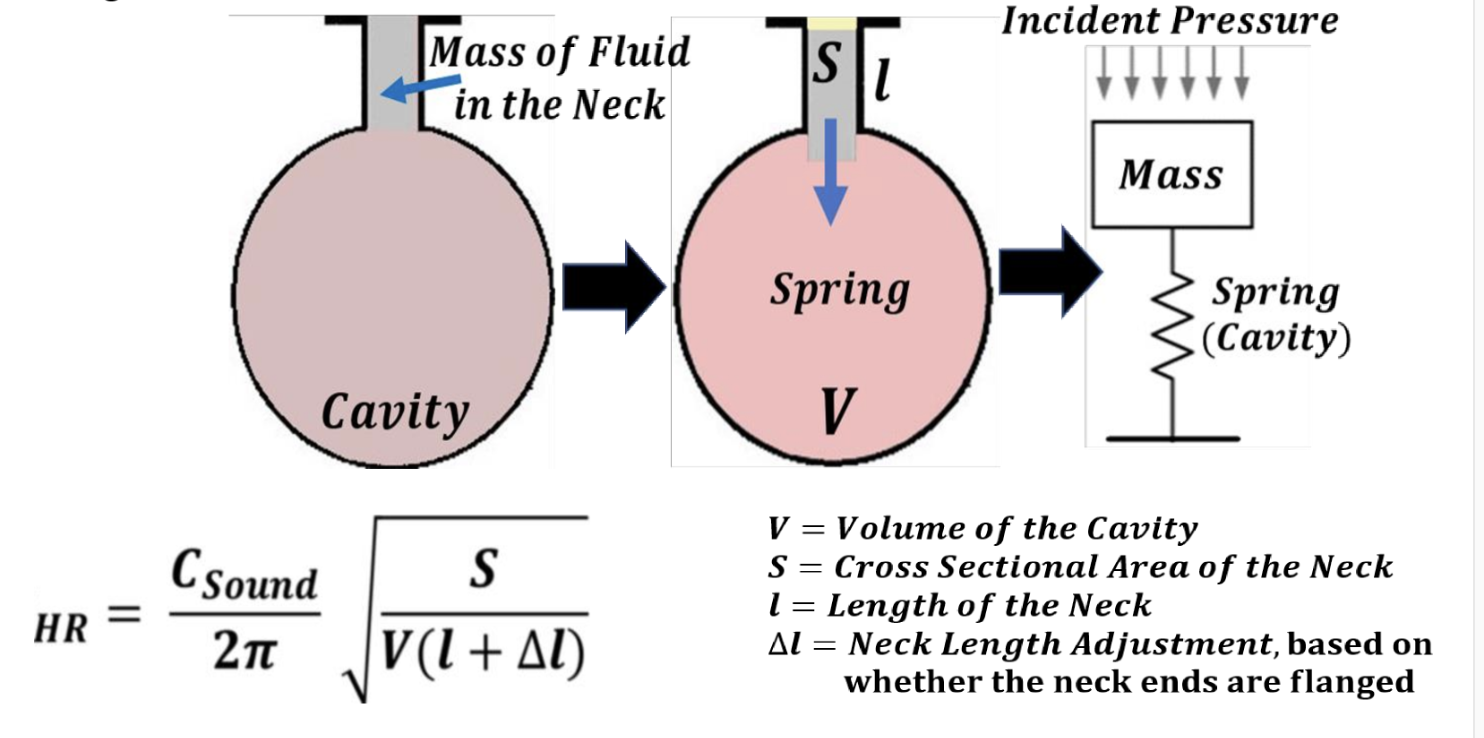
\includegraphics[width=0.8\linewidth,height=\textheight,keepaspectratio]
{images/Hill2018figure2screenshot.png}
\caption{Hill\autocite{Hill2018ResonanceFO} without permission.}\label{fig:resonator}
\end{figure}
We shall return to the question of the analysis of notes at a later stage, after
we have treated of the vibrations of strings, with the aid of which it is best
elucidated; but a very instructive experiment, due originally to Ohm and
improved by Helmholtz, may be given here.  Helmholtz\footnote{Tonempfindungen,
p. 109} took two bottles of the shape represented in the figure, one about
twice as large as the other.  These were blown by streams of air directed
across the mouth and issuing from gutta-percha tubes, whose ends had been
softened and pressed flat, so as to reduce the bore to the form of a narrow
slit, the tubes being in connection with the same bellows. By pouring in water
when the note is too low and by partially obstructing the mouth when the note
is too high, the bottles may be made to give notes with the exact interval of
an octave, such as b and b'. The larger bottle, blown alone, gives a somewhat
muffled sound similar in character to the vowel U; but, when both bottles are
blown, the character of the resulting sound is sharper, resembling rather the
vowel O. For.a short time after the notes had been heard separately Helmholtz
was able to distinguish them in the mixture; but as the memory of their
separate impressions faded, the higher note seemed by degrees to amalgamate
with the lower, which at the same time became louder and acquired a sharper
character. This blending of the two notes may take place even when the high
note is the louder.

Simple tones correspond to simple pendulous vibrations.  27. Seeing now that
notes are usually compound, and that only a particular sort called tones are
incapable of further analysis, we are led to inquire what is the physical
characteristic of tones, to which they owe their peculiarity. What sort of
periodic vibration is it, which produces a simple tone? According to what
mathematical function of the time does the pressure vary in the passage of the
ear? No question in Acoustics can be more important.

The simplest periodic functions with which mathematicians are acquainted are
the circular functions, expressed by a sine or cosine; indeed there are no
others at all approaching them in simplicity. They may be of any period, and
admitting of no other variation (except magnitude), seem well adapted to
produce simple tones. Moreover it has been proved by Fourier, that the most
general single-valued periodic function can be resolved into a series of
circular functions, having periods which are submultiples of that of the given
function. Again, it is a consequence of the general theory of vibration that
the particular type, now suggested as corresponding to a simple tone, is the
only one capable of preserving its integrity among the vicissitudes which it
may have to undergo. Any other kind is liable to a sort of physical analysis,
one part being differently affected from another. If the analysis within the
ear proceeded on a different principle from that effected according to the laws
of dead matter outside the ear, the consequence would be that a sound
originally simple might become compound on its way to the observer. There is no
reason to suppose that anything of this sort actually happens. When it is added
that according to all the ideas we can form on the subject, the analysis within
the ear must take place by means of a physical machinery, subject to the same
laws as prevail outside, it will be seen that a strong case has been made out
for regarding tones as due to vibrations expressed by circular functions. We
are not however left entirely to the guidance of general considerations like
these. In the chapter on the vibration of strings, we shall see that in many
cases theory informs us beforehand of the nature of the vibration executed by a
string, and in particular whether any specified simple vibration is a component
or not. Here we have a decisive test. It is found by experiment that, whenever
according to theory any simple vibration is present, the corresponding tone can
be heard, but, whenever the simple vibration is absent, then the tone cannot be
heard. We are therefore justified in asserting that simple tones and vibrations
of a circular type are indissolubly connected. This law was discovered by Ohm.

\chapter{Harmonic Motions}\label{harmonic-motions} % pdf page 36, LaTeX page 17

28.  Composition of harmonic motions of like period.  The vibrations expressed
by a circular function of the time and variously designated as simple,
pendulous, or harmonic, are so important in Acoustics that we cannot do better
than devote a, chapter to their consideration, before entering on the dynamical
part of our subject. The quantity, whose variation constitutes the vibration,
may be the displacement of a particle measured in a given direction, the
pressure at a fixed point in a fluid medium, and so on.  In any case denoting
it by u, we have
\begin{equation*} u =a \cos(2 \pi t/ \tau ) - \epsilon ), \tag{1}
\end{equation*}
in which a denotes the amplitude, or extreme value of
u; \(\tau\)is the periodic time, or period, after the lapse of which the values
of u recur; and \(\epsilon\) determines the phase of the vibration at the
moment from which t is measured.

Any number of harmonic vibrations of the same period affecting a variable
quantity, compound into another of the same type, whose elements are determined
as follows:
\begin{align*}
u & =\sum a \cos \left(\frac{2 \pi t}{\tau}-\epsilon\right) \\
& =\cos \frac{2 \pi t}{\tau}
\sum \left( a \cos \epsilon+\sin \frac{2 \pi t}{\tau} \Sigma a \sin \epsilon \right) \\
& =r \cos \left(\frac{2 \pi t}{\tau}-\theta\right) \tag{2}.
\end{align*}
if
\begin{equation*} r=\left\{\left(\sum a \cos \epsilon\right)^2+\left(\sum a
\sin \epsilon\right)^2\right\}^{\frac{1}{2}} . \tag{3}
\end{equation*}
and
\begin{equation*} \tan \theta=\frac{ \sum a \sin \epsilon }{\Sigma a \cos
\epsilon} \tag{4}
\end{equation*}
and

For example, let there be two components,
\[
u=a \cos \left(\frac{2 \pi t}{\tau}-\epsilon\right)+
a^{\prime} \cos \left(\frac{2 \pi t}{\tau}-\epsilon^{\prime}\right);
\]
then
\begin{equation*}
r=\left\{a^2+a^{\prime 2}+2 a a^{\prime} \cos
\left(\epsilon-\epsilon^{\prime}\right)\right\}^{\frac{1}{2}} \tag{5}
\end{equation*}
\begin{equation*} \tan \theta= \frac{a \sin \epsilon+a^{\prime}
\sin \epsilon^{\prime}}{a \cos \epsilon+a^{\prime} \cos \epsilon^{\prime}} \tag{6}.
\end{equation*}
Particular cases may be noted. If the phases of the two components agree,
\[u=\left(a+a^{\prime}\right) \cos \left(\frac{2 \pi t}{\tau}-\epsilon\right) .\]

If the phases differ by half a period,
\[u=\left(a-a^{\prime}\right) \cos
\left(\frac{2 \pi t}{\tau}-\epsilon\right),\]
so that if \(a'=a\), \(u\)
vanishes. In this case the vibrations are often said to \textit{interfere}, but
the expression is rather misleading. Two sounds may very properly be said to
interfere, when they together cause silence; but the mere superposition of two
Vibrations (whether rest is the consequence, or not) cannot properly be so
called. At least if this be interference, it is difficult to say what
non-interference can be. It will appear in the course of this work that when
vibrations exceed a certain intensity they no longer compound by mere addition;
\textit{this} mutual action might more properly be called interference, but it
is a phenomenon of a totally different nature from that with which we are now
dealing.

Again, if the phases differ by a quarter or by three-quarters of a period,
\(\cos(\epsilon- \epsilon')=0\), and
\[r= \sqrt{ a^2 +(a')^2}.\]
Harmonic vibrations of given period may be represented by lines drawn from a pole, the
lengths of the lines being proportional to the amplitudes, and the inclinations
to the phases of the vibrations. The resultant of any number of harmonic
vibrations is then represented by the geometrical resultant of the
corresponding lines. For example, if they are disposed symmetrically round the
pole, the resultant of the lines, or vibrations, is zero.
\begin{figure}[htbp]
% pdf page 34 \centering
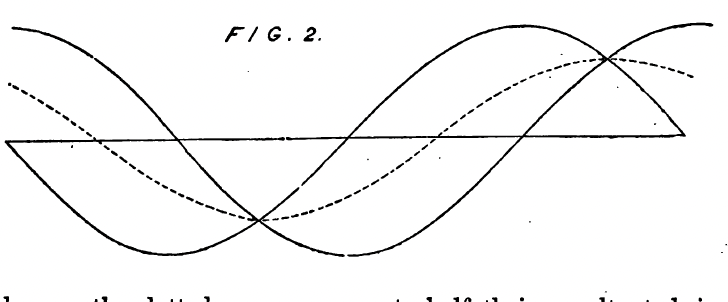
\includegraphics[width=0.8\linewidth,height=\textheight,keepaspectratio]{images/figure2.png}
\caption{Two harmonic curves of the same wave-length and amplitude have
different phases; the dotted curve represents half their resultant, being the
locus of points midway between those in which the two curves are met by any
ordinate.}\label{fig:superposition}
\end{figure}

29.  Harmonic Curve.  If we measure off along an axis of x distances
proportional to the time, and take w for an ordinate, we obtain the harmonic
curve, or curve of sines,
\[ u=a \cos \left(\frac{2 \pi xt}{\lambda}-\epsilon\right), \]
where \(\lambda\), called the wave-length, is
written in place of \(\tau \), both quantities denoting the range of the
independent variable corresponding to a complete recurrence of the function.
The harmonic curve is thus the locus of a point subject at once to a uniform
motion, and to a harmonic vibration in a perpendicular direction. In the next
chapter we shall see that the vibration of a tuning fork is simple harmonic; so
that if an excited tuning fork is moved with uniform velocity parallel to the
line of its handle, a tracing point attached to the end of one of its prongs
describes a harmonic curve, which may be obtained in a permanent form by
allowing the tracing point to bear gently on a piece of smoked paper.


30.  Beats.  If two harmonic vibrations of different periods coexist,
\[
u= a \cos \left(\frac{2 \pi t}{\tau}-\epsilon\right)-
a^{\prime} \cos \left(\frac{2 \pi t}{\tau^{\prime}}-\epsilon^{\prime}\right).
\]
The resultant cannot here
be represented as a simple harmonic motion with other elements.  If \(\tau \)
and \( \tau^{\prime}\) be incommensurable, the value of \(u\) never recurs;
but, if \( \tau \) and \( \tau^{\prime} \) be in the ratio of two whole
numbers, \(u\) recurs after the lapse of a time equal to the east common
multiple of \( \tau \) and \( \tau^{\prime} \); but the vibration is not simple
harmonic.  For example, when a note and its fifth are sounding together, the
vibration recurs after a time equal to twice the period of the graver.

One case of the composition of harmonic vibrations of different periods is
worth special discussion, namely, when the difference of the periods is small.
If we fix our attention on the course of things during an interval of time
including merely a few periods, we see that the two vibrations are nearly the
same as if their periods were absolutely equal, in which case they would, as we
know, be equivalent to another simple harmonic vibration of the same period.
For a few periods then the resultant motion is approximately simple harmonic,
but the same harmonic will not continue to represent it for long. The vibration
having the shorter period continually gains on its fellow, thereby altering the
difference of phase on which the elements of the resultant depend. For
simplicity of statement let us suppose that the two components have equal
amplitudes, frequencies represented by \(m\) and \(n\), where m-n is small, and
that when first observed their phases agree.  At this moment their effects
conspire, and the resultant has an amplitude double of that of the components.
But after a time
\[ \frac{1}{ 2(m-n) } \]
the vibration m will have gained half
a period relatively to the other;.and the two, being now in complete
disagreement, neutralize each other. After a further interval of time equal to
that above named, m will have gained altogether a whole vibration, and complete
accordance is once more re-established. The resultant motion is therefore
approximately simple harmonic, with an amplitude not constant, but varying from
zero to twice that of the components, the frequency of these alterations being
m-n. If two tuning forks with frequencies 500 and 501 be equally excited, there
is every second a rise and fall of sound corresponding to the coincidence or
opposition of their vibrations.

This phenomenon is called beats. We do not here fully discuss the question how
the ear behaves in the presence of vibrations having nearly equal frequencies,
but it is obvious that if the motion in the neighbourhood of the ear almost
ceases for a considerable fraction of a second, the sound must appear to fall.
For reasons that will afterwards appear, beats are best heard when the
interfering sounds are simple tones. Consecutive notes of the stopped diapason
of the organ shew the phenomenon very well, at least in the lower parts of the
scale. A permanent interference of two notes may be obtained by mounting two
stopped organ pipes of similar construction and identical pitch side by side on
the same wind chest. The vibrations of the two pipes adjust themselves to
complete opposition, so that at a little distance nothing can be heard, except
the hissing of the wind. If by a rigid wall between the two pipes one sound
could be cut off, the other would be instantly restored. Or the balance, on
which silence depends, may be upset by connecting, the ear with a tube, whose
other end lies close to the mouth of one of the pipes.

By means of beats two notes may be tuned to unison with great exactness.  The
object is to make the beats as slow as possible, since the number of beats in a
second is equal to the difference of the frequencies of the notes. Under
favourable circumstances beats so slow as one in 30 seconds may be recognised,
and would indicate that the higher note gains only two vibrations a minute on
the lower. Or it might be desired merely to ascertain the difference of the
frequencies of two notes nearly in unison, in which case nothing more is
necessary than to count the number of beats. It will be remembered that the
difference of frequencies does not determine the interval between the two
notes; that depends on the ratio of frequencies. Thus the rapidity of the beats
given by two notes nearly in unison is doubled, when both are taken an exact
octave higher.

% pdf page 40
Analytically
\[u=a \cos (2 \pi m t-\epsilon)+a^{\prime} \cos \left(2 \pi n t-\epsilon^{\prime}\right),\]
where \(m-n\) is small. Now
\(\cos \left(2 \pi n t-\epsilon^{\prime}\right)\)
may be written
\[\cos \left\{2 \pi m t-2 \pi(m-n) t-\epsilon^{\prime}\right\},\]
and we have
\[u=r \cos (2 \pi m t-\theta) \tag{1}, \]
where
\[
r^2=a^2+a^{\prime 2}+2 a a^{\prime} \cos \left\{2 \pi(m-n)
t+\epsilon^{\prime}-\epsilon\right\} \tag{2},
\]
\[
\tan \theta=
\frac{a \sin \epsilon+a^{\prime} \sin \left\{2 \pi(m-n) t+\epsilon^{\prime}\right\}}
{a \cos \epsilon+a^{\prime} \cos \left\{2 \pi(m-n) t+\epsilon^{\prime}\right\}} \tag{3}.
\]
The resultant vibration may thus be considered as harmonic with
elements \(r\) and \(\theta\), which are not constant but slowly varying
functions of the time, having the frequency \(m-n\).  The amplitude \(r\) is at
its maximum when
\[\cos \left\{2 \pi(m-n)
t+\epsilon^{\prime}-\epsilon\right\}=+1,\]
and at its minimum when
\[\cos \left\{2 \pi(m-n) t+\epsilon^{\prime}-\epsilon\right\}=-1,\]
the corresponding
values being \(a+a^{\prime}\) and \(a-a^{\prime}\) respectively.

31.  Fourier's Theorem. Another case of great importance is the composition of
vibrations corresponding to a tone and its harmonics, It is known that the most
general single-valued finite periodic function can be expressed by a series of
simple harmonics
\[ u=a_0+\sum_{n \geq 1} a_n \cos \left(\frac{2 \pi n t}{\tau}-\epsilon_n\right) \tag{1},\]
a theorem usually quoted as Fourier's.
Analytical proofs will be found in Todhunter's \textit{Integral Calculus} and
Thomson and Tait's \textit{Natural Philosophy}; and a line of argument almost
if not quite amounting to a demonstration will be given later in this work. A
few remarks are all that will be required here.

Fourier's theorem is not obvious. A vague notion is not uncommon that the
infinitude of arbitrary constants in the series of necessity endows it with the
capacity of representing an arbitrary periodic function.  That this is an error
will be apparent, when it is observed that the same argument would apply
equally, if one term of the series were omitted; in which case the expansion
would not in general be possible.

Another point worth notice is that simple harmonics are not the only functions,
in a series of which it is possible to expand one arbitrarily given. Instead of
the simple elementary term
\[\cos \left(\frac{2 \pi n t}{\tau}-\epsilon_n\right),\]
we might take
\[
\cos \left(\frac{2 \pi n t}{\tau}-\epsilon_n\right)+
\frac{1}{2} \cos \left(\frac{4 \pi n t}{\tau}-\epsilon_n\right),
\]
formed by adding a similar one in the same phase
of half the amplitude and period. It is evident that these terms would serve as
well as the others; for
\begin{align*}
\cos \left(\frac{2 \pi n t}{\tau}-\epsilon_n\right) &
= \cos \left(\frac{2 \pi n t}{\tau}-\epsilon_n\right)+
  \frac{1}{2} \cos \left(\frac{4 \pi n t}{\tau}-\epsilon_n\right) \\
- & \frac{1}{2}\left\{
       \cos \left(\frac{4\pi nt}{\tau}-\epsilon_n\right)+
  \frac{1}{2} \cos \left(\frac{8\pi nt}{\tau}-\epsilon_n\right)
        \right\} \\
+ & \frac{1}{4}\left\{\cos \left(\frac{8\pi nt}{\tau}-\epsilon_n\right)+
     \frac{1}{2} \cos \left(\frac{16\pi nt}{\tau}-\epsilon_n\right)\right\} \\
- & \ldots \\
\end{align*}
so that each term in Fourier's series,
and therefore the sum of the series, can be expressed by means of the double
elementary terms now suggested. This is mentioned here, because students, not
being acquainted with other expansions, may imagine that simple harmonic
functions are by nature the only ones qualified to be the elements in the
development of a periodic function. The reason of the preeminent importance of
Fourier's series in Acoustics is the mechanical one referred to in the
preceding chapter, and to be explained more fully hereafter, namely, that, in
general, simple harmonic vibrations are the only kind that are propagated
through a vibrating system without suffering decomposition.

32.  Vibrations in perpendicular directions. As in other cases of a similar
character, e.g. Taylor's theorem, if the possibility of the expansion be known,
the coefficients may be determined by a comparatively simple process. We may
write (1) of
\[
u=A_0+\sum_{n\geq 1} A_n \cos \frac{2 n \pi t}{\tau}+
\sum_{n\geq 1} B_n \sin \frac{2 n \pi t}{\tau} \tag{1}.
\]
Multiplying by \(\cos \frac{2 n \pi t}{\tau}\) or
\(\sin \frac{2 n \pi t}{\tau}\), and integrating over a complete period \([0,\tau]\),
we find
\[
\left.\begin{array}{l} A_n=\frac{2}{\tau} \int_0^\tau u \cos \frac{2 n \pi t}{\tau} d t \\
B_n=\frac{2}{\tau} \int_0^\tau u \sin \frac{2 n \pi t}{\tau} d t
\end{array}\right\} \tag{2}
\]
An immediate integration gives
\[A_0=\frac{1}{\tau} \int_0^\tau u d t \tag{3} \]
indicating that \(A_o\) is
the \textit{mean} value of \(u\) throughout the period.

The degree of convergence in the expansion of depends in general on the
continuity of the function and its derivatives. The series formed by successive
differentiations of (1) converge less and less rapidly, but still remain
convergent, and arithmetical representatives of the differential coefficients
of u, so long as these latter are everywhere finite. Thus (Thomson and Tait, \S
77), if all the derivatives up to the m inclusive are free from infinite
values, the series for u is more convergent than one with for coefficients.

\section{Beats of approximate consonances}
32 a.  The general explanation of the beats beard when two pure tones nearly in
union are sounded simultaneously has been discussed in § 80. But the occurrence
of beats is not confined to the case of approximate unison, at least when we
have to deal with compound notes. Suppose for example that the interval is an
octave. The graver note then usually includes a tone coincident in pitch with
the fundamental tone of the higher note.

If the interval be disturbed, the previously coincident tones separate
from one another, and give rise to beats of the same frequency as if
they existed alone. There is usually no difficulty in observing these
beats; but if one or both of the component tones concerned be very
faint, the aid of a resonator may be invoked.

In general we may consider that each consonant interval is characterized
by the coincidence of certain component tones, and if the interval be
disturbed the previously coincident tones give rise to beats. Of course
it may happen in any particular case that the tones which would coincide in
pitch are absent from one or other of the notes. The disturbance of the
interval would then, according to the above theory, not be attended by beats.
In practice faint beats are usually heard; but the discussion of this
phenomenon, as to which authorities are not entirely agreed, must be postponed.

33. Consonant intervals. Another class of compounded vibrations, interesting
from the facility with which they lend themselves to optical observation, occur
when two harmonic vibrations affecting the same particle are executed in
perpendicular directions, more especially when the periods are not only
commensurable, but in the ratio of two small whole numbers. The motion is then
completely periodic, with a period not many times greater than those of the
components, and the curve described is re-entrant. If w and v be the
coordinates, we may take
\[u=a \cos(2rnt-\epsilon), \quad v=b \cos(Qrm t) (1).\]
First let us suppose that the periods are equal, so that n'=n; the elimination
of t ges for the equation of the curve described,
\[\frac{u^2}{a^2}+\frac{v^2}{b^2}-\frac{2uv}{ab}\cos(\epsilon)-\sin^2(\epsilon)=0,\]
(2) representing in general an ellipse, whose position and dimensions depend
upon the amplitudes of the original vibrations and upon the difference of their
phases. If the phases differ by a quarter period, \(\cos(e)=0\), and the equation becomes
\[ \frac{u^2}{a^2} +  \frac{v^2}{b^2} =1.  \]

In this case the axes of the ellipse coincide with those of coordinates, If
further the two components have equal amplitudes, the locus degenerates into
the circle
\[ u^2 +  v^2 = a^2,\]
which is described with uniform velocity.
This shews how a uniform circular motion may be analysed into two rectilinear
harmonic motions, whose directions are perpendicular.

If the phases of the components agree, \(\epsilon = 0\), and the ellipse
degenerates into the coincident straight lines
\[ \left( \frac{u}{a} - \frac{v}{b}\right)^2 = 0 \]
if the difference of phase amount to half a period,
\[ \left( \frac{u}{a} + \frac{v}{b}\right)^2 = 0 \]

When the unison of the two vibrations is exact, the elliptic path remains
perfectly steady, but in practice it will almost always happen that there is a
slight difference between the periods. The consequence is that though a fixed
ellipse represents the curve described with sufficient accuracy for a few
periods, the ellipse itself gradually changes in correspondence with the
alteration in the magnitude of . It becomes therefore a matter of interest to
consider the system of ellipses represented by (2), supposing a and b
constants, but e variable.

Since the extreme values of u and v are +a, +b respectively, the ellipse is in
all cases inscribed in the rectangle whose sides' are 2a, 2b.  Starting with
the phases in agreement, or e=0, we have the ellipse coincident with the
diagonal F =0. As e increases from 0 to 7, the ellipse opens out until its equation becomes

From this point it closes up again, ultimately coinciding with the other
diagonal - + = 0, corresponding to the increase of e from 3a to m.  After this,
as e ranges from a to 27, the ellipse retraces its course until it again
coincides with the first diagonal. The sequence of changes is exhibited in Fig.  3,

FIG.3.

The ellipse, having already four given tangents, is completely determined by
its point of contact P (Fig. 4) with the line v=d.

In order to connect this with \(\epsilon\), e, it is sufficient to observe that
when \(v=b\), \(\cos(2 \pi nt) =1\); and therefore \(u=a \cos(\epsilon)\). Now
if the elliptic paths be the result of the superposition of two harmonic
vibrations of nearly coincident pitch, \(\epsilon\) varies uniformly with the
time, so that P itself executes a harmonic vibration along AA' with a frequency
equal to the difference of the two given frequencies.

34.  Lissajous’ Cylinder. Lissajous\footnote{Annales de Chimie (3) LI  147}
has shewn that this system of ellipses may be regarded as the different aspects
of one and the same ellipse described on the surface of a transparent cylinder.
In Fig. 5 A A' B' B represents the cylinder, of which AB' is a plane section.
Seen from an infinite distance in the direction of the common tangent at A to
the plane sections, the cylinder is projected into a rectangle, and the ellipse
into its diagonal. Suppose now that the cylinder turns upon its axis, carrying
the plane section with it. Its own projection remains a constant rectangle in
which the projection of the ellipse is inscribed. Fig. 6 represents the
position of the cylinder after a rotation through a right angle. It appears
therefore that by turning the cylinder round we obtain in succession all the
ellipses corresponding to the paths described by a point subject to two
harmonic vibrations of equal period and fixed amplitudes. Moreover if the
cylinder be turned continuously with uniform velocity, which insures a harmonic
motion for P, we obtain a complete representation of the varying orbit
described by the point when the periods of the two components differ slightly,
each complete revolution answering to a gain or loss of a single vibration
\footnote{By a vibration will always be meant in this work a complete cycle of
changes}. The revolutions of the cylinder are thus synchronous with the beats
which would result from the composition of the two vibrations, if they were to
act in the same direction.

FIG. 5.  FIG. 6.

35. Lissajous' Figures. Vibrations of the kind here considered are very easily
realized experimentally. A heavy pendulum-bob, hung from a fixed point by a
long wire or string, describes ellipses under the action of gravity, which may
in particular cases, according to the circumstances of projection, pass into
straight lines or circles. But in order to see the orbits to the best
advantage, it is necessary that they should be described so quickly that the
impression on the retina made by the moving point at any part of its course has
not time to fade materially, before the point comes round again to renew its
action. This condition is fulfilled by the vibration of a silvered bead (giving
by reflection a luminous point), which is attached to a straight metallic wire
(such as a knitting-needle), firmly clamped in a vice at the lower end.  When
the system is set into vibration, the luminous point describes ellipses, which
appear as fine lines of light. These ellipses would gradually contract in
dimensions under the influence of friction until they subsided into a
stationary bright point, without undergoing any other change, were it not that
in all probability, owing to some want of symmetry, the wire has slightly
differing periods according to the plane in which the vibration is executed.
Under these circumstances the orbit is seen to undergo the cycle of changes
already explained.

36. Optical methods of composition and analysis. So far we have supposed the
periods of the component vibrations to be equal, or nearly equal; the next case
in order of simplicity is when one is the double of the other. We have
\[u=a \cos(4n \pi t-\epsilon), \quad v= b \cos(2n \pi t).\]
The locus resulting from the elimination of \(t\) may be written
\[
\frac{u}{a} = \left( 2 \frac{v^2}{b^2} -1 \right) \cos (\epsilon ) +
\frac{2v}{b} \sqrt{1-\frac{v^2}{b^2}} ~~ \sin(\epsilon),
\]
(1) which for all values of \(\epsilon\) represents a curve inscribed in the
rectangle 2a, 2b.  \todo[inline]{ exponent of 2nd v smudged in text} If e=0, or
7, we have

o u 2 - a) (1 + i), representing parabolas, Fig. 7 shews the various curves for
the intervals of the octave, twelfth, and fifth.

\todo[inline]{Z is a sigma for summation} FIG C Z

To all these systems Lissajous' method of representation by the transparent
cylinder is applicable, and when the relative phase is altered, whether from
the different circumstances of projection in different cases, or continuously
owing to a slight deviation from exactness in the ratio of the periods, the
cylinder will appear to turn, so as to present to the eye different aspects of
the same line traced on its surface.

37.  Blackburn's pendulum.  There is no difficulty in arranging a vibrating
system so that the motion of a point shall consist of two harmonic vibrations
in perpendicular planes, with their periods in any assigned ratio, The simplest
is that known as Blackburn's pendulum. A wire ACB is fastened at A and B, two
fixed points at the same level, The bob P is attached to its middle point by
another wire CP. For vibrations in the plane of the diagram, the point of
suspension is practically C, provided that the wires are sufficiently
stretched; but for a motion perpendicular to this plane, the bob turns about D,
carrying the wire 4 OB with it. The periods of vibration in

A; 0 : B

the principal planes are in the ratio of the square roots of CP and DP.  Thus
if DC=3CP, the bob describes the figures of: the octave. To obtain the sequence
of curves corresponding to approximate unison ACB must be so nearly tight, that
CD is relatively small.

38.  Kaleidophone.  Another contrivance called the kaleidophone was originally
invented by Wheatstone. A straight thin bar of steel carrying a bead at its
upper end is fastened in a vice, as explained in a previous paragraph. If the
section of the bar is square, or circular, the period of vibration is
independent of the plane in which it is performed. But let us suppose that the
section is a rectangle with unequal sides. The stiffness of the bar --the force
with which it resists bending-- is then greater in the plane of greater
thickness, and the vibrations in this plane have the shorter period.  By a
suitable adjustment of the thicknesses, the two periods of vibration may be
brought into any required ratio, and the corresponding curve exhibited.

The defect in this arrangement is that the same bar will give only one set of
figures. In order to overcome this objection the following modification has
been devised. A slip of steel is taken whose rectangular section is very
elongated, so that as regards bending in one plane the stiffness is so great as
to amount practically to rigidity.  The bar is divided into two parts, and the
broken ends reunited, the two pieces being turned on one another through a
right angle, so that the plane, which contains the small thickness of one,
contains the great thickness of the ether. When the compound rod is clamped in
a vice at a point below the junction, the period of the vibration in one
direction, depending almost entirely on the length of the upper piece, is
nearly constant; but that in the second direction may be controlled by varying
the point at which the lower piece is clamped.

39. In this arrangement the luminous point itself executes the vibrations which
are to be observed; but in Lissajous' form of the experiment, the point of
light remains really fixed, while its image is thrown into apparent motion by
means of successive reflection from two vibrating mirrors. A small hole in an
opaque screen placed close to the flame of a lamp gives a point of light, which
is observed after reflection in the mirrors by means of a small telescope. The
mirrors, usually of polished steel, are attached to the prongs of stout tuning
forks, and the whole is so disposed that when the forks are thrown into
vibration the luminous point appears to describe harmonic motions in
perpendicular directions, owing to the angular motions of the reflecting
surfaces. The amplitudes and periods of these harmonic motions depend upon
those of the corresponding forks, and may be made such as to give with enhanced
brilliancy any of the figures possible with the kaleidophone. By a similar
arrangement it is possible to project the figures on a screen. In either case
they gradually contract as the vibrations of the forks die away.

40. The principles of this chapter have received an important application in
the investigation of rectilinear periodic motions. When a point, for instance a
particle of a sounding string, is vibrating with such a period as to give a
note within the limits of hearing, its motion is much too rapid to be followed
by the eye; so that, if it be required to know the character of the vibration,
some indirect method must be adopted. The simplest, theoretically, is to
compound the vibration under examination with a uniform motion of translation
in a perpendicular direction, as when a tuning fork draws a harmonic curve on
smoked paper.  Instead of moving the vibrating body itself, we may make use of
a revolving mirror, which provides us with an image in motion. In this way we
obtain a representation of the function characteristic of the vibration, with
the abscissa proportional to time.

But it often happens that the application of this method would be difficult or
inconvenient. In such cases we may substitute for the uniform motion a harmonic
vibration of suitable period in the same direction. To fix our ideas, let us
suppose that the point, whose motion we wish to investigate, vibrates
vertically with a period 7, and let us examine the result of combining with
this a horizontal harmonic motion, whose period is some multiple of 1, say, nr.
Take a rectangular piece of paper, and with axes parallel to its edges draw the
curve representing the vertical motion (by setting off abscissa proportional to
the time) on such a scale that the paper just contains repetitions or waves,
and then bend the paper round so as to form a cylinder, with a re-entrant curve
running round it. A point describing this curve in such a manner that it
revolves uniformly about the axis of the cylinder will appear from a distance
to combine the given vertical motion of period 7, with a horizontal harmonic
motion of period nr. Conversely therefore, in order to obtain the
representative curve of the vertical vibrations, the cylinder containing the
apparent path must be imagined to be divided along a generating line, and
developed into a plane. There is less difficulty in conceiving the cylinder and
the situation of the curve upon it, when the adjustment of the periods is not
quite exact, for then the cylinder appears to turn, and the contrary motions
serve to distinguish those parts of the curve which lie on its nearer and
further face.

41. The vibration microscope.  The auxiliary harmonic motion is generally
obtained optically, by means of an instrument called a vibration-microscope
invented by Lissajous. One prong of a large tuning fork carries a lens, whose
axis is perpendicular to the direction of vibration; and which may be used
either by itself, or as the object-glass of a compound microscope formed by the
addition of an eye-piece independently supported. In either case a stationary
point is thrown into apparent harmonic motion along a line parallel to that of
the fork's vibration.

The vibration-microscope may be applied to test the rigour and universality of
the law connecting pitch and period. Thus it will be found that any point of a
vibrating body which gives a pure musical note will appear to describe a
re-entrant curve, when examined with a vibration-microscope whose note is in
strict unison with its own. By the same means the ratios of frequencies
characteristic of the consonant intervals may be verified; though for this
latter purpose a more thoroughly acoustical method, to be described in a future
chapter, may be preferred.

42. Intermittent illumination.  Another method of examining the motion of a
vibrating body depends upon the use of intermittent illumination
\footnote{Plateau, Bull. de l'Aca. roy. de Belgique, t. III, p. 364, 1836}.
Suppose, for example, that by means of suitable apparatus a series of electric
sparks are obtained at regular intervals \(\tau\).  A vibrating body, whose
period is also \(\tau\), examined by the light of the sparks must appear at
rest, because it can be seen only in one position. If, however, the period of
the vibration differ from \(\tau\) ever so little, the illuminated position
varies, and the body will appear to vibrate slowly with a frequency which is
the difference of that of the spark and that of the body. The type of vibration
can then be observed with facility.

The series of sparks can be obtained from an induction-coil, whose primary
circuit is periodically broken by a vibrating fork, or by some other
interrupter of sufficient regularity. But a better result is afforded by
sunlight rendered intermittent with the aid of a fork, whose prongs carry two
small plates of metal, parallel to the plane of vibration and close together.
In each plate is a slit parallel to the prongs of the fork, and so placed as to
afford a free passage through the plates when the fork is at rest, or passing
through the middle point of its vibrations. On the opening so formed, a beam of
sunlight is concentrated by means of a burning glass, and the object under
examination is placed in the cone of rays diverging on the further side
\footnote{Topler, Phil. Mag. Jan. 1867.}.  When the fork is made to vibrate by
an electromagnetic arrangement, the illumination is cut off except when the
fork is passing through its position of equilibrium, or nearly so. The flashes
of light obtained by this method are not so instantaneous as electric sparks
(especially when a jar is connected with the secondary wire of the coil), but
in my experience the regularity is more perfect. Care should be taken to cut
off extraneous light as far as possible, and the effect is then very striking.

A similar result may be arrived at by looking at the vibrating body through a
series of holes arranged in a circle on a revolving disc.  Several series of
holes may be provided on the same disc, but the observation is not satisfactory
without some provision for securing uniform rotation.

Except with respect to the sharpness of definition, the result is the same when
the period of the light is any multiple of that of the vibrating body. This
point must be attended to when the revolving wheel is used to determine an
unknown frequency.

When the frequency of intermittence is an exact multiple of that of the
vibration, the object is seen without apparent motion, but generally in more
than one position. This condition of things is sometimes advantageous.

Similar effects arise when the frequencies of the vibrations and of the flashes
are in the ratio of two small whole numbers. If, for example, the number of
vibrations in a given time be half as great again as the number of flashes, the
body will appear stationary, and in general double.

\section{Random phases.}
42 a.  We have seen (§ 28) that the resultant of two isoperiodic vibrations of equal
amplitude is wholly dependent upon their phase relation, and it is of interest
to inquire what we are to expect from the composition of a large number \(n\)
of equal vibrations of amplitude unity, of the same period, and of phases
accidentally determined. The intensity of the resultant, represented by the
square of the amplitude § 245, \todo[inline]{volume 2 article245?} will of
course depend upon the precise manner in "which the phases are distributed, and
may vary from \(n^2\) to zero. But is there a definite intensity which becomes
more and more probable when \(n\) is increased without limit?

The nature of the question here raised is well illustrated by the special case
in which the possible phases are restricted to two opposite phases. We may then
conveniently discard the idea of phase, and regard the amplitudes as at random
positive or negative. If all the signs be the same, the intensity is \(n^2\);
if, on the other hand, there be as many positive as negative, the result is
zero. But although the intensity may range from 0 to \(n^2\), the smaller
values are more probable than the greater.

The simplest part of the problem relates to what is called in the theory of
probabilities the \textit{expectation} of intensity, that is, the mean
intensity to be expected after a great number of trials, in each of which the
phases are taken at random. The chance that all the vibrations are positive is
\(2^{-n}\) and thus the expectation of intensity corresponding to this
contingency is \(2^{-n} n^2\).  In like manner the expectation corresponding to
the number of positive vibrations being \(n-1\) is
\[2^{-n} n (n-2)^2,\]
and so on. The whole expectation of intensity is thus
\[
2^{-n} \left( \begin{pmatrix} n \\ 0 \end{pmatrix} n^2 +
\begin{pmatrix} n \\ 1\\ \end{pmatrix} (n-2)^2 +
\begin{pmatrix} n \\ 2\\ \end{pmatrix} (n-4)^2 + \ldots \right) =
\]
\[ 2^{-n} \sum_{k=0}^n \begin{pmatrix} n \\ k \end{pmatrix} (n-2k)^2. \]
(1) Now the sum of the (n + 1) terms of this series is simply \(n\), as may be
proved by comparison of coefficients of \(x^2\) in the equivalent forms

The expectation of intensity is therefore \(n\), and this whether \(n\), be great or small.

The same conclusion holds good when the phases are unrestricted. From (3) § 28,
if \(a_1 = a_2 = \ldots = 1\),
\[
r^2 = (cos \epsilon_1 + cos \epsilon_2 + \ldots)^2 +
      (sin \epsilon_1 + sin \epsilon_2 + \ldots)^2
\]
\[ n + 2 \sum cos ( \epsilon_2 - \epsilon_1 ) \]
(2), where under the sign of summation are to be included the cosines
of the \(n(n-1)/2\) differences of phase. When the phases are
accidentally the sum is as likely to be positive as negative;
and thus the mean value of
\(r^2\)
is
\(n\).

The reader must be on his guard here against a fallacy, which has misled
some eminent authors. We have nut proved that when n is large there is
any tendency for a single combination to give an intensity equal to n,
but the quite different proposition that in a large number of trials, in
e h of which the phases are distributed at random, the mean intensity
will tend more and more to the value n. It is true that even in a single
combination there is no reason why any of the cosines in (2) should be
positive rather than negative. From this we may infer that when n is
increased the sum of the terms tends to vanish in comparison with the number of
terms; but, the number of the terms being of the order n we can infer nothing
as to the value of the sum of the series in comparison with n.

So far there is no difficulty; but a complete investigation of this
subject involves an estimate of the relative probabilities of resultants
lying within assigned limits of magnitude. For example, we ought to be
able to say what is the probability that the intensity due to a large
number (re) of equal components is less than n. This problem may
conveniently be considered here, though it is naturally beyond the reach
of elementary methods. We will commence by taking it under the
restriction that the phases are of two opposite kinds only.

Adopting the statistical method of statement, let us suppose that there
are an immense number N of independent combinations, each consisting of
n unit vibrations, positive or negative, and combined accidentally. When
N is sufficiently large, the statistics become regular; and the number
of combinations in which the resultant amplitude is found equal to x may
be denoted by
\( N f(n, x)\), where
\(f\) is a definite function of
\(n\) and \(x\). Now suppose that each of the N
combinations receives another random contribution of ± 1, and inquire
how many of them will subsequently possess a resultant x. It is clear
that those only can do so which originally had amplitudes x-1 or x+1.
Half of the former, and half of the latter number will acquire the
amplitude x,
so that the number required is
\[ \frac{1}{2} Nf(n, x-1) + \frac{1}{2} Nf(n,x+1).\]
But this must be identical with the number corresponding to
\(n + 1\) and \(x\), so that
\[f(n+1, x)=\frac{1}{2} f(n,x-1) + \frac{1}{2} f(n,x+1).\]
(3) This equation of differences holds good for all integral values of a and
for all positive integral values of n. If f(n, a) he given for one value
of n, the equation suffices to determine (n, x) for all higher integral
values of n. For the present purpose the initial value of a is zero. In
that case we know that for
all values of x other than zero, and that when x = 0,(0, 0) = 1.

The problem proposed in the above form is perfectly definite ; but for
our immediate object it suffices to limit ourselves to the supposition
that n is great, regarding (a, d) as a continuous function of continuous
variables n and x, much as in the analogous problem of §§ 120, 121, 122.

Writing (3) in the form
\[f(n+1,x)-f(n,x)=\frac{1}{2} f(n,x-1) + \frac{1}{2} f(n,x+1) -f(n,x),\]
(4) we see that the left-hand member may then be identified with
\( df/dn\), and
the right-hand member with
\todo[inline]{I am not typing the correct equation}
\( df/dn\),
so that under
these circumstances the differential equation to which (3) reduces is of
the well-known form
\[ df/dn = df/dn.\]
(5)

The analogy with the conduction of heat is indeed very close; and the methods
developed by Fourier for the solution of problems in the latter subject are at
once applicable. The special condition here is that initially, that is when \(n
= 0\), \(f\) must vanish for all values of x other than zero. As may be
verified by differentiation, the special solution of (5) is then

(6)
in which is an \(A\) is an arbitrary constant to he determined from the
consideration that the whole number of combinations is \(N\).  Thus if \(dx\)
be large in comparison with unity, the number of combinations which have
amplitudes between \(x\) and \(x + dx\) is

while

so that in virtue of the known equality

\[ A \sqrt{2 \pi} = 1.\]

The final result for the number of combinations which have amplitudes between
\(x\) and \(x + dx\) is accordingly

The mean intensity is expressed by

as before.

We will now pass on to the more important problem in which the phases of
the n unit vibrations are distributed at random over the entire period.
In each combination the resultant amplitude is denoted by \(r\) and the
phase (referred to a given epoch) by
\(\theta \)
; and rectangular coordinates are taken so that
\[ x =r \cos \theta, y =r \sin \theta.\]
Thus any point (x, y) in the plane of reference represents a vibration
of amplitude \(r\) and phase
\(\theta \)
, and the whole system of
\(N\)
vibrations is
represented by a distribution of points, whose density it is our object
to determine. Since no particular phase can be singled out for
distinction, we know beforehand that the density of distribution will be
independent of \(\theta \).

Of the infinite number N of points we suppose that
\[
Nf n, X, y) dxdy
\]
are to be found within the infinitesimal area dxdy, and we will inquire as
before how this number would be changed by the addition to the n
component vibrations of one more unit vibration of accidental phase. Any
vibration which after the addition is represented by the point x, y must
before have corresponded to the point
\[ x' = x \cos \phi, y' = y' - \sin \phi.\]
where
\(\phi \)
represents the phase of the additional unit vibration. And, if for the
moment be regarded as given, to the area dxdy corresponds an equal area
\( dx' dy' \). Again, all values of
\(\phi \)
being equally probable, the factor necessary
under this head is
\(d \phi/(2 \pi) \).
Accordingly the whole number to be found in dx dy
after the superposition of the additional unit is

Ndxdy;

and this is to be equated to

Ndxdyf(n + 1, x, y);

so  that
f(n + 1, x, y) = (8).

The value of f (n, x', y') is
obtained by introduction of the values of x', y' and expansion:

( '. y') (
. y) - + 5 cos sin + 5 y sin B +

so that

( y') 2ir = ( y) + i

Also, n being very great,

f(n + 1, x, y) -f (n, x, y) = df/dn ;

and (8) reduces to
(9)
the usual equation for the conduction of heat in two dimensions.

In addition to (9), f has to satisfy the special condition of evanescence
when n 0 for all points other than the origin. The appropriate solution
is necessarily symmetrical round the origin, and takes the form (n, X,
y) = (10),

as may be verified by differentiation. The constant A is to
be determined by the condition that the whole number is N, Thus N = NArr
j dxdy NA 27ri J e rdr irAN

and the number of vibrations within the
area dxdy becomes e-w+ rfar(iM (11). ini

If we wish to find the number of vibrations which have amplitudes between \(r\) and
\(r+dr\),
 we must introduce polar coordinates and integrate with respect to
0.
The required number is thus \footnote{Phil. Mag. Aug. 1880.} (12)

The result may also be expressed by saying that the probability
of a resultant amplitude between \(r\) and \(r+dr\) when a large
number n of unit vibrations are compounded at random is

rr e- i rdr (13).

The mean intensity is given by 2n''\,' I = Jo as was to be expected. The
probability of a resultant amplitude less than \(r\) is J er rdr = 1 - (14),
or, which is the same thing, the probability of a resultant amplitude
greater than \(r\) is (15). The following table gives the probabilities of
intensities less than the fractions of n named in the first column. For
example, the probability of intensity less than n is 6321.
\begin{table}[h]
\centering
\begin{tabular}{cccc}
0.05 & 0.0488 & 0.80 & 0.5506\\
0.10 & 0.0952 & 100 & 0.6321\\
0.20 & 0.1813 & 1.50 & 0.7768\\
0.40 & 0.3296 & 2.00 & 0.8647\\
0.60 & 0.4512 & 3.00 & 0.9502\\
\end{tabular}
\caption{something tablulated on [0,3].}
\end{table}
It will be seen that, however great \(n\) may be, there is a reasonable, chance
of considerable relative fluctuations of intensity in different combinations.

If the amplitude of each component be a, instead of unity, as we have
hitherto supposed for brevity, the probability of a resultant amplitude
between \(r\) and \(r+dr\) is

e~ l 'rdr (16). The result is thus a function of n and a only through na
and would be unchanged if for example the amplitude became ti and the
number 4n. From this it follows that the law is not altered, even if the
components have different amplitudes, provided always that the whole
number of each kind is very great; so that if there be n components of
amplitude a, n of amplitude 9, and so on, the probability of a resultant
between \(r\) and r H-rfr is wa + n fP + That this is the case may perhaps
be made more clear by the consideration of a particular case. Let us
suppose in the first place that n+47i unit vibrations are compounded at random.

The appropriate law is given at once by (13) on substitution of n + 4n'
for that is

2 (n + rdr (18)i ` Now the combination of n+4n' unit vibrations may be
regarded as arrived at by combining a random combination of n unit
vibrations with a second random combination of 4n' units, and the second
random combination is the same as if due to a random combination of n'
vibrations each of amplitude 2 Thus (18) applies equally well to a
random combination of (n + n') vibrations, n of which are of amplitude
unity and a' of amplitude 2.

Although the result has no application to the theory of vibrations, it
may be worth notice that a similar method applies to the composition tn
three dimensions of unit vectors, whose directions are accidental. The
equation analogous to (8) gives in place of (9)

dn 6Vd dy ds

The appropriate solution, analogous to (13), is

V(is) ( )
expressing the probability of a resultant amplitude lying between \(r\) and
\(r+dr\) expressing the probability of a resultant amplitude lying
between \(r\) and \(r+dr\).

Here again the mean value of \(r^2\), to be expected in a great
number of independent combinations, is \(n\).

\chapter{Systems Having One Degree of Freedom}
\label{systems-having-one-degree-of-freedom}

43. The material systems, with whose vibrations Acoustics is concerned, are
usually of considerable complication, and are susceptible of very various modes
of vibration, any or all of which may coexist at any particular moment. Indeed
in some of the most important musical instruments, as strings and organ-pipes,
the number of independent modes is theoretically infinite, and the
consideration of several of them is essential to the most practical questions
relating to the nature of the consonant chords. Cases, however, often present
themselves, in which one mode is of paramount importance; and even if this were
not so, it would still be proper to commence the consideration of the general
problem with the simplest case-that of one degree of freedom. It need not be
supposed that the mode treated of is the only one possible, because so long as
vibrations of other modes do not occur their possibility under other
circumstances is of no moment.

\setcounter{equation}{0}

44.  Independence of amplitude and period.
The condition of a system possessing one degree of freedom is defined by
the value of a single coordinate u, whose origin may be taken to correspond to
the position of equilibrium. The kinetic and potential energies of the system
for any given position are proportional respectively to
\(\dot{u}^2\)
and
\(u^2\):
\begin{equation}
T= \frac{1}{2} m \dot{u}^2, \quad V = \frac{1}{2} \mu u^2
\end{equation}
where \(m\) and \(\mu\) are in general functions of \(u\). But if we
limit ourselves to the consideration of positions in the immediate
neighbourhood of that corresponding to equilibrium,
\(u\) is a small quantity, and
\(m\) and \(\mu\)
are sensibly constant. On this understanding we now proceed. If there be
no forces, either resulting from internal friction or viscosity, or impressed
on the system from without, the whole energy remains constant. Thus
\[
T+V=\textrm{constant}.
\]

Substituting for
\(T\) and \(V\)
their values, and differentiating with respect to the
time, we obtain the equation of motion
\begin{equation}
m \ddot{u} + \mu u = 0;
\end{equation}

of which the complete integral is
\begin{equation}
u = a \cos( nt - \alpha )
\end{equation}
where \(n^2 = \mu/m\), representing a harmonic vibration. It
will be seen that the period alone is determined by the nature of the system
itself; the amplitude and phase depend on collateral circumstances, If the
differential equation were exact, that is to say, if
\(T \propto \dot{u}^2\),
 and
\(V \propto u^2\), then, without any restriction, the
vibrations of the system about its configuration of equilibrium would be
accurately harmonic, But in the majority of cases the proportionality is only
approximate, depending on an assumption that the displacement
\(u\)
is always small
-- how small depends on the nature of: the particular system and the degree of
approximation required; and then of course we must be careful not to push the
application of the integral beyond its proper

But, although not to be stated without a limitation, the principle that the
vibrations of a system about a configuration of equilibrium have a period
depending on the structure of the system and not on the particular
circumstances of the vibration, is of supreme importance, whether regarded from
the theoretical or the practical side. If the pitch and the loudness of the
note given by a musical instrument were not within wide limits independent, the
art of the performer on many instruments, such as the violin and pianoforte,
would be revolutionized,

The periodic time
\begin{equation}
\tau = \frac{2 \pi}{n} = 2 \pi \frac{m}{\mu}
\end{equation}
\(m\) and \(\mu\)
so that an increase in
\(m\), or a decrease in
\(\mu\), protracts the duration of a
vibration. By a generalization of the language employed in the case of a
material particle urged towards a position of equilibrium by a spring,
\(m\)
may be
called the inertia of the system, and
\(\mu\) the force of the equivalent spring.
Thus an augmentation of mass, or a relaxation of spring, increases the periodic
time. By means of this principle we may sometimes obtain limits for the value
of a period, which cannot, or cannot easily, be calculated exactly.

45. Dissipative Forces.  The absence of all forces of a frictional character is
an ideal case, never realized but only approximated to in practice. The
original energy of a vibration is always dissipated sooner or later by
conversion into heat. But there is another source of loss, which though not,
properly speaking, dissipative, yet produces results of much the same nature.
Consider the case of a tuning fork vibrating \textit{in vacuo}. The internal
friction will in time stop the motion, and the original energy will be
transformed into heat. But now suppose that the fork is transferred to an open
space. In strictness the fork and the air surrounding it constitute a single
system, whose parts cannot be treated separately. In attempting, however, the
exact solution of so complicated a problem, we should generally be stopped by
mathematical difficulties, and in any case an approximate solution would be
desirable. The effect of the air during a few periods is quite insignificant,
and becomes important only by accumulation. We are thus led to consider its
effect as a disturbance of the motion which would take place \textit{in vacuo}.
The disturbing force is periodic (to the same approximation that the vibrations
are so), and may be divided into two parts, one proportional to the
acceleration, and the other to the velocity. The former produces the same
effect as an alteration in the mass of the fork, and we have nothing more to do
with it at present. The latter is a force arithmetically proportional to the
velocity, and always acts in opposition to the motion, and therefore produces
effects of the same character as those due to friction. In many similar cases
the loss of motion by communication may be treated under the same head as that
due to dissipation proper, and is represented in the differential equation with
a degree of approximation sufficient for acoustical purposes by a term
proportional to the velocity. Thus
\begin{equation}
\ddot{u} + \kappa \dot{u} + n^2 u = 0;
\end{equation}
is the equation of vibration for a
system with one degree of freedom subject to frictional forces. The solution is
\begin{equation}
u=A e^{-\kappa t/2}\cos \left(t \sqrt{n^2 - \kappa^2/4} -\alpha \right).
\end{equation}

If the friction be so great that \(\kappa^2/4 > n^2\),
the solution changes its form, and no longer corresponds to an oscillatory
motion; but in all acoustical applications
\(\kappa\)
is a small quantity. Under these
circumstances (2) may be regarded as expressing a harmonic vibration, whose
amplitude is not constant, but diminishes in geometrical progression, when
considered after equal intervals of time. The difference of the logarithms of
successive extreme excursions is nearly constant, and is called the Logarithmic
Decrement. It is expressed by
\(\kappa \tau/4\), if
\(\tau \)
be the periodic time.

The frequency, depending on
\( n^2 - \kappa^2/4 \), involves only the second power of ; so that
to the first order of approximation the friction has no effect on the period,-a
principle of very general application.

The vibration here considered is called the free vibration. It is that executed
by the system, when disturbed from equilibrium, and then left to itself.

46. Forced Vibrations.  We must now turn our attention to another problem, not
less important, the behaviour of the system, when subjected to a force varying
as a harmonic function of the time. In order to save repetition, we may take at
once the more general case including friction. If there be no friction, we have
only to put in our results x=0. The differential equation is

\[t + K + \nu = E \cos(pl) (1).\]

Assume \(U =A \cos(Pt -E) (2),\) and substitute :

\[a (n  - p ) \cos(pt-e) - pa \sin(pt)- e) = E \cos(c \cos(pt-e) - H \sin(e) \sin(pt-e); \]
whence, on equating coefficients of \(\cos(pt-c),\)
\(\sin(pt-),\)
\[a(n - p ) = E \cos(e) a p= E \sin(e)\]
so that the solution
may be written \(\sin(re) C (pt) ++\) (4), where \(\tan(c), (D)e\).

This is called a forced vibration; it is the response of the system to a force
imposed upon it from without, and is maintained by the continued operation of
that force. The amplitude is proportional to Z --the magnitude of the force,
and the period is the same as that of the force.

Let us now suppose Z given, and trace the effect on a given system of a
variation in the period of the force. The effects produced in different cases
are not strictly similar; because the frequency of the vibrations produced is
always the same as that of the force, and therefore variable in the comparison
which we are about to institute. We may, however, compare the energy of the
system in different cases at the moment of passing through the position of
equilibrium. It is necessary thus to specify the moment at which the energy is
to be computed in each case, because the total energy is not invariable
throughout the vibration.  During one part of the period the system receives
energy from the impressed force, and during the remainder of the period yields
it back again.

From (4), if u=0,

energy \(w w \sin(e)\) and is therefore a maximum, when sine=1, or, from (5),
p=n. If the maximum kinetic energy be denoted by 7, we have

THT, Sin7 (6).

The kinetic energy of the motion is therefore the greatest possible, when the
period of the force is that in which the system would vibrate freely under the
influence of its own elasticity (or other internal forces), without friction.
The vibration is then by (4) and (5),
\[u= - \sin(n t)\]
and, if be small, its
amplitude is very great. Its phase is a quarter of a period behind that of the
force.

The case, where p=n, may also be treated independently. Since the period of the
actual vibration is the same as that natural to the system,

t+ n'u=0, so that the differential equation (1) reduces to

\[xu = E \cos(pt),\]
whence by integration

\[-2 \cos(pt) dt = \sin(pf)\]
as before.

If p be less than , the retardation of phase relatively to the force lies
between zero and a quarter period, and when p is greater than n, between a
quarter period and a half period.

In the case of a system devoid of friction, the solution is

\[E = F \cos(Pl ..(T)e\]

When p is smaller than n, the phase of the vibration agrees with that of the
force, but when p is the greater, the sign of the vibration is changed. The
change of phase from complete agreement to complete disagreement, which is
gradual when friction acts, here takes place abruptly as p passes through the
value n. At the same time the expression for the amplitude becomes infinite. Of
course this only means that, in the case of equal periods, friction must be
taken into account, however small it may be, and however insignificant its
result when p and n are not approximately equal. The limitation as to the
magnitude of the vibration, to which we are all along subject, must also be
borne in mind.

That the excursion should be at its maximum in one direction while the
generating force is at its maximum in the opposite direction,.as happens, for
example, in the canal theory of the tides, is sometimes considered a paradox.
Any difficulty that may be felt will be removed by considering the extreme
case, in which the \emph{spring} vanishes, so that the natural period is
infinitely long. In fact we need only consider the force acting on the bob of a
common pendulum swinging freely, in which case the excursion on one side is
greatest when the action of gravity is at its maximum in the opposite
direction. When on the other hand the inertia of the system is very small, we
have the other extreme case in which the so-called equilibrium theory becomes
applicable, the force and excursion being in the same phase.

When the period of the force is longer than the natural period, the effect of
an increasing friction is to introduce a retardation in the phase of the
displacement varying from zero up to a quarter period. If, however, the period
of the natural vibration be the longer, the original retardation of half a
period is diminished -by something short of a quarter period; or the effect of
friction is to accelerate the phase of the displacement estimated from that
corresponding to the absence of friction. In either case the influence of
friction is to cause an approximation to the state of things that would prevail
if friction were paramount.

If a force of nearly equal period with the free vibrations vary slowly to a
maximum and then slowly decrease, the displacement does not reach its maximum
until after the force has begun to diminish. Under the operation of the force
at its maximum, the vibration continues to increase until a certain limit is
approached, and this increase continues for a time even although the force,
having passed its maximum, begins to diminish. On this principle the
retardation of spring tides behind the days of new and full moon has been
explained\footnote{Airy's Tides and Waves, \S 328}.

47. Principle of Superposition.  From the linearity of the equations it follows
that the motion resulting from the simultaneous action of any number of forces
is the simple sum of the motions due to the forces taken separately. Each force
causes the vibration proper to itself, without regard to the presence or
absence of any others. The peculiarities of a force are thus in a manner
transmitted into the motion of the system. For example, if the force be
periodic in time +, so will be the resulting vibration. Each harmonic element
of the force will call forth a corresponding harmonic vibration in the system.
But since the retardation of phase c, and the ratio of amplitudes a: EZ, is not
the same for the different components, the resulting vibration, though periodic
in the same time, is different in character from the force. It may happen, for
instance, that one of the components is isochronous, or nearly so, with the
free vibration, in which case it will manifest itself in the motion out of all
proportion to its original importance. As another example we may consider the
case of a system acted on by two forces of nearly equal period. The resulting
vibration, being compounded of two nearly in unison, is intermittent, according
to the principles explained in the last chapter.

To the motions, which are the immediate effects of the impressed forces, must
always be added the term expressing free vibrations, if it be desired to obtain
the most general solution. Thus in the case of one impressed force,

\[u = (E \sin(\epsilon ) / (p \kappa )) \cos(pt-\epsilon) + A e^{-1/2 \kappa
\tau } \cos \left( \sqrt{n^2 - \kappa^2/4} \right) (t - \alpha ) ) (1),\]
where A and
\(\alpha\) are arbitrary.

48. The distinction between forced and free vibrations is very important, and
must be clearly understood. The period of the former is determined solely by
the force which is supposed to act on the system from without; while that of
the latter depends only on the constitution of the system itself. Another point
of difference is that so long as the external influence continues to operate, a
forced vibration is permanent, being represented strictly by a harmonic
function; but a free vibration gradually dies away, becoming negligible after a
time.  Suppose, for example, that the system is at rest when the force \(E'
\cos(pt)\) begins to operate. Such finite values must be given to the constants
A and a in (1) of Article 47, that both
 u and w are initially zero. At first
then there is a free vibration not less important than its rival, but after a
time friction reduces it to insignificance, and the forced vibration is left in
complete possession of the field. This condition of things will continue so
long as the force operates. When the force is removed, there is, of course, no
discontinuity in the values of u or w, but the forced vibration is at once
converted into a free vibration, and the period of the force is exchanged for
that natural to the system.

During the coexistence of the two vibrations in the earlier part of the motion,
the curious phenomenon of beats may occur, in case the two periods differ but
slightly. For, n and p being nearly equal, and small, the initial conditions
are approximately satisfied by
\[u=a \cos(pt) -ae \cos(Vn - 4xt) - e.\]
There is thus a rise and fall in the motion, so long as e- remains sensible. This
intermittence is very conspicuous in the earlier stages of the motion of forks
driven by electromagnetism (Article 63).  [and may be utilized when it is
desired to adjust n and p to equality. The initial beats are to be made slower
and slower, until they cease to be perceptible. The vibration then swells
continuously to a maximum.]

49. Various Degrees of Damping.  Vibrating systems of one degree of freedom may
vary in two ways according to the values of the constants n and x. The
distinction of pitch is sufficiently intelligible; but it is worth while to
examine more closely the consequences of a greater or less degree of damping.
The most obvious is the more or less rapid extinction of a free vibration. The
effect in this direction may be measured by the number of vibrations which must
elapse before the amplitude is reduced in a given ratio. Initially the
amplitude may be taken as unity; after a time t, let it be \(\theta\). Then
\[\theta = e^{ - \kappa t/ 2 }.\]
If t= wr, we have =- 3 log 9. In a system
subject to only a moderate degree of damping, we may take approximately,

(1).

This gives the number of vibrations which are performed, before the amplitude
falls to 6.

The influence of damping is also powerfully felt in a forced vibration, when
there is a near approach to isochronism. In the case of an exact equality
between p and n, it is the damping alone which prevents the motion becoming
infinite. We might easily anticipate that when the damping is small, a
comparatively slight deviation from perfect isochronism would cause a large
falling off in the magnitude of the vibration, but that with a larger damping,
the same precision of adjustment would not be required. From the equations p

\[T =T, \sin() \tan(e)= = 3 -p r-2 T,-T P 2:\]
so that if be small, p must be
very very equal to n, in order to produce a motion not greatly less than the
maximum.

The two principal effects of damping may be compared by eliminating between (1)
and (2). The result is

log 0 e/a =7( (i (3),

where the sign of the square root must be so chosen as to make the right-hand
side negative.

If, when a system vibrates freely, the amplitude be reduced in the ratio 0
after vibrations; then, when it is acted on by a force (p), the energy of the
resulting motion will be less than in the case of perfect isochronism in the
ratio 7:7, It is a matter of indifference whether the forced or the free
vibration be the higher; all depends on the interval.

In most cases of interest the interval is small; and then, putting \(p=n +
\delta n\), the formula may be written,

\[\ln \theta / x = 2 \pi n/n  \sqrt{ T / T}\]

(4). The following table calculated from these formulae has been given by
Helmholtz\footnote{Tonempfindungen, p. 221}:

Interval corresponding to a reduction of the resonance to one-tenth. T : Ty=1 :
10,

Number of vibrations after which the intensity of a free vibration is re

\[\theta^2 = 1/10\]

1/8 tone 38.00 1/4 tone 19.00 1/2 tone 9.50 3/4 tone 6.33 Whole tone 4.75 5/4
tone 3.80 6/4 tone = minor third 3.17 7/4 tone 2.71 Two whole tones = major
third. 2.37

Formula (4) shews that, when \(\delta n\) is small, it varies \textit{cateris
paribus} as 1/x

50. String with load.  From observations of forced vibrations due to known
forces, the natural period and damping of a system may be determined. The
formulae are
\[7sn  \cos(pt-e),\]
where
\[\tan e= Ht  7 Pp\]
On the equilibrium
theory we should have v=z t. The ratio of the actual amplitude to this is

If the equilibrium theory be known, the comparison of amplitudes tells us the
value of m, say \(nt  \sin(pe 9\) and e is also known, whence

\[\cos(p  \sin(e\]

n= pi+( - 88), and Moose en (1).

51. Second system. As has been already stated, the distinction of forced and
free vibrations is important; but it may be remarked that most of the forced
vibrations which we shall have to consider as affecting a system, take their
origin ultimately in the motion of a second system, which influences the first,
and is influenced by it. A vibration may thus have to be reckoned as forced in
its relation to a system whose limits are fixed arbitrarily, even when that
system has a share in determining the period of the force which acts upon it.
On a wider view of the matter embracing both the systems, the vibration in
question will be recognized as free. An example may make this clearer. A
tuning-fork vibrating in air is part of a compound system including the air and
itself, and in respect of this compound system the vibration is free. But
although the fork is influenced by the reaction of the air, yet the amount of
such influence is small. For practical purposes it is convenient to consider
the motion of the fork as given, and that of the air as forced. No error will
be committed if the actual motion of the fork (as influenced by its
surroundings) be taken as the basis of calculation. But the peculiar advantage
of this mode of conception is manifested in the case of an approximate solution
being required. It may then suffice to substitute for the actual motion, what
would be the motion of the fork in the absence of air, and afterwards introduce
a correction, if necessary.

52.  Method of Dimensions.
Illustrations of the principles of this chapter may be drawn from all parts
of Acoustics. We will give here a few applications which deserve an early place
on account of their simplicity or importance.

A string or wire ACB is stretched between two fixed points A and B, and at its
centre carries a mass M, which is supposed to be so considerable as to render
the mass of the string itself negligible. When M is pulled aside from its
position of equilibrium, and then let go, it executes along the line CM
vibrations, which are the subject of inquiry. AC=CB=a.  CM=2. The tension of
the string in the position of equilibrium depends on the amount of the
stretching to which it has been subjected. In any other position the tension is
greater; but we limit ourselves to the case of vibrations so small that the
additional stretching is a negligible fraction of the whole. On this condition
the tension may be treated as constant. We denote it by 7.

FIG.9.

Thus, kinetic energy = Ma", and potential energy=2T7/a + a -a=T z
approximately.

The equation of motion (which may be derived also independently) is therefore

from which we infer that the mass M executes harmonic vibrations, whose period

The amplitude and phase depend of course on the initial circumstances, being
arbitrary so far as the differential equation is concerned..

Equation (2) expresses the manner in which 7 varies with each of the
independent quantities 7, M,a: results which may all be obtained by
consideration of the dimensions (in the technical sense) of the quantities
involved. The argument from dimensions is so often of importance in Acoustics
that it may be well to consider this first instance at length.

In the first place we must assure ourselves that of all the quantities on which
+ may depend, the only ones involving a reference to the three fundamental
units - of length, time, and mass - are a, M, and T. Let the solution of the
problem be written

This equation must retain its form unchanged, whatever may be the fundamental
units by means of which the four quantities are numerically expressed, as is
evident, when it is considered that in deriving it no assumptions would be made
as to the magnitudes of those units, Now of all the quantities on which f
depends, 7' is the only one involving time; and since its dimensions are (Mass)
(Length) (Time), it follows that when a and M are constant, ro 7-4; otherwise a
change in the unit of time would necessarily disturb the equation (3). This
being admitted, it is easy to see that in order that (3) may be independent of
the unit of length, we must have r 7'. at, when M is constant; and finally, in
order to secure independence of the unit of mass,

. ro Th, YU. al. To determine these indices we might proceed thus :-assume ro T
, M'.a';

then by considering the dimensions in time, space, and mass, we obtain
respectively

l=-2z2, O=a+e2, O0=a2+y,

whence as above

eat yat gal 73 YR 279

There must be no mistake as to what this argument does and does not prove. We
have assumed that there is a definite periodic time depending on no other
quantities, having dimensions in space, time, and mass, than those above
mentioned. For example, we have not proved that 7 is independent of the
amplitude of vibration. That, so far as it is true at all, is a consequence of
the linearity of the approximate differential equation.

From the necessity of a complete enumeration of all the quantities on which the
required result may depend, the method of dimensions is somewhat dangerous; but
when used with proper care it is unquestionably of great power and value.

53. Pitch.  The solution of the present problem might be made the foundation of
a method for the absolute measurement of pitch. The principal impediment to
accuracy would probably be the difficulty of making M sufficiently large in
relation to the mass of the wire, without at the same time lowering the note
too much in the musical scale.

FIG.10, im

The wire may be stretched by a weight M' attached to its further end beyond a
bridge or pulley at B. The periodic time would be calculated from

The ratio of M' : M is given by the balance. If a be measured in feet, and g =
322, the periodic time is expressed in seconds,

54.  Comparison with Uniform String.
In an ordinary musical string the weight, instead of being
concentrated in the centre, is uniformly distributed over its length.
Nevertheless the present problem gives some idea of the nature of the gravest
vibration of such a string. Let us compare the two cases more closely,
supposing the amplitudes of vibration the same at the middle point.

FIG. I

When the uniform string is straight, at the moment of passing through the
position of equilibrium, its different parts are animated with a variable
velocity, increasing from either end towards the centre. If we attribute to the
whole mass the velocity of the centre, it is evident that the kinetic energy
will be considerably over-estimated. Again, at the moment of maximum excursion,
the uniform string is more stretched than its substitute, which follows the
straight courses AM, MB, and accordingly the potential energy is diminished by
the substitution. The concentration of the mass at the middle point at once
increases the kinetic energy when = 0, and decreases the potential energy when
= 0, and therefore, according to the principle explained in Article 44,
prolongs the periodic time, For a string then the period is less than that
calculated from the formula of the last section, on the supposition that M
denotes the mass of the string. It will afterwards appear that.in order to
obtain a correct result we should have to take in stead of If only M. Of the
factor 5, by far the more important part, viz. 3 is due to the difference of
the kinetic energies.

55. Springs.  As another example of a system possessing practically but one
degree of freedom, let us consider the vibration of a spring, one end of which
is clamped in a vice or otherwise held fast, while the other carries a heavy
mass.

In strictness, this system like the last has an infinite number of independent
modes of vibration; but, when the mass of the spring is relatively small, that
vibration which is nearly independent of its inertia becomes so much the most
important that the others may be ignored. Pushing this idea' to its limit, we
may regard the spring merely as the origin of a force urging the attached mass
towards the position of equilibrium, and, if a certain point be not exceeded,
in simple proportion to the displacement. The result is a harmonic vibration,
with a period dependent on the stiffness of the spring and the mass of the

56. Appratus. In consequence of the oscillation of the centre of inertia, there is a
constant tendency towards the communication of motion to the supports, to
resist which adequately the latter must be very firm and massive. In order to
obviate this inconvenience, two precisely similar springs and loads may be
mounted on the same framework in a symmetrical manner. If the two loads perform
vibrations of equal amplitude in such a manner that the motions are always
opposite, or, as it may otherwise be expressed, with a phase-difference of half
a period, the centre of inertia of the whole system remains at rest, and there
is no tendency to set the framework into vibration. We shall see in a future
chapter that: this peculiar relation of phases will quickly establish itself,
whatever may be the original disturbance. In fact, any part of the motion which
does not conform to the condition of leaving the centre of inertia unmoved is
soon extinguished by damping, unless indeed the supports of the system are more
than usually firm.

57. Tuning fork. As in our first example we found a rough illustration of the fundamental
vibration of a musical string, so here with the spring and attached load we may
compare a uniform slip, or bar, of elastic material, one end of which is
securely fastened, such for instance as the tongue of a reed instrument. It is
true of course that the mass is not concentrated at one end, but distributed
over the whole length; yet on account of the smallness of the motion near the
point of support, the inertia of that part of the bar is of but little account.
We infer that the fundamental vibration of a uniform rod cannot be very
different in character from that which we have been considering. Of course for
purposes requiring precise calculation, the two systems are sufficiently
distinct; but where the object is to form clear ideas, precision may often be
advantageously exchanged for simplicity.

In the same spirit we may regard the combination of two springs and loads shewn
in Fig. 13 as a representation of a tuning fork. This instrument, which has
been much improved of late years, is indispensable to the acoustical
investigator. On a large scale and for rough purposes it may be made by welding
a cross piece on the middle of a bar of steel, so as to form a T, and then
bending the bar into the shape of a horse shoe, Q the handle a screw should be
cut, But for the better class of tuning forks it is preferable to shape the
whole out of one piece of steel. A division running from one end down the
middle of a bar is first made, the two parts opened out to form the prongs of
the fork, and the whole worked by the hammer and file into the required shape.
The two prongs must be exactly symmetrical with respect to a plane passing
through the axis of the handle, in order that during the vibration the centre
of inertia may remain unmoved, - unmoved, that is, in the direction in which
the prongs vibrate.

The tuning is effected thus. To make the note higher, the equivalent inertia of
the system must be reduced. This is done by filing away the ends of the prongs,
either diminishing their thickness, or actually shortening them. On the other
hand, to lower the pitch, the substance of the prongs near the bend may be
reduced, the effect of which is to diminish the force of the spring, leaving
the inertia practically unchanged; or the inertia may be increased (a method
which would be preferable for temporary purposes) by loading the ends of the
prongs with wax, or other material. Large forks are sometimes provided with
moveable weights, which slide along the prongs, and can be fixed in any
position by screws. As these approach the ends (where the velocity is greatest)
the equivalent inertia of the system increases. In this way a considerable
range of pitch may be obtained from one fork. The number of vibrations per
second for any position of the weights may be marked on the prongs.

The relation between the pitch and the size of tuning forks is remarkably
simple. In a future chapter it will be proved that, provided the material
remains the same and the shape constant, the period of vibration varies
directly as the linear dimension. Thus, if the linear dimensions of a tuning
fork be doubled, its note falls an octave.

58.  Forks give nearly pure tones.
The note of a tuning fork is a nearly pure tone. Immediately
after a fork is struck, high tones may indeed be heard, corresponding to modes
of vibration, whose nature will be subsequently considered; but these rapidly
die away, and even while they exist, they do not blend with the proper tone of
the fork, partly on account of their very high pitch, and partly because they
do not belong to its harmonic scale. In the forks examined by Helmholtz the
first of these overtones had a frequency from 5:8 to 66 times that of the
proper tone.

Tuning forks, are now generally supplied with resonance cases, whose effect is
greatly to augment the volume and purity of the sound, according to principles
to be hereafter developed. In order to excite them, a violin or cello bow, well
supplied with rosin, is drawn across the prongs in the direction of vibration.
The sound so produced will last a minute or more.

59.  Forks as standards of pitch.
As standards of pitch tuning forks are invaluable. The pitch of organ-pipes
varies with the temperature and with the pressure of the wind; that of strings
with the tension, which can -never be retained constant for long; but a tuning
fork kept clean and not subjected to violent changes of temperature or
magnetization, preserves its pitch with great fidelity.

[But it must not be supposed that the vibrations of a fork are altogether
independent of temperature. According to the observations of McLeod and Clarke
\footnote{Phil Trans, 1880, p. 12.} the frequency falls by 0.00011 of its value
for each degree Cent, of elevation.]

By means of beats a standard tuning fork may be copied with very great
precision. The number of beats heard in a second is the difference of the
frequencies of the two tones which produce them; so that if the beats can be
made so slow as to occupy half a minute each, the frequencies differ by only
1-30th of a vibration. Still greater precision might be obtained by Lissajous'
optical method.

Very slow beats being difficult of observation, in consequence of the
uncertainty whether a falling off in the sound is due to interference or to the
gradual dying away of the vibrations, Scheibler adopted a somewhat modified
plan. He took a fork slightly different in pitch from the standard - whether
higher or lower is not material, but we will say, lower, - and counted the
number of beats, when they were sounded together.  About four beats a second is
the most suitable, and these may be counted for perhaps a minute. The fork to
be adjusted is then made slightly higher than the auxiliary fork, and tuned to
give with it precisely the same number of beats, as did the standard. In this
way a copy as exact as possible is secured. To facilitate the counting of the
beats Scheibler employed pendulums, whose periods of vibration could be
adjusted.

[The question between slow and quick beats depends upon the circumstances of
the case. It seems to be sometimes supposed that quick beats have the advantage
as admitting of greater relative accuracy of counting. But a little
consideration shews that in a comparison of frequencies we are concerned not
with the relative, but with the absolute accuracy of the counting. If we
miscount the beats in a minute by one, it makes just the same error in the
result, whether the whole number of beats be 60 or 240.

60.  Scheibler's tonometer.
The method of beats was also employed by Scheibler to determine the
absolute pitch of his standards. Two forks were tuned to an octave, and a
number of others prepared to bridge over the interval by steps so small that
each fork gave with its immediate neighbours in the series a number of beats
that could be easily counted. The difference of frequency corresponding to each
step was observed with all possible accuracy. Their sum, being the difference
of frequencies for the interval of the octave, was equal to the frequency of
that fork which formed the starting point at the bottom of the series. The
pitch of the other forks could be deduced.

If consecutive forks give four beats per second, 65 in all will be required to
bridge over the interval from c' (256) to c'' (512). On this account the method
is laborious; but it is probably the most accurate for the original
determination of pitch, as it is liable to no errors but such as care and
repetition will eliminate. It may be observed that the essential thing is the
measurement of the difference of frequencies for two notes, whose ratio of
frequencies is independently known. If we could be sure of its accuracy, the
interval of the fifth, fourth, or even major third, might be substituted for
the octave, with the advantage of reducing the number of the necessary
interpolations. It is probable that with the aid of optical methods this course
might be successfully adopted, as the corresponding Lissajous' figures are
easily recognised, and their steadiness is a very severe test of the accuracy
with which the ratio is attained.

[It is essential to the success of this method that the pitch of each of the
numerous sounds employed should be definite, and in particular that the
vibrations of any fork should take place at the same rate whether that fork be
sounding in conjunction with its neighbour above or with its neighbour below.
There is no reason to doubt that this condition is sufficiently satisfied in
the case of independent tuning-forks; but an attempt to replace forks by a set
of reeds, mounted side by side on a common wind-chest, has led to error, owing
to a disturbance of pitch by mutual interaction ]

The frequency of large tuning forks may be determined by allowing them to trace
a harmonic curve on smoked paper, which may conveniently be mounted on the
circumference of a revolving drum. The number of waves executed in a second of
time gives the frequency.

In many cases the use of intermittent illumination described in Article 42
gives a convenient method of determining an unknown frequency.

61.  Scheibler’s methods of tuning.
A series of forks ranging at small intervals over an octave is very useful
for the determination of the frequency of any musical note, and is called
Scheibler's Tonometer. It may also be used for tuning a note to any desired
pitch. In either case the frequency of the note is determined by the number of
beats which it gives with the forks, which lie nearest to it (on each side) in
pitch,

For tuning pianofortes or organs, a set of twelve forks may be used giving the
notes of the chromatic scale on the equal temperament, or any desired system.
The corresponding notes are adjusted to unison, and the others tuned by
octaves. It is better, however, to prepare the forks so as to give four
vibrations per second less than is above proposed, Each note is then tuned a
little higher than the corresponding fork, until they give when sounded
together exactly four beats in the second, It will be observed that the
addition (or subtraction) of a constant number to the frequencies is not the
same thing as a mere displacement of the scale in absolute pitch.

In the ordinary practice of tuners a' is taken from a fork, and the other notes
determined by estimation of fifths. It will be remembered that twelve true
fifths are slightly in excess of seven octaves, so that on the equal
temperament system each fifth is a little flat. The tuner proceeds upwards from
a' by successive fifths, coming down an octave after about every alternate
step, in order to remain in nearly the same part of the scale. Twelve fifths
should bring him back to a. If this be not the case, the work must be
readjusted, until all the twelve fifths are too flat by, as nearly as can be
judged, the same small amount. The inevitable error is then impartially
distributed, and rendered as little sensible as possible. The octaves, of
course, are all tuned true. The following numbers indicate the order in which
the notes may be taken:

In practice the equal temperament is only approximately attained; but this is
perhaps not of much consequence, considering that the system aimed at is itself
by no means perfection.

Violins and other instruments of that class are tuned by true fifths from a'.

62.  Compound pendulum.
In illustration of \textit{forced} vibration let us consider the case of a
pendulum whose point of support is subject to a small horizontal harmonic
motion. Q is the bob attached by a fine wire to a moveable point P, OP= xo,
PQ=l, and x is the horizontal coordinate of Q. Since the vibrations are
supposed small, the vertical motion may be neglected, and the tension of the
wire equated to the weight of Q. Hence for the horizontal motion \( \ddot{x} +
\kappa \dot{x} + (x-x_o) g/\ell = 0 \).

FIG 14,

Now xo directly proportional to \(\cos(pt)\); so that putting \(g/l =n^2\), our
equation takes the form already treated of, viz.
\[ \ddot{x} + \kappa \dot{x} + n^2 x = E \cos(pt).  \]

If p be equal to n, the motion is limited only by the friction. The assumed
horizontal harmonic motion for P may be realized by means of a second pendulum
of massive construction, which carries P with it in its motion. An efficient
arrangement is shewn in the figure. A, B are iron rings screwed into a beam, or
other firm support; C, D similar rings attached to a stout bar, which carries
equal heavy weights H, F, attached near its ends, and is supported in a
horizontal position at right angles to the beam by a wire passing through the
four rings in the manner shewn. When the pendulum is made to vibrate, a point
in the rod midway between C and D executes a harmonic motion in a direction
parallel to CD, and may be made the point of attachment of another pendulum PQ.
If the weights H and F be very great in relation to Q, the upper pendulum
swings very nearly in its own proper period, and induces in Q a forced
vibration of the same period.  When the length PQ is so adjusted that the
natural periods of the two pendulums are nearly the same, Q will be thrown into
violent motion, even though the vibration of P be of but inconsiderable
amplitude, In this case the difference of phase is about a quarter of a period,
by which amount the upper pendulum is in advance. If the two periods be very
different, the vibrations either agree or are completely opposed in phase,
according to equations (4) and (5) of Article 46.

FIG. 16,

63.  Forks driven by electromagnetism, phonic wheel.
A very good example of a forced vibration is afforded by a fork under the
influence of an intermittent electric current, whose period is nearly equal to
its own. ACB is the fork; Ha small electromagnet, formed by winding insulated
wire on an iron core of the shape shewn in (similar to that known as `Siemens
armature'), and supported between the prongs of the fork. When an intermittent
current is sent through the wire, a periodic force acts upon the fork. This
force is not expressible by a simple circular function; but may be expanded by
Fourier's theorem in a series of such functions, having periods 7,4 7,47, etc.
If any of these, of not too small amplitude, be nearly isochronous with the
fork, the latter will be caused to vibrate; otherwise the effect is
insignificant. In what follows we will suppose that it is the complete period +
which nearly agrees with that of the fork, and consequently regard the series
expressing the periodic force as reduced to its first term.

In order to obtain the maximum vibration, the fork must be carefully tuned by a
small sliding piece or by wax\footnote{For this purpose wax may conveniently
be softened by melting it with a little turpentine.}, until its natural period
(without friction) is equal to that of the force. This is best done by actual
trial. When the desired equality is approached, and the fork is allowed to
start from rest, the forced and complementary free vibration are of nearly
equal amplitudes and frequencies, and therefore (Article 48) in the beginning
of the motion produce beats, whose slowness is a measure of the accuracy of the
adjustment. It is not until after the free vibration has had time to subside,
that the motion assumes its permanent character. The vibrations of a tuning
fork properly constructed and mounted are subject to very little damping;
consequently a very slight deviation from perfect isochronism occasions a
marked falling off in the intensity of the resonance.

The amplitude of the forced vibration can be observed with sufficient accuracy
by the ear or eye; but the experimental verification of the relations pointed
out by theory between its phase and that of the force which causes it, requires
a modified arrangement.

Two similar electromagnets acting on similar forks, and included in the same
circuit, are excited by the same intermittent current. Under these
circumstances it is clear that the systems will be thrown into similar
vibrations, because they are acted on by equal forces. This similarity of
vibrations refers both to phase and amplitude, Let us suppose now that the
vibrations are effected in perpendicular directions, and by means of one of
Lissajous' methods are optically compounded. The resulting figure is
necessarily a straight line. Starting from the case in which the amplitudes are
a maximum, viz. when the natural periods of both forks are the same as that of
the force, let one of them be put a little out of tune. It must be remembered
that whatever their natural periods may be, the two forks vibrate in perfect
unison with the force, and therefore with one another. The principal effect of
the difference of the natural periods is to destroy the synchronism of phase.
The straight line, which previously represented the compound vibration, becomes
an ellipse, and this remains perfectly steady, so long as the forks are not
touched. Originally the forks are both a quarter period behind the force, When
the pitch of one is slightly lowered, it falls still more behind the force, and
at the same time its amplitude diminishes, Let the difference of phase between
the two forks be c', and the ratio of amplitudes of vibration a: a. Then by (6)
of Article 46

\[a= \cos()\]

The following table shews the simultaneous values of a : a, and c'.

It appears that a considerable alteration of phase in either direction may be
obtained without very materially reducing the amplitude. When one fork is
vibrating at its maximum, the other may be made to differ from it on either
side by as much as 60 in phase, without losing more than half its amplitude, or
by as much as 45, without losing more than half its energy. By allowing one
fork to vibrate 45 in advance, and the other 45 degrees in arrear of the phase
corresponding to the case of maximum resonance, we obtain a phase difference of
90 in conjunction with an equality of amplitudes. Lissajous' figure then
becomes a circle.

[An intermittent electric current may also be applied to regulate the speed of
a revolving body. The phonic wheel, invented independently by M. La Cour and by
the author of this work is of great service in acoustical investigations. It
may take various forms; but the essential feature is the approximate closing of
the magnetic circuit of an electro-magnet, fed with an intermittent current, by
one or more soft iron armatures carried by the wheel and disposed symmetrical
round the circumference.  If in the revolution of the wheel the closest passage
of the armature synchronises with the middle of the time of excitation, the
electro-magnetic forces operating upon the armature during its advance and its
retreat balance one another. If however the wheel be a little in arrear, the
forces promoting advance gain an advantage over those hindering the retreat of
the armature, and thus upon the whole the magnetic forces encourage the
rotation.  Ill like manner if the phase of the wheel be in advance of that
first specified, forces are called into play which retard the motion.  By a
self-acting adjustment the rotation settles down into such a phase that the
driving forces exactly balance the resistances.  When the wheel runs lightly,
and the electric appliances are moderately powerful, independent driving may
not be needed. In this case of course the phase of closest passage must follow
that which marks the middle of the time of magnetisation. If, as is sometimes
advisable, there be an independent driving power, the phase of closest passage
may either precede or follow that of magnetisation.

Dangling\footnote{ Nature, May 28. 1878}

In some cases the oscillations of the motion about the phase into which it
should settle down are very persistent and interfere with the applications of
the instrument. A remedy may be found in a ring containing water or mercury,
revolving concentrically.  When the rotation is uniform, the fluid revolves
like a solid body and then exercises no influence. But when from any cause the
speed changes, the fluid persists for a time in the former motion, and thus
brings into play forces tending to damp out oscillations.]

64.  Fork interrupters.
The intermittent current is best obtained by a fork interrupter invented by
Helmholtz\footnote{Tonempfindungen, p. 190.}.  This may consist of a fork and
electromagnet mounted as before. The wires of the magnet are connected, one
with one pole of the battery, and the other with a mercury cup. The other pole
of the battery is connected with second mercury cup. A U-shaped rider of
insulated wire is carried by the lower prong just over the cups, at such a
height that during the vibration the circuit is alternately made and broken by
the passage of one end into and out of the mercury: The other end may be kept
permanently immersed. By means of the periodic force thus obtained, the effect
of friction is compensated, and the vibrations of the fork permanently
maintained. In order to set another fork into forced vibration, its associated
electromagnet may be included, either in the same driving-circuit, or in a
second, whose periodic interruption is effected by another rider dipping into
mercury cups.\footnote{I have arranged several interrupters on the above
plan, all the component parts being of home manufacture. The forks were made by
the village blacksmith. The cups consisted of iron thimbles, soldered on one
end of copper slips, the farther end being screwed down on the base board of
the instrument.  Some means of adjusting the level of the mercury surface is
necessary.  In Helmholtz' interrupter a horse-shoe electromagnet embracing the
fork is adopted, but I am inclined to prefer the present arrangement, at any
rate if the pitch be low. In some cases a greater motive power is obtained by a
horse-shoe magnet acting on a soft iron armature carried horizontally by the
upper prong and perpendicular to it. I have usually found a single Smee cell
sufficient battery power.}

The modus operandi of this kind of self-acting instrument is often imperfectly
apprehended. If the force acting on the fork depended only on its position - on
whether the circuit were open or closed - the work done in passing through any
position would be undone on the return, so that after a complete period there
would be nothing outstanding by which the effect of the frictional forces could
be compensated. Any explanation which does not take account of the retardation
of the current is wholly beside the mark. The causes of retardation are two:
irregular contact, and self-induction. When the point of the rider first
touches the mercury, the electric contact is imperfect, probably on account of
adhering air. On the other hand, in leaving the mercury the contact is
prolonged by the adhesion of the liquid in the cup to the amalgamated wire. On
both accounts the current is retarded behind what would correspond to the mere
position of the fork. But, even if the resistance of the circuit depended only
on the position of the fork, the current would still be retarded by its self
induction. However perfect the contact may be, a finite current cannot be
generated until after the lapse of a finite time, any more than in ordinary
mechanics a finite velocity can be suddenly impressed on an inert body. From
whatever causes arising\footnote{Any desired retardation might be obtained, in
default of other means, by attaching the rider, not to the prong itself, but to
the further end of a light straight spring carried by the prong and set into
forced vibration by the motion of its point of attachment.}, the effect of the
retardation is that more work is gained by the fork during the retreat of the
rider from the mercury, than is lost during its entrance, and thus a balance
remains to be set off against friction.

If the magnetic force depended only on the position of the fork, the phase of
its first harmonic component might be considered to be 180 in advance of that
of the fork's own vibration.  The retardation spoken of reduces this advance.
If the phase-difference be reduced to 90, the force acts in the most favourable
manner, and the greatest possible vibration is produced.

It is important to notice that (except in the case just referred to) the actual
pitch of the interrupter differs to some extent from that natural to the fork
according to the law expressed in (5) of Article 46, e being in the present
case a prescribed phase-difference depending on the nature of the contacts and
the magnitude of the self-induction. If the intermittent current be employed to
drive a second: fork, the maximum vibration is obtained, when the frequency of
the fork coincides, not with the natural, but with the modified frequency of
the interrupter.

The deviation of a tuning-fork interrupter from its natural pitch is
practically very small; but the fact that such a deviation is possible, is at
first sight rather surprising. The explanation (in the case of a small
retardation of current) is, that during that half of the motion in which the
prongs are the most separated, the electromagnet acts in aid of the proper
recovering power due to rigidity, and so naturally raises the pitch. Whatever
the relation of phases may be, the force of the magnet may be divided into two
parts respectively proportional to the velocity and displacement (or
acceleration). To the first exclusively is due the sustaining power of the
force, and to the second the alteration of pitch.

65.  Resonance.
The general phenomenon of resonance, though it cannot be exhaustively
considered under the head of one degree of freedom, is in the main referable to
the same general principles. When a forced vibration is excited in one part of
a system, all the other parts are also influenced, a vibration of the same
period being excited, whose amplitude depends on the constitution of the system
considered as a whole. But it not infrequently happens that interest centres on
the vibration of an outlying part whose connection with the rest of the system
is but loose. In such a case the part in question, provided a certain limit of
amplitude be not exceeded, is very much in the position of a system possessing
one degree of freedom and acted on by a force, which may be regarded as given,
independently of the natural period. The vibration is accordingly governed by
the laws we have already investigated. In the case of approximate equality of
periods to which the name of resonance is generally restricted, the amplitude
may be very considerable, even though in other cases it might be so small as to
be of little account; and the precision required in the adjustment of the
periods in order to bring-out the effect, depends on the degree of damping to
which the system is subjected, Among bodies which resound without an extreme
precision of tuning, may be mentioned stretched membranes, and strings
associated with sounding-boards, as in the pianoforte and the violin. When the
proper note is sounded in their neighbourhood, these bodies are caused to
vibrate in a very perceptible manner. The experiment may be made by singing
into a pianoforte the note given by any of its strings, having first raised the
corresponding damper. Or if one of the strings belonging to any note be plucked
(like a harp string) with the finger, its fellows will be set into vibration,
as may immediately be proved by stopping the first.

The phenomenon of resonance is, however, most striking in cases where a very
accurate equality of periods is necessary in order to elicit the full effect.
Of this class tuning forks, mounted on resonance boxes, are a conspicuous
example. When the unison is perfect the vibration of one fork will be taken up
by another across the width of a room, but the slightest deviation of pitch is
sufficient to render the phenomenon almost insensible. Forks of 256 vibrations
per second are commonly used for the purpose, and it is found that a deviation
from unison giving only one beat in a second makes all the difference. When the
forks are well tuned and close together, the vibration may be transferred
backwards and forwards between them several times, by damping them alternately,
with a touch of the finger. Illustrations of the powerful effects of
isochronism must be within the experience of every one. They are often of
importance in very different fields from any with which acoustics is concerned.
For example, few things are more dangerous to a ship than to lie in the trough
of the sea under the influence of waves whose period is nearly that of its own
natural rolling.

\section{Intermittent vibrations}
65 a. It has already (§ 30) been explained how the superposition
of two vibrations of equal amplitude and of nearly equal frequency gives rise
to a resultant in which the sound rises and falls in beats. If we represent the
two components by \( \cos() \cos()  \) the resultant is
\[ 2 \cos (\pi (Wi - t)) + \cos (\pi (t + Wo)),\]
(1) and it may be regarded as a vibration of frequency (w + w), and of
amplitude \(2 \cos (\pi (Z - l)) \). In passing through zero the amplitude changes
sign, which is equivalent to a change of phase of 180 ’, if the amplitude be
regarded as always positive. This change of phase is readily detected by
measurement in drawings traced by machines for compounding vibrations, and is a
feature of great importance. If a force of this character act upon a system
whose natural frequency is (Wi + n.j), the effect produced is comparatively
small. If the system start from rest, the successive impulses cooperate at
first, but after a time the later impulses begin to destroy the effect of
former ones. The greatest response would be given to forces of frequency Wi and
Wgi force

of frequency

Dangling\footnote{Phil Mag. May. 1875}

If, as in some experiments of Prof. A. M. Mayer\footnote{Phil Mag. May. 1875}
an otherwise steady sound is rendered intermittent by the periodic
interposition of an obstacle, a very different result is arrived at. In this
case the phase is resumed after each silence without reversal. If a force of
this character act upon an isochronous system, the effect is indeed less than
if there were no intermittence; but as all the impulses operate in the same
sense without any antagonism, the response is powerful. One kind of
intermittent vibration or force is represented by

 2(1+ cos(mt)) cos 2imt (2),

in which n is the frequency of the vibration, and m the frequency of
intermittence K The amplitude is here always positive, and varies between the
values 0 and 4. By ordinary trigonometrical transformation (2) may be put in
the form

2 cos 2vnt + cos 27r (n + m) t + cos 27r (n - m) t (3); which shows that the
intermittent vibration in question is equivalent to three simple vibrations of
frequencies n, n + m, n - m.  This is the explanation of the secondary sounds
observed by Mayer.

The form (2) is of course only a particular case. Another in which the
intensity of the intermittent sound rises more suddenly to its maximum is given
by
\[ i \cos im it \cos Tmt \]
(4), which may be transformed into
\[ f \cos 27rw + \cos 27r (w \]
\[ + w) t + \cos 27r (n - wi) t \]
\[ + i \cos 27r (n + 2m)  + i \cos 2w (n - 2m) t\]
(5).  There are here four secondary
sounds, the frequencies of the two new ones differing twice as much as before
from that of the primary sound.

The theory of intermittent vibrations is well illustrated by electrically
driven forks. A fork interrupter of frequency 128 gave a periodic current, by
the passage of which through an electro-magnet a second fork of like pitch
could be excited. The action of this current on the second fork could be
rendered intermittent by short-circuiting the electro-magnet. This was effected
by another interrupter of frequency 4, worked by an independent current from a
Smee cell. To excite the main current a Grove cell was employed. When the
contact of the second interrupter was permanently broken, so that the main
current passed continuously through the electro-magnet, the fork was, of
course, most powerfully affected when tuned to 128. Scarcely any response was
observable when the pitch was changed to 124 or 132.  But if the second
interrupter were allowed to operate, so as to render the periodic current
through the electro-magnet intermittent, then the fork would respond powerfully
'when tuned to 124 or 132 as well as when tuned to 128, but not when tuned to
intermediate pitches, such as 126 or 130.

Gram Brown and Tait. Edin, Proc, June, 1878. Acoustical Observations xi.  PUU
Mag. April, 1880.

INTERMITTENT VIBRATIONS.  73 65 a.]

The operation of the intermittence in producing a sensitiveness which would not
otherwise exist, is easily understood. When a fork of frequency 124 starts from
rest under the influence of a force of frequency 128, the impulses cooperate at
first, but after of a second the new impulses begin to oppose the earlier ones.
After

of a second, another series of impulses begins whose effect agrees with that of
the first, and so on. Thus if all these impulses are allowed to act, the
resultant effect is trifling; but if every alternate series is stopped off, a
large vibration accumulates.  Fig. 16 a.  The most general expression for a
vibration of frequency n, whose amplitude and phase are slowly variable with a
frequency th, is

(Ao + Ai cos rmt + i l s cos 4nmit + A cos 6imU + ...

 +f sin n f + sin rmt + jB,sin 67rmt-h ...

 Cj, + Cl cos 2irmt + C cos rmt -- cos smt + . . ,

+ dj sin 2rmt + 2a sin 4nmit +D sin rmt + . - .  cos 2mit sin 27171

(6);

and this applies both to the case of beats (e.g. if A only be finite) and to
such intermittence as is produced by the interposition of an obstacle. The
vibration in question is accordingly in all cases equivalent to a combination
of simple vibrations of frequencies n, w + , - w, w + 2m, n - 2m, etc.  It may
be well here to emphasise that a simple vibration implies infinite continuance,
and does not admit of variations of phase or amplitude. To suppose, as is
sometimes done in optical speculations, that a train of simple waves may begin
at a given phase or amplitude. To suppose, as is sometimes done in optical
speculations, that a train of simple waves may begin at a given epoch, continue
for a certain time involving it may be a large number of periods, and
ultimately cease, is a contradiction in terms.

66. Initial conditions. The solution of the equation for free vibration, viz,
\[ \ddot{u} + \kappa \dot{u} + n^ u = 0,\]
(1) may be put into another form by expressing the arbitrary constants of
integration \(A\) and \(\alpha \) in, terms of the initial values of
\(u\) and \(\dot{u}\) , which we may denote by
\(u_o\) and \(\dot{u}_o\).
We obtain at once
\[
u= e^{-\kappa 2/2} \left( \dot{u}_o \frac{ \sin( n' t)}{n'} +
u_o \left( \cos(n' t) + \frac{ \kappa}{2n'} \sin( n' t) \right) \right),
\]
(2) where \(n'= \sqrt{ n^2 - \kappa^2/4}\).  If there be no friction, \(\kappa =
0\), and then
\[u = \dot{u}_o \frac{ \sin( n t)}{n} + uo  \cos(nt).\]
(3) These results may be employed to obtain the solution of the complete equation
\[u + \kappa u + n2 u = U,\]
(4) where \(U\) is an explicit function of the time;
for from (2) we see that the effect at time \(t\) of a velocity
\(\delta \dot{u}\) communicated at time \(t'\) is
\[u= \delta \dot{u} \frac{ \sin( n' (t-t')}{n'}. \]
The effect of \(U\) is to generate in time \(dt'\) a velocity \(U dt'\),
whose result at time \(t\) will therefore be

\todo[inline]{petering out}

\[u = (1/n') U dt' e^{-1/2 \kappa (t-t') } \sin(n' (t-t'))\]
and thus the solution of (4) will be

(5).

If there be no friction, we have simply

(6),

U being the force at time t'.

The lower limit of the integrals i is so far arbitrary, but it will generally
be convenient to make it zero.

On this supposition u and t=0, and the complete solution is
\[un ot fi, \sin(nt) su \cos(nt) + 5 in wi\]

\[U dt\]
(7), or if there be no friction
\[\sin(n (t-t') Ud.\]

(8) When t is sufficiently great, the complementary terms tend to vanish on
account of the factor exp(.), and may then be omitted.

\section{Instability.}
66 a In § 66 we have limited the discussion to the case of
greatest acoustical importance, that is, we have supposed that, n is real, as
happens when is positive, and k not too great. But a more general treatment of
the problem of free vibrations is not without interest. Whatever may be the
values of v and k, the solution of (1) § 66 may be expressed

u = + B (1),

where fCj, xs are the roots of

 A + xe t + = 0 (2).  The case already discussed is that in which the values of
a are imaginary. The motion is then oscillatory, with amplitude which decreases
if k be positive, but increases if k be negative.

But if n though positive, be less than Jic , or if a be negative, n becomes
imaginary, that is fi becomes real. The motion expressed by (1) is then
non-oscillatory, and it depends upon the sign of A whether it increases or
diminishes with the time. From the solution of (2), viz, \( M \pm i - 4w \)
(3), it is evident that if n be positive and less than the two values of a are
of the same sign, and that the sign is the opposite of that of K. Hence if k be
positive, both terms in (1) diminish with the time, so that the system, however
disturbed, subsides again into a state of rest. If, on the contrary, k be
negative, the motion increases without limit.

We have still to consider the case of negative. The real values of a are then
of opposite sign. It is possible so to start the system from a displaced
position that it shall approach asymptotically the condition of rest in the
configuration of equilibrium; unless a special relation between displacement
and velocity is satisfied, the motion tends to increase without limit. Under
these circumstances the equilibrium must be regarded as unstable. In this sense
stability requires that n and k be both positive.

A word may not be out bf place as to the effect of an impressed force upon a
statically unstable system. If in § 46 we suppose so, the solution (7) does not
change its form merely bemuse n becomes negative. The fact that a system is
susceptible of purely periodic motion under the operation of an external
periodic force is therefore no evidence of stability.

67. Terms of second order.
For most acoustical purposes it is sufficient to consider the vibrations of
the systems, with which we may have to deal, as infinitely small, or rather as
similar to infinitely small vibrations.  This restriction is the foundation of
the important laws of isochronism for free vibrations, and of persistence of
period for forced vibrations.  There are, however, phenomena of a subordinate
but not insignificant character, which depend essentially on the square and
higher powers of the motion. We will therefore devote the remainder of this
chapter to the discussion of the motion of a system of one degree of freedom,
the motion not being so small that the squares and higher powers can be
altogether neglected.

The approximate expressions for the potential and kinetic energies will be of the form
\[
T= \frac{1}{2} (m_o + m_1 u) \dot{u}^2, \quad V = \frac{1}{2} (\mu_o + \mu_1 u) u^2
\]

If the sum of T and V be differentiated with respect to the time, we find as
the equation of motion
\[m + p + \mu t + 5m, +  1,"\]
is the impressed force, which
may be treated by the method of successive approximation. For the sake of
simplicity we will take the case where m,=0, supposition in no way affecting
the essence of the question. The inertia of the system is thus constant, while
the force of restitution is a composite function of the displacement, partly
proportional to the displacement itself and partly proportional to its square -
accordingly unsymmetrical with respect to the position of equilibrium. Thus for
free vibrations our equation is of the form (2), with the approximate solution
\[U \cos(Ne (2),\]
where A - the amplitude - is to be treated as a small
quantity. Substituting the value of w expressed by (2) in the last term, we
find
\[a (1 + \cos(2 n t)),\]
whence for a second approximation to the value of
\[u= A c o n n t - 25. + 2A \cos(Ont) (8)\]
shewing that the proper tone (n) of
the system is accompanied by its octave (2n), whose relative importance
increases with the amplitude of vibration. A trained ear can generally perceive
the octave in the sound of a tuning fork caused to vibrate strongly by means of
a bow, and with the aid of appliances, to be explained later, the existence of
the octave may be made manifest to any one. By following the same method the
approximation can be carried further; but we pass on now to the case of-a
system in which the recovering power is symmetrical with respect to the
position of equilibrium. The equation of motion is then approximately : ib + n'
ut Bub =0 (4) which may be understood to refer to the vibrations of a heavy
pendulum, or of a load carried at the end of a straight spring.

If we take as a first approximation \(w= A \cos(nf),\) corresponding to 8=0,
and substitute in the term multiplied by 8, we get

BA Bee

\[i+ n'u=- 7 \cos(3nt) - \cos(ne).\]

Corresponding to the last term of this equation, we should obtain in the
solution a term of the form \(c \sin(nf),\) becoming greater without limit with
c This, as in a parallel case in the Lunar Theory, indicates that our assumed
first approximation is not really an approximation at all, or at least does not
continue to be such, If, however, we take as our starting point \(u =A
\cos(me),\) with a suitable value for m, we shall find that the solution may be
completed with the aid of periodic terms only. In fact it is evident beforehand
that all we are entitled to assume is that the motion is approximately simple
harmonic, with a period approximately the same, as if B=0. A very slight
examination is sufficient to shew that the term varying as wu', not only may,
but must affect the period. At the same time it is evident that a solution, in
which the period is assumed wrongly, no matter by how little, must at length
cease to represent the motion with any approach to accuracy.

We take then for the approximate equation

\[i+nvu=- GZ 008 mt -  \cos(3mt)\]

(5), - of which the solution will be

\[BA \cos(3mt) 4 Om =n 6 =A \cos(mt) +\]
 provided that m be taken so as to satisfy

A (mt + nt) = 84 ,

or P= n 1 588 see (7)

The term in 8 thus produces two effects. It alters the pitch of the fundamental
vibration, and it introduces the twelfth as necessary accompaniment. The
alteration of pitch is in most cases exceedingly small - depending on the
square of the amplitude, but it is not altogether insensible. Tuning forks
generally rise a little, though very little, in pitch as the vibration dies
away. It may be remarked that the same slight dependence of pitch on amplitude
occurs when the force of restitution is of the form n u-+au , as may be seen by
continuing the approximation to the solution of (1) one step further than (3).
The result in that case is\footnote{[A correction is here introduced, the
necessity for which was pointed out to me by Dr Barton.]},
\[ m^2 = n^2 - \frac{5 \alpha^2 A^2 }{6 n^2} \]
 (8) The difference \(m-n\) is of the same
order in A in both cases; but in one respect there is a distinction worth
noting, namely, that in (8) m is always greater than \(n\), while in (7) it
depends on the sign of 8 whether its effect is to raise or lower the pitch.
However, in most cases of the unsymmetrical class the change of pitch would
depend partly on a term of the form \(\alpha u^2\), and partly on another of
the form \todo[inline]{ exponent of u is smudges, either 2 or 3} \(\beta u^3\),
and then ro ier (9).
\[ m^2 = n^2 - \frac{5 \alpha^2 A^2 }{6 n^2} + \frac{3\beta A^2 }{4} \]

[In all cases where the period depends upon amplitude, it is necessarily an
even function thereof, a change of sign in the amplitude being merely
equivalent to an alteration in phase of 180 degrees.]


68. Two harmonic forces.  We now pass to the consideration of the vibrations
forced on an unsymmetrical system by two harmonic forces
\[E \cos(pt), F \cos(gt).\]
 The equation of motion is
\[t+ Wu =-au + E \cos(pt+F)\]
 (1). To find a first
approximation we neglect the term containing a.  Thus m=n+ where e=
Substituting this in the term multiplied by a, we get
\[a + \nu = E \cos(pt) + F \cos(gt - e)\]

\[\cos(2pt) + \cos(qt-e) + e \cos((p-q) t+ e) + e \cos(p + 9) t-4 ,\]
whence as
a second approximation for
\[u =e \cos(pt) + f \cos(9)  -  \cos(2pt)\]
 (4). The
additional terms represent vibrations having frequencies which are severally
the doubles and the sum and difference of those of the primaries. Of the two
latter the amplitudes are proportional to the product of the original
amplitudes, shewing that the derived tones increase in relative importance with
the intensity of their parent tones.

\section{Fork interrupters}\label{interrupter} 68 a.
If an isolated vibrating, system be subject to internal dissipative
influences, the vibrations cannot be permanent, since they are dependent
upon an initial store of energy which suffers gradual exhaustion. In
order that the motion may be maintained, the vibrating body must be in
connection with a source of energy. We have already considered cases of
t s kind under the head of forced vibrations, where the system ks
subject to forces whose amplitude and phase are prescribed,
independently of the behaviour of the system. Such forces may have their
origin in revolving mechanism (such as electric alternators) governed so
as to move at a uniform speed. But more frequently the forces under
consideration depend upon the vibrations of other systems, and then the
question as to how the vibrations are to be maintained represents
itself. A good example is afforded by the case already discussed (§§ 63, 65)
of a fork maintained in vibration electrically by means of currents
governed by a fork interrupter. It has been pointed out that the
performance of the latter depends upon the magnetic forces operative
upon it differing in phase from the vibrations of the fork itself. With
the interrupter may be classed for the present purpose almost all
acoustical and musical instruments capable of providing a sustained
sound. It may suffice to mention vibrations maintained by wind organ
pipes, harmonium reeds, aeolian harps, etc.), by heat (singing flames,
Rijke's tubes, etc.), by friction (violin strings, finger glasses), and
the slower vibrations of clock pendulums and watch balance-wheels.

In considering whether proposed forces are of the right kind for the
maintenance or encouragement of a vibration, it is often convenient to
regard them as reduced to impulses. Suppose, to take a simple case, that
a small horizontal positive impulse acts upon the bob of a vibrating
pendulum. The effect depends, of course, upon the phase of the vibration
at the instant of the impulse. If the bob be moving positively at the
instant in question the vibration is encouraged, and this effect is a
maximum when the positive motion is greatest, that is, when the impulse
occurs at the moment of positive movement through the position of
equilibrium. This is the condition of things aimed at in designing a clock
escapement, for the effect of the force is then a maximum in encouraging
the vibration, and a minimum (zero to the first order of approximation)
in disturbing the period. Of course, if the impulse be half a period earlier or
later than is above supposed, the effect is to discourage the vibration, again
without altering the period. In like manner we see that if the impulse occur at
a moment of maximum elongation the effect is concentrated upon the period, the
vibration being neither encouraged nor discouraged.

In most cases the force acting upon a vibrating system in virtue of its
connection with a source of energy may be regarded as harmonic. It may
then be divided into two parts, one proportional to the displacement u
(or to the acceleration ii), the second proportional to the velocity u.
The inclusion of such forces does not alter the form of the equation of
vibration

u + icu-hn sO (1).

By the first part (proportional to i ) the pitch is modified and by the
second the coefficient of decay. If the altered k be still positive,
vibrations gradually die down ; but if the effect of the included forces
be to render k negative, vibrations tend on the contrary to increase.
The only case in which according to (1) a steady vibration is possible,
is when the complete value of k is zero. If this condition be satisfied,
a vibration of any amplitude is permanently maintained.

When K is negative, so that small vibrations tend to increase, a point
is of course soon reached beyond which the approximate equations cease
to be applicable. We may form an idea of the state of things which then
arises by adding to equation (1) a term proportional to a higher power
of the velocity. Let us take

+ ru + le + n u = 0 (2),

in which k and k are supposed to be small quantities. The approximate
solution of (2) is

u = .d. sin nt + - cos Snt (3),

in which A is given by

tc + Iku A s= 0 (4).

From (4) we see that no steady vibration is possible unless k and K have
opposite signs. If k and k be both positive, the vibration in all cases
dies down ; while if k and k be both negative, the vibration
(according to (2)) increases without limit. If k be negative and k positive, the
vibration becomes steady and assumes the amplitude determined by (4). A
smaller vibration increases up to this point, and a larger vibration
falls down to it. If on the other hand k be positive, while tc is
negative, the steady vibration abstractedly possible is unstable, a
departure in either direction from the amplitude given by (4) tending
always to increase
\footnote{On Maintained Vibrations, Phil, Mag. April, 1888}.

\section{68 b Maintainance of vibrations}\label{sect:68b}
68 b We will now consider briefly another and a very curious kind of
maintenance, of which the peculiarity is that the maintaining influence
operates with a frequency which is the double of that of the vibration
maintained. Probably the best known example is that form of Melde's
experiment, in which a fine string is maintained in transverse vibration
by connecting one of its extremities with the vibrating prong of a
massive tuning-fork, the direction of motion of the point of
attachment being parallel to the length of the string. The effect of the
motion is to render the tension of the string periodically variable ;
and at first sight there is nothing to cause the string to depart from
its equilibrium condition of straightness. It is known, however, that
under these circumstances the equilibrium may become unstable, and that
the string may settle down into a state of permanent and vigorous
vibration, whose period is the double of that of the fork.

As a simpler example, with but one degree of freedom, we may take a
pendulum, formed of a bar of soft iron and vibrating upon knife-edges.
Underneath is placed symmetrically a vertical bar electro-magnet,
through which is caused to pass an electric current rendered
intermittent by an interrupter whose frequency is twice that of the
pendulum. The magnetic force does not tend to displace the pendulum from
its equilibrium position, but produces the same sort of effect as if
gravity were subject to a periodic variation of intensity.

A similar result is obtained by causing the point of support of the
pendulum to vibrate in a vertical path. If we denote this motion by
\( \eta = \beta \sin 2 p t\),
the effect is as if gravity were variable by the term sin
\( 4 p^2  \beta \sin 2 p t\).

Of the same nature are the crispations observed by Faraday
\footnote{Phil. Tram. 1681, p. 898.} and others
upon the surface of water which oscillates vertically. Faraday arrived
experimentally at the conclusion that there were two complete vibrations
of the support for each complete vibration of the liquid.

In the following investigation \footnote{Phil. Mag. April, 1888.},
relative to the case of one degree of
freedom, we shall start with the assumption that a steady vibration is
in progress, and inquire under what conditions the assumed state of
things is possible.


If the force of restitution, or ' spring,'' of a body susceptible of
vibration be subject to an imposed periodic variation, the differential
equation takes the form
\todo[inline]{smudged}

a + c + (n - 2a sin 2pt) m 0 (1),
in which t and
a are supposed to be small. A similar equation would apply approximately
to the case of a periodic variation in the effective mass of the body.
The motion expressed by the solution of (1) can be regular only when it
keeps perfects time with the imposed variations. It will appear that
the necessary conditions cannot be satisfied rigorously by any simple
harmonic vibration, but we may assume

u = A  sin j
Tt- il, sin 3 t +Bi cos 3pt + sin pt + (2),

in which it is not necessary
to provide for sines and cosines of even multiples of p If the
assumption be justifiable, the solution in (2) must be convergent.
Substituting in the differential equation, and equating to zero the
coefficients of sin pt, cos pt, etc. we find

Ai (n - 1 ) - itpBi - oBi + olBi 0,

p )+ KpAi - tiA.i - aAt = 0

At (n - 9p ) - SxpBt - ttBi + oB, = 0,

.B, (n - Qp ) + 8 pil, + ail, - oul, 0 ; il, (n - 25p') - hicpBt - aBt +
aB, = 0,

f(n - 2op ) + OKpAt + ail, - ail, 0 ; These equations shew that il, Bt
are of the order a relatively to il, Bi that At, Bt axe of order a
relatively to il, B,, and so on. If we omit At Bt in the first pair of
equations, we find as a first approximation,

il, (n - p) - (sp + a) B, = 0,

(p - a) +. (n -p ) B, = 0 ; whence i - '' p y(.'' 5P)

ili p + an - p i (a + itp) (3),
and (n - p`f d - p (4).

Thus, if a be given, the value of p necessary for a regular
motion is definite; and p having this value, the regular motion is

sP sin(pt+e),
in which , being equal to arctan (B1/A1), is also definite.  On the
other hand, as is evident at once from the linearity of the original
equation, there is nothing to limit the amplitude of vibration.

These characteristics are preserved however far it may be
necessary to pursue the approximation. If
\(A_{m+1}\),
\(B_{m+1}\) may be
neglected, the first m pairs of equations determine the ratios of all
the coefficient leaving the absolute magnitude open; and they
provide further an equation connecting p and a, by which the
pitch is determined.

For the second approximation the second pair of equations
give

whence

a i A oP - 9p ' = P sin (pt + e) + cos (3pt + e) (5),

and from the first pair

tan = jw- - (a + p) (6).

while p is determined by

Returning to the first approximation, we see from (4) that the solution
is possible only under the condition that a be not less than i p. If a =
icp, then p - n that is, the imposed variation in the \emph{spring} must
be exactly twice as quick as the natural vibration of the body would be
in the absence of friction. From. (3) it appears that in this case € =
0, which indicates that the spring is a minimum one-eighth of a period
after the body has passed its position of equilibrium, and a maximum
one-eighth of a period before such passage. Under these circumstances
the greatest possible amount of energy is communicated to the system ;
and in the case contemplated it is just sufficient to balance the loss
by dissipation, the adjustment being evidently independent of the
amplitude.

If \( a <  Kp \) sufficient energy cannot pass to maintain the motion, whatever
may be the phase-relation ; but if \( a > Kp \), the balance
between energy
supplied and energy dissipated may be attained by such an alteration of
phase as shall diminish the former quantity to the required amount. The
alteration of phase may for this purpose be indifferently in either
direction ; but if e be positive, we must have

while if e be negative

If a be very much greater than Kp,  e = ± pi/4 which indicates
that when the
system passes through its portion of equilibrium the spring is at its
maximum or at its minimum.

The inference from the equation that the adjustment of pitch must be
absolutely rigorous for steady vibration will be subject to some
modification in practice; otherwise the experiment could not succeed. In
most cases n is to a certain extent a function of amplitude; so that if
have very nearly the required value, complete coincidence is attainable
by the assumption of an amplitude of large and determinate amount
without other alterations in the conditions of the system.

The reader who wishes to pursue this subject is referred to a paper by
the Author On the Maintenance of Vibrations by Forces of Double
Frequency, and on the Propagation of Waves through a Medium endowed with
a Periodic Structure, \footnote{Phil Mag., August, 1887}
in which the analysis
of Mr Hill
\footnote{
On the Part of the Motion of the Lunar Perigree which is a Function of
the Mean Motions of the Bun and Moon, Acta Mathematica 8 ; 1, 1886. Mr
Hills work was first published in 1877 is applied to the present problem.}

\section{68 c Absolute Pitch}\label{c}
68 c.
. The determination of absolute pitch by means of the siren has already
been alluded to (§ 17). In all probability first rate results might be
got by this method if proper provision, with the aid of a phonic wheel
for example, were made for uniform speed. In recent years several
experimenters have obtained excellent results by various methods; but a
brief notice of these is all that our limits will allow.

One of the most direct determinations is that of Koenig
\footnote{Wied. Ann. IX, p. 394, 1880.} to whom the
scientific world has long been indebted for the construction of much
excellent apparatus Tl is depends upon a special instrument, consisting
of a fork of 64 complete vibrations per second, the motion being
maintained by a clock movement acting upon an escapement. A dial is
provided marking ordinary time, and serves to record the number of
vibrations executed.' e, performance of the fork is tested by a
comparison between the instrument and any chronometer known to be
keeping good time; The standard fork of 256 complete vibrations was
compared with that of the instrument by observing the Lissajous's figure
appropriate to the double octave.

M. Koenig has also investigated the influence of resonators upon the
pitch of forks. Thus without a resonator a fork of 236 complete
vibrations sounded in a satisfactory manner for about 90 seconds. A
resonator of adjustable pitch was then brought into proximity, and the
pitch, originally much graver than that of the fork, was gradually
raised. Even when the resonator was still a minor third below the fork,
there was observed a slight diminution in the duration of the vibratory
movement, and at the same time an augmentation in the frequency of about
005. As the natural note of the resonator approached nearer to that of
the fork, this diminution in the time and this increase in frequency
became more pronounced up to the immediate neighbourhood of unison ; but
at the moment when unison was established, the alteration of pitch
suddenly disappeared, and the frequency became exactly the same as in
the absence of the resonator. At the same time the sound was powerfully
reinforced; but this exaggerated intensity fell off rapidly and the
vibration died away after 8 or 10 seconds. The pitch of the resonator
being again raised a little, the sound of the fork began to change in
the opposite direction, being now as much too grave as before the unison
was reached it had been too acute. The displacement then fell away by
degrees, as the pitch of the resonator was further raised, and the
duration of the vibrations gradually recovered its original value of
about 90 seconds. The maximum disturbance in the frequency observed by
Koenig was 035 complete vibrations. For the explanation of these effects
see § 117.

The temperature coefficient found by Koenig is 0.000112, so that the pitch
of a 256 fork falls 0286 for each degree Cent, by which the temperature rises.

In determinations of absolute pitch
\footnote{Nature, XVIX. p. 12, 1877; Phil Trans, 1868, Part I. p. 316.}
by the Author of this work an
electrically maintained interrupter fork, whose frequency may for
example be 32, was employed to drive a dependent fork of pitch 128. When
the apparatus is in good order, there is a fixed relation between the
two frequencies, the one being precisely four times the other. The
higher is of course readily compared by beats, or by optical methods,
with a standard of 128, whose accuracy is to be tested. It remains to
determine the frequency of the interrupter fork itself.

For this purpose the interrupter is compared with the pendulum of a
standard clock whose rate is known. The comparison may be direct, or the
intervention of a phonic wheel (§ 63) may be invoked. In either case the
pendulum of the clock id provided with a silvered bead upon which is
concentrated the light from a lamp. Immediately in front of the pendulum
is placed a screen perforated by a somewhat narrow vertical slit. The
bright point of light reflected by the bead is seen intermittently,
either by looking over the prong of the interrupter or through a hole in
the disc of the phonic wheel. In the first case there are 32 views per
second, but in the latter this number is reduced by the intervention of
the wheel. In the experiments referred to the wheel was so arranged that
one revolution corresponded to four complete vibrations of the
interrupter, and there were thus 8 views of the pendulum per second,
instead of 32. Any deviation of the period of the pendulum from a
precise multiple of the period of intermittence shews itself as a cycle
of changes in the appearance of the flash of light, and an observation
of the duration of this cycle gives the data for a precise comparison of
frequencies.

The calculation of the results is very simple. Supposing in the first
instance that the clock is correct, let a be the number of cycles per
second perhaps between the wheel and the clock. Since the period of a
cycle is the time required for the wheel to gain, or lose, one
revolution upon the clock, the frequency of revolution is 8 ± a. The
frequency of the auxiliary fork is precisely 16 times as great, i.e. 128
± 16a. If b be the number of beats per second between the auxiliary fork
and the standard, the frequency of the latter is

128 ± 16a ± 6.

An error in the mean rate of the clock is readily allowed for ; but care
is required to ascertain that the actual rate at the time of observation
does not differ appreciably from the mean rate. To be quite safe it
would be necessary to repeat the determinations at intervals over the
whole time required to rate the clock by observation of the stars. In
this case it would probably be convenient to attach a counting apparatus
to the phonic wheel.

In the method of McLeod and Clarke' time, given by a clock, is recorded
automatically upon the revolving drum of a chronograph, which is
maintained by a suitable governor in uniform rotation. The circumference
of the drum is marked with a grating of equidistant lines parallel to
the axis, and the comparison between the drum and the standard fork is
effected by observation of the wavy pattern seen when the revolving
grating is looked at past the edges of the vibrating prongs. . These
observers made a special investigation as to the effect of bowing a fork
upon previously existing vibrations. Their conclusion is that in the
case of unloaded forks no sensible change of phase occurs.

Phil. Tram. 1880, Part 1. p. 1. 88 ONE DEGREE OF FREEDOM. 68

In the chronographic method of Prof. A. M. Mayer
\footnote{National Academy of Sciences, Washington, Memoirs Vol III. p. 48, 1884.}
the fork under
investigation is armed with a triangular fragment of thin sheet metal,
one milligram in weight, and actually traces its vibrations as a curve
of sines upon smoked paper. The time is recorded by small electric
discharges from an induction apparatus, under the control of a clock,
and delivered from the same tracing, point. Although the disturbance due
to the tracing point appears to be very small, it is doubtful whether
this method could compete in respect of accuracy with those above
described where the comparison with the standard is optical or
acoustical. On the other hand, it has the advantage of not requiring a
uniform rotation of the drum, and the apparatus lends itself with
facility to the determination of small intervals of time after the
manner originally proposed by T. Young\footnote{Lectures, Vol. I. p. 191.}.

\section{68 d Determination of Pitch}\label{pitch}
68 d. The methods hitherto described for the determination of absolute
pitch, with the exception of that of Scheibler, may be regarded as
rather mechanical in their character, and they depend for the most part
upon somewhat special apparatus It is possible, however, to determine
pitch with fair accuracy with no other appliances than a common
harmonium and a watch, and as the process is instructive in respect of
the theory of overtones, a short account will here be given of it
\footnote{Nature, Jan. 28, 1879.}.

The fundamental principle is that the absolute frequencies of two
musical notes can be deduced from the interval between them, i.e. the
ratio of their frequencies, and the number of beats which they occasion
in a given time when sounded together. For example, if c and y denote
the frequencies of two notes whose interval is an equal temperament
major third, we know that y s 1 25992 x. At the same time the number of
beats heard in a second depending upon the deviation of the third from
true intonation, is - ox. In the case of the notes of a harmonium, which
are rich in overtones, these beats are readily counted, and thus two
equations are obtained from which the values of x and y are at once
found,




Of course in practice the truth of an equal temperament third could not
be taken for granted, but the difficulty thence arising would be easily
met by including in the counting all the three major thirds which
together make up an octave. Suppose, for example, that the frequencies
of c, e, f, c are respectively a, y, x, 2x, and that the beats per
second between d and y are a, between y and z are 6, and between z a d
2x are c. Then

4y - bx SB a, 5y ss b, 8a; - 5x ss c, from which x (25a + 206 + 16c),

y = J (32a + 256 + 20c),

X J (40a + 326 + 25c).

In the above statements the octave c - c' is for simplicity supposed to
be true. The actual error could readily be allowed for if required ; but
in practice it is not necessary to use c at all, inasmuch as the third
set of beats can be counted equally well between g and c.

The principal objection to the method in the above form is that it
presupposes the absolute constancy of the notes, for example, that y is
the same whether it is being sounded in conjunction with x or in
conjunction with z. This condition is very imperfectly satisfied by the
notes of a harmonium.

In order to apply the fundamental principle with success, it is
necessary to be able to check the accuracy of the interval which is
supposed to be known, at the same time that the beats are being counted.
If the interval be a major tone (9 : 8), its exactness is proved by the
absence of beats between the ninth component of the lower and the eighth
of the higher note, and a counting of the beats between the tenth
component of the lower and the ninth of the higher note completes the
necessary data for determining the absolute pitch.

The equal temperament whole tone (1.12246) is intermediate between the
minor tone (1.11111) and the major tone (1.12500), but lies much nearer
to the latter. Regarded as a disturbed major tone, it gives slow beats,
and regarded as a disturbed minor tone it gives quick ones. Both sets of
beats con be heard at the same time, and when counted (by two observers)
give the means of calculating the absolute pitch of both notes. If x and
y be the frequencies of the two notes, a and b the frequencies of the
Slow and quick beats respectively

9x-8y=a,  9y-10x=b,
whence
x = 9 a+ 8b, y = 10a + 9b

The application of this method in no way .assumes the truth of the equal
temperament whole tone, and in fact it is advantageous to flatten the
interval somewhat, so as to make it lie more nearly midway between the
major and the minor tone. In this way the rapidity of the quicker beats
is diminished, which facilitates the counting.

The course of an experiment is then as follows. The notes C and D are
sounded together, and at a given signal the observers begin counting the
beats situated at about df and on the scale. After the expiration of a
measured interval of time a second signal is given, and the number of both
sets of beats is recorded.

For further details of the method reference must be made to the'
original memoir, but one example of the results may be given here. The
period being 10 minutes, the number of beats recorded were 2392 and
2341, giving x = 67.09 as the pitch of C.
\chapter{Vibrating Systems in General}\label{vibrating-systems-in-general}

69. We have now examined in some detail the oscillations of a system possessed
of one degree of freedom, and the results, at which we have arrived, have a
very wide application. But material systems enjoy in general more than one
degree of freedom. In order to define their configuration at any moment several
independent variable quantities must be specified, which, by a generalization
of language originally employed for a point, are called the coordinates of the
system, the number of independent coordinates being the index of freedom.
Strictly speaking, the displacements possible to a natural system are
infinitely various, and cannot be represented as made up of a finite number of
displacements of specified type. To the elementary parts of a solid body any
arbitrary displacements may be given, subject to conditions of continuity. It
is only by a process of abstraction of the kind so constantly practised in
Natural Philosophy, that solids are treated as rigid, fluids as incompressible,
and other simplifications introduced so that the position of a system comes to
depend on a finite number of coordinates.  It is not, however, our intention to
exclude the consideration of systems possessing infinitely various freedom; on
the contrary, some of the most interesting applications of the results of this
chapter will lie in that direction. But such systems are most conveniently
conceived as limits of others, whose freedom is of a more restricted kind. We
shall accordingly commence with a system, whose position is specified by a
finite number of independent coordinates y,, Yo Ye etc.

70. The main problem of Acoustics consists in the investigation of the
vibrations of a system about a position of stable equilibrium, but it will be
convenient to commence with the statical part of the subject. By the Principle
of Virtual Velocities, if we reckon the coordinates \(\psi_1\), \(\psi_2\),
etc. from the configuration of equilibrium, the potential energy of any other
configuration will be a homogeneous quadratic function of the coordinates,
provided that the displacement be sufficiently small. This quantity is called
V, and represents the work that may be gained in passing from the actual to the
equilibrium configuration. We may write
\begin{equation} V = \frac{1}{2} \sum_{i,j\geq 1} c_{ij} \psi_{i} \psi_{j}
= \frac{1}{2} \langle \vec{ \psi}, C \vec{ \psi}, \rangle
\end{equation}

Since by supposition the equilibrium is thoroughly stable, the quantities
\(c_{ij}\)
must be such that \(V\) is positive for all real values of the
coordinates.

\setcounter{equation}{0}

71. Reciprocal relation.
If the system be displaced from the zero configuration by the action of
given forces, the new configuration may be found from the Principle of Virtual
Velocities. If the work done by the given forces on the hypothetical
displacement \( {\{\delta \psi_k\}}_{k\geq 1} \) be
\begin{equation}
\sum_i \Psi_{i} \psi_{i}
\end{equation}
this expression must be equivalent to
\( \delta V\)
so that since
\( {\{\delta \psi_k\}}_{k\geq 1} \)
 are independent, the new position
of equilibrium is determined by
\begin{equation}
\frac{\del V}{\del \psi_i} = \Psi_{i}
\end{equation}
or by (1) of Article 70,
\begin{equation}
C \vec{ \psi}= \vec{\Psi},
\end{equation}
where \(C\) is symmetric.

From these equations the coordinates may be determined in terms of the forces.
If y be the determinant

V= (4), the solution of (3) may be written

These equations determine y,, Y etc. uniquely, since y does not vanish, as
appears from the consideration that the equations \(d V / d \psi = 0\) etc.
could otherwise be satisfied by finite values of the coordinates, provided only
that the ratios were suitable, which is contrary to the hypothesis that the
system is thoroughly stable in the zero configuration.

72. If ,W, and wy, be two sets of displacements and corresponding forces, we
have the following reciprocal relation,

a Re 2 A (1),

as may be seen by substituting the values of the forces, when each side of (1)
takes the form,

\[vy + \cos().\]

Suppose in (1) that all the forces vanish except V, and V,';

then, (2).

If the forces V, and WV,' be of the same kind, we may suppose them equal, and
we then recognise that a force of any type acting alone produces a displacement
of a second type equal to the displacement of the first type due to the action
of an equal force of the second type, For example, if 4 and B be two points of
a rod supported horizontally in any manner, the vertical deflection at A, when
a weight W is attached at B, is the same as the deflection at B, when W is
applied to A\footnote{On this subject, see Phil, Mag., Deo., 1874, and March,
1875}.

73. Since V is a homogeneous quadratic function of the coordinates,

dV V 2V'= ay hit ay, Yat ce

or, if V,, V,, etc.

be the forces necessary to maintain the displacement represented by ,, f,,
etc.,

ZV = Vih, + Wy, (2).

If , + Ay, v,+Ay,, etc. represent another displacement for which the necessary
forces are V,+AV,, V,+AW,, etc., the corresponding potential energy is given by

so that we may write (3),

where \( \Delta V\) is the difference of the potential energies in the two
cases, and we must particularly notice that by the reciprocal relation, Article
72 (1), ZV.Ap=ZAV. pe (4).

From (3) and (4) we may deduce two important theorems, relating to the value of
V for a system subjected to given displacements, and to given forces
respectively.

74. Statical Theorems. The first theorem is to the effect that, if given
displacements (not sufficient by themselves to determine the configuration)
be produced in a system by forces of corresponding types, the resulting value of
V for the system so displaced, and in equilibrium, is as small as it can be
under the given displacement conditions; and that the value of V for any other
configuration exceeds this by the potential energy of the configuration which
is the difference of the two. The only difficulty in the above statement
consists in understanding what is meant by `forces of corresponding types.'
Suppose, for example, that the system is a stretched string, of which a given
point P is to be subject to an obligatory displacement; the force of
corresponding type is here a force applied at the point P itself. And
generally, the forces, by which the proposed displacement is to be made, must
be such as would do no work on the system, provided only that displacement were
not made.

By a suitable choice of coordinates, the given displacement conditions may be
expressed by ascribing given values to the first r coordinates y,, ,,.-. Y,,
and the conditions as to the forces will then be represented by making the
forces of the remaining types V,,., V, etc., vanish. If w+Ay refer to any other
configuration of the system, and + AY be the corresponding forces, we are to
suppose that

\[\Delta Ay, \Delta Ay,\]

, etc as far as

\[\Delta y,\]
 all vanish. Thus for the first r suffixes Ay vanishes, and for
the remaining suffixes VW vanishes. Accordingly = AW is also zero, Hence

which proves that if the given displacements be made in any other than the
prescribed way, the potential energy is increased by the energy of the
difference of the configurations,

By means of this theorem we may trace the effect on V of any relaxation in the
stiffness of a system, subject to given displacement conditions, For, if after
the alteration in stiffness the original equilibrium configuration be
considered, the value of V corresponding thereto is by supposition less than
before; and, as we have just seen, there will be a still further diminution in
the value of V when the system passes to equilibrium under the altered
conditions. Hence we conclude that a diminution in V as a function of the
coordinates entails also a diminution in the actual value of V when a system is
subject to given displacements. It will be understood that in particular cases
the diminution spoken of may vanish\footnote{See a paper on General Theorems
relating to Equilibrium and Initial and Steady Motions, Phil, Mag., March,
1875.}.

For example, if a point P of a bar clamped at both ends be displaced laterally
to a given small amount by a force there applied, the potential energy of the
deformation will be diminished by any relaxation (however local) in the
stiffness of the bar.

75. The second theorem relates to a system displaced by given forces, and
asserts that in this case the value of V in equilibrium is greater than it
would be in any other configuration in which the system could be maintained at
rest under the given forces, by the operation of mere constraints. We will shew
that the removal - of constraints increases the value of V.

The coordinates may be so chosen that the conditions of constraint are
expressed by Wr = 0, Wry, WL =0 (1).

We have then to prove that when V,,, V, etc. are given, the value of V is least
when the conditions (1) hold. The second configuration being denoted as before
by w, + Ay, etc., we see that for suffixes up to 7 inclusive y vanishes, and
for higher suffixes AV vanishes, Hence AV =F Ay- =0, and therefore (2), shewing
that the increase in V due to the removal of the constraints is equal to the
potential energy of the difference of the two configurations.

76. Impulses. We now pass to the investigation of the initial motion of a system which
starts from rest under the operation of given impulses. The motion thus
acquired is independent of any potential energy which the system may possess
when actually displaced, since by the nature of impulses we have to do only
with the initial configuration itself. The initial motion is also independent
of any forces of a finite kind, whether impressed on the system from without,
or of the nature of viscosity.

If P, Q, R be the component impulses, parallel to the axes, on a particle m
whose rectangular coordinates are x, y, z, we have by D'Alembert's Principle

Sim (43a + pSy + 282) = 3 (Pat O dy + Rbz)(1),

where x, y, z denote the velocities acquired by the particle in virtue of the
impulses, and 8z, dy, dz correspond to any arbitrary displacement of the system
which does not violate the connection of its parts. It is required to transform
(1) into an equation expressed by the independent generalized coordinates.

For the first side,

Zim (68a + y dy + 252) = = By, Em (2-77 ay, alles +80)

+3y, 3m (a 2 a, +92 ti ap) +

=5y, 3m (0 FF 495 4 it tag)

= 34,2 aes a 2),

where T, the kinetic energy of the system, is supposed to be expressed as a
function of ,, ,, de.

On the second side,

3S (Pia+ O dy + BBe) = by, Em(P FE + Q gt + Ra +

\[=  \xi  \delta \psi + \xi  \delta \psi\]

(3), if

\[\sum m (P+Q+R) = \xi etc\]

The transformed equation is therefore

(a - 6) oh +(S7 = B) ht =0 (4),

where \(\delta \psi,\) \(\delta \psi\) etc. are now completely independent.
Hence to determine the motion we have

ar , a dy, dp, (5),

where

\[\xi, \xi\]

etc. may be considered as the generalized components of impulse.

77. Since 7 is a homogeneous quadratic function of the generalized coordinates,
we may take; T= gash + boas + + + + + (1),

whence

= - ih. = Vi + - a,b, + a+

aT Senne 2), = Vi +O, at Ys TH )

ay,

where there is no distinction in value between a,, and a,,. Again, by the
nature of 7, ,

rag ay,"

The theory of initial motion is thus \todo[inline]{guessing 'thus'} analogous
to that of the displacement of a system from a configuration of stable
equilibrium by steadily applied forces. In the present theory the initial
kinetic energy J' bears to the velocities and impulses the same relations as in
the former V bears to the displacements and forces respectively. In one respect
the theory of initial motions is the more complete, inasmuch as 7' is exactly,
while V is in general only approximately, a homogeneous quadratic function of
the variables.

If ry, ty +E, Ey ++. denote one set of velocities and impulses for a system
started from rest, and ,y, a second set, we may prove, as in Article 72, the
following reciprocal relation:\footnote{Thomson and Tait, \S 313,}

EW + ah, +. Ex + Exh, F (4)

This theorem admits of interesting application to fluid motion. It is known,
and will be proved later in the course of this work, that the motion of a
frictionless incompressible liquid, which starts from rest, is of such a kind
that its component velocities at any point are the corresponding differential
coefficients of a certain function, called the velocity-potential. Let the
fluid be set in motion by a prescribed arbitrary deformation of the surface S
of a closed space described within it. The resulting motion is determined by
the normal velocities of the elements of S, which, being shared by the fluid in
contact with them, are denoted by ae, if w be the velocity-potential, which
interpreted physically denotes the impulsive pressure. Hence by the theorem, if
v be the velocity-potential of a second motion, corresponding to another

set of arbitrary surface velocities aid

fu Gas = fo 2 dS (5)

-an equation immediately following from Green's theorem, if besides S there be
only fixed solids immersed in the fluid. The present method enables us to
attribute to it a much higher generality. For example, the immersed solids,
instead of being fixed, may be free, altogether or in part, to take the motion
imposed upon them by the fluid pressures.

78.  Kelvin’s Theorem.  A particular case of the general theorem is worthy of
special notice. In the first motion let:

and in the second,

Then (1)

In words, if, by means of a suitable impulse of the corresponding type, a given
arbitrary velocity of one coordinate be impressed on a system, the impulse
corresponding to a second coordinate necessary in order to prevent it from
changing, is the same as would be required for the first coordinate, if the
given velocity were impressed on the second.

As a simple example, take the case of two spheres 4 and B immersed in a liquid,
whose centres are free to move along certain lines. If A be set in motion with
a given velocity, B will naturally begin to move also.  The theorem asserts
that the impulse required to prevent the motion of B, is the same as if the
functions of A and B were exchanged: and this even though there be other rigid
bodies, C, D, etc., in the fluid, either fixed, or free in whole or in part.

The case of electric currents mutually influencing each other by induction is
precisely similar. Let there be two circuits A and B, in the neighbourhood of
which there may be any number of other wire circuits or solid conductors. If a
unit current be suddenly developed in the circuit A, the electromotive impulse
induced in B is the same as there would have been in A, had the current been
forcibly developed in B.

79.  Thomson's Theorem. The motion of a system, on which given arbitrary
velocities are impressed by means of the necessary impulses of the
corresponding types, possesses a remarkable property discovered by Thomson. The
conditions are that y, are given,

while vanish, Let w, etc. correspond to the actual motion; and

to another motion satisfying the same velocity conditions, For each suffix
either Ay or vanishes.  Now for the kinetic energy of the supposed motion,

But by the reciprocal relation (4) of Article 77

of which the former by hypothesis is zero; so that (1),

shewing that the energy of the supposed motion exceeds that of the actual
motion by the energy of that motion which would have to be compounded with the
latter to produce the former. The motion actually induced in the system has
thus less energy than any other satisfying the same velocity conditions. In a
subsequent chapter we shall make use of this property to find a superior limit
to the energy of a system set in motion with prescribed velocities.

If any diminution be made in the inertia of any of the parts of a system, the
motion corresponding to prescribed velocity conditions will in general undergo
a change. The value of 7 will necessarily be less than before; for there would
be a decrease even if the motion remained unchanged, and therefore a fortiori
when the motion is such as to make J' an absolute minimum. Conversely any
increase in the inertia increases the initial value of 7.

This theorem is analogous to that of Article 74. The analogue for initial
motions of the theorem of Article 75, relating to the potential energy of a
system displaced by given forces, is that of Bertrand, and may be thus stated
:-If a system start from rest under the operation of given impulses, the
kinetic energy of the actual motion exceeds that of any other motion which the
system might have been guided to take with the assistance of mere constraints,
by the kinetic energy of the difference of the motions\footnote{Thomson and
Tait, \S 311. Phil. Mag. March, 1875.}.

[The theorems of Kelvin and Bertrand represent different aspects of the same
truth. Let us suppose that the prescribed impulse is entirely of the first type
Then T = whether the motion be free or be subjected to any constraint. Further,
under any given circumstances as to constraint, is proportional to fi, and the
ratio : yfri may be regarded as the moment of inertia; so that r = Kelvin’s
theorem asserts that the introduction of a constraint can only increase the
value of T when is given. Hence whether be given or not, the constraint can
only increase the ratio of 2T to  1 or of f, to yjrj. Both theorems are
included in the statement that the moment of inertia is increased by the
introduction of a constraint.]


80.  Lagranges equations.
We will not dwell at any greater length on the mechanics of a system
subject to impulses, but pass on to investigate Lagrange's equations for
continuous motion. We shall suppose that the connections binding together the
parts of the system are not explicit functions of the time; such cases of
forced motion as we shall have to consider will be specially shewn to be within
the scope of the investigation.

By D'Alembert's Principle in combination with that of Virtual Velocities, Ln
(8a + dy + 282) = (X dx+ Vy + Zcz) (1), where 62, Sy, 5z denote a displacement
of the system of the most general kind possible ,without violating the
connections of its parts. Since the displacements of the individual particles
of the system are mutually related, dz, are not independent. The object now is
to transform to other variables y, which shall be independent. We have

\[ \ddot{x} \delta x = \]
so that
\[ \sum m (eda + dy + 282) = ag (ada + ySy + 262) - \delta T.  \]
 But (Article 76) we have already found that
\[\sum m\]

while

\[\delta T r=\]

if T be expressed as a quadratic function of \(\psi_1\), \(\psi_2\), whose
coefficients are in general functions of \(\psi_1\), \(\psi_2\).  Also

inasmuch as \((d/dt) \delta \psi 1 = \delta (d/dt) \psi 1\) Accordingly (2).

Thus, if the transformation of the second side of (1) be (3),

we have equations of motion of the form (4)

Since W denotes the work done on the system during a displacement Sy, VY may be
regarded as the generalized component of force.

In the case of a conservative system it is convenient to separate from V those
parts which depend only on the configuration of the system. Thus, if v denote
the potential energy, we may write

where V is now limited to the forces acting on the system which

are not already taken account of in the term dV/ d psi .

81.  The Dissipation function.
There is also another group of forces whose existence it is often
advantageous to recognize specially, namely those arising from friction or
viscosity. If we suppose that each particle of the system is retarded by forces
proportional to its component velocities, the effect will be shewn in the
fundamental equation (1) Article 80 by the addition to the left-hand member of
the terms

where\(\kappa x\), \(\kappa y\), \(\kappa z\), are coefficients independent of the
velocities, but possibly dependent on the configuration of the system. The
transformation to the independent coordinates
\[
{\{\phi_k\}}_{k\geq 1}
\]
is effected in a similar manner to that of

Sm (68a + y dy + 282) considered above (Article 80), and gives dF dF bp, - Sy +
oes (1) where F= =bh + 5 Lb, tee + t Davy ig (2).

F, it will be observed, is like Z a homogeneous quadratic function of the
velocities, positive for all real values of the variables. It represents half
the rate at which energy is dissipated.

The above investigation refers to retarding forces proportional to the absolute
velocities; but it is equally important to consider such as depend on the
relative velocities of the parts of the system, and fortunately this can be
done without any increase of complication. For example, if a force act on the
particle 2, proportional to c,- equal and opposite force acting on the particle
z,. The additional terms in the fundamental equation will be of the form

which may be written

and so on for any number of pairs of mutually influencing particles.  The only
effect is the addition of new terms to F, which still appears in the form (2)
\footnote{The differences referred to in the text may of course pass into
differential coefficients in the case of a body continuously deformed.}.  We
shall see presently that the existence of the function F, which may be called
the Dissipation Function, implies certain relations among the coefficients of
the generalized equations of vibration, which carry with them important
consequences\footnote{The Dissipation Function appears for the first time, so
far as I am aware, in a paper on General Theorems relating to Vibrations,
published in the Proceedings of the Mathematical Society for June, 1873}.

But although in an important class of cases the effects of viscosity are
represented by the function F, the question remains open whether such a method
of representation is applicable in all cases.

I think it probable that it is so; but it is evident that we cannot expect to
prove any general property of viscous forces in the absence of a strict
definition which will enable us to determine with certainty what forces are
viscous and what are not.  In some cases considerations of symmetry are
sufficient to shew that the retarding forces may be represented as derived from
a dissipation function.  At any rate whenever the retarding forces are
proportional to the absolute or relative velocities of the parts of the system,
we shall have

The equations of motion may not be written in the form (3)

82. Coexistence of small motions.
We may now introduce the condition that the motion takes place in the
immediate neighbourhood of a configuration of thoroughly stable equilibrium;
T and F are then homogeneous quadratic functions of the velocities with
coefficients which are - to be treated as constant, and V is a similar function
of the coordinates themselves, provided that (as we suppose to be the case) the
origin of each coordinate is taken to correspond with the configuration of
equilibrium. Moreover all three functions are essentially positive. Since terms
of the form ed are of the second order of small quantities, the equations of
motion become linear, assuming the form

\(= \Psi\) (1) where under V are to be included all forces acting on the system not
already provided for by the differential coefficients of F' and V.  The three
quadratic functions will be expressed as follows:

T= Fa + + oe + (2), V= te + 6, . + + +

where the coefficients a, b, c are constants.

From equation (1) we may of course fall back on previous results by supposing
F' and JV, or -F and 7, to vanish.

A third set of theorems of interest in the application to Electricity may be
obtained by omitting J' and V, while F is retained, but it is unnecessary to
pursue the subject here.

If we substitute the values of T, F and V, and write D for \(d/dt\), we obtain
a system of equations which may be put into the form

(3) where \(e_{rs}\) denotes the quadratic operator
\[ e_{rs}= a_{rs}D^2+ b_{rs}D+ c_{rs} \]
 (4). It must be particularly remarked that since
\[ a_{rs}= a_{sr}, b_{rs}= b_{sr}, c_{rs}= c_{sr}, \]
it follows that
\[ e_{rs}=e_{sr}.  \]

Article 82, page 103-104, pdf page 117

[The theory of motional forces, i.e. forces proportional to the velocities, has
been further developed in the second edition of Thomson and Tait's Natural
Philosophy (1879). In the most general case the equations may be written

  As)  3 + (bit + Aj) j+ . .

 (d- )   + ( a - a) +     3

where 6r - ftfr ffrt  8tr (7 )

Of these the terms with the coefficients b can be derived from the dissipation
function

F = + . . . + + . . . .

The terms in on the other hand do not represent dissipation, and are called the
gyrostatic terms.

If we multiply the first of equations (6) b)' - i, the second by etc., and then
add, we obtain

+ 2 + (S).

Id this the first term represents the rate at which energy is being stored in
the system; 2Fis the rate of dissipation; and the two together account for the
work done upon the system by the external forces.]

83. Before proceeding further, we may draw an important inference from the
linearity of our equations. If corresponding respectively to the two sets of
forces V,V,VW', Vy, two motions denoted by Wi, W,',--. be possible, then must
also be possible the motion ,+,+ in conjunction with the forces V,+V,', V,+V,
Or, as a particular case, when there are no impressed forces, the superposition
of any two natural vibrations constitutes also a natural vibration. This is the
celebrated principle of the Coexistence of Small Motions, first clearly
enunciated by Daniel Bernoulli. It will be understood that its truth depends in
general on the justice of the assumption that the motion is so small that its
square may be neglected.

[Again, if a system be under the influence of constant forces 1, etc., which
displace it into a new position of equilibrium, the vibrations which may occur
about the new position are the same as those which might before have occurred
about the old position.]

84. Coexistence of small motions. To investigate the free vibrations, we
must put V,, W,,. equal to zero; and we will commence with a system on which no
frictional forces act, for which therefore the coefficients e, etc. are even
functions of the symbol D. We have

enV, + es at =0 enh, + 6h, + =0 From these equations, of which there are as
many (m) as the system possesses degrees of liberty, let all but one of the
variables be eliminated. The result, which is of the same form whichever be the
coordinate retained, may be written

TV HO .. (2), where vy denotes the determinant

(3),

and is (if there be no friction) an even function of D of degree 2m. Let 2, A,
be the roots of y=0 considered as an equation in D. Then by the theory of
differential equations the most general value of is

p= Ae 4 A'e 4 Be 4 Be 4 ce. - (4), .

where the 2m quantities A, A', B, B', are arbitrary constants. This form holds
good for each of the coordinates, but the constants in the different
expressions are not independent. In fact if a particular solution be

y= Ae", p=Ae, etc., the ratios A, : A,: a are completely determined by the
equations ,

(5), where in each of the coefficients such as e,, d, is substituted for D.
Equations (5) are necessarily compatible, by the condition that d, is a root of
y=0. The ratios A,: A, : A,' corresponding to the root -, are the same as the
ratios A,:.A,:A,:, but for the other pairs of roots ,, -A,, etc. there are
distinct systems of ratios.

85. The nature of the system with which we are dealing imposes an important
restriction on the possible values of A. If A, were real, either , or -2, would
be real and positive, and we should obtain a particular solution for which the
coordinates, and with them the kinetic energy denoted by

increase without limit. Such a motion is obviously impossible for conservative
system, whose whole energy can never differ from the sum of the potential and
kinetic energies with which it was animated at starting. This conclusion is not
evaded by taking A, negative; because we are as much at liberty to trace the
motion backwards as forwards, It is as certain that the motion never was
infinite, as that it never will be. The same argument excludes the possibility
of a complex value of 2.

We infer that all the values of are purely imaginary, corresponding to real
negative values of. Analytically, the fact that the roots of y = 0, considered
as an equation in D, are all real and negative, must be a consequence of the
relations subsisting between the coefficients (4) in virtue of the fact that
for all real values of the variables T and V are positive. The case of two
degrees of liberty will be afterwards worked out in full.

86.  Normal coordinates.  The form of the solution may now be advantageously
changed by writing in, for
,, etc. (where +=,/-1), and taking new arbitrary constants. Thus
\[ap, = A \cos(n,t-a) + B \cos(n,t- 8) + C \cos(n,t -) +...\]
\[ap, = A \cos(n,t - a) + B \cos(n,t - 8) + C \cos(n,t -y) +...\]
\[p, = A \cos(n,t-) + B \cos(nt - 8) + C \cos(nt -) +...\]
 (1), where n,', n,', etc. are the m roots of the equation of
m degree in n found by writing -n for D in y=0.. For each value of n the ratios
.A,:;.A,:A,... are determinate and real.

This is the complete solution of the problem of the free vibrations of a
conservative system. We see that the whole motion may be resolved into m normal
harmonic vibrations of (in general) different periods, each of which is
entirely independent of the others, If the motion, depending on the original
disturbance, be such as to reduce itself to one of these (n,), we have
\[ap, =A \cos(nt-a), wp, =A \cos((nt-a), etc (2),\]
where the ratios A,:A,:A,... depend
on the constitution of the system, and only the absolute amplitude and phase
are arbitrary. The several coordinates are always in similar (or opposite)
phases of vibration, and the whole system is to be found in the configuration
of equilibrium at the same moment,

We perceive here the mechanical foundation of the supremacy of harmonic
vibrations. If the motion be sufficiently small, the differential equations
become linear with constant coefficients; while circular (and exponential)
functions are the only ones which retain their type on differentiation.

87.  Periods of free vibrations
The m periods of vibration, determined by the equation v =0, are quantities
intrinsic to the system, and must come out the same whatever coordinates may be
chosen to define the configuration, But there is one system of coordinates,
which is especially suitable, that namely in which the normal types of
vibration are defined by the vanishing of all the coordinates but one. In the
first type the original coordinates y,, ,, etc., have given ratios; let the
quantity fixing the absolute values be c,; so that in this type each coordinate
is a known multiple of c,.  So in the second type each coordinate may he
regarded as a known multiple of a second quantity c,, and so on. By a suitable
determination of the m quantities c,, ,, etc., any configuration of the system
may be represented as compounded of the m configurations of these types, and
thus the quantities c themselves may be looked upon as coordinates defining the
configuration of the system. They are called the normal coordinates
\footnote{Thomson and Tait's Natural Philosophy, first edition 1867, § 587.}.

When expressed in terms of the normal coordinates. T and V are reduced to sums
of squares; for it is easily seen that if the products also appeared, the
resulting equations of vibration would not be satisfied by putting any m-1 of
the coordinates equal to zero, While the remaining one was finite. .

We might have commenced with this transformation, assuming from Algebra that
any two homogeneous quadratic functions can be reduced by linear
transformations to sums of squares\footnote{See Routh Rigid Dynamics, p. 408}.
Thus

where the coefficients (in which the double suffixes are no longer required)
are necessarily positive.

Lagrange' 8 equations now become a,,+c,c, =0, 4 of which the solution is

\[c,= A \cos(n,t - a), c, =B \cos(nt- 8), etc (3)\]
- where A, B,... are arbitrary constants, and (4).

[The vibrations expressed by the various normal coordinates are completely
independent of one another, and the energy of the whole motion is the simple
sum of the parts corresponding to the several normal vibrations taken
separately. In fact by (1)
\[ T + V = c_1 A_1^2/2  + c_2 A_2^2/2 + \]
(5).  By the nature of the case the coefficients a are necessarily positive.
But if the equilibrium be unstable, some of the coefficients c may be negative.
Corresponding to any negative c, n becomes imaginary and the circular functions
of the time are replaced by exponentials.

In any motion proportional to \(e^{\lambda t}\) the disturbance is equally
multiplied in equal times, and the degree of instability may be considered to
be measured by \(\lambda \). If there be more than one unstable mode, the
relative importance is largely determined by the corresponding values of X.
Thus, if -H in which Xi, X, then whatever may be the finite ratio of A : B,
the first term ultimately acquires the preponderance, inasmuch as Ae  : = (A B)
In general, unstable equilibrium when disturbed infinitesimally will be
departed from according to that mode which is most usable, viz. for which X is
greatest. In a later chapter we shall meet with interesting applications of
this principle.

The reduction to normal coordinates allows us readily to trace what occurs when
two of the values of become equal. It is evident that there is no change of
form. The spherical pendulum may be referred to as a simple example of equal
roots. It is remarkable that both Lagrange and Laplace fell into the error of
supposing that equality among roots necessarily implies terms containing t as a
factor\footnote{Thomson and Tait, 2nd edition, § 345 m.}

The analytical theory of the general case (where the coordinates are not
normal) has been discussed by Somof\footnote{St Petersb. Acad, Sci. Mem, 1.
1859.} and by Routh\footnote{Stability of Motion (Adams Prize Essay for 1877).
See also Routh’s Rigid Dynamics, 5th edition, 1892.}]

% Many articles refer back to this one.
88. The interpretation of the equations of motion leads to a theorem of
considerable importance, which may be thus stated\footnote{Proceedings of the
Mathematical Society, June 1873.}.  The period of a conservative system'
vibrating in a constrained type about a position of stable equilibrium is
stationary in value when the type is normal. We might prove this from the
original equations of vibration, but it will be more convenient to employ the
normal coordinates. The constraint, which may be supposed to be of such a
character as to leave only one degree of freedom, is represented by taking the
quantities c in given ratios.

If we put a ,=A,O, ,=A,D, GC. (1),

6 is a variable quantity, and A, A,, etc. are given for a given constraint.

The expressions for J' and V become T= ha,A2+ fade (8)

= gc A+ o4o (6), whence, if 6 varies as \(\cos(pt),\) (2).

This gives the period of the vibration of the constrained type and it is
evident that the period is stationary, when all but one of the coefficients A,
A,... vanish, that is to say, when the type coincides with one of those natural
to the system, and no constraint is needed.

[In the foregoing statement the equilibrium is supposed to be thoroughly
stable, so that all the quantities c are positive. But the theorem applies
equally even though any or all of the c’s be negative. Only if itself be
negative,, the period becomes imaginary. In this case the stationary character
attaches to the coefficients of t in the exponential terms, quantities which
measure the degree of instability.

Corresponding theorems, of importance in other branches of science, may be
stated for systems such that only T and F, or only V and F, are sensible

The stationary property of the roots of Lagrange’s determinant (3) § 84,
suggests a general method of approximating to their values. Beginning with
assumed rough approximations to the ratios A '- we may calculate a first
approximation to p from

With this value of p we may recalculate the ratios .di : ri, ... from any (m -
1) of equations (5) § 84, then again by application of (3) determine an
improved value of p. and so on.]

By means of this theorem we may prove that an increase in the mass of any part
of a vibrating system is attended by a prolongation of all the natural periods,
or at any rate that no period can be diminished.  Suppose the increment of mass
to be infinitesimal. After the alteration, the types of free vibration will in
general be changed; but, by a suitable constraint, the system may be made to
retain any one of the former types. If this be done, it is certain that any
vibration which involves a motion of the part whose mass has been increased
will have its period prolonged. Only as a particular case (as, for example,
when a load is placed at the node of a vibrating string) can the period remain
unchanged. The theorem now allows us to assert that the removal of the
constraint, and the consequent change of type, can only affect the period by a
quantity of the second order and that therefore in the limit the free period
cannot be less than before the change. By integration we infer that a finite
increase of mass must prolong the period of every vibration which involves a
motion of the part affected, and that in no case can the period be diminished;
but in order to see the correspondence of the two sets of periods, it may be
necessary to suppose the alterations made by steps.

Conversely, the effect of a removal of part of the mass of a vibrating system
must be to shorten the periods of all the free vibrations,

In like manner we may prove that if the system undergo such a change that the
potential energy of a given configuration is diminished, while the kinetic
energy of a given motion is unaltered, the periods of the free vibrations are
all increased, and conversely. This proposition may sometimes be used for
tracing the effects of a constraint; for if we suppose that the potential
energy of any configuration violating the condition of constraint gradually
increases, we shall approach a state of things in which the condition is
observed with any desired degree of completeness. During each step of the
process every free vibration becomes (in general) more rapid, and a number of
the free periods (equal to the degrees of liberty lost) become infinitely
small. The same practical result may be reached without altering the potential
energy by supposing the kinetic energy of any motion violating the condition to
increase without limit. In this case one or more periods become infinitely
large, but the finite periods are ultimately the same as those arrived at when
the potential energy is increased, although in one case the periods have been
throughout increasing, and in the other diminishing. This example shews the
necessity of making the alterations by steps; otherwise we should not
understand the correspondence of the two sets of periods. Further illustrations
will be given under the head of two degrees of freedom.

By means of the principle that the value of the free periods is stationary, we
may easily calculate corrections due to any deviation in the system from
theoretical simplicity. If we take as a hypothetical type of vibration that
proper to the simple system, the period so found will differ from the truth by
quantities depending on the squares of the irregularities. Several examples of
such calculations will be given in the course of this work.

89. Another point of importance relating to the period of a system vibrating in
an arbitrary type remains to be noticed. It appears from (2) Article 88, that
the period of the vibration corresponding to any hypothetical type is included
between the greatest and least of those natural to the system. In the case of
systems like strings and plates which are treated as capable of continuous
deformation, there is no least natural period; but we may still assert that the
period calculated from any hypothetical type cannot exceed that belonging to
the gravest normal type. When therefore the object is to estimate the longest
proper period of a system by means of calculations founded on an assumed type,
we know a priori that the result will come out too small,

In the choice of a hypothetical type judgment must be used, the object being to
approach the truth as nearly as can be done without too great a sacrifice of
simplicity. Thus the type for a string heavily weighted at one point might
suitably be taken from the extreme case of an infinite load, when the two parts
of the string would be straight. As an example of a calculation of this kind,
of which the result is known, we will take the case of a uniform string of
length J, stretched with tension 7,, and inquire what the period would be on
certain suppositions as to the type of vibration.

Taking the origin of at the middle of the string, let the curve of vibration on
the positive side be

\[y = \cos(pt) (1 - F) (D),\]
and on the negative side the image of this in the
axis of y, n being not less than unity. This form satisfies the condition that
y vanishes when 2=+4/. We have now to form the expressions for 7' and V, and it
will be sufficient to consider the positive half of the string only. Thus, p
being the longitudinal density,
\[t = - P E \sin(pt) a p y' de =\]
\[\cos(pt)\]

2(n+1)(2n+1) Hence (2). If n=1, the string vibrates as if the mass were
concentrated in its middle point, and

If n=2, the form is parabolic, and

The true value of p for the gravest type is a so that the assumption of a
parabolic form gives a period which is too small in the ratio m : /10 or 9936:
1. The minimum of p', as given by (2), occurs when n= 2641 70474, and gives

The period is now too small in the ratio

It will be seen that there is considerable latitude in the choice of a type,
even the violent supposition that the string vibrates as two straight pieces
giving a period less than ten \(\%\) in error. And whatever type we choose to
take, the period calculated from it cannot be greater than the truth,

[In the above applications it is assumed that there are no unstable modes. When
unstable modes exist, the statement is that a constrained mode if stable
possesses a frequency of vibration less than that of the highest normal mode,
and if unstable has a degree of instability less than that of the most unstable
normal mode.]

90.  Approximately simple systems.
The rigorous determination of the periods and types of vibration of a given
system is usually a matter of great difficulty, arising from the fact that the
functions necessary to express the modes of vibration of most continuous bodies
are not as yet recognised in analysis. It is therefore often necessary to fall
back on methods of approximation, referring the proposed system to some other
of a character more amenable to analysis, and calculating corrections depending
on the supposition that the difference between the two systems is small. The
problem of approximately simple systems is thus one of great importance, more
especially as it is impossible in practice actually to realise the simple forms
about which we can most easily reason.

Let us suppose then that the vibrations of a simple system are thoroughly
known, and that it is required to investigate those of a system derived from it
by introducing small variations in the mechanical functions. If ,, c,, etc. be
the normal coordinates of the original system,

\[T=tad + ha9g7+..., V=to co+he,\]

at \(\cos(y)\) and for the varied system, referred to the same coordinates,
which are now only approximately normal, in which 8a, 8a, 8c,;, Sc,, etc. are
to be regarded as small quantities.  In certain cases new coordinates may
appear, but if so their coefficients must be small. From (1) we obtain for the
Lagrangian equations of motion, - (2).

In the original system the fundamental types of vibration are those which
correspond to the variation of but a single coordinate at a time.  Let us fix
our attention on one of them, involving say a variation of c, while all the
remaining coordinates vanish. The change in the system will in general entail
an alteration in the fundamental or normal types; but under the circumstances
contemplated the alteration is .small. The new normal type is expressed by the
synchronous variation of the other coordinates in addition to c,; but the ratio
of any other c, to c, is small. When these ratios are Known, t the normal mode
of the altered system will be determined.

Since the whole motion is simple harmonic, we may suppose that each coordinate
varies as \(\cos(pt)\), and substitute in the differential equations -p," for D
. In the s equation c, occurs with the finite coefficient - 4, p,' - - b4,, p+
c, + ,,.

The coefficient of i is ce, + 8c,,The other terms are to be neglected in a
first approximation, since both the coordinate (relatively to c,) and its
coefficient are small quantities, Hence

etc,, - P,Sar, , , : t bp - ig (D) Now = Pete =0, and thus 9: 9,= a aoe a (4),

the required result,

If the kinetic energy alone undergo variation

8a Bat hp PE a (6) The corrected value of the period i is determined by the rth
equation of (2), not hitherto used. We may write it,

-D2 a - pe B ay + 6 + B6 + p + Bay + 86 = 0. Substituting for , : - from (4),
we get

(6):

The first term gives the value of p," calculated without allowance for the
change of type, and is sufficient, as we have already proved, when: the square
of the alteration in the system may be neglected. The terms included under the
symbol which the summation extends to all values of s other than 1, give the
correction due to the change of type and are of the second order. Since a, and
a, are positive, the sign of any term depends upon that of p,'-p,. If p,'p,',
that is, if the mode s be more acute than the mode r, the correction is
negative, and makes the calculated note graver than before; but if the mode s
be the graver, the correction raises the note. If r refer to the gravest mode
of the system, the whole correction is negative; and if r refer to the acutest
mode, the whole correction is positive, as we have already seen by another
method.

91.  Examples As an example of the use of these formula, we may take the case of a
stretched string, whose longitudinal density p is not quite constant. If a be
measured from one end, and y be the transverse displacement, the configuration
at any time c will be expressed by

\[y= = , \sin()+ g, \sin()+ 4, \sin(7) + (1),\]

l being the length of the string. c,c, are the normal coordinates for
p=constant, and though here p is not strictly constant, the configuration of
the system may still be expressed by means of the same quantities. Since the
potential energy of any configuration is the same as if p=constant,5V=0. For
the kinetic energy we have
\[ar . 2 .  7+80=4/ o( \sin(7)+ \sin()=" +...) dz 2\]

\[ar 2 =44 p \sin(mr) da + h de f \sin(t)ae dat + p \sin() \sin(dat)\]

If p were constant, the products of the velocities would disappear, since c,,
c,, etc., are, on that supposition, the normal coordinates. As it is, the
integral coefficients, though not actually evanescent, are small quantities.
Let p=p,+6p; then in our previous notation

\[a,=4lp,, 8a, =   dp \sin(t)5 ae, ba,.=   Sp \sin(i Tr) \sin(ra),\]

Thus the type of vibration is expressed by +c=a,

or, since a =ris

198 . ,: ,= Fe zal 2a in de, (2).

Let us apply this result to calculate the displacement of the 7 nodal point of
the second mode (r=2), which would be in the middle, if the string were
uniform. In the neighbourhood of this point, if x = 41 + 8, the approximate
value of y is ar

\[y= \sin(d) +9, \sin()= + \sin(4)...  +507 ,c + = g co 2 +. +\]

Hence when y=0,

ba Bt Bem one (B)

and where

= ral,e 23p Ein 7 a i n dt (4).

To shew the application of these formulae, we may suppose the irregularity to
consist in a small load of mass p,v situated at =1, though the result might be
obtained much more easily directly. We have

= 8 P-4 3-4

from which the value of 8 The real value of Sx is, however, very simple.  The
series within brackets may be written

which is equal to

T1442" . Rest

The value of the definite integral is \(\pi/(4 \sin(\pi/4)),\)
\footnote{Todhunter's Integral Calculus \S 255}, and thus

\[ delta x = \]
as may also be readily proved by equating the periods of
vibration of the two parts of the string, that of the loaded part being
calculated approximately on the assumption of unchanged type.

As an example of the formula (6) Article 90 for the period, we may take the
case of a string carrying a small load p, at its middle point. --We have:

and thus, if P, be the value corresponding to = 0, we get when r is even, p.=P,
and when 7 -is odd,

(5), : = where the summation is to be extended to all the odd values of 8
other than r if r=,

Now

in which the values of s are 8, 5, 7,9 Accordingly

and (6), giving the pitch of the gravest tone accurately as far as the square
of the ratio : I.

In the general case the value of p,', correct as far as the first order in Sp,
will be

92. Normal functions.  The theory of vibrations throws great light on
expansions of arbitrary functions in series of other functions of specified
types. The best known example of such expansions is that generally called after
Fourier, in which an arbitrary periodic function is resolved into a series of
harmonics, whose periods are submultiples of that of the given function. It is
well known that the difficulty of the question is confined to the proof of the
possibility of the expansion; if this be assumed, the determination of the
coefficients is easy enough. What I wish now to draw attention to is, that in
this, and an immense variety of similar cases, the possibility of the expansion
may be inferred from physical considerations.

To fix our ideas, let us consider the small vibrations of a uniform string
stretched between fixed points. We know from the general theory that the whole
motion, whatever it may be, can be analysed into a series of component motions,
each represented by a harmonic function of the time, and capable of existing by
itself. If we can discover these normal types, we shall be in a position to
represent the most general vibration possible by combining them, assigning to
each an arbitrary amplitude and phase.

Assuming that a motion is harmonic with respect to time, we get to determine
the type an equation of the form

whence it appears that the normal functions are

\[y= \sin(7)  y= sin, y= \sin(T)T be.\]

We infer that the most general position which the string can assume is capable
of representation by a series of the form

\[A, \sin()+4, \sin(72) 4. A A, \sin(277) 4\]

which is particular case of Fourier's theorem. There would be no difficulty in
proving the theorem in its most general form.

So far the string has been supposed uniform. But we have only to introduce a
variable: density, or even a single load at any Point of the string, in order
to alter completely the expansion whose possibility may be inferred from the
dynamical theory. It is unnecessary to dwell here on this subject, as we shall
have further examples in the chapters on the vibrations of particular systems,
such as bars, membranes, and confined masses of air.

\section{One and several constraints} 92 a.
In § 88 we have a formula for the frequency of vibration applicable when by the
imposition of given constraints the original system is left with only one
degree of freedom. It is of interest to trace also the effect of less complete
constraints, such as may he expressed by linear relations among the
normal coordinates of number less by at least two than that of the
(original) degrees of freedom. Thus we may suppose that
\[
\begin{bmatrix} f_1 & f_2 & f_2 & \ldots \\ g_1 & g_2 & g_2 & \ldots \\
h_1 & h_2 & h_2 & \ldots \\ \ldots & \ldots & \ldots & \ldots
\end{bmatrix} \begin{bmatrix} \phi_1 \\ \phi_2 \\ \vdots \end{bmatrix} = 0
\]
(1).  If the number of equations (r) fall short of the number of
the degrees of freedom by unity, the ratios are fully determined, and
the case is that of but one outstanding degree of freedom discussed in § 88.

This problem may be treated in mote than one way, but the most
instructive procedure is to trace the effect of additions to \(T\) and
\(V\). We will suppose that equations (1) § 87 ore altered to

T = (2)

V= (3) and that F, not previously existent, is now

F = (4).  The connection with the proposed problem will be understood
by supposing for instance that a = 0, = 0, while \( \gamma = \infty \).
By (3) the potential energy of any displacement violating the condition

=0 (5) is then infinite, and this is tantamount to the Imposition of
the constraint represented by (5).

Lagrange’s equations with  written for D now become
(6).

If we multiply the first of these by i (aX + Ci), the second by y(asX
+ C)s and so on, and add the results together, the factor
(Ji + s + ... )
will divide out, and the determinant takes the form A' QjK + Cl
+~ + aK + fiK + y~

If any one of the quantities a, 3, 7 become infinite while the others
remain finite, the effect is equivalent to the imposition of the
constraint (5), and the result may be written \footnote{Routh's Rigid
Dynamics, 5th edition, 1893. Article 87.}

 (oA, + c)-0 (8) .

When multiplied out this equation is of degree in X , one degree of
freedom having been lost.

If we put 9 = 0, (7) is an equation of the mth degree in X , and the
coefficients, 7 enter in the same way as do a,, Ci; Ott V, o.

In order to refer more directly to the case of vibrations about stable
equilibrium, we will write p for -X . The values of p belonging to the
unaltered system, viz. n , n, ,..., are given as before by

c,-a,ni =0f c,-a,B, =0, a,.. (9);

and we will also write

where \(\nu^2\) relates to the supposed additions to T and V considered
as belonging to an independent vibrator. Let the order of magnitude of
these quantities be

 1  9

We shall see that there is a root of (7) between each consecutive pair of the quantities (11).

%ONE CONSTRAINT.  121 92 a.]

Our equation may be written

 i (7 - 1 ) (Pb

+ b(7 - ap ) (ci - a ) (Ci - OsP )

+

+ (ci-a p )(c,-a ) = 0 (12).

When coincides with any of the quantities (11), all but one of the
terms in (12) vanish, and the sign of the expression is the same as
that of the term which remains over. When p   ti , all the terms are
positive, so that there is no root less than 'mi .  When p’ s ni , the
expression (12) reduces to the positive quantity

 i (7   ) (c - (c - ObV)

When p rises to n, , (12) becomes

 i (7 -  ) (0i - OiW, ) (c, - a,m, ) ;

and this is negative, since the factor (cj - Oim, ) is now negative.
Hence there is a root of (12) between and m, . When p ss m, the
expression is again positive, and thus there is a root between \(n^2\)
and \(n^2\). This argument may be continued, and it proves that there
is a root of (12) between any consecutive two of the (m + 1) quantities
(11). The m roots of (12) are no accounted for, and there is none
greater than \(n^2\). If we compare the values of the roots before and
after the change, we see that the effect is to cause a movement which
is in every case towards \(\nu^2\) \footnote{It will be understood that
in particular cases the movement may vanish.} Considered absolutely the
movement is in one direction for those roots that are greater than v
and in the opposite direction for those that sire less than v .
Accordingly the interval from n, to nr+i in which 1 lies, contains
after e change two roots, one on either side of v .

If V be less than any of the quantities m as happens when.' 7 = 0, one
rx t lies bet 'een v and Ui', one between mi and m, , and 0p. Thus
every root is depressed On the other hand if s   n , every root is
increased. This happens if \(\alpha=0\). (§ 88.)

The results now arrived at are of course, independent of the special
machinery of normal coordinates used in the investigation.  If to any
part of a system (ni ) be attached a vibrator \(\nu^2\) having a single
degree of freedom, the effect is to displace the quantities rii’,
... in the direction of v . Let us now suppose that a second change is
Toade in the vibrator whereby a becomes a + a', and y comes 7 + 7'.
Every root of the determinants equation moves towards v where 7' - aV'
=sO. If we suppose that = 1 , the movements are in all cases in the
same directions as before. Going back now to the original system, and
supposing that a, 7 grow from zero to their actual values in such a
manner that remains constant, we see that during this process the roots
move without regression in the direction of closer agreement with V .

As a and 7 become infinite, one root of (12) moves to coincidence with
1, while the remaining (m - 1) roots, corresponding to the constrained
system, are given by

 2(c-ap) = 0 (13).

and are independent of the value of

Particular cases are obtained by supposing either = 0, or i   = 00 .
Whether the constraint is effected by making infinite the kinetic
energy of any motion, or the potential energy of any displacement,
which violates it, makes no difference to the vibrations which remain.
In the first case one vibration becomes infinitely slow, and in the
second case one becomes infinitely quick.  However the constraint be
arrived at, the (m- 1) frequencies of vibration of the constrained
system separate \footnote{But in particular cases the  ``separation''
may vanish; The theorem in the text was proved for two degrees of
freedom in the first edition of this work. In its generality it appears
to be due to Routh.} the m frequencies of the original system.

Any number of examples of this theorem may be invented without
difficulty. Consider the case of a uniform stretched string, held at
both ends and vibrating transversely. This is the original system. Now
introduce a constraint by holding at rest a point which divides the
length in the proportion (say) of 3 : 2.  The two parts vibrate
independently, and the frequencies for each part form an arithmetical
progression. If the frequencies proper to the undivided string be 1 ,
2, 3, 4 ; those for the parts are
(5/2) (1, 2, 3, ...) and (5/2) (1, 2, 3, ...).
The beginning of each series is shewn in the accompanying
scheme ; 123456789 10 11 12 . 1 ‘I

f U 8

u

 11

6i Sh

Uol


111

 14

m 0

n

10

and it will be seen that between any consecutive numbers in the first
row there is a number to be found either in the second or in the third
row. In the case of 5 and 10 we have an extreme condition of things ;
but the slightest displacement of the point at which the constraint is
applied will displace one of the fives, tens etc. ;to the left and the
other to the right.

The coincidences may be avoided by dividing the string incommensurably.
Thus, if x be an incommensurable number less than unity, one of the
series of quantities mjx, m (l - x where m is a whole number, can be
found which shall lie between any given consecutive integers, and but
one such quantity can be found.

Again, let us suppose that a system is referred to coordinates which
are not normal (§ 84), and let the constraint represented by 1 = 0 be
imposed. The determinant of the altered system is formed from that of
the original system by erasing the first row and the first column. It
may be called Vj, and from this again may be formed in like manner a
new determinant Vj, and so on.  These determinants form a series of
functions of p regularly decreasing in degree ; and we conclude that
the roots of each separate the roots of that immediately preceding
\footnote{Routh's Rigid Dynamics, 5th edition, Routh’s Rigid Dynamics,
Sth edition. Part II, Article 58}.

It may be remarked that while for the sake of simplicity of statement
we have supposed that the equilibrium of the original system was
thoroughly stable, as also that of the vibration brought into
connection therewith, these restrictions may easily be dispensed with.
In any case the series of positive and negative.

quantities, ni , and may be arranged in algebraic order,

and the effect of the vibrator is to cause a movement of every value
ofp in the direction of v .

In order to extend the above theory we will now suppose that the
addition to T is

and the addition to F, (15).

If we set (16),

and BO on, Lagrange’s equations become (17), (18),
and so on, the number of equations being equal to the number (m) of
coordinates ,  .... The number of additions (r), corresponding to the
letters f, g, A, ..., is supposed to be less than m.

From the above m equations let r new ones be formed, as follows. For
the first multiply (17) by i (aiX +   ), (18) by 4 (a,V + e,), and so
on, and add the results together. For the second proceed in the same
manner, u g the multipliers giHP +  h), +  manner fi r the third

equation use h instead of g, and so on. In this way we obtain r
equations which may be written (19), (20).

and so on, where for brevity (21).

The determinantal equation, of the rth order, is thus l F'-tSF , tFQ.

If, for example, there be two additions to T and V of the kind prescribed, the
equation is
(23),
and herein
(-Fi + (Gi + + ...) - + ...) = 22(F,e,-jF;G0  (24).

Equation (23) is in general of the mth degree in
and determines the frequencies of vibration. In the extreme case where
F' and G are made infinite, the system is subject to the two
constraints
+5 202+ ...=0J (25),
and the equation \footnote{This result is due to Routh, loc cit § 67} giving the (m - 2) outstanding
roots is (a,X + cO (a,X 4- c.) (a X + c,)(a,  + cy In general if the
system be subject to the r constraints (1), the determinantal equation (27).

If r be leas than m, this determinant can be resolved \footnote{
Salmon, Lectures on Higher Algebra, § 24.} into a sum of squares of
determinants of the same order (r). Thus if there be three constraints,
the first of these squares is F, F, I 0. 0, 0,

Hi H, H, m.  and the others are to be found by including every
combination of the m suffixes taken three together. To fall back upon
the original notation we have merely in (28) to replace the capital
letters F, G,... by , g,..., and to introduce the denominator

(oj X + Cl) (oaV + c,) (a,X + c,).

The determinantal equation for a system originally of m degrees of
freedom and subjected to r constraints is thus found. Its form is
largely determined by the consideration that it must remain unaffected
by interchanges either of the letters or of the suffixes.
That it would become nugatoiy if two of the conditions of constraint coincided,
could also have been foreseen. If r = m - 1, the system is reduced to one
degree of freedom, and the equation is

(29), in agreement with § (88).

There are theories, parallel to the foregoing, for systems in
which T and F, or V and F, are alone sensible. In these cases, if
the functions be intrinsically positive, the normal motions are
proportional to exponential functions of the time such as
The quantities Ti, Ts,... are called the time constants, or
persistences, of
the motions, being the times occupied by the motions in
subsiding in the ratio of e:l. The new persistences, after the
introduction of a constraint, will separate the original values.

The best illustrations of this theory are electrical, where the
motions are not restricted to be small. Suppose
(to take an electro-magnetic example) that in one branch of a network of
conductors there is introduced a coil of persistence (when closed,
upon itself) equal to t the original persistences being Ti, r,,....
Then the new persistences lie in all. cases nearer to r, and they
separate the quantities t T, ts.... If r' be made infinite as by
increasing the self-induction of the additional coil without limit,
or be made to vanish as by breaking the contact in the branch,
the result is a constraint, and the new values of the persistences
separate the former ones.
93.  Initial conditions.  The determination of the coefficients to suit
arbitrary initial conditions
may always be readily effected by the fundamental property of the normal
functions, and it may be convenient to sketch the process here for systems like
strings, bars, membranes, plates, etc. in which there is only one dependent
variable \(\xi\) to be considered. If u1, u2, be the normal functions, and
\[\phi_1,\phi_2, ...\]
the corresponding coordinates,
\[xi =\phi_1 u1 +\phi_2 u2 +\]

(1) The equations of free motion are G, +76, =0, , +26, =0, Ke (2), of which
the solutions are

\[\phi_1 = A1 \sin(n1 t + B1 \cos(n1 t\]
\[\phi_2 = A2 \sin(n2 t + B2 \cos(n2 t\]

(3). The initial values of \(xi\) and \(xi\) are therefore

and the problem is to determine A,, ,,.. B, B,... 80 as to correspond with
arbitrary values of and ,.

If \(\rho dx\) be the mass of the element dx, we have from (1)

\[T= (1/2) \int \rho \xi dx  =\]

But the expression for T in terms of

\[\phi_1,\phi_2,\]

etc., cannot contain the products of the normal generalized velocities, and
therefore every integral of the form

\[\int  \rho u r  u s  = 0 (5).\]

Hence to determine B, we have only to multiply the first of equations (4) by
\(\rho u\), and integrate over the system. We thus obtain

B, fe u dx = (6)

Similarly, (7)

The process is just the same whether the element dx be a line, area, or volume.

The conjugate property, expressed by (5), depends upon the fact that the
functions u are normal. As soon as this is known by the solution of a
differential equation or otherwise, we may infer the conjugate property without
further proof, but the property itself is most intimately connected with the
fundamental variational equation of motion Article 94.

94. If V be the potential energy of deformation, \(\xi\) the displacement, and
\(\rho\) the density of the (line, area, or volume) element dx, the equation of
virtual velocities gives immediately

\[\delta V + \int \rho \xi \delta \xi dx =0 (1).\]

In this equation 5V is a symmetrical function of \(\xi\) and \(\delta \xi,\) as
may be readily proved from the expression for V in terms of generalized
coordinates. In fact if

\[V = t + \cot Cui, + ove\]
\[\delta V =  + Cy os Hove +6, (hd, + .5y,) +\]

Suppose now that \(\xi\) refers to the motion corresponding to a normal
function u,, so that \(\xi +n \xi =0\), while \(\delta \xi\) is identified with
another normal function u,; then

\[\delta V =  n I p u,u,da.\]

Again, if we suppose, as we are equally entitled to do, that \(\xi\) varies as
u, and \(\delta \xi\) as u, we get for the same quantity \(\delta V\),

\[\delta V =  n \int \rho u u dx;\]
and therefore
\[(n2 - n2) \int \rho  u  u dx  =0 (2),\]
from which the conjugate property follows, if the motions
represented respectively by u, and u, have different periods.

A good example of the connection of the two methods of treatment will be found
in the chapter on the transverse vibrations of bars.

95.  Conjugate property.
Professor Stokes\footnote{A Dynamical Theory of Diffraction, Cambridge
Trans. Vol. IX.} has drawn attention to a very general law connecting those
parts of the free motion which depend on the initial displacements of a system
not subject to frictional forces, with those which depend on the initial
velocities. If a velocity of any type be communicated to a system at rest, and
then after a small interval of time the opposite velocity be communicated, the
effect in the limit will be -to start the system without velocity, but with a
displacement of the corresponding type. We may readily prove from this that in
order to deduce the motion depending on initial displacements from that
depending on the initial velocities, it is only necessary to differentiate with
respect to the time, and to replace the arbitrary constants (or functions)
which express the initial velocities by those which express the corresponding
initial displacements.

Thus, if \(\phi\) be any normal coordinate satisfying the equation
\[ \phi + n^2 \phi = 0, \]
the solution in terms of the initial values of \(\phi\) and \(\dot{\phi}\) is
\[ \phi = \phi_o cos(nt) + (1/n) dot \phi_o sin nt \]
(1), of which the first term
may be obtained from the second by Stokes' rule.

\chapter{Vibrating Systems in General Continued}
\label{vibrating-systems-in-general-continued}

96. WHEN dissipative forces act upon a system, the character of the motion is
in general more complicated. If two only of the functions T, F, and V be
finite, we may by a suitable linear transformation rid ourselves of the
products of the coordinates, and obtain the normal types of motion. In the
preceding chapter we have considered the case of F=0. The same theory with
obvious modifications will apply when 7'=0, or V=0, but these cases though of
importance in other parts of Physics, such as Heat and Electricity, scarcely
belong to our present subject.

The presence of friction will not interfere with the reduction of T and V to
sums of squares; but the transformation proper for them will not in general
suit also the requirements of F. The general equation can then only be reduced
to the form

4,9, +b, , + Bobs t 6.6, =e (1), and not to the simpler form applicable to a
system of one degree of freedom, viz. a,b, + 0,6, +0,,=B,, Ke. (2).

. We may, however, choose which pair of functions we shall reduce, though in
Acoustics the choice would almost always fall on T and V.

There is, however, a not unimportant class of cases in which the reduction
of all three functions may be effected; and the theory then assumes an
exceptional simplicity. Under this head the most important are probably those
when F is of the same form as T or V. The first case occurs frequently, in
books at any rate, when the motion of each part of the system is resisted by a
retarding force, proportional both to the mass and velocity of the part. The
same exceptional reduction is possible when F is a linear function of Z' and V,
or when T is itself of the same form as V. In any of these cases, the equations
of motion are of the same form as for a system of one degree of freedom, and
the theory possesses certain peculiarities which make it worthy of separate
consideration.

The equations of motion are obtained at once from T, F and V (1),

in which the coordinates are separated. For the free vibrations we have only to
put , =0, etc., and the solution is of the form
\[o= mle + 4, ( \cos(n't + 5 \sin(we) (2), \]
b where \( \kappa , a', n' =/(n -tx) \), and c, and c, are the
initial values of c and c.

The whole motion may therefore be analysed into component motions, each of
which corresponds to the variation of but one normal coordinate at a time. And
the vibration in each of these modes is altogether similar to that of a system
with only one degree of liberty. After a certain time, greater or less
according to the amount of dissipation, the free vibrations become
insignificant, and the system returns sensibly to rest.

[If F be of the same form as T, all the values of k are equal, viz. all
vibrations die out at the same rate.]

Simultaneously with the free vibrations, but in perfect independence of them,
there may exist forced vibrations depending on the quantities.  Precisely as in
the case of one degree of freedom, the solution of

ad + b + cp = Div (3),

may be written

\[c =5   \sin(n' (t- t) )B de\]

(4), where as above k=b+a, W=c+a, n=A/(n -4fe'). To obtain the complete
expression for we must add to the right-hand member of (4), which makes the
initial values of c and c vanish, the terms given in (2) which represent the
residue at time c of the initial values \(\phi\) , and \(\dot{\phi} \) . If there be no
friction, the value of \(\phi\) in (4) reduces to
\[ \phi = Gat \sin(n (tt)  dl,\]
(5)

98.  T, F, V SIMULTANEOUSLY REDUCIBLE
The complete independence of the normal coordinates leads to an interesting
theorem concerning the relation of the subsequent motion to the initial
disturbance. For if the forces -which act upon the system be of such a
character that they do no work on the displacement indicated by 8c,, then ,=0.
No such forces, however long continued, can produce any effect on the motion
c,. If it exist, they cannot destroy it; if it do not exist, they cannot
generate it. The most important application of the theorem is when the forces
applied to the system act at a node of the normal component c,, that is, at a
point which the component vibration in question does not tend to set in motion.
Two extreme cases of such forces may be specially noted, (1) when the force is
an impulse, starting the system from rest, (2) when it has acted so long that
the system is again at rest under its influence in a disturbed position. So
soon as the force ceases, natural vibrations set in, and in the absence of
friction would continue for an indefinite time. We infer that whatever in other
respects their character may be, they contain-no component of the type c. This
conclusion is limited to cases where T, F, V admit of simultaneous reduction,
including of course the case of no friction.

The formulae quoted in Article 97 are applicable to any kind of force, but
it will often happen that we have to deal only with the effects of impressed
forces of the harmonic type, and we may then advantageously employ the more
special formulae applicable to such forces. In using normal coordinates, we
have first to calculate the forces, etc. corresponding to each period, and
thence deduce the values of the coordinates themselves. If among the natural
periods (calculated without allowance for friction) there be any nearly
agreeing in magnitude with the period of an impressed force, the corresponding
component vibrations will be abnormally large, unless indeed the force itself
be greatly attenuated in the preliminary resolution. Suppose, for example, that
a transverse force of harmonic type and given period acts at a single point of
a stretched string. All the normal modes of vibration will, in general, be
excited, not however in their own proper periods, but in the period of the
impressed force; but any normal component, which has a node at the point of
application will not be excited.

The magnitude of each component thus depends on two things:

(1) on the situation of its nodes with respect to the point at which the force
is applied, and (2) on the degree of agreement between its own proper period
and that of the force. It is important to remember that in response to a simple
harmonic force, the system will vibrate in general in ail its modes, although
in particular cases it may sometimes be sufficient to attend to only one of
them as being of paramount importance.

100. Equilibrium theory.
When the periods of the forces operating are very long relatively to the
free periods of the system, an equilibrium theory is sometimes adequate, but in
such a case the solution could generally be found more easily without the use
of the normal coordinates. Bernoulli's theory of the Tides is of this class,
and proceeds on the assumption that the free periods of the masses of water
found on the globe are small relatively to the periods of the operative forces,
in which case the inertia of the water might be left out of account. As a
matter of fact this supposition is only very roughly and partially applicable,
and we are consequently still in the dark on many important points relating to
the tides. The principal forces have a semi-diurnal period, which is not
sufficiently long in relation to the natural periods concerned, to allow of the
inertia of the water being neglected. But if the rotation of the earth had been
much slower, the equilibrium theory of the tides might have been adequate.

A corrected equilibrium theory is sometimes useful, when the period of the
impressed force is sufficiently long in comparison with most of the natural
periods of a system, but not so in the case of one or two of them. It will be
sufficient to take the case where there is no friction.  In the equation

afp+cp=, or g+np=2, suppose that the impressed force varies as \(\cos(pt)\).
Then

The equilibrium theory neglects p in comparison with 1', and takes

Suppose now that this course is justifiable, except in respect of the single
normal coordinate c,. We have then only to add to the result of the equilibrium
theory, the difference between the true and the there assumed value of c,, viz.

(3)

The other extreme case ought also to be noticed. If the forced vibrations be
extremely rapid, they may become nearly independent of the potential energy of
the system. Instead of neglecting p in comparison with n , we have then to
neglect n in, comparison with p , which gives

If there be one or two coordinates to which this treatment is not applicable,
we may supplement the result, calculated on the hypothesis that V is altogether
negligible, with corrections for these particular coordinates.

101.  Special initial conditions.
Before passing on to the general theory of the vibrations of systems
subject to dissipation, it may be well to point out some peculiarities of the
free vibrations of continuous systems, started by a force applied at a single
point. On the suppositions and notations of Article 93, the configuration at
any time is deter mined by = GU, + Pla + P b (1), where the normal coordinates
satisfy equations of the form AD, + 6,6 = D (2)

Suppose now that the system is held at rest by a force applied at the point Q.
The value of , is determined by the consideration that ,5c, represents the work
done upon the system by the impressed forces during a hypothetical displacement
df= 684, u, that is

8c, Zu, dx; thus so that initially by (2). = u, (Q) (3).

If the system be let go from this configuration at t=0, we have at any
subsequent time c,

\[u, ()  Zaz = \cos(nt u,(Q)  Zde = \cos(20,\]

(4) and at the point P

\[u,(P) u(.)   Zde = \cos(10) n,    p u,'dx\]

(5). At particular points ,(P) and u,(Q) vanish, but on the whole

u, (P) u, () + pus neither converges, nor diverges, with the series for S
therefore converges with n,''.

Again, suppose that the system is started by an impulse from the configuration
of equilibrium. In this case initially

a= 6 dt=u 2de,

whence at time c

\[\sin(n)\]

(6). This gives

\[u, (P) u(.)  2d c=  \sin(LL) n, i pu, da\]

(7), shewing that in this case the series converges with n,"', that is more
slowly than in the previous case.

In both cases it may be observed that the value of c is symmetrical with
respect to P and Q, proving that the displacement at time c for the point P
when the force or impulse is applied at Q, is the same as it would be at if the
force or impulse had been applied at P. This is an example of a very general
reciprocal theorem, which we shall consider at length presently.

As a third case we may suppose the body to start from rest as deformed by a
force uniformly distributed, over its length, area, or volume. We readily find

u,(P).Z. ju,da SY Se (8). n, pu, da

The series for will be more convergent than when the force is concentrated in a
single point.

In exactly the same way we may treat the case of a continuous body whose motion
is subject to dissipation, provided that the three functions T, F, V be
simultaneously reducible, but it is not necessary to write down the formulae.

\[f= Z \cos(nt)\]

If the three mechanical functions T, F and V of any system be not
simultaneously reducible, the natural vibrations (as has already been observed)
are more complicated in their character. When, however, the dissipation is
small, the method of reduction is still useful; and this class of cases besides
being of some importance in itself will form a good introduction to the more
general theory. We suppose then that T and V are expressed as sums of squares
V=he6o2+4e,o+... , Povadistadite da while F still appears in the more general
form

F=3 b.; +4 bab, beet bib. h, Fo (2). The equations of motion are accordingly

in which the coefficients 6, etc. are to be treated as small.

If there were no friction, the above system of equations would be satisfied by
supposing one coordinate c, to vary suitably, while the other coordinates
vanish.. In the actual case there will be a corresponding solution in which the
value of any other coordinate c, will be small relatively to c,.

Hence, if we omit terms of the second order, the r equation becomes, Of, +b, +
6p =0..(4), from which we infer that c, varies approximately as if there were
no change due to friction in the type of vibration. If c, vary as e, we obtain
to determine p,

,p, +B p, +6 =0 (5). The roots of this equation are complex, but the real part
is small in comparison with the imaginary part.  [The character of the motion
represented by (5) has already been discussed (§ 45). The rate at which the
vibrations die down is proportional to \(b_{rr}\) and the period, if the term
be still admitted, is approximately the same as if there were no dissipation.]

From the equation, if we introduce the supposition that all the coordinates
vary as e'', we get

a + c+ b = 0, terms of the second order being omitted; whence

gb ale Pe , 3 = pia, +6, a,(p2-pAy (6).

This equation determines approximately the altered type of vibration.  Since
the chief part of p, is imaginary, we see that the coordinates c, are
approximately in the same phase, but that phase differs by a quarter period
from the phase of c, Hence when the function F does not reduce to a sum of
squares, the character of the elementary modes of vibration is less simple than
otherwise, and the various parts of the system are no longer simultaneously in
the same phase.

We proved above that, when the friction is small, the value of p, may be
calculated approximately without allowance for the change of type; but by means
of (6) we may obtain a still closer approximation, in which the squares of the
small quantities are retained. The r equation (3) gives

(7)

The leading part of the terms included under being real, the correction has no
effect on the real part of p, on which the rate of decay depends.

\section{Small dissipative forces}\label{sect:102a} 102 a.
Following the electrical analogy we may conveniently
describe the forces expressed by F as forces of resistance. In
§ 102 we have seen that if the resistances be small, the periods
are independent of them. We may therefore extend to this case
the application of the theorems with regard to the effect upon
the periods of additions to T and V, which have been already
proved when there, are no resistances.

By (5) § 102, if the forces of resistance be increased, the rates
of subsidence of all the normal motions are in general increased
with them; but in particular cases it may happen that there
is no change in a rate of subsidence.

It is natural to inquire whether this conclusion is limited to
small resistances, for at first sight it would appear likely to hold
good generally. An argument sufficient to decide this question
may be founded upon a particular case. Consider a system formed
by attaching two loads at any points of a stretched string vibrating
transversely. If the mass of the string itself be neglected, there
are two degrees of freedom and two periods of vibration corresponding
to two normal modes. In each of these modes both loads
in general vibrate. Now suppose that a force of resistance is
introduced retarding the motion of one of the loads, and that this
force gradually increases. At first the effect is to cause both kinds
of vibration to die out and that at an increasing rate, but afterwards
the law changes. For when the resistance becomes infinite,
it is equivalent to a constraint, holding at rest the load upon which
it acts. The remaining vibration is then unaffected' by resistance,
and maintains itself indefinitely. Thus the rate of subsidence of
one of the normal modes has decreased to evanescence in spite of a
continual increase in the forces of resistance \(F\).  This case is of
course sufficient to disprove the suggested general theorem.
103.  GENERAL EQUATIONS
We now return to the consideration of the general equations of Article 84.

If y,, y,, etc. be the coordinates and V,, V,, etc. the forces, we have (1)

where (2).

For the free vibrations \(\Psi_1\), etc. vanish. If \(\Grad\) be the determinant

\[\Grad = det e (3)\]

the result of eliminating from (1) all the coordinates but one, is

\[\Grad \psi = 0 (4).\]

Since \(\Grad\) now contains odd powers of D, the 2m roots of the equation
\(\Grad = 0\) no longer occur in equal positive' and negative pairs, but
contain a real as well as an imaginary part. The complete integral may however
still be written

\[\psi = A exp( \mu 1 t) + A' exp( \mu' 1 t) + B exp( \mu 2 t) + B' exp( \mu' 2 t),\]

(3), where the pairs of conjugate roots are

\[\mu 1, \mu' 1, \mu 2, \mu' 2,\]

etc. Corresponding to each root, there is a particular solution such as

Ha=Aet , W=Aet, ,=A,e

in which the ratios A1:A2:A3,... are determined by the equations of motion, and
only the absolute value remains arbitrary. In the present case however (where
\(\Grad\) contains odd powers of D) these ratios are not in general real, and
therefore the variations of the coordinates w,, ,, etc. are not synchronous in
phase. If we put ,=a,+78,, w =a,-718,, etc., we see that none of the quantities
a can be positive, since in that case the energy of the motion would increase
with the time, as we know it cannot do.

Enough has now been said on the subject of the free vibrations of a system in
general. Any further illustration that it may require will be afforded by the
discussion of the case of two degrees of freedom, Article 112, and by the
vibrations of strings and other special bodies with which we shall soon be
occupied. We resume the equations (1) with the view of investigating further
the nature of forced vibrations.

\section{103 a Routh's theorems} 103 a.
The general argument (85, 103) from considerations
of energy as to the nature of the roots of the determinantal
equation (Thomson and Tait’s Natural Philosophy, 1st edition 1867)
has been put into a more mathematical form by Routh
\footnote{Rigid Dynamics, 5th edition, Ch. VII}.
His investigation relates to the most general form of the equation in
which the relations § 82
Ori =  lri (1 )
are not assumed. But for the sake of brevity and as sufficient
for almost all acoustical problems, these relations will here be
supposed to hold.

We shall have occasion to consider two solutions corresponding
to two roots fi, V of the equation. For the first we have
etc
(2),
and for the second
= (3).

In either of these solutions, for example (2), the ratios
\[ M_1 : M_2 : M_3 : \ldots \]
are determinate when
\(\mu \) has been chosen. They are real when
\(\mu \) is real; and when
\(\mu \) is complex (a + ), they take the form
P ± i Q.

If now we substitute the values of y r from (2) in the equations
of motion, we get

+ bii i + c) Mj + (aijAt 4- + Ck) ifa + =0

(Uia A + bi2fl + Cii) Ml + (Ojh A + iajAt + Csa) -Jfa + =0

The first result is obtained by multiplying these equations in
order by Mi, M , etc. and adding. . Tt may be written

Afjr + ii A + (7 = 0, (5),

where

A = aiiMi + + aiiMiMi+ (6),

P = + bi MiM 4 (7),

 ~    Mi + c M + Ci iM + (8),

The functions A, B, C, are, it will be seen, the same as we have
already denoted by T, F, and V respectively; but the varied
notation may be useful as reminding us that there is as yet no
limitation upon the nature of these quadratic functions.

The following inferences from (5) are drawn by Routh :

(a) If A, B,0 either be zero, or be one-signed functions of
the same sign, the fundamental determinant cannot have a real
positive root. For if x were real, the coefficients ilfi, ilf
would be real. We should thus have the sum of three positive
quantities equal to zero.

(jS) If there be no forces of resistance, i.e. if the term B be
absent, and if A and C be one-signed and have the same sign,
the fundamental determinant cannot have a real root, positive or
negative.

(7) If A, B, U be one-signed functions, but if the sign of
B be opposite to that of A and C, the fundamental determinant
cannot have a real negative root.

The second equation is obtained as before from (4), except that
now the multipliers are Ni, iVs, appropriate to the root v. The
result may be written

A(j ,v)fj, + B(fi,v)fi + C(ji,,v)-0 (9),
where 2i4. (jif v) - I +

+ o (M,N,+ M ,)+ (10)
with similar suppositions for and G(n,v). A(fi,v) is
thus a symmetrical function of the Af’s and ITa, so that

A(ji,p)=A (v, n) (11).

It will be observed that according to this notation A (fi, n) is
the same as .4 in (6).
In like manner \(A(j,v) + B(j,v) + C(j,v)=0\) (12),
shewing that \(i\), \(v\) are both roots of the quadratic, whose coefficients
are \(A(i,v)\), \(B(i,v)\), \(C(i,v)\). Accordingly
B (ft, v)

14 + 1 =

A(it,vy
G ( , v)
.(13).
We will now suppose that 4, v are two conjugate complex
roots, so that

fjL = 0L- il3, v = a-i 3,
where a, fi are real. Under these circumstances if Mi, M , be
+ + then will be Pi - iQi, P2-iQi,

, the P 8 and Q s being real. Thus by (10) 2-4 ( Ir, I ) = Qqi (P I + Qi ) + CI22 (P 2 1 Q’l) +

+ 2o,,(PiP,+ Q,g,)-f

= 24(P) + 24(Q) (m

In (14) 4(P), A(Q) are functions, such as (6), of real variables.
From (13) we now find

.(15).
A(P) + A(Q)
+  A(P) + A(Q)

From these Routh deduces the following conclusions :

(S) If A and B be one-signed and have the same sign
(whether C be a one-signed function or not), then the real part a
of every imaginary root must be negative and not zero. But if B
be absent, then the real part of every imaginary root is zero.

(s) If A and C be one-signed and have opposite signs, then
whatever may be the character of B, there can be no imaginary
roots.

It may be remarked that if P do not occur, and if p and v
be different roots of the determinant, it follows from (9), (12) that
A ( i,i')O(ft,y) = 0.
.(17).

When the number of degrees of freedom is finite, the fundamental determinant
may be expanded in powers of fi, giving
an equation of degree 27n. The condition of stability
is that all the real roots and the real parts of all the complex
roots should be negative. If, as usual, complex quantities x-i y
be represented by points whose coordinates are x, y, the condition
is that all points representing roots should lie to the left of the
axis of y. The application of Cauchy’s rule relative to the
number of roots within any contour, by taking as the contour the
infinite semi-circle' on the positive side of the axis of y, is very
fully discussed by Souths who has thrown the results into forms
convenient for practical application to particular cases.

\section{103 b Instability}\label{sect:103b}
103 b. The theorems of § 103 a do not exhaust all that general
mechanical principles would lead us to expect as to the character
of the roots of the fundamental determinant, and it may be well
to pursue the question a little further. We will suppose throughout that A is
one-signed and positive.

If B and C be both one-signed and positive, we see that the
equilibrium is thoroughly stable ; for from (a) it follows that there
can be no positive root, and from (5) that no complex root can have
its real part positive.

In like manner the equations of § 103 a suffice for the case
where C is one-signed and positive, B one-signed and negative.
By (5) every real root is positive, and by (15) the real part
of every complex root. Hence the equilibrium is unstable in
every mode.

 Adams Prise Essay 1877; Rigid Dynamics 1890.

When C is one-signed and negative, all the roots are real (f) ;
but (5) does not tell us whether they are positive or negative.
When B s 0, we know (§ 87) that the roots occur in pairs of equal
numerical value and of opposite sign. In this case therefore
there are m positive and m negative roots. We will prove that
this state of things cannot be disturbed by B. For if the determinant be
expanded, the coefficient of is the discriminant of A,
and the coefficient of i is the discriminant of C. By supposition
neither of these quantities is zero, and thus no root of the equation
can be other than finite. Hence as B increases from zero to its
actual magnitude as a function of the variables, no root of the
equation can change sign, and accordingly there remain
positive and m negative roots. It should be noticed that in this
argument there is no restriction upon the character of B,

In the case of a real root the values of

are real, and

thus the motion is such as might take place under a constraint
reducing the system to one degree of freedom. But if this constraint were
actually imposed, there would be two corresponding
values of fi, being the values given by (5). In general only one of
these is applicable to the question in hand. Otherwise it would
be possible to define m kinds of constraint, one or other of which
would be consistent with any of the 2m roots. But this could
only happen when the three functions C are simultaneously
reducible to sums of squares (§ 97).

When B=0, there are vi modes of motion, and two roots for
each mode. In the present application to the case where C is
one-signed and negative, each of the m modes for B=0 gives
one positive and one negative root. The positive root denotes
instability, and although the negative root gives a motion which
diminishes without limit, the character of instability is considered
to attach to the mode as a whole, and all the m modes are said
to be unstable. But when B is finite, there are in general 2m
distinct modes with one root corresponding to each. Of the
2m modes m are unstable, but the remaining m modes must be
reckoned as stable. On the whole, however, the equilibrium is
unstable, so that the influence of B, even when positive, is insufficient to obviate the instability due to the character of C.

We must not prolong much further our discussion of unstable
systems, but there is one theorem respecting real roots toe
fundamental to be passed over. It may be regarded as an extension of that of § 88.

The value of fi corresponding to a given constraint if ; if, :
is one of the roots of (5) : and it follows from (4) that the value of
 i is stationary when the imposed constraint coincides with one of
the modes of free motion The effect of small changes in A , B, C
may thus be calculated from (5) without allowance for the
accompanying change of type.


Let C, being negative for the mode under consideration,
undergo numerical increase, while A and B remain unchanged as
functions of the coordinates. The latter condition requires that
the roots of (5), one of which is positive and one negative, should
move either both towards zero or both away from zero ; and the
first condition excludes the former alternative. Whether it be
the positive or the negative root of (5) which is the root of the
determinant, we infer that the 'Change iii question causes the
latter to move away from zero.

In like manner if A increase while B and C remain unchanged,
the movement of the root whether positive or negative, is
necessarily towards zero.

Again, if A and G be given, while B increases algebraically
as a function of the variables, the movement of the root of the
determinant must be in the negative direction.

An algebraic increase in B thus increases the stability, or
decreases the instability, in every mode. A numerical increase
in C or decrease in A on the other hand promotes the stability
of the stable modes and the instability of the unstable modes.

We can do little more than allude to the theorem relating to
the effect of a single constraint upon a system for which C is
one-signed and negative. Whatever be the nature of B, the
(m - 1) positive roots of the determinant, appropriate to the
system after the constraint has been applied, will separate the m
positive roots of the original determinant, and a like proposition
will hold for the negative roots. Upon this we may found a
generalization of the foregoing conclusions analogous to that
of § 92 a. Consider an independent vibrator of one degree of
freedom for which C is positive, and let the roots of the frequency
equation be Vi, one negative and one positive. If we regard
this as forming part of the system, we have in all (2m -t- 2) roots.
The effect of a constraint by which the two parts of the system
are connected will be to reduce the (2m + 2) back to 27ii. Of
these the m positive will separate the (m + 1) quantities formed
of the m positive roots of the original equation together with
(the positive) V, and a similar proposition will hold for the negative
roots. The effect of the vibrator upon the original system is thus
to cause a movement of the positive roots towards i g, and a
movement of the negative roots towards vj. This conclusion
covers all the previous statements as to the effect of changes in
A, B, C upon the values of the roots.

Enough has now been said on the subject of the free vibrations of a system in
general. Any further illustration that it
may require will be afforded by the discussion of the case of two
degrees of freedom, § 112, and by the vibrations of strings and other
special bodies with which we shall soon be occupied. We resume
the equations (1) § 103, with the view of investigating further the
nature of forced vibrations.
104. Forced vibrations.  In order to eliminate from the equations all the
coordinates but one (), operate on them in succession with the minor
determinants

dy dy dy

de,,' de, , de,' etc., and add the results together; and in like manner for the
other coordinates. We thus obtain as the equivalent of the original system of
equations

vy =u, 4 Vy, +7 V,+..

de, de,, de, dy dy dy Ws ae Vitae Vat ge Vet (1), Wy Wy 4 Wh= we, it a, Yet ae,
Yet see

Corresponding

in which the differentiations of y are to be made without recognition of the
equality subsisting between ec,, and.e,,.

The forces V,, V,, etc. are any whatever, subject, of course, to the condition
of not producing so great a displacement or motion that the squares of the
small quantities become sensible. If, as is often the case, the forces
operating be made up of two parts, one constant with respect to time, and the
other periodic, it is convenient to separate in imagination the two classes of
effects produced. The effect due to the constant forces is exactly the same as
if they acted alone, and is found by the solution of a statical problem. It
will therefore generally be sufficient to suppose the forces periodic, the
effects of any constant forces, such as gravity, being merely to alter the
configuration about which the vibrations proper are executed. We may thus
without any real loss of generality confine ourselves to periodic, and
therefore by Fourier's theorem to harmonic forces.

We might therefore assume as expressions for V,, etc. circular functions of the
time; but, as we shall have frequent occasion to recognise in the course of
this work, it is usually more convenient to employ an imaginary exponential
function, such as Ee, where is a constant which may be complex. When the
corresponding symbolical solution is obtained, its real and imaginary parts may
be separated, and belong respectively to the real and imaginary parts of the
data. In this way the analysis gains considerably in brevity, inasmuch as
differentiations and alterations of phase are expressed by merely modifying the
complex coefficient without changing the form of the function. We therefore
write
\[ \Psi_1 = E_1 e^{ipt}, \Psi_2 = E_2 e^{ipt}, \dots \]

The minor determinants of the type
\[ \frac{d}{d_{rs}} \nabla \]
are rational
integral functions of the symbol D, and operate on \( \Psi_1, \Psi_2, \dots \)
according to the law
\[f(D) e^{ipt} = f (ip) e^{ipt}.\]

(2). Our equations therefore assume the form
\[ \nabla \psi_1 = A_1 e^{ipt} , \nabla \psi_2 = A_2 e^{ipt} ,  \dots \]
(3), where A, A, etc. are certain
complex constants. And the symbolical solutions are

W,=A,v"e", etc.,

or by (2),

=A a 4 v= 7p' Co (4),

where y (tp) denotes the result of substituting ip for D in y. Consider first
the case of a system exempt from friction. vy and its differential coefficients
are then even functions of D, so that y (ip) is real.  Throwing away the
imaginary part of the solution, writing R,e'' for A,, etc. we have

R, w= vp)

If we suppose that the forces V,, etc. (in the case of more than one
generalized component) have all the same phase, they may be expressed by

\[E cos(pt+a), HE \cos(pt+a), etc.\]

\[\cos(8)(pt +0),\]

(5) and then, as is easily seen, the coordinates themselves agree in phase with
the forces :

\[R v= vp) \cos(PE +)  (6).\]

The amplitudes of the vibrations depend among other things on the magnitude of
y(cp). Now, if the period of the forces - be the same as one of those belonging
to the free vibrations, Vv (tp) =0, and the amplitude becomes infinite. This
is, of course, just the case in which it is essential to introduce the
consideration of friction, from which no natural system is really exempt.

If there be friction, y (ip) is complex; but it may be divided into two
parts-one real and the other purely imaginary, of which the latter depends
entirely on the friction. Thus, if we put

(7),

V. V; are even functions of ip, and therefore real. If as before \(A = R e^{i
\theta}\), our solution takes the form

or, on throwing away the imaginary part, (8), (9).

We have said that \(\Grad\) (cp) depends entirely on the friction; but it is
not true, on the other hand, that y,(ip) is exactly the same, as if there had
been no friction. However, this is approximately the case, if the friction be
small; because any part of y (tp), which depends on the first power of the
coefficients of friction, is necessarily imaginary. Whenever there is a
coincidence between the period of the force and that of one of the free
vibrations, v, (ip) vanishes, and we have \(\tan \gamma = - \infty\), and
therefore indicating a vibration of large amplitude, only limited by the
friction.

On the hypothesis of small friction, 6 is in general small, and so also is y,
except in case of approximate equality of periods. With certain exceptions,
therefore, the motion has nearly the same (or opposite) phase with the force
that excites it.

When a force expressed by a harmonic term acts on a system, the resulting
motion is everywhere harmonic, and retains the original period, provided always
that the squares of the displacements and velocities may be neglected. This
important principle was enunciated by Laplace and applied by him to the theory
of the tides. Its great generality was also recognised by Sir John Herschel, to
whom we owe a formal demonstration of its truth\footnote{Encyc. Metrop. \S
323., Also Outlines of Astronomy, \S 650}.

If the force be not a harmonic function of the time, the types of vibration in
different parts of the system are in general different from each other and from
that of the force. The harmonic functions are thus the only ones which preserve
their type unchanged, which, as was remarked in the Introduction, is a strong
reason for anticipating that they correspond to simple tones.

105.  Inexorable motions.
 We now turn to a somewhat different kind of forced vibration, where,
instead of given forces as hitherto, given inexorable motions are prescribed.

If we suppose that the coordinates

,, y,,... W, are given functions of the time, while the forces of the remaining
types

Vi Vig --- V,, vanish, the equations of motion divide themselves into two
groups, viz.  (1) and (2)

In each of the m - r equations of the latter group, the first r terms are known
explicit functions of the time, and have the same effect as known forces acting
on the system. The equations of this group are therefore sufficient to
determine the unknown quantities; after which, if required, the forces
necessary to maintain the prescribed motion may be determined from the first
group. It is obvious that there is no essential difference between the two
classes of problems of forced vibrations.

106. Reciprocal Theorem. % page 111 The motion of a system devoid of friction
and executing simple harmonic vibrations in consequence of prescribed
variations of some of the coordinates, possesses a peculiarity parallel to
those considered in Article 74, 79. Let

\[v,=A \cos(pt), w,=A \cos(pt), \ldots, \]
in which the quantities A1 ... Ar
are regarded as given, while the remaining ones are arbitrary. We have from the
expressions for T and V, Article 82, 2(T+V) =(6,+ pa) A +... + (Cy + p'
a,,)A,A,+ id

\[+ s (Cy,  p a,,) A Feet (Cs  p'a,,) A,A, +  \cos(Apt),\]
from which we see
that the equations of motion express the condition that H, the variable part of
7'+ V, which is proportional to

(c,,- p'a,,) APH... + (Cy -p'a) AA, Ht ore (1), shall be stationary in value,
for all variations of the quantities A,..., A, Let p'' be the value of p
natural to the system when vibrating under the restraint defined by the ratios

A, : A... A, 2 Ay toes Ag 5 then

\[p= {ho Aft... +c,4,A,+...} + {a,A2+...44,4,4,4...},\]
so that

\[E= p -p'  (2).\]

-- From this we see that if p be certainly less than p; that is, if the
prescribed period be greater than any of those natural to the system under
the partial constraint represented by

then E is necessarily positive, and the stationary value -- there can be but one
-- is an absolute minimum. For a similar reason, if the prescribed period be
Jess than any of those natural to the partially constrained system, EZ is an
absolute maximum algebraically, but arithmetically an absolute minimum. But
when p' lies within the range of possible values of p'', H may be positive or
negative, and the actual value is not the greatest or least possible. Whenever
a natural vibration is consistent with the imposed conditions, that will be the
vibration assumed. The variable part of 7+ V is then zero.

For convenience of treatment we have considered apart the two great classes of
forced vibrations and free vibrations; but there is, of course, nothing to
prevent their coexistence. After the lapse of a sufficient interval of time,
the free vibrations always disappear, however small the friction may be. The
case of absolutely no friction is purely ideal.

There is one caution, however, which may not be superfluous in respect to the
case where given motions are forced on the system. Suppose, as before, that the
coordinates y,, W,,...4, are given.  Then the free vibrations, whose existence
or non-existence is a matter of indifference so far as the forced motion is
concerned, must be understood to be such as the system is capable of, when the
coordinates p,..., are not allowed to vary from zero. In order to prevent their
varying, forces of the corresponding types must be introduced; so that from one
point of view the motion in question may be regarded as forced.  But the
applied forces are merely of the nature of a constraint; and their effect is
the same as a limitation on the freedom of the motion.

\section{106 a.} 106 a.
The principles of the last sections shew that if
\(\{\psi_i\}_{i=1}^r\),
be given harmonic functions of the time
\(\{A_i \cos(pt) \}_{i=1}^r\),
the forces of the
other types vanishing, then the motion is determinate, unless \(p\) is so
chosen as to coincide with one of the values proper to the system when
\(\{\psi_i\}_{i=1}^r\) maintained at zero.
As an example, consider the case of a membrane
capable of vibrating transversely. If the displacement
\(\psi\)
at every
point of the contour be given (proportional to cos pt), then in general
the value in the interior is determinate ; but an exception occurs if p
have one of the values proper to the membrane when vibrating with the
contour held at rest. This problem is considered by M. Duhem
\footnote{Cours de Phy§ique Matkematique, Tome Second, p. 190. Paris, 1891}
on the basis of a special analytical investigation by Schwartz. It will be seen
that it may be regarded as a particular case of a vastly more general theorem.

A like result may be stated for an elastic solid of which the surface
motion (proportional to cos pt) is given at every point. Of course, the
motion at the boundary need not be more than partially given. Thus for a
mass of air we may suppose given the motion normal to a closed surface.
The internal motion is then determined, unless the frequency chosen
is one of those proper to the mass, when the surface is made unyielding.
107. Reciprocal Theorem.
Very remarkable reciprocal relations exist between the forces and motions
of different types, which may be regarded as extensions of the corresponding
theorems for systems in which only V or T has to be considered (Article 72 and
Article 77, 78). If we suppose that, all the component forces, except two, W
and V, are zero, we obtain from Article 104,

d d vy, = in ts

d Vh= av V+ a v, We now consider two cases of motion for the same system first
when VY, vanishes, and secondly (with dashed letters) when V,' vanishes. If VY,
= 0,

, h=V' (2). Similarly, if V,' = 0,

In these equations v and its differential coefficients are rational integral
functions of the symbol D; and since in every case Cra = ps VY i8 a symmetrical
determinant, and therefore (4).

Hence we see that if a force V, act on the system, the coordinate yf, is
related to it in the same way as the coordinate yf, is related to the force V,
when this latter force is supposed to act alone.

In addition to the motion here contemplated, there may be free vibrations
dependent on a disturbance already existing at the moment subsequent to which
all new sources of disturbance are included in VY; but these vibrations are
themselves the effect of forces which acted previously. However small the
dissipation may be, there must be an interval of time after which free
vibrations die out, and beyond which it is unnecessary to go in taking account
of the forces which have acted on a system. If therefore we include under WV
forces of sufficient remoteness, there are no independent vibrations to be
considered, and in this way the theorem may be extended to cases which would
not at first sight appear to come within its scope. Suppose, for example, that
the system is at rest in its position of equilibrium, and then begins to be
acted on by a force of the first type, gradually increasing in magnitude from
zero to a finite value V, at which point it ceases to increase. If now at a
given epoch of time the force be suddenly destroyed and remain zero ever
afterwards, free vibrations of the system will set in, and continue until
destroyed by friction.

At any time c subsequent to the given epoch, the coordinate yp, has a value
dependent upon c proportional to V. The theorem allows us to assert that this
value y, bears the same relation to V, as y, would at the same moment have borne
to Vy', if the original cause of the vibrations had been a force of the second
type in creasing gradually from zero to Y, and then suddenly vanishing at the
given epoch of time. We have already had an example of this in Article 101, and
a like result obtains when the cause of the original disturbance is an impulse
or, as in the problem of the pianoforte-string, a variable force of finite
though short duration.  In these applications of our theorem we obtain results
relating to free vibrations, considered as the residual effect of forces whose
actual operation may have been long before.


108. Reciprocal Theorem.  In an important class of cases the forces
\(V\), and \(V\), are harmonic, and of
the same period. We may represent them by A,e, A,e, where A, and A, may be
assumed to be real, if the forces be in the same phase at the moments compared.
The results may then be written

where cp is written for D. Thus,


Since the ratio A, : A,' is by hypothesis real, -the same is true of the ratio
y, : ,; which signifies that the motions represented by those symbols are in
the same phase. Passing to real quantities we may state the theorem thus:

If a force \(V,= A \cos(pt),\) acting on the system give rise to the motion
\(y,= A \cos(pt-e)\) then will a force \(V, = A \cos(pt)\) produce the motion
\(W= A \cos(pt-e).\) If there be no friction, e will be zero.

If A,=A,', then p,'=y,. But it must be remembered that the forces VY, and YW,'
are not necessarily comparable, any more than the coordinates of corresponding
types, one of which for example may represent a linear and another an angular
displacement.

The reciprocal theorem may be stated in several ways, but before proceeding to
these we will give another investigation, not requiring a knowledge of
determinants.

If V,, Vi... by Vy and WY, Vy... W,, Wy)... be two sets of forces and
corresponding displacements, the equations of motion, Article 103, give

,v, +, . + =, (ev, + Cw at ay at (9)

\[Wy ( \cos(Wy + \cos(y + \cos(Wa t 2+)\]

Now, if all the forces vary as e'',the effect of a symbolic operator such as e,
on any of the quantities y is merely to multiply that quantity by the constant
found by substituting tp for D in e,,.  Supposing this substitution made, and
having regard to the relations e,,=e,, we may write

(3). Hence by the symmetry (4),

which is the expression of the reciprocal relation.

109.  Applications.  In the applications that we are about to make it will be
supposed throughout that the forces of all types but two (which we may as well
take as the first and second) are zero. Thus

(1).

The consequences of this equation may be exhibited in three different ways. In
the first we suppose that W=0, V/=0,

wv, : Via: , see (2),

shewing, as before, that the relation of wy, to V, in the first case when V,=0
is the same as the relation of y, to V, in the second case, when VY =0, the
identity of relationship extending to phase as well as amplitude.

A few examples may promote the comprehension of a law, whose extreme generality
is not unlikely to convey an impression of vagueness,

If P and Q be two points of a horizontal bar supported in any manner (e.g. with
one end clamped and the other free), a given harmonic transverse force applied
at P will give at any moment the same vertical deflection at Q as would have
been found at P, had the force acted at Q.

If we take angular instead of linear displacements, the theorem will run :-A
given harmonic couple at P will give the same rotation at Q as the couple at Q
would give at P,

Or if one displacement be linear and the other angular, the result may be
stated thus: Suppose for the first case that a harmonic couple acts at P, and
for the second that a vertical force of the same period and phase acts at Q,
then the linear displacement at Q in the first case has at every moment the
same phase as the rotatory displacement at P in the second, and the amplitudes
of the two displacements are so related that the maximum couple at P would do
the same work in acting over the maximum rotation at P due to the force at Q,
as the maximum force at Q would do in acting through the maximum displacement
at Q due to the couple at P. In this case the statement is more complicated, as
the forces, being of different kinds, cannot be taken equal.

If we suppose the period of the forces to be excessively long, the momentary
position of the system tends to coincide with that in which it would be
maintained at rest by the then acting forces, and the equilibrium theory
becomes applicable. Our theorem then reduces to the statical one proved in
Article 72.

As a second example, suppose that in a space occupied by air, and either
wholly, or partly, confined by solid boundaries,

-- whence

There are two spheres A and B, whose centres have one degree of freedom.  Then
a periodic force acting on A will produce the same motion in B, ag if the parts
were interchanged; and this, whatever membranes, strings, forks on resonance
cases, or other bodies capable of being set into vibration, may be present in
their neighbourhood.

Or, if A and B denote two points of a solid elastic body of any shape, a force
parallel to OX, acting at A, will produce the same motion of the point B
parallel to OY as.an equal force parallel to OY acting at B would produce in
the point A, parallel to O.X.

Or again, let A and B be two points of a space occupied by air, between which
are situated obstacles of any kind. Then a sound originating at A is perceived
at B with the same intensity as that with which an equal sound originating at B
would be perceived at A. The obstacle, for instance, might consist of a rigid
wall pierced with one or more holes.  This example corresponds to the optical
law that if by any combination of reflecting or refracting surfaces one point
cap be seen from a second, the second can also be seen from the first. In
Acoustics the sound shadows are usually only partial in consequence of the not
insignificant value of the wave-length in comparison with the dimensions of
ordinary obstacles: and the reciprocal relation is of considerable interest.

A further example may be taken from electricity. Let there be two circuits of
insulated wire A and B, and in their neighbourhood any combination of
wire-circuits or solid conductors in communication with condensers. A periodic
electromotive force in the circuit A will give rise to the same current in B as
would be excited in A if the electromotive force operated in B.

Our last example will be taken from the theory of conduction and radiation of
heat, Newton's law of cooling being assumed as a basis. The temperature at any
point A of a conducting and radiating system due to a steady (or harmonic)
source of heat

at B is the same as the temperature at B due to an equal source

at A. Moreover, if at any time the source at B be removed, the whole subsequent
course of temperature at A will be the same as it would be at B if the parts of
B and A were interchanged.

Dangling\footnote{ Helmholtz, Crelle, Bd. The sounds must be such as in the absence of
obstacles would diffuse themselves equally in all directions.}

110.  Reciprocal Theorem.  The second way of stating the reciprocal theorem is
arrived at by taking in (1) of Article 109,

H,=0, P=0; whence Voy, =, vs ce (1),

shewing that the relation of VY, to y, in the first case, when y, = is the same
as the relation of VW, to y, in the second nee when 7, =0. ,

Thus in the example of the rod, if the point P be held at rest while a given
vibration is imposed upon Q (by a force there applied), the reaction at P is
the same both in amplitude and phase as it would be at if that point were held
at rest and the given vibration were imposed upon P.

So if A and B be two electric circuits in the neighbourhood of any number of
others, C, D,... whether closed or terminating in condensers, and a given
periodic current be excited in A by the necessary electromotive force, the
induced electromotive force in B is the same as it would be in 4A, if the parts
of A and B were interchanged.

The third form of statement is obtained by putting in (1) of Article 109,

V,= =0, vy = whence . Vib + Vi, = senses (3), or (4),

proving that the ratio of wf, to y, in the first case, when Y, acts alone, is
the negative of the ratio of V,' to VY,' in the second case, when the forces
are so related as to keep yp, equal to zero.

Thus if the point. P of the rod be held at rest while a periodic force acts at
Q, the reaction at P bears the same numerical ratio to the force at Q as the
displacement at Q would bear to the displacement at P, if the rod were caused
to vibrate by a force applied at P. .

111. Two degrees of freedom.  The reciprocal theorem has been proved for all
systems in which the
frictional forces can be represented by the function F, but it is susceptible
of a further and an important generalization. We have indeed proved the
existence of the function F for a large class of cases where the motion is
resisted by forces proportional to the absolute or relative velocities, but
there are other sources of dissipation not to be brought under this head, whose
effects it is equally important to include; for example, the dissipation due to
the conduction or radiation of heat. Now although it be true that the forces in
these cases are not for all possible motions in a constant ratio to the
velocities or displacements, yet in any actual case of periodic motion (rT)
they are necessarily periodic, and therefore, whatever their phase, expressible
by a sum of two terms, one proportional to the displacement (absolute or
relative) and the other proportional to the velocity of the part of the system
affected. If the coefficients be the same, not necessarily for all motions
whatever, but for all motions of the period r, the function F exists in the
only sense required for our present purpose. In fact since it is exclusively
with motions of period + that the theorem is concerned, it is plainly a matter
of indifference whether the functions T, F, V are dependent upon r or not. Thus
extended, the theorem is perhaps sufficiently general to cover the whole field
of dissipative forces.

It is important to remember that the Principle of Reciprocity is limited to
systems which vibrate about a configuration of equilibrium, and is therefore
not to be applied without reservation to such a problem as that presented by
the transmission of sonorous waves through the atmosphere when disturbed by
wind. The vibrations must also be of such a character that the square of the
motion can be neglected throughout; otherwise our demonstration would not hold
good. Other apparent exceptions depend on a misunderstanding of the principle
itself. Care must be taken to observe a proper correspondence between the
forces and displacements, the rule being that the action of the force over the
displacement is to represent work done. -Thus couples correspond to rotations,
pressures to increments of volume, and so on.

\section{References}
111 a.
The substance of the preceding sections is taken from % page 157
a paper by the Author \footnote{Some General Theorems relating to Vibrations, Proc. Math, Soc., 1873},
in which the action of dissipative forces
appears first to have been included. Reciprocal theorems of a
special character, and with exclusion of dissipation, had been
previously given by other writers. One, due to von Helmholtz,
has already been quoted. Reference may also be made to the
reciprocal theorem of Betti \footnote{II Nuovo Cimento, 1872.}
relating to a uniform isotropic elastic
solid, upon which bodily and surface forces act. Lamb \footnote{Proc. Math. Soc., Vol. XIX., p. 144, Jan. 1888.}
has shewn that these results and more recent ones of von Helmholtz \footnote{Crelle, t. 100, pp. 187, 213. 1886.}
may be deduced from a very general equation established by Lagrange
in the Mecanique Analytique.

\section{111 b. Reaction at a Driving Point}
In many cases of practical interest the external force,
in response to which a system vibrates harmonically, is applied at a
single point. This may be called the driving-point, and it becomes
important to estimate the reaction of the system upon it. .When
T and F only are sensible, or F and V only, certain general
conclusions may be stated, of which a specimen will here be given.
For further details reference must be made to a paper by the
Author \footnote{“The Reaction upon the Driving-point of a System executing
Forced Harmonic Oscillations of various Periods.” Phil. Mag., May, 1886}

Consider a system, devoid of potential energy, in which the
coordinate fr, is made to vary by the operation of the harmonic
force , proportional to The other coordinates may be chosen
arbitrarily, and it will be very convenient to choose them so that
no product of them enters into the expressions for T and F. They
would be in act the normal coordinates of the system on the
supposition that is constrained (by a suitable force of its own type)
to remain zero. The expressions for T and F thus take the
following forms (2).

The equations for a force proportional to e , are accordingly

By means of the second and following equations are
expressed in terms of Introducing these values into the first
equation, we get (3).

The ratio is a complex quantity, of which the real part
corresponds to the work done by the force in a complete period
and dissipated in the system. By an extension of electrical
language we may call it the resistance of the system and denote it
by the letter R. The other part of the ratio is imaginary. If we
denote it by or L' will be the moment of inertia, or
self-induction of electrical theory. We write therefore (4) ;
and the values of R are to be deduced by separation of the
real and the imaginary parts of the right-hand member of (3). In
this way we get


This is the value of the resistance as determined by the
constitution of the system, and by the frequency of the imposed
vibration. Each component of the latter series (which alone involve p)
is of the form

Where a, 8, 7 are all positive,
and (as may be seen most easily by considering its reciprocal)
increases continually as p increases from zero to infinity. We
conclude that as the frequency of vibration increases, the value of
R increases continuously with it. At the lower limit the motion
is determined sensibly by the quantities h (the resistances) only, and
the corresponding resultant resistance R is an absolute minimum,
whose value is (6).

At the upper limit the motion is determined by the inertia of
the component parts without regard to resistances, and the value
of R is

When p is either very large or very small, all the coordinates
are in the same phase, and (6), (7) may be identified with 2W.

Also (8).

In the latter series every term is positive, and continually
diminishes as p increases. Hence every increase of frequency is
attended by a diminution of the moment of inertia, which tends
ultimately to the minimum corresponding to the disappearance of
the dissipative terms
If p be either very large or very small, (8) identifies itself
with 217.

As a simple example take the problem of the reaction upon
the primary circuit of the electric currents generated in a neighbouring
secondary circuit. In this case the coordinates
(or rather their rates of increase) are naturally taken to be the currents
themselves, so that is the primary, and 9 the secondary
current. In usual electrical notation we represent the coefficients
of self-induction by L, and of mutual induction by M, so that

T and the resistances by B and 8. Thus and (7) and (8) become at once

These formulae were given originally by Maxwell, who remarked
that the reaction of the currents in the secondary has the effect
of increasing the effective resistance and diminishing the effective
self-induction of the primary circuit.

If the rate of alternation be very slow, the secondary circuit is
without influence. If, on the other hand, the rate be very rapid,

R' R + M sin r - M N.
112. Roots of the determinental equation.  In Chapter III., we considered the
vibrations of a system with one degree of freedom. The remainder of the present
Chapter will be devoted to some details of the case where the degrees of
freedom are two.

If and y denote the two coordinates, the expressions for 7' and V are of the
form

a0 = Lah + 2May + Ni OV = Agh 4 2Bay 4 Cyt foreseen so that, in the absence of
friction, the equations of motion are Mi + Ny + Be+ Cy=YuWhen there are no
impressed forces, we have for the natural vibrations (LD + A)a+ (AD + B) a +
(ND + C)y=0 D being the symbol of differentiation with respect to time.

If a solution of (3) be a=le roots of (ZN + A) (N+C) - (MU + BY HO once (4), or

M(LN- M )+(LC + NA -2MB) + AC- B=0 (5).

The constants L, M, N; A, B, C, are not entirely arbitrary. Since T and V are
essentially positive, the following inequalities must be satisfied:

(6).

Moreover, L, N, A, C must themselves be positive.

We proceed to examine the effect of these restrictions on the roots of (5).

In the first place the three coefficients in the equation are positive.  For
the first and third, this is obvious from (6). The coefficient of 0''

in which, as is seen from (6), Z is necessarily greater than MB. We conclude
that the values of X', if real, are both negative.

It remains to prove that the roots are in fact real. The condition to be
satisfied is that the following quantity be not negative:

After reduction this may be brought into the form

which shews that the condition is satisfied, since j/Z - M is positive.  This
is the analytical proof that the values of X are both real and negative; a fact
that might have been anticipated without any analysis from the physical
constitution of the system, whose vibrations they serve to express.


The two values of ' are different, unless both

which require that (7). The common spherical pendulum is an example of this
case.

By means of a suitable force Y the coordinate y may be prevented from varying.
The system then loses one degree of freedom, and the period corresponding to
the remaining one is in general different from either of those possible before
the introduction of Y. Suppose that the types of the motions obtained by thus
preventing in turn the variation of y and are respectively et, ot. Then u,7,
\(\mu\), are the roots of the equation

(ZM + A) (NA + C) =0,

being that obtained from (4) by suppressing M and B. Hence (4) may itself be
put into the form LN (= wy) (6 - Hy) = (MM + BYP (8), which shews at once that
neither of the roots of can be intermediate in value between p, and yp,'' A
little further examination will prove that one of the roots is greater than
both the quantities ,', w,", and the other less than both. For if we put - 08)
= LN (8 = 2) (0 - m2) - (ID + By' we see that when is very small, f is positive
(40 - B ); when decreases (algebraically) to y,', f changes sign and becomes
negative. Between 0 and y, there is therefore a root; and also by similar
reasoning between py," and -0. We conclude that the tones obtained by
subjecting the system to the two kinds of constraint in question are both
intermediate in pitch between the tones given by the natural vibrations of the
system. In particular cases pu, , w", may be equal, and then (9).

This proposition may be generalized. Any kind of constraint which leaves the
system still in possession of one degree of freedom may be regarded as the
imposition of a forced relation between the coordinates, such as

(10).

Now if ax+ fy,and any other homogeneous linear function of and y, be taken as
new variables, the same argument proves that the single period possible to the
system after the introduction of the constraint, is intermediate in value
between those two in which the natural vibrations were previously performed.-
Conversely, the two periods which become possible when a constraint is removed,
lie one on each side of the original period.

If the values of X be equal, which can only happen when

L:M:N=A:8B:6,

the introduction of a constraint has no effect on the period; for instance, the
limitation of a spherical pendulum to one vertical plane.

113. As a simple example of a system with two degrees of freedom, we may take a
stretched string of length J, itself without inertia, but carrying two equal
masses m at distances a and b from one end (Fig. 17).  Tension = 7.

Fig. 17.

If and y denote the displacements,

(9),

\[2V= 7, {2+ enw 5 +4}.\]

Since 7' and V are not of the same form, it follows that the two periods of
vibration are in every case unequal,

If the loads be symmetrically attached, the character of the two component
vibrations is evident. In the first, which will have the longer period, the two
weights move together, so that a and y remain equal throughout the vibration.
In the second and y are numerically equal, but opposed in sign. The middle
point of the string then remains at rest, and the two masses are always to be
found on a straight line passing through it. In the first case a-y=0, and in
the second +y=0; so that r-y, and a+y are the new variables which must be
assumed in order to reduce the functions T and V simultaneously to a sum of
squares.

For example, if the masses be so attached as to divide the string into three
equal parts,

oT=F (g -s)

ar (1), 27=5 (a+ y+ 8ey)" from which we obtain as the complete solution,

\[x+y=A \cos(/ st, t+a)\]

(2),

\[2-y= Boos (4/4, 14-8)\]

where, as usual, the constants A, a, B, B are to be determined by the initial
circumstances,

114. When the two natural periods of a system are nearly equal, the phenomenon
of intermittent vibration sometimes presents itself in a very curious manner.
In order to illustrate this, we may recur to the string loaded, we will now
suppose, with two equal masses at distances from its ends equal to one-fourth
of the length. If the middle point of the string were absolutely fixed, the two
similar systems on either side of it would be completely independent, or, if
the whole be considered as one system, the two periods of vibration would be
equal. We now suppose that instead of being absolutely fixed, the middle point
is attached to springs, or other machinery, destitute of inertia, so that it is
capable of yielding slightly. The reservation as to inertia is to avoid the
introduction of a third degree of freedom.

From the symmetry it is evident that the fundamental vibrations of the system
are those represented by x+y and w-y. Their periods are slightly different,
because, on account of the yielding of the centre, the potential energy of a
displacement when 2 and y are equal, is less than that of a displacement when
and y are opposite; whereas the kinetic energies are the same for the two kinds
of vibration. In the solution

\[e+y=A \cos(nt+a)\]

we are therefore to regard n, and n, as nearly, but not quite, equal, Now let
us suppose that initially 2 and c vanish. The conditions are A + B

\[n,A \sin(a+n),B \sin(B)=0\]

which give approximately

\[A+B=0, \alpha = \beta .\]

Thus
\[x = A \sin()  \sin()\]
\[y = A \cos() \cos() (2).\]

The value of the coordinate x is here approximately expressed by a harmonic
term, whose amplitude, being proportional to \(\sin(t),\) is a slowly varying
harmonic function of the time. The vibrations of the coordinates are therefore
intermittent, and 80 adjusted that each amplitude vanishes at the moment that
the other is at its maximum.

This phenomenon may be prettily at shewn by a tuning fork of very low pitch,
heavily weighted at the ends, and firmly held by screwing the stalk into a
massive support. When the fork vibrates in the normal manner, the rigidity, or
want of rigidity, of the stalk does not come into play; but if the
displacements of the two prongs be in the same direction, the slight yielding
of the stalk entails a small change of period. If the fork be excited by
striking one prong, the vibrations are intermittent, and appear to transfer
themselves backwards and forwards between the prongs. Unless, however, the
support be very firm, the abnormal vibration, which involves a motion of the
centre of inertia, is soon dissipated; and then, of course, the vibration
appears to become steady. If the fork be merely held in the hand, the
phenomenon of intermittence cannot be obtained at all.


115. The stretched string with two attached masses may be used to illustrate
some general principles. For example, the period of the vibration which remains
possible when one mass is held at rest, is intermediate between the two free
periods. Any increase in either load depresses the pitch of both the natural
vibrations, and conversely. If the new load be situated at a point of the
string not coinciding with the places where the other loads are attached, nor
with the node of one of the two previously: possible free vibrations (the other
has no node), the effect is still to prolong both the periods already present.
With regard to the third finite period, which becomes possible for the first
time after the addition of the new load, it must be regarded as derived from
one of infinitely small magnitude, of which an indefinite number may be
supposed to form part of the system. It is instructive to trace the effect of
the introduction of a new load and its gradual increase from zero to infinity,
but for this purpose it will be simpler to take the case where there is but one
other. At the commencement there is one finite period 7,, and another of
infinitesimal magnitude 7,. As the load increases 7, becomes finite, and both
7, and 7, continually increase.  Let us now consider what happens when the load
becomes very great. One of the periods is necessarily large and capable of
growing beyond all limit. The other must approach a fixed finite limit. The
first belongs to motion in which the larger mass vibrates nearly as - if the
other were absent; the second is the period of the vibration of the smaller
mass, taking place much as if the larger were fixed. Now since 7, and 7, can
never be equal, +, must be always the greater; and we infer, that as the load
becomes continually larger, it is 7, that increases indefinitely, and +, that
approaches a finite limit. We now pass to the consideration of forced
vibrations.

116. The general equations for a-system of two degrees of freedom including
friction are (LDP + aD + A) a+ (MD + BD+B)y=X 1 (MD + 8D +B) + (ND'+ yD+C)y= z
(1): In what follows we shall suppose that Y=0, and that X=e, The solution for
y is (B-p' M +1 Bp) (2) Y (A= p'l + tap) (O- p'N + typ) - (B- pM + i B If the
connection between a and y be of a loose character, the constants V, 6, B are
small, so that the term (B- p M + c8p) in the denominator may in general be
neglected. When this is permissible, the coordinate y is the same as if a had
been prevented from varying, and a force Y had been introduced whose magnitude
is independent of N, y, and C. But if, in consequence of an approximate
isochronism between the force and one of the motions which become possible when
or y is constrained to be zero, either A-p L+tap, or C-p N+ typ be small, then
the term in the denominator containing the coefficients of mutual influence
must be retained, being no longer relatively unimportant; and the solution is
accordingly of a more complicated character.

Symmetry shews that if we had assumed X=0, Y=e, we should have found the same
value for x as now obtains for y. This is the Reciprocal Theorem of Article 108
applied to a system capable of two independent motions. The string and two
loads may again be referred to as an example.

117. So far for an imposed force. We shall next suppose that it is a motion of
one coordinate (a2 = e) that is prescribed, while Y=0; and for greater
simplicity we shall confine ourselves to the case where 8=0. The value of y is

(B- Mp') (1)

Let us now inquire into the reaction of this motion on 2, - We have (B= My) e

If the real and i Imaginary parts of the coefficient of e be respectively A'
and ia p, we may put (3), and (4),

It appears that the effect of the reaction of y (over and above what would be
caused by holding y = 0) is represented by changing A into 4+ A', and a into
a+a', where A' and a' have the above values, and is therefore equivalent to the
effect of an alteration in the coefficients of spring and friction. These
alterations, however, are not constants, but functions of the period of the
motion contemplated, whose character we now proceed to consider.

Let n be the value of p corresponding to the natural frictionless period of y
(x being maintained at zero); so that C-n'N=0, Then N(pt-nt)

In most cases with which we are practically concerned y is small, and interest
centres mainly on values of p not much differing from n, We shall accordingly
leave out of account the variations of the positive factor (B - Mp ), and in
the small term yp", substitute for p its approximate value x. When p is not
nearly equal to n, the term in question is of no importance.


As might be anticipated from the general principle of work, a' is always
positive. Its maximum value occurs when p=n nearly, and is then proportional to
=e which varies inversely with y. This might not have been expected on a
superficial view of the matter, for it seems rather a paradox that, the greater
the friction, the less should be its result. But it must be remembered that y
is only the coefficient of friction, and that when y is small the maximum
motion is so much increased that the whole work spent against friction is
greater than if y were more considerable.

But the point of most interest is the dependence of A' on p. If p be less than
n, A' is negative. As p passes through the value n, A' vanishes, and changes
sign. When J' is negative, the influence of y is to diminish the recovering
power of the vibration 2, and we see that this happens when the forced
vibration is slower than that natural to y.  The tendency of the vibration y is
thus to retard the vibration 2, if the latter be already the slower, but to
accelerate it, if it be already the more rapid, only vanishing in the critical
case of perfect isochronism. The attempt to make zx vibrate at the rate
determined by n is beset with a peculiar difficulty, analogous to that met with
in balancing a heavy body with the centre of gravity above the support. On
whichever side a slight departure from precision of adjustment may occur the
influence of the dependent vibration is always to increase the error. Examples
of the instability of pitch accompanying a strong resonance will come across us
hereafter; but undoubtedly the most interesting application of the results of
this section is to the explanation of the anomalous refraction, by substances
possessing a very marked selective absorption, of the two kinds of light
situated (in a normal spectrum) immediately on either side of the absorption
band'. It was observed by Christiansen and Kundt, the discoverers of this
remarkable phenomenon, that media of the kind in question (for example,
fuchsine in alcoholic solution) refract the ray immediately below the
absorption-band abnormally in excess, and that above it in defect. If we
suppose, as on other grounds it would be natural to do, that the intense
absorption is the result of an agreement between the vibrations of the kind of
light affected, and some vibration proper to the molecules of the absorbing
agent, our theory would indicate that for light of somewhat greater period the
effect must be the same as a relaxation of the natural elasticity of the ether,
manifesting itself by a slower propagation and increased refraction. On the
other side of the absorption-band its influence must be in the opposite
direction.

Dangling\footnote{ Phil. Mag., May, 1872. Also Sellmeier, Pogg. Ann. t. XLIII. p. 272.}

In order to trace the law of connection between A' and p, take, for brevity, yn
=a, N(p -n ) =, so that

When the sign of x is changed, A' is reversed with it, but preserves its
numerical value. When 2=0, or +, A' vanishes.

Fig. 18.

Hence the origin is on the representative curve (Fig. 18), and the axis of 2 is
an asymptote. The maximum and minimum values of A' occur when z is respectively
equal to + a, or -a; and then z 1 e+a 2a" The corresponding values of p are
given by p =n + (7).

Hence, the smaller the value of a or y, the greater will be the maximum
alteration of A, and the corresponding value of p will approach nearer and
nearer to n. It may be well to repeat, that in the optical application a
diminished y is attended by an increased maximum absorption. When the
adjustment of periods is such as to favour A' as much as possible, the
corresponding value of a' is one half of its maximum.



\chapter{Transverse Vibrations of Strings}
\label{transverse-vibrations-of-strings}
%\chapter{Transverse Vibrations of Strings}
%\label{transverse-vibrations-of-strings}
118. Among vibrating bodies there are none that occupy a more prominent
position than Stretched Strings. From the earliest times they have been
employed for musical purposes, and in the present day they still form the
essential parts of such important instruments as the pianoforte and the violin.
To the mathematician they must always possess a peculiar interest as the
battle-field on which were fought out the controversies of D'Alembert, Euler,
Bernoulli and Lagrange, relating to the nature of the solutions of partial
differential equations. To the student of Acoustics they are doubly important.
In consequence of the comparative simplicity of their theory, they are the
ground on which difficult or doubtful questions, such as those relating to the
nature of simple tones, can be most advantageously faced; while in the form of
a Monochord or Sonometer, they afford the most generally available means for
the comparison of pitch.

The `string' of Acoustics is a perfectly uniform and flexible filament of solid
matter stretched between two fixed points - in fact an ideal body, never
actually realized in practice, though closely approximated to by most of the
strings employed in music. We shall afterwards see how to take account of any
small deviations from complete flexibility and uniformity.

The vibrations of a string may be divided into two distinct classes, which are
practically independent of one another, if the amplitudes do not exceed certain
limits. In the first class the displacements and motions of the particles are
longitudinal, so that the string always retains its straightness. The potential
energy of a displacement depends, not on the whole tension, but on the changes
of tension which occur in the various parts of the string, due to the increased
or diminished extension. In order to calculate it we must know the relation
between the extension of a string and the stretching force. The approximate law
(given by Hooke) may be expressed by saying that the extension varies as the
tension, so that if J and / denote the natural and the stretched lengths of a
string, and 7' the tension,

ial ES (1),

where is a constant, depending on the material and the section, which may be
interpreted to mean the tension that would be necessary to stretch the string
to twice its natural length, if the law applied to so great extensions, which,
in general, it is far from doing.

119. The vibrations of the second kind are transverse; that is to say, the
particles of the string move sensibly in planes perpendicular to the line of
the string. In this case the potential energy of a displacement depends upon
the general tension, and the small variations of tension accompanying the
additional stretching due to the displacement may be left out of account. It is
here assumed that the stretching due to the motion may be neglected in
comparison with that to which the string is already subject in its position of
equilibrium. Once assured of the fulfillment of this condition, we do not, in
the investigation of transverse vibrations, require to know anything further of
the law of extension.

The most general vibration of the transverse, or lateral, kind may be resolved,
as we shall presently prove, into two sets of component normal vibrations,
executed in perpendicular planes. Since it is only in the initial circumstances
that there can be any distinction, pertinent to the question, between one plane
and another, it is sufficient for most purposes to regard the motion as
entirely confined to a single plane passing through the line of the string.

In treating of the theory of strings it is usual to commence with two
particular solutions of the partial differential equation, representing the
transmission of waves in the positive and negative directions, and to combine
these in such a manner as to suit the case of a finite string, whose ends are
maintained at rest; neither of the solutions taken by itself being consistent
with the existence of nodes, or places of permanent rest. This aspect of the
question is very important, and we shall fully consider it; but it seems
scarcely desirable to found the solution in the first instance on a property so
peculiar to a uniform string as the undisturbed transmission of waves. We will
proceed by the more general method of assuming (in conformity with what was
proved in the last chapter) that the motion may be resolved into normal
components of the harmonic type, and determining their periods and character by
the special conditions of the system.

Towards carrying out this design the first step would naturally be the
investigation of the partial differential equation, to which the motion of a
continuous string is subject. But in order to throw light on a point, which it
is most important to understand clearly, the connection between finite and
infinite freedom, and the passage corresponding thereto between arbitrary
constants and arbitrary functions, we will commence by following a somewhat
different course.

120. In Chapter 111., it was pointed out that the fundamental vibration of a
string would not be entirely altered in character, if the mass were
concentrated at the middle point. Following out this idea, we see that if the
whole string were divided into a number of small parts and the mass of each
concentrated at its centre, we might by sufficiently multiplying the number of
parts arrive at a system, still of finite freedom, but capable of representing
the continuous string with any desired accuracy, so far at least as the lower
component vibrations are concerned. If the analytical solution for any number
of divisions can be obtained, its limit will give the result corresponding to a
uniform string. This is the method followed by Lagrange.

Let 1 be the length, pl the whole mass of the string, so that p denotes the
mass per unit length, 7, the tension.

Fig. 19.

The length of the string is divided into m+1 equal parts (a), so that (1).

At the m points of division equal masses (4) are supposed concentrated, which
are the representatives of the mass of the portions (a) of the string, which
they severally bisect. The mass of each terminal portion of length 4a is
supposed to be concentrated at the final points. On this understanding, we have

(10 41) WS (2).

We proceed to investigate the vibrations' of a string, itself devoid of
inertia, but loaded at each of m points equidistant (a) from themselves and
from the ends, with a mass p.

If Wry Wy cov ui, denote the lateral displacements of the loaded points,
including the initial and final points, we have the following expressions for T
and V,

Y ae Yn eo (3) y HE Ht Wa ton + era - Ped 8,

with the conditions that y, and y, vanish. These give by Lagrange's Method the
m equations of motion,

By,+Ap, +By, =0 BY, + AY, + By, =0

By, + Av, +Bbs =0F i. (5), Bent AV nit bass = 9 where A +h, Ba Bs (6).

Supposing now that the vibration under consideration is one of normal type, we
assume that ,, y,, etc. are all proportional to

\(\cos(nt -0)\), where n remains to be determined. A and B may then be regarded
as constants, with a substitution of -n for D .

If for the sake of brevity we put the determinantal equation, which gives the
values of n , assumes the form


C, 1, 0, 0, 0 m rows 1, C1, 0, 0 0, 1, G1, Ou... 0, 0, 1, G, la... (8) 0, 0, 0,
1, Cu...

From this equation the values of the roots might be found. It may be proved
that, if \(C= 2 \cos(0)\), the determinant is equivalent to
\(\sin(m+1) + \sin(6)\); but we shall attain our object with greater ease directly from (5)
by acting on a hint derived from the known results relating to a continuous
string, and assuming for trial a particular type of vibration. Thus let a solution be
\[v.=P \sin(r-1) 8 \cos(nt-e) (9),\]
a form which secures that y,=0. In order that, may vanish, (MAL) PHS Tii (10),

where 8 is an integer. Substituting the assumed values of in the equations (5),
we find that they are satisfied, provided that
\[2B \cos(B + A =0 1  (11);\]

so that the value of n in terms of is

\[v= P, \sin(r 7 008 (1,t,) . (13),\]

where

\[r1,= 2 ae \sin(3 (m+ 1) (14),\]

and P,, c, denote arbitrary constants independent of the general constitution
of the system. The m admissible values of.n are found from (14) by ascribing to
c in succession the values 1, 2, 3...m, and are all different. If we take
s=m+1, w, vanishes, so that this does not correspond to a possible vibration.
Greater values of s give only the same periods over again. If m+1 be even, one
of the values of n-that, namely, corresponding to 9-2

3=4(m + 1),-is the same as would be found in the case of only a single load
(m=1). The interpretation is obvious. In the kind - of vibration considered
every alternate particle remains at rest; so that the intermediate ones really
move as though they were attached to the centres of strings of length 2a,
fastened at the ends.

The most general solution is found by putting together all the possible
particular solutions of normal type

\[Vaz f \sin(nt -) (15),\]

and, by ascribing suitable values to the arbitrary constants, can be identified
with the vibration resulting from arbitrary initial circumstances,

. Let x denote the distance of the particle r from the end of the string, so
that (r-1)a=a; then by substituting for e and a from (1) and (2), our solution
may be written,

\[(c) =P, \sin(s) - \cos(b-6),\]

(16), In order to pass to the case of a continuous string, we have only to put
m infinite. The first equation retains its form, and specifies the displacement
at any point a. The limiting form of the second is simply

sr /T a= T p (18), whence for the periodic time, Q2r 2 /p T= yn = rs T.  (19)

The periods of the component tones are thus aliquot parts of that of the
gravest of the series, found by putting s=1. The whole motion is in all cases
periodic; and the period is 27 f.

This statement, however, must not be understood as excluding a shorter period;
for in particular cases any number of the lower components may be absent. All
that is asserted is that the above-mentioned interval of time is sufficient to
bring about a complete recurrence. We defer for the present any further
discussion of the important formula (19), but it is interesting to observe the
approach to a limit in (17), as m is made successively greater and greater. For
this purpose it will be sufficient to take the gravest tone for which s=1, and
accordingly to trace the variation of

\[2(m+1) \sin(Ea 2 (m+ 1) ,\]

The following are a series of simultaneous values of the function and variable:

It will be seen that for very moderate values of m the limit is closely
approached. Since m is the number of (moveable) loads, the case m=1 corresponds
to the problem investigated in Chapter II., but in comparing the results we
must remember that we there supposed the whole mass of the string to be
concentrated at the centre. In the present case the load at the centre is only
half as great; the remainder being supposed concentrated at the ends, where it
is without effect.

From the fact that our solution is general, it follows that any initial form of
the string can be represented by

\[yp (e)=  (P \cos(e), \sin(s) TF\]

(20). And, since any form possible for the string at all may be regarded as
initial, we infer that any finite single valued function of x, which vanishes
at = 0 and =J, can be expanded within those limits in a series of sines of se
and its multiples-which is a case of Fourier's theorem. We shall presently shew
how the more general form can be deduced.

121. We might now determine the constants for a continuous string by
integration as in Article 93, but it is instructive to solve the problem first
in the general case (m finite), and afterwards to proceed to the limit.. The
initial conditions are

\[( )=A \sin(4)+ A \sin(27) F +...4 A \sin(m), (2a) =A \sin(27) + A \sin(47)\]

See

\[+... +A, \sin(2m) 7,\]

\[(ma) =A, \sin(m)= + A, \sin(2m)  +... +4, \sin(mm);\]
where, for brevity,
A,=P,

\[\cos(c),, and (a), (2a) (ma)\]
are the initial displacements of the m
particles.

To determine any constant Ae multiply the first equation by sins 7 the second
by

\[\sin(2s) 7\]

, etc., and add the results. Then, by Trigonometry, the coefficients of all the
constants, except A,, vanish, while that of 4,=4(m+1)\footnote{Todhunter's
Integral Calculus, p. 267}. Hence

\[As=(2/(m+1)) sum \psi (ra) \sin(rs  \pi a /l (1).\]

We need not stay here to write down the values of B, (equal to P,

\[\sin(e)\]
as depending on the initial velocities When a becomes infinitely
small, ra under the sign of summation ranges by infinitesimal steps from zero
to 7. At the same time 1/(m+1) = a/l, so that writing ra = x, a = dx, we have
ultimately

\[As=(2/(m+1)) sum \psi (ra) \sin(rs  \pi a /l (2).\]

expressing A, in terms of the initial displacements.

122. We will now investigate independently the partial differential equation
governing the transverse motion of a perfectly flexible string, on the
suppositions (1) that the magnitude of the tension may be considered constant,
(2) that the square of the inclination of any part of the string to its initial
direction may be neglected. As before, p denotes the linear density at any
point, and 7', is the constant tension. Let rectangular coordinates be taken
parallel, and perpendicular to the string, so that gives the equilibrium and 2,
y,z the displaced position of any particle at time c. The forces acting on the
element dz are the tensions at its two ends, and any impressed forces

\[Y \rho dx, Z \rho dx.\]

By D'Alembert's Principle these form an equilibrating system with the reactions
against acceleration,

p i -p a

At the point x the components of tension are

if the squares of =, ds be neglected; so that the forces acting on the element
dx arising out of the tension are

Hence for the equations of motion,

from which it appears that the dependent variables y and z are altogether
independent of one another.

The student should compare these equations with the corresponding equations of
finite differences in Article 120. The latter may be written

Now in the limit, when a becomes infinitely small,

( - a) +(e + a) - B(x) = Y'"() a, while
\[\mu = \rho a;\]
and the equation
assumes ultimately the form agreeing with (1).

In like manner the limiting forms of (3) and (4) of Article 120 are

T=1p (GB) ae (2),

V=47, f (q)'ae (3), which may also be proved directly.

The first is obvious from the definition of T. To prove the second, it is
sufficient to notice that the potential energy in any configuration is-the work
required to produce the necessary stretching against the tension 7,. Reckoning
from the configuration of equilibrium, we have

v=7 G1 ae; and, so far as the third power of dy

123. In most of the applications that we shall have to make, the density p is
constant, there are no impressed forces, and the motion may be supposed to take
place in one plane. We may then conveniently write

and the differential equation is expressed by

If we now assume that y varies as \(\cos(mat),\) our equation becomes

(3) of which the most general solution is

\[y = (A \sin(max) + C \cos(mx) \cos(MAb (4).\]

This, however, is not the most general harmonic motion of the period in
question. In order to obtain the latter, we must assume;

\[Y = Y \cos(MAL) + Y, \sin(MAL),\]

(5), where y,, , are functions of a, not necessarily the same. On substitution
in (2) it appears that y, and y, are subject to equations of the form (3), so
that finally

\[y =(A \sin(mx) + C \cos(mz) \cos(mat) + (B a \sin(ma) + D \cos(mz) \sin(mat);\]

(6) an expression containing four arbitrary constants, For any continuous
length of string satisfying without interruption the differential equation,
this is the most general solution possible, under the condition that the motion
at every point shall be simple harmonic.  But whenever the string forms part of
a system vibrating freely and without dissipation, we know from former chapters
that all parts are simultaneously in the same phase, which requires that

A:B = C:D (7);

and then the most general vibration of simple harmonic type is

\[y = ( \alpha \sin(mx) + \beta \cos(mx) \cos(mat - \epsilon ) (8).\]

124. The most simple as well as the most important problem connected with our
present subject is the investigation of the free vibrations of a finite string
of length / held fast at both its ends. If we take the origin of at one end,
the terminal conditions are that when 2=0, and when =1, y vanishes for all
values of c. The first requires that in (6) of Article 123

C=0, D=0 (1);

and the second that

sin(ml) = 0 (2),

or that \(ml=s \pi\) , where s is an integer. We learn that the only harmonic
vibrations possible are such as make

\[m = s \pi /l (3),\]

and then

\[y = \sin(s \pi x/l)  (A \cos(s \pi a t /l) +  B \sin(s \pi a t/l)) (4).\]

Now we know a priori that whatever the motion may be, it can be represented as
a sum of simple harmonic vibrations, and we therefore conclude that the most
general solution for a string, fixed at 0 and l, is

\[y= sum \sin(Tr) (4 \cos() B \sin().\]

(5). The slowest vibration is that corresponding to s=1. Its period \(\tau_1\)
is given by

\[\tau_1 =  2 l/a = 2 l \sqrt{ \rho / T 1 }\]

(6). The other components have periods which are aliquot parts of \(\tau_1\)

\[\tau s = \tau_1 / s  (7);\]
so that, as has been already stated, the whole
motion is under all circumstances periodic in the time \(\tau_1.\) The sound
emitted constitutes in general a musical note, according to our definition of
that term, whose pitch is fixed by \(\tau_1\), the period of its gravest
component. It may happen, however, in special cases that the gravest vibration
is absent, and yet that the whole motion is not periodic in any shorter time.
This condition of things occurs, if A, +B, vanish, while, for example, 4,'+B,
and A, +B, are finite. In such cases the sound could hardly be called a note;
but it usually happens in practice that, when the gravest tone is absent, some
other takes its place in the character of fundamental, and the sound still
constitutes a note in the ordinary sense, though, of course, of elevated pitch.
A simple case is when all the odd components beginning with the first are
missing. The whole motion is then periodic in the time 7,, and if the second
component be present, the sound presents nothing unusual.

The pitch of the note yielded by a string (6), and the character of the
fundamental vibration, were first investigated on mechanical principles by
Brook Taylor in 1715; but it is to Daniel Bernoulli (1755) that we owe the
general solution contained in (5). He obtained it, as we have done, by the
synthesis of particular solutions, permissible in accordance with his Principle
of the Coexistence of Small Motions. In his time the generality of the result
so arrived at was open to question; in fact, it was the opinion of Euler, and
also, strangely enough, of Lagrange', that the series of sines in (5) was not
capable of representing an arbitrary function; and Bernoulli's argument on the
other side, drawn from the infinite number of the disposable constants, was
certainly inadequate.

Dangling\footnote{ See Riemann's Partielle Differential Gleichungen, Article 78.}

2 Dr Young, in his memoir of 1800, seems to have understood this matter quite
correctly. He says, `\,` At the same time, as M. Bernoulli has justly observed,
since every figure may be infinitely approximated, by considering its ordinates
as composed of the ordinates of an infinite number of trochoids of different
magnitudes, it may be demonstrated that all these constituent curves would
revert to their initial state, in the same time that a similar chord bent into
a trochoidal curve would perform a single vibration; and this is in some
respects a convenient and compendious method of considering the problem.''

124. . MERSENNE'S LAWS. 139

Most of the laws embodied in Taylor's formula (6) had been discovered
experimentally long before (1636) by Mersenne. They may be stated thus:

(1) For a given string and a given tension, the time varies as the length.

This is the fundamental principle of the monochord, and appears to have been
understood by the ancients'.  Aristotle
\begin{quote} knew that a pipe or a
chord of double length produced a sound of which the vibrations occupied a
double time; and that the properties of concords depended on the proportions of
the times occupied by the vibrations of the separate sounds.
\end{quote}
Young's Lectures on Natural Philosophy, Vol. 1., p. 404.

(2) When the length of the string is given, the time varies inversely as the
square root of the tension.

(3) Strings of the same length and tension vibrate in times, which are
proportional to the square roots of the linear density. These important results
may all be obtained by the method of dimensions, if it be assumed that +
depends only on J, p, and Z".

For, if the units of length, time and mass be denoted respectively by Z , 7; ,
2 , the dimensions of these symbols are given by

b= L , p= ML" . T,= MLT, and thus (see Article 52) the only combination of them
capable of representing a time is 7, pt J. The only thing left undetermined is
the numerical factor.

125. Mersenne's laws are exemplified in all stringed instruments. In playing
the violin different notes are obtained from the same string by shortening its
efficient length. In tuning the violin or the pianoforte, an adjustment of
pitch is effected with a constant length by varying the tension; but it must be
remembered that p is not quite invariable.

To secure.a prescribed pitch with a string of given material, it is requisite
that one relation only be satisfied between the length, the thickness, and the
tension; but in practice there is usually no great latitude. The length is
often limited by considerations of convenience, and its curtailment cannot
always be compensated by an increase of thickness, because, if the tension be
not increased proportionally to the section, there is a loss of flexibility,
while if the tension be so increased, nothing is effected towards lowering the
pitch. The difficulty is avoided in the lower strings of the pianoforte and
violin by the addition of a coil of fine wire, whose effect is to impart
inertia without too much impairing flexibility.

For quantitative investigations into the laws of strings, the sonometer is
employed. By means of a weight hanging over a pulley, a catgut, or a metallic
wire, is stretched across two bridges mounted on a resonance case. A moveable
bridge, whose Position is estimated by a scale running parallel to the wire,
gives the means of shortening the efficient portion of the wire to any desired
extent. The vibrations may be excited by plucking, as in the harp, or with a
bow (well supplied with rosin), as in the violin.

If the moveable bridge be placed half-way between the fixed ones, the note is
raised an octave; when the string is reduced to one-third, the note obtained is
the twelfth.

By means of the law of lengths, Mersenne determined for the first time the
frequencies of known musical notes. He adjusted the length of a string until
its note was one of assured position in the musical scale, and then prolonged
it under the same tension until the vibrations were slow enough to be counted.

For experimental purposes it is convenient to have two, or more, strings
mounted side by side, and to vary in turn their lengths, their masses, and the
tensions to which they are subjected. Thus in order that two strings of equal
length may yield the interval of the octave, their tensions must be in the
ratio of 1: 4, if the masses be the same; or, if the tensions be the same, the
masses must be in the reciprocal ratio.

The sonometer is very useful for the numerical determination of pitch.  By
varying the tension, the string is tuned to unison with a fork, or other
standard of known frequency, and then by adjustment of the moveable bridge, the
length of the string is determined, which vibrates in unison with any note
proposed for measurement. The law of lengths then gives the means of effecting
the desired comparison of frequencies.

Another application by Scheibler to the determination of absolute pitch is
important. The principle is the same as that explained in Chapter 1, and the
method depends on deducing the absolute pitch of two notes from a knowledge of
both the ratio and the difference of their frequencies.  The lengths of the
sonometer string when in unison with a fork, and when giving with it four beats
per second, are carefully measured. The ratio of the lengths is the inverse
ratio of the frequencies, and the difference of the frequencies is four. From
these data the absolute pitch of the fork can be calculated.


The pitch of a string may be calculated also by Taylor's formula from the
mechanical elements of the system, but great precautions are necessary to
secure accuracy. The tension is produced by a weight, whose mass (expressed
with the same unit as p) may be called P; so that 7, = gP, where g = 82:2, if
the units of length and time be the foot and the second. In order to secure
that the whole tension acts on the vibrating segment, no bridge must be
interposed, a condition only to be satisfied by suspending the string
vertically. After the weight is attached, a portion of the string is isolated
by clamping it firmly at two points, and the length is measured. The mass of
the unit of length p refers to the stretched state of the string, and may be
found indirectly by observing the elongation due to a tension of the same order
of magnitude as 7, and calculating what would be produced by 7, according to
Hooke's law, and by weighing a known length of the string in its normal state.
After the clamps have been secured great care is required to avoid fluctuations
of temperature, which would seriously influence the tension. In this way
Seebeck obtained very accurate results.

126. When a string vibrates in its gravest normal mode, the excursion is at any
moment proportional to \(\sin()=\), increasing numerically from either end
towards the centre; no intermediate point of the string remains permanently at
rest. But it is otherwise in the case of the higher normal components. Thus, if
the vibration be of the mode expressed b PY

\[y= \sin(o) + A cos\]
the excursion is proportional to sin, which vanishes at
s-1 points, dividing the string into s equal parts. These points of no motion
are called nodes, and may evidently be touched or held fast without in any way
disturbing the vibration. - The production of `harmonics' by lightly touching
the string at the points of aliquot division is a well-known resource of the
violinist. All component modes are excluded which have not a node at the point
touched; so that, as regards pitch, the effect is the same as if the string
were securely fastened there.

127. The constants, which occur in the general value of y, Article 124, depend
on the special circumstances of the vibration, and may be expressed in terms of
the initial values of y and .

Putting c = 0, we find

\[=8tp Ay \sin(2), j= TE R7 oBy \sin(7)... 0)\]

Multiplying by \(\sin(r)\) and integrating from 0 to J, we obtain

\[=F) ssi 2 ae; B= =  jp \sin(7) de\]

(2). These results exemplify Stokes' law, Article 95; for that part of y, which
depends on the initial velocities, is

and from this the part depending on initial displacements may be inferred, by
differentiating with respect to the time, and substituting y, for

When the condition of the string at some one moment is thoroughly known, these
formulae allow us to calculate the motion for all subsequent time. For example,
let the string be initially at rest, and so displaced that it forms two sides
of a triangle. Then B=0; and

Fig. 20.

on integration. We see that .A, vanishes, if \(\sin(0),\) that is, if there be
a node of the component in question situated at P. A more comprehensive view of
the subject will be afforded by another mode of solution to be given presently.

% Many articles refer back to this one.
128. In the expression for y the coefficients of \(\sin()\) are the normal
coordinates of Chapters IV., and V. We will denote them therefore by c,, 80
that the configuration and motion of the system at any instant are defined by
the values of c, and c, according to the equations

\[y= \sin()+g \sin(7) + \sin()+ (1).\]
\[y= c \sin(Te) 4 \sin()= Pb the \sin()+ wes\]

We proceed to form the expressions for J' and V, and thence to deduce the
normal equations of vibration.

For the kinetic energy,

Tip y dx= t of, 3 at dx ein dx

\[= t of  nt oy \sin(in) sd 9\]
the product of every pair of terms varying by
the general property of normal coordinates. Hence

\[T= (1/2) \rho \]
(2).  In like manner,
\[V=\frac{1}{2} T 1.\]
(3).  These
expressions do not presuppose any particular motion, either natural, or
otherwise; but we may apply them to calculate the whole energy of a string
vibrating naturally, as follows: -If M be the whole mass of the string ( \(\rho
l\) ), and its equivalent (a2 p) be substituted for T1, we find for the sum of
the energies,

\[T+V= (1/4) M (4)\]
or, in terms of As, and Bs, of Article 126,

\[T+V=  M (8)\]

If the motion be not confined to the plane of ay, we have merely to add the
energy of the vibrations in the perpendicular plane.

Lagrange's method gives mae the equation of motion \(\phi +\phi (6),\)

which has been already considered in Article 66. If c, and c, be the initial
values of c and c, the general solution is

\[=b- \sin(nt + c \cos(nt) +2 \sin(n E) (7),\]
where n is written for T

By definition , is such that. , 8c, represents the work done by the impressed
forces on the displacement 5c,. Hence, if the force acting at time c on an
element of the string p dz be p Ydz,

In these equations c, is a linear quantity, as we see from (1); and , is
therefore a force of the ordinary kind.

129. In the applications that we have to make, the only impressed force will be
supposed to act in the immediate neighbourhood of one point 2=b, and may
usually be reckoned as a whole, so that

Dangling\footnote{ The observation that a harmonic is not generated, when one of its nodal
points is plucked, is due to Young.}

If the point of application of the force coincide with a node of the mode (s),
,=0, and we learn that the force is altogether without influence on the
component in question. This principle is of great importance; it shews, for
example, that if a string be at rest in its position of equilibrium, no force
applied at its centre, whether in the form of plucking, striking, or bowing,
can generate any of the even normal components'. If after the operation of the
force, its point of application be damped, as by touching it with the finger,
all motion must forthwith cease; for those components which have not a node at
the point in question are stopped by the damping, and those which have, are
absent from, the beginning', More generally, by damping any point of a sounding
string, we stop all the component vibrations which have not, and leave entirely
unaffected those which have a node at the point touched.


The case of a string pulled aside at one point and afterwards let go from rest
may be regarded as included in the preceding statements. The complete solution
may be obtained thus. Let the motion commence at the time c=0; from which
moment ,=0. The value of c, at time c is

\[= (c,) \cos(nt +=   ),\]
(2) where (c,), o denote the initial values of the
quantities affected with the suffix s. Now in the problem in hand (c,),= and
(c,), is determined by

\[n b= 7 =7 Y \sin()= 0 (8),\]
if Y denote the force with which the string is
held aside at the point b. Hence at time c

\[c =  \sin(5) - \cos(N)\]

(4), and by (1) of Article 128

\[\cos(nt) y= Ip  \sin(T) \sin(T)\]

(5), where n = g : 1.

The symmetry of the expression (5) in and 6 is an example of the principle of
Article 107.

The problem of determining the subsequent motion of a string set into vibration
by an impulse acting at the point b, may be treated in a similar manner.
Integrating (6) of Article 128 over the duration of the impulse, we find
ultimately, with the same notation as before,

Dangling\footnote{A like result ensues when the point which is damped is at the
same distance from one end of the string as the point of excitation is from the
other end.}

if Y' dt be denoted by Y,, At the same time (c,), = 0, 80 that by

(2) at time c

\[\sin(nt) \sin() \sin(nr).\]

(6). The series of component vibrations is less convergent for a struck than
for a plucked string, as the preceding expressions shew. The reason is that in
the latter case the initial value of y is continuous, and only ay
discontinuous, while in the former it is

y itself that makes a sudden spring. See Article 32, 101.

The problem of a string set in motion by an impulse may also be solved by the
general formulae (7) and (8) of Article 128. The force finds the string at rest
at c=0, and acts for an infinitely short time from t=0 to t=7. Thus (c,), and
(c,), vanish, and (7) of Article 128 reduces to. :

\[c = Ga \sin(ne) P de,\]

while by (8) of Article 128

\[\sin(Yar) = \sin(Y),\]

Hence, as before, =F Hitherto we have supposed the disturbing force to be
concentrated at a single point. If it be distributed over a distance 8 on
either side of b, we have only to integrate the expressions (6) and (7) with
respect to 6, substituting, for example, in (7) in place of Y,

\[= Y \sin()=- SID NE. ..(Ze\]

\[\sin(o), \sin(Fa),\]

If Y be constant between the limits, this reduces to

\[Y \sin(7)\]

(8). The principal effect of the distribution of the force is to render the
series for y more convergent.


130. The problem which will next engage our attention is that of the pianoforte
wire. The cause of the vibration is here the blow of a hammer, which is
projected against the string, and after the impact rebounds. But we should not
be justified in assuming, as in the last section, that the mutual action
occupies so short a time that its duration may be neglected. Measured by the
standards of ordinary life the duration of the contact is indeed very small,
but here the proper comparison is with the natural periods of the string. Now
the hammers used to strike the wires of a pianoforte are covered with several
layers of cloth for the express purpose of making them more yielding, with the
effect of prolonging the contact. The rigorous treatment of the problem would
be difficult, and the solution, when obtained, probably too complicated to be
of use; but by introducing a certain simplification Helmholtz has obtained a
solution representing all the essential features of the case. He remarks that
since the actual yielding of the string must be slight in comparison with that
of the covering of the hammer, the law of the force called into play during the
contact must be nearly the same as if the string were, absolutely fixed, in
which case the force would vary very nearly as a circular function. We shall
therefore suppose that at the time t= 0, when there are neither velocities nor
displacements, a force \(F \sin(pt)\) begins to act on the string at 2=6, and
continues through half a period of the circular function, that is, until t= 1+
p, after which the string is once more free. The magnitude of p will depend on
the mass and elasticity of the hammer, but not to any great extent on the
velocity with which it strikes the string.

The required solution is at once obtained by substituting for , in the general
formula (7) of Article 128 its value given by

\[= F \sin(7) a i n pt (1),\]
the range of the integration being from 0 to We
find (5)

\[6,=ja \sin(p) f \sin(n) (c-t) \sin(pt)de 4p \cos(5) and , = Fin \sin(a) (t- 3) ,\]
(2) and the final solution for y becomes, if we substitute for x and p their values,

(3) We see that all components vanish which have a node at the point of excitement,
but this conclusion does not depend on any particular law of force. The
interest of the present solution lies in the information that may be elicited
from it as to the dependence of the resulting vibrations on the duration of
contact. If we denote the ratio of this quantity to the fundamental period of
the string by v, so that v = 7a: 2pl, the expression for the amplitude of the
component s is

\[\cos() \cos(s) s (1 - 48 ) 4s v  \sin(T)\]

(4). We fall back on the case of an impulse by putting v=0 and

When is finite, those components disappear, whose periods are , , , of the
duration of contact; and when s is very great, the series converges with s .
Some allowance must also be made for the finite breadth of the hammer, the
effect of which will also be to favour the convergence of the series.

The laws of the vibration of strings may be verified, at least in their main
features, by optical methods of observation - either, with the
vibration-microscope, or by a tracing point recording the character of the
vibration on a: revolving drum. This character depends on two things, the mode
of excitement, and the point whose motion is selected for observation. Those
components do not appear which have nodes either at the point of excitement, or
at the point of observation. The former are not generated, and the latter do
not manifest themselves. Thus the simplest motion is obtained by plucking the
string at the centre, and observing one of the points of trisection, or vice
versa. In this case the first harmonic which contaminates the purity of the
principal vibration is the fifth component, whose intensity is usually
insufficient to produce much disturbance.

page 191, pdf page 205 192
dynamical theory of -the vibration of strings may be employed to test the laws
of hearing, and the necessary experiments are easily carried out upon a grand
pianoforte. Having freed a string, say c, from its damper by pressing the
digital, pluck it at one-third of its length. According to Young s theorem the
third component vibration is not excited then, and in correspondence with that
fact the ear fails to detect the component A slight displacement of the point
plucked brings in again; and if a resonator (jgf) be useful to assist the ear,
it is only with difficulty that the point can be hit with such precision as
entirely to extinguish the tone. Experiments of this kind shew that the ear
analyses the sound of a string into precisely the same constituents as are
found by sympathetic resonance, that is, into simple tones, according to Ohm’s
definition of this conception.  Such experiments are also well adapted to shew
that it is not a mere play of imagination when we hear overtones, as some
people believe it is on hearing them for the first time

If, after the string has been sounded loudly by striking the digital, it be
touched with the finger at one of the points of trisection, all components are
stopped except the 3rd, 6th, etc., so that these are left isolated. The
inexperienced observer is usually surprised by the loudness of the residual
sound, and begins to appreciate the large part played by overtones.]

131. The case of a periodic force is included in the general solution of
Article 128, but we prefer to follow a somewhat different method, in order to
make an extension in another direction. We have hitherto taken no account of
dissipative forces, but we will now suppose that the motion of each element of
the string is resisted by a force proportional to its velocity. The partial
differential equation becomes

FY 4 i dy a FY He Y (1), by means of which the subject may be treated.  But it
is still simpler to avail ourselves of the results of the last chapter,
remarking that in the present case the friction-function F is of the same form
as T. In fact

Bem fad. BF P (2),

=1 where c,, ,,... are the normal coordinates, by means of which fT and V are
reduced to sums of squares. The equations of motion are therefore simply

d, + xd, + n, = Do (3),

of the same form as obtains for systems with but one degree of freedom.  It is
only necessary to add to what was said in Chapter III., that since is
independent of s, the natural vibrations subside in such a manner that the
amplitudes maintain their relative values.

If a periodic force \(F \cos(pt)\) act at a single point, we have

\[=F \sin(s)  \cos(P)\]

(4), and Article 46 .

\[c- \sin(oP 08 (pt -) (5),\]

where

\[tan e= top (6).\]

If among the natural vibrations there be any one nearly isochronous with
\(\cos(pt)\), then a large vibration of that type will be forced, unless indeed
the point of excitement should happen to fall near a node. In the case of exact
coincidence, the component vibration in question vanishes; for no force applied
at a node can generate it, under the present law of friction, which however, it
may be remarked, is very special in character. If there be no friction, = 0,
and

\[= ao \sin()= y\]

(7), which would make the vibration infinite, in the case of perfect
isochronism, unless \(\sin(oe) =0\).

The value of y is here, as wa

\[y=49, \sin()= T a+ cg, \sin(277) r+ c, \sin(r) (8).\]

132. The preceding solution is an example of the use of normal coordinates in a
problem of forced vibrations. It is of course to free vibrations that they are
more especially applicable, and they may generally be used with advantage
throughout, whenever the system after the operation of various forces is
ultimately left to itself. Of this application we have already had examples.

In the case of vibrations due to periodic forces, one advantage of the use of
normal coordinates is the facility of comparison with the equilibrium theory,
which it will be remembered is the theory of the motion on the supposition that
the inertia of the system may be left out of account. If the value of the
normal coordinate c, on the equilibrium theory be A, \(\cos(pt)\), then the
actual value will be given by the equation

\[,= WA, rs \cos( \Phi ). (1),\]

so that, when the result of the equilibrium theory is known and can readily be
expressed in terms of the normal coordinates, the true solution with the
effects of inertia included can at once be written down.

In the present instance, if a force

\[F' \cos(pt)\]

of very long period act at the point b of the string, the result of the
equilibrium theory, in accordance with which the string would at any moment
consist of two straight portions, will be

\[pd, = or \sin(me) \cos(pt) (2),\]


from which the actual result for all values of p is derived by simply writing
\(n - p\) in place of n'.

The value of y in this and similar cases may however be expressed in finite
terms, and the difficulty of obtaining the finite expression is usually no
greater than that of finding the form of the normal functions when the system
is free. Thus in the equation of motion

=a ty

suppose that Y varies as \(\cos(mat)\) . The forced vibration will then satisfy
. 1; ay + my = - fe Cee (8).

If Y=0, the investigation of the normal functions requires the solution of

and a subsequent determination of m to suit the boundary conditions. In the
problem of forced vibrations m is given, and we have only to supplement any
particular solution of (8) with the complementary function containing two
arbitrary constants. This function, apart from the value of m and the ratio of
the constants, is of the same form as the normal functions; and all that
remains to be effected is the determination of the two constants in accordance
with the prescribed boundary conditions which the complete solution must
satisfy. Similar considerations apply in the case of any continuous system.

183. If a periodic force be applied at a single point, there are two distinct
problems to be considered; the first, when at the point a =, a given periodic
force acts; the second, when it is the actual motion of the point 6 that is
obligatory. But it will be convenient to treat them together.

The usual differential mee

\[+eQ HOT \cos(e) (1),\]

is satisfied over both the parts into which the string is divided at b, but is
violated in crossing from one to the other.

In order to allow for a change in the arbitrary constants, we must therefore
assume distinct expressions for y, and afterwards introduce the two conditions
which must be satisfied at the point of junction.  These are

(1) That there is no discontinuous change in the value of y;

(2) That the resultant of the tensions acting at 6 balances the impressed
force. ,

Thus, if
\[F' \cos(pt)\]
be the force, the second condition gives
\[+eQ HOT \cos(e) (1),\]
\[TA (2) 4+ F \cos(pt) = 0  (2),\]
where A (4) denotes the alteration in the value of dy incurred dz; in crossing
the point x= 6 in the positive direction.

We shall, however, find it advantageous to replace \(\cos(pt)\) by the complex
exponential e , and finally discard the imaginary part, when the symbolical
solution is completed. On the assumption that y varies as e, the differential
equation becomes

where X is the complex constant, (4).

The most general solution of (3) consists of two terms, proportional
respectively to \(\sin(Aw)\), and \(\cos(Aw)\); but the condition to be
satisfied at = 0, shews that the second does not occur here. Hence if ye be the
value of y at =6,

\[\sin(Ax)  \sin(d) dx (5),\]
is the solution applying to the first part of the
string from =0 toz=b, In like manner it is evident that for the second part we
shall have

\[\sin(a) Y= b.\]

(6). If y be given, these equations constitute the symbolical solution of the
problem; but if it be the force that be given, we require further to know the
relation between it and y.


Differentiation of (5) and (6) and substitution in the equation analogous to
(2) gives

\[F \sin(Xd) \sin(A(1 - 5))\]

\[YT, X \sin(Al V).\]

Thus

\[F \sin(dx \sin(d(l-b) Ip \sin(Al)\]
 from =0 to a=
\[\sin(A(J- 2) \sin(ND)\]
in
\[X \sin(Al)\]

(8) These equations exemplify the general law of reciprocity proved in the last
chapter; for it appears that the motion at x due to the force at (missing) is
the same as would have been found at 6, had the force acted at x.

In discussing the solution we will take first the case in which there is no
friction. The coefficient is then zero; while is real, and equal to p+a. The
real part of the solution, corresponding to the force \(F' \cos(pt)\), is found
by simply putting \(\cos(pt)\) for e in (8), but it seems scarcely necessary to
write the equations again for the sake of so small a change. The same remark
applies to the forced motion given in terms of .

It appears that the motion becomes infinite in case the force is isochronous
with one of the natural vibrations of the entire string, unless the point of
application be a node; but in practice it is not easy to arrange that a string
shall be subject to a force of given magnitude. Perhaps the best method would
be to attach a small mass of iron, attracted periodically by an electromagnet,
whose coils are traversed by an intermittent current. But unless some means of
compensation were devised, the mass would have to be very small in order to
avoid its inertia introducing a new complication.

A better approximation may be obtained to the imposition of an obligatory
motion. A massive fork of low pitch, excited by a bow or sustained in permanent
operation by electromagnetism, executes its vibration in approximate
independence of the reactions of any light bodies which may be connected with
it. In order therefore to subject any point of a string to an obligatory
transverse motion, it is only necessary to attach it to the extremity of one
prong of such a fork, whose plane of vibration is perpendicular to the length
of the string. This method of exhibiting the forced vibrations of a string
appears to have been first used by Melde.

Donkin's Acoustics, p. 121.

Another arrangement, better adapted for aural observation, has been employed by
Helmholtz. The end of the stalk of a powerful tuning-fork, set into vibration
with a bow, or otherwise, is pressed against the string. It is advisable to
file the surface, which comes into contact with the string, into a suitable
(saddle shaped) form, the better to prevent slipping and jarring.

Referring to (5) we see that, if \(\sin(Xb)\) vanished, the motion (according
to this equation) would become infinite, which may be taken to prove that in
the case contemplated, the motion would really become great, so great that
corrections, previously insignificant, rise into importance. Now \(\sin(Ab)\)
vanishes, when the force is isochronous with one of the natural vibrations of
the first part of the string, supposed to be held fixed at 0 and b.

When a fork is placed on the string of a monochord, or other instrument
properly provided with a sound-board, it is easy to find by trial the places of
maximum resonance. A very slight displacement on either side entails a
considerable falling off in the volume of the sound. The points thus determined
divide the string into a number of equal parts, of such length that the natural
note of any one of them (when fixed at both ends) is the same as the note of
the fork, as may readily be verified. The important applications of resonance
which Helmholtz has made to purify a simple tone from extraneous accompaniment
will occupy our attention later,

134. Returning now to the general case where A is complex, we have to extract
the real parts from (5), (6), (8) of Article 183. For this purpose the sines
which occur as factors, must be reduced to the form Re. Thus let
\[\sin(Ma = Ry eM (1),\]
with a like notation for the others. From (5) Article 138 we shall thus obtain
\[Y= 1A \cos(pt) + y-p (2),\]

from x=0 to w=6,

and from (6) Article 133

\[y=7 R. \cos(pt)\]

bd from x=b to x=l,

corresponding to the obligatory motion \(y =y \cos(pt)\) at bd. By a similar
process from (8) Article 133, if

we should obtain from

corresponding to the impressed force \(F' \cos(pt)\) at b. It remains to obtain
the forms of ,, e,, etc. The values of and 8 are determined by (4), and

\[= \sin(Aw) = \sin(ax) \cos(tBx)-+ \cos(ax) B \sin(ie)\]

\[= \sin(ax) -5 +i \cos(az)\]

so that

\[BR = \sin(ax) (4e) + \cos(ax) a wee\]

(6),

\[tan e, =\]

(7);

while (8). This completes the solution. If the friction be very small, the
expressions may be simplified. For instance, in this case, to a sufficient
approximation,
\[1 P -  a, \pi P a= B=-55) V+ B=)\]
so that corresponding to
the obligatory motion at \(b y=+y \cos(pt)\) the amplitude of the motion
between 2 = 0 and x = b is, approximately

\[\sin(t PE 4 ex \cos(t)\]

\[\sin(Fa) cos\]
which becomes great, but not infinite, when \(\sin(0)\), or
the point of application is a node.

If the imposed force, or motion, be not expressed by a single harmonic term, it
must first be resolved into such. The preceding solution may then be applied to
each component separately, and the results added together. The extension to the
case of more than one point of application of the impressed forces is also
obvious. To obtain the most general solution satisfying the conditions, the
expression for the natural vibrations must also be added; but these become
reduced to insignificance after the motion has been in progress for a
sufficient time.

The law of friction assumed in the preceding investigation is the only one
whose results can be easily followed deductively, and it is sufficient to give
a general idea of the effects of dissipative forces on the motion of a string.
But in other respects the conclusions drawn from it possess a fictitious
simplicity, depending on the fact that the friction function is similar in form
to 7, which makes the normal coordinates independent of each other. In almost
any other case (for example, when but a single point of the string is retarded
by friction) there are no normal coordinates properly so called. There exist
indeed elementary types of vibration into which the motion may be resolved, and
which are perfectly independent, but these are essentially different in
character from those with which we have been concerned hitherto, for the
various parts of the system (as affected by one elementary vibration) are not
simultaneously in the same phase. Special cases excepted, no linear
transformation of the coordinates (with real coefficients) can reduce 7', F,
and V together to a sum of squares.

If we suppose that the string has no inertia, so that 7'=0, F and V may then be
reduced to sums of squares. This problem is of no acoustical importance, but it
is interesting as being mathematically analogous to that of the conduction and
radiation of heat in a bar whose ends are maintained at a constant temperature,


135. Thus far we have supposed that at two fixed points, x=0 and =/ , the
string is held at rest. Since absolute fixity cannot be attained in practice,
it is not without interest to inquire in what manner the vibrations of a string
are liable to be modified by a yielding of the points of attachment; and the
problem will furnish occasion for one or two remarks of importance. For the
sake of simplicity we shall suppose that the system is symmetrical with
reference to the centre of the string, and that each extremity is attached to a
mass M (treated as unextended in space), and is urged by a spring (4) towards
the position of equilibrium. If no frictional forces act, the motion is
necessarily resolvable into normal vibrations. Assume

\[y = 2 \sin(mx) + B \cos(mz) \cos(mat - )\]

(1). The conditions at the ends are that

when w=0, My+py= 7,

when aw=1, My j + ny =- 7,9 which give

two equations, sufficient to determine m, and the ratio of 8 to a.  Eliminating
the latter ratio, we find

\[2y \tan(ml) = -p2 ever\]

(4), Matin if for brevity we write v for

Equation (3) has an infinite number of roots, which may be found by writing \(
\tan() \) for v,so that \(\tan(ml) = \tan(20) \), and the result of adding
together all the corresponding particular solutions, each with its two
arbitrary constants a and c, is necessarily the most general solution of which
the problem is capable, and is therefore adequate to represent the motion due
to an arbitrary initial distribution of displacement and velocity. We infer
that any function of a may be expanded between x=0 and =1 in a series of terms

\[c, (v, \sin(m x) + \cos(mx) + , (v, \sin(mx) + \cos(mr) +...4.(5),\]
 m,, m,,
etc. being the roots of (3) and ,, v,, etc. the corresponding values of v. The
quantities c,, c,, are the normal coordinates of the system.

From the symmetry of the system it follows that in each normal vibration the
value of y is numerically the same at points equally distant from the middle of
the string, for example, at the two ends, where x=0 and x=/. Hence p, \(\sin(m)
+ \cos(ml) =+1,\) as may be proved also from (4).

The kinetic energy 7 of the whole motion is made up of the energy of the
string, and that of the masses M. Thus to;

\[T= al   (v \sin(mx) + \cos(mz)  dx\]

\[+4M (6, 46,4.) +4 (9, \sin(ml) + \cos(m,) +\]

But by the characteristic property of normal coordinates, terms containing
their products cannot be really present in the expression for 7, so that

\[p f (v, \sin(m) + \cos(m,z) (v, \sin(mx) + \cos(mx) dx\]
\[+M+M (v \sin(m,1)+ \cos(m) \sin(m,l) + \cos(m,l) = 0 (6),\]
if r and s be different.

This theorem suggests how to determine the arbitrary constants, so that the
series (5) may represent an arbitrary function y. Take the expression .

t

\[p   y (v \sin(m,2-+ \cos(m,x)dx+My,+ My,(v, \sin(m,1 + \cos(m, )...(7),\]

0

and substitute in it the series (5) expressing y. The result is a series of
terms of the type

\[Pp   iP (v, \sin(me + \cos(m,2) (v, \sin(m,a + \cos(m,x) dz\]

\[+ Md + Me (v \sin(m_1 + \cos(m ) (v \sin(m_1 + \cos(m)),\]

all of which vanish by (6), except the one for which r=s, Hence c, is equal to
the expression (7), divided by t

\[Pp i  \sin(m,x + \cos(m,x)" dx + M+ M (v \sin(m1 + \cos(m, ) ...(8),\]

and thus the coefficients of the series are determined. If M=0, even although y
be finite, the process is of course much simpler, but the unrestricted problem
is instructive. So much stress is often laid on special proofs of Fourier's and
Laplace's series, that the student is apt to acquire too contracted a view of
the nature of those important results of analysis.


We shall now shew how Fourier's theorem in its general form can be deduced from
our present investigation. Let M=0; then if = 0, the ends of the string are
fast, and the equation determining m becomes \( \tan(ml) =0\), or ml = sr, as
we know it must be. In this case the series for y becomes

me ome.

\[A \sin(y)= A, \sin(i) +4 \sin()+ A \sin()= + (9),\]
which must be general
enough to represent any arbitrary functions of 2, vanishing at 0 and J, between
those limits. But now suppose that yu is zero, M still vanishing. The ends of
the string may be supposed capable of sliding on two smooth rails perpendicular
to its length, and the terminal condition is the vanishing of wy. The equation
in m is the same as before; and we learn that any function y' whose rates of
variation vanish at 2=0 and a=/, can be expanded in a series

\[y = B \cos() B \cos() = + B \cos(2) 4 teases (10).\]

This series remains unaffected when the sign of x is changed, and the first
series merely changes sign without altering its numerical magnitude. If
therefore y' be an even function of 2, (10) represents it from -/ to +7. And in
the same way, if y be an odd function of z, (9) represents it between the same
limits.

Now, whatever function of (a) may be, it can be divided into two parts, one of
which is even, and the other odd, thus:

so that, if c (2) be such that c (-1) = and c'(-) =c' , it can be represented
between the limits + 7 by the mixed series

\[+ A \sin(72) + B \cos(4)\]

(11).

\[A, \sin(7) +B, cos\]

This series is periodic, with the period 22. If therefore c (z) possess the
same property, no matter what in other respects its character may be, the
series is its complete equivalent. This is Fourier's theorem.

We now proceed to examine the effects of a slight yielding of the supports, in
the case of a string whose ends are approximately fixed.  The quantity v may be
great, either through or through M. We shall confine ourselves to the two
principal cases, (1) when p is great and M vanishes, (2) when m vanishes and M
is great.

In the first case y= Tm'

and the equation in m is approximately \(\tan(ml) = -2\).

Assume ml =s1 + 2, where w is small; then

e=27 - 6m approximately,

and m= er (1 - =) se (12).

Dangling\footnote{ The best `system' for proving Fourier's theorem from dynamical
considerations is an endless chain stretched round a smooth cylinder (Article 139),
or a thin re-entrant column of air enclosed in a ring-shaped tube.}

To this order of approximation the tones do not cease to form a harmonic scale,
but the pitch of the whole is slightly lowered. The effect of the yielding is
in fact the same as that of an increase in the length of the string in the
ratio 1:1 42h as might have been anticipated. The result is otherwise if
vanish, while M is great. Here y=- Ma m an a and \(\tan(ml) = 21\),
approximately. Mam PP y: Hence 271 ml = sr + 53 - M ism cee .(13). The effect
is thus equivalent to a decrease in J in the ratio . 27,1 til ar ia and
consequently there is a rise in pitch, the rise being the greater the lower the
component tone. It might be thought that any kind of yielding would depress the
pitch of the string, but the preceding investigation shews that this is not the
case. Whether the pitch will be raised or lowered, depends on the sign of vy,
and this again depends on whether the natural note of the mass M urged by the
spring yw is lower or higher than that of the component vibration in question.

135. . FINITE LOAD, 161

136. The problem of an otherwise uniform string carrying a finite load M at =b
can be solved by the formulae investigated in Article 133. For, if the force
\(F' \cos(pt)\) be due to the reaction against acceleration of the mass M,

which combined with equation (7) of Article 133 gives, to determine the
possible values of (or p : a),

\[a' M \sin(A) \sin(d (1 - b)) = T \sin(Al) (2).\]

The value of y for any normal vibration corresponding to A is

\[y = P \sin(dx \sin(A) (J- b) \cos(a) dt - e\]

from 2=0 t=b

\[y= P \sin(d(t-a) \sin(Xb) \cos(at-e) (8)\]

from =b to x=1

where P and c are arbitrary constants.

It does not require analysis to prove that any normal components which have a
node at the point of attachment are unaffected by the presence of the load. For
instance, if a string be weighted at the centre, its component vibrations of
even orders remain unchanged, while all the odd components are depressed in
pitch. Advantage may sometimes be taken of this effect of a load, when it is
desired for any purpose to disturb the harmonic relation of the component
tones.

If M be very great, the gravest component is widely separated in pitch from all
the others. We will take the case when the load is at the centre, so that
b=b/(1-b). The equation in

then becomes

where pl : M, denoting the ratio of the masses of the string and the load, is a
small quantity which may be called a. The first

(4),

root corresponding to the tone of lowest pitch occurs when 421 is small, and
such that

nearly,

and the periodic time is given by

(5).

The second term constitutes a correction to the rough value obtained in a
previous chapter (Article 52), by neglecting the inertia of the string
altogether. That it would be additive might have been expected, and indeed the
formula as it stands may be obtained from the consideration that in the actual
vibration the two parts of the string are nearly straight, and may be assumed
to be exactly so in computing the kinetic and potential energies, without
entailing any appreciable error in the calculated period. On this supposition
the retention of the inertia of the string increases the kinetic energy
corresponding to a given velocity of the load in the ratio of M: M+ pl, which
leads to the above result. This method has indeed the advantage in one respect,
as it might be applied when p is not uniform, or nearly uniform. All that is
necessary is that the load M should be sufficiently predominant.

whence

Fig. 21.

There is no other root of (4), until \(\sin(A)=0\), which gives the second
component of the string-a vibration independent of the load. The roots after
the first occur in closely contiguous pairs; for one set is given by 4Al=e7,
and the other approximately by l =s7 +P in which the second term is small.

The two types of vibration for s = 1 are shewn in the figure.

The general formula (2) may also be applied to find the effect of a small load
on the pitch of the various components,

137. Actual strings and wires are not perfectly flexible. They oppose a certain
resistance to bending, which may be divided into two parts, producing two
distinct effects. The first is called viscosity, and shews itself by damping
the vibrations. This part produces no sensible effect on the periods. The
second is conservative in its character, and contributes to the potential
energy of the system, with the effect of shortening the periods. A complete
investigation cannot conveniently be given here, but the case which is most
interesting in.its application to musical instruments, admits of a sufficiently
simple treatment,

When rigidity is taken into account, something more must be specified with
respect to the terminal conditions than that y vanishes. Two cases may be
particularly noted :

(1) When the ends are clamped, so that oy = 0 at the ends.

(2) When the terminal directions are perfectly free, in which case ay = 0, dx
It is the latter which we propose now to consider. If there were no rigidity,
the type of vibration would be y sin, satisfying the second condition.

The effect of the rigidity might be slightly to disturb the type; but whether
such a result occur or not, the period calculated from the potential and
kinetic energies on the supposition that the type remains unaltered is
necessarily correct as far as the first order of small quantities (Article 88).

Now the potential energy due to the stiffness is expressed by

where is a quantity depending on the nature of the material and on the form of
the section in a manner that we are not now prepared to examine.  The form of
8V is evident, because the force required to bend any element ds is
proportional to ds, and to the amount of bending already effected, that is to
ds+p. The whole work which must be done to produce a curvature 1+p in ds is
therefore proportional to ds+p; while to the approximation to

which we work ds=da, and

Thus, if \(y=g \sin()=,\)

and the period of c is given by

(2),

If r denote what the period would become if the string were endowed with
perfect flexibility. It appears that the effect of the stiffness increases
rapidly with the order of the component vibrations, which cease.to belong to a
harmonic scale. However, in the strings employed in music, the tension is
usually sufficient to reduce the influence of rigidity to insignificance.

The method of this section cannot be applied without modification to the other
case of terminal condition, namely, when the ends are clamped. In their
immediate neighbourhood the type of vibration must differ from that assumed by
a perfectly flexible string by a quantity, which is no longer small, and whose
square therefore cannot be neglected. We shall return to this subject, when
treating of the transverse vibrations of rods.

138. There is one problem relating to the vibrations of strings which we have
not yet considered, but which is of some practical interest, namely, the
character of the motion of a violin (or cello) string under the action of the
bow. In this problem the modus operandi of the bow is not sufficiently
understood to allow us to follow exclusively the \textit{a priori} method: the
indications of theory must be supplemented by special: observation. By a
dexterous combination of evidence drawn from both sources Helmholtz has
succeeded in determining the principal features of the case, but some of the
details are still obscure.

Since the note of a good instrument, well handled, is musical, we infer that
the vibrations are strictly periodic, or at least that strict periodicity is
the ideal. Moreover-and this is very important-the note elicited by the bow has
nearly, or quite, the same pitch as the natural note of the string. The
vibrations, although forced, are thus in some sense free. They are wholly
dependent for their maintenance on the energy drawn from the bow, and yet the
bow does not determine, or even sensibly modify, their periods. We are reminded
of the self-acting electrical interrupter, whose motion is indeed forced in the
technical sense, but has that kind of freedom which consists in determining
(wholly, or in part) under what influences it shall come.

But it does not at once follow from the fact that the string vibrates with its
natural periods, that it conforms to its natural types. If the coefficients of
the Fourier expansion

\[. 2; y=  \sin(F) r+  \sin()+ \sec(a)\]

be taken as the independent coordinates by which the configuration of the
system is at any moment defined, we know that when there is no friction, or
friction such that F' oc 7', the natural vibrations are expressed by making
each coordinate a simple harmonic (or quasi-harmonic) function of the time;
while, for all that has hitherto appeared to the contrary, each coordinate in
the present case might be any function of the time periodic in time r. But a
little examination will shew that the vibrations must be sensibly natural in
their types as well as in their periods.

The force exercised by the bow at its point of application may be expressed by

Y= 3A () = -); so that the equation of motion for the coordinate c, is

\[b + R = Z \sin(5)  \cos(),\]

b being the point of application. Each of the component parts of, will give a
corresponding term of its own period in the solution, but the one whose period
is the same as the natural period of c, will rise enormously in relative
importance. Practically then, if the damping be small, we need only retain that
part of c which depends on A () =- ), that is to say, we may regard the
vibrations as natural in their types,

Another material fact, supported by evidence drawn both from theory and aural
observation,.is this, All component vibrations are absent which have a node at
the point of excitation. In order, however, to extinguish these tones, it is
necessary that the coincidence of the point of application of the bow with the
node should be very exact. A very small deviation reproduces the missing tones
with considerable strength.''

The remainder of the evidence on which Helmholtz' theory rests, was derived
from direct observation with the vibration microscope. As explained in Chapter
11., this instrument affords a view of the curve representing the motion of the
point under observation, as it would be seen traced on the surface of a
transparent cylinder. In order to deduce the representative curve in its
ordinary form, the imaginary cylinder must be conceived to be unrolled, or
developed, into a plane.

The simplest results are obtained when the bow is applied at a node of one of
the higher components, and the point observed is one of the other nodes of the
same system. If the bow works fairly so as to draw out the fundamental tone
clearly and strongly, the representative curve is that shewn in figure 22;
where the abscissa correspond to the time (AB being a complete period), and the
ordinates represent the displacement. The remarkable fact is disclosed that the
whole period + may be divided into two parts r, and r-7,, during each of which
the velocity of the observed point is constant; but the velocities to and fro
are in general unequal.

Fig. 22.

We have now to represent this curve by a series of harmonic terms. If the
origin of time correspond to the point 4, and

Dangling\footnote{ Donkin's Acoustics, p. 181.}

138. VIOLIN STRING. 167

AD=FU=y, Fourier's theorem gives; sin - (y= mt, (7 -7,) 2 FF T With respect to
the value of we know that all those com T" point of observation), because under
the circumstances of the case the bow cannot generate them. There is therefore
reason to suppose that r,:7r=2,:1; and in fact observation proves that AC: CB
(in the figure) is equal to the ratio of the two parts into which the string is
divided by the point of observation. Now the free vibrations of the string are
represented in general by

y n (7) 4 (Ts B, ()=

and this at the point =x, must agree with (1). For convenience of comparison,
we may write A (2) 4 B, (Pert C () + D (2) en (- i), e T DA and it then appears
that C, = 0.

We find also to determine D, (a) = T whence 2y7 1 find rr T, (r- 7.) 3.  C .
(2), unless ()=0,

In the case reserved, the comparison leaves D, undetermined, but we know on
other grounds that D, then vanishes. However, for the sake of simplicity, we
shall suppose for the present that D, is always given by (2). If the point of
application of the bow do not coincide with a node of any of the lower
components, the error committed will be of no great consequence.

On this understanding the complete solution of the problem is

By (2)

The amplitudes of the components are therefore proportional to s, In the case
of a plucked string we found for the corresponding function sin ox , which is
somewhat similar. If the string be plucked at the middle, the even components
vanish, but the odd ones follow the same law as obtains for a violin string.
The equation (3) indicates that the string is always in the form of two
straight lines meeting at an angle. In order more conveniently to shew this,
let us change the origin of the time, and the constant multiplier, so that srx
. srt \(= \Psi\) psn SID (A), will be the equation expressing the form of the string
at any time.

Now we know (Article 127) that the equation of the pair of lines proceeding
from the fixed ends of the string, and meeting at a point whose coordinates are
a, 8, is

2AP 31 (om gin ST

ma (l-a) 23 rn Thus at the time c, (6) represents.such a pair of lines, meeting
at the point whose coordinates are given by

Ar a(l-a) - = 48, (a) i n 2278 Sao se sin

These equations indicate that the projection on the axis of x of the point of
intersection moves uniformly backwards and forwards between 2=0 and =1, and
that the point of intersection itself is situated on one or other of two
parabolic arcs, of which the equilibrium position of the string i is a common
chord.

Since the motion of the string as thus defined by that of the point of
intersection of its two straight parts, has no especial relation to a, (the
point of observation), it follows that, according to these equations, the same
kind of motion might be observed at any other point.  And this is approximately
true. But the theoretical result, it will be remembered, was only obtained by
assuming the presence in certain proportions of component vibrations having
nodes at 2, though in fact their absence is required by mechanical laws. The
presence or absence of these components is a matter of indifference when a node
is the point of observation, but not in any other case. When the node is
departed from, the vibration curve shews a series of ripples, due to the
absence of the components in question. Some further details will be found in
Helmholtz and Donkin.

138. STRINGS STRETCHED ON CURVED SURFACES. 169

The sustaining power of the bow depends upon the fact that solid friction is
less at moderate than at small velocities, so that when the part of the string
acted upon is moving with the bow (not improbably at the same velocity), the
mutual action is greater than when the string is moving in the opposite
direction with a greater relative velocity. The accelerating effect in the
first part of the motion is thus not entirely neutralised by the subsequent
retardation, and an outstanding acceleration remains capable of maintaining the
vibration in spite of other losses of energy. A curious effect of the same
peculiarity of solid friction has been observed by Mr Froude, who found that
the vibrations of a pendulum swinging from a shaft might be maintained or even
increased by causing the shaft to rotate.

[Another case in which the vibrations of a string are maintained is that of the
Aeolian Harp. It has often been suggested that the action of the wind is
analogous to that of a bow; but the analogy is disproved by the observation
that the vibrations are executed in a plane transverse to the direction of the
wind. The true explanation involves hydrodynamical theory not yet developed.]

139. A string stretched on a smooth curved surface will in equilibrium lie
along a geodesic line, and, subject to certain conditions of stability, will
vibrate about this configuration, if displaced. The simplest case that can be
proposed is when the surface is a cylinder of any form, and the equilibrium
position of the string is perpendicular to the generating lines. The student
will easily prove that the motion is independent of the curvature of the
cylinder, and that the vibrations are in all essential respects the same as if
the surface were developed into a plane. The case of an endless string, forming
a necklace round the cylinder, is worthy of notice.

In order to illustrate the characteristic features of this class of problems,
we will take the comparatively simple example of a string stretched on the
surface of a smooth sphere, and lying, when in equilibrium, along a great
circle. The coordinates to which it will be most convenient to refer the system
ate the latitude measured from the great circle as equator, and the longitude c
measured along it. If the radius of the sphere be a, we have;

The extension of the string is denoted by

Now

so that

approximately. Thus

If the ends be fixed, "

and the equation of virtual velocities is

whence, since is arbitrary;

(3)

This is the equation of motion.

If we assume 0 (pt), we get

(4),

of which the solution, subject to the condition that vanishes with c, is

6=A (Fr p oly P (ME (5). The remaining condition to be satisfied is that 6
vanishes when ap =I, or g=a, if a=l+a, This gives T, min T, min . 1 7 1 - = --+
p ap (ai 1) p (Z =) (6), where m is an integer. 1 Cambridge Mathematical Tripos
Examination, 1876.

139. VARIABLE DENSITY. 171

The normal functions are thus of the same form as for a straight string, viz.

6=A (P C08 pt (7),

but the series of periods is different. The effect of the curvature is to make
each tone graver than the corresponding tone of a straight string. If a, one at
least of the values of p' is negative, indicating that the corresponding modes
are unstable. If a=, p, is zero, the string being of the same length in the
displaced position, as when 6 = 0.

A similar method might be applied to calculate the motion of a string stretched
round the equator of any surface of revolution.

[For a more general treatment of this question see Michell, Messenger of
Mathematics, vol. XIX. p. 87, 1890.]

140. The approximate solution of the problem for a vibrating string of nearly
but not quite uniform longitudinal density has been fully considered in Chapter
IV. Article 91, as a convenient example of the general theory of approximately
simple systems. It will be sufficient here to repeat the result. If the density
be p,+ dp, the period +, of the r component vibration is given by

(1).

If the irregularity take the form of a small load of mass m at the point =, the
formula may be written om pel + a i n int (2).

These values of + are correct as far as the first power of the small quantities
5p and m, and give the means of calculating a correction for such slight
departures from uniformity as must always occur in practice.

As might be expected, the effect of a small load vanishes at nodes, and rises
to a maximum at the points midway between consecutive nodes. When it is desired
merely to make a rough estimate of the effective density of a nearly uniform
string, the formula indicates that attention is to be given to the
neighbourhood of loops rather than to that of nodes.

[The effect of a small variation of density upon the period is the same whether
it occur at a distance x from one end of the string, or at an equal distance
from the other end. The mean variation at points equidistant from the centre is
all that we need regard, and thus no generality will be lost if we suppose that
the density remains symmetrically distributed with respect to the centre.  Thus
we may write d + 1 (3) where
2f So - 2 r (4).
In this equation Sp may be expanded from 0 to 2 in the sense
- = .4, + di cos + ... + ri cos + ...  P t (5).  where ().  (7).
Accordingly, = (8).

This equation, as it stands, gives the changes in period in terms of the
changes of density supposed to be known. And it shews conversely that a
variation of density may always be found which will give prescribed arbitrary
displacements to all the periods. This is a point of some interest.

In order to secure a reasonable continuity in the density, it is necessary to
suppose that \(Sj, \ldots \) are so prescribed that a, assumes ultimately a
constant value when r is increased indefinitely. If this condition be
satisfied, we may take Ao = and then Ar tends to zero as r increases.

As a simple example, suppose that it be required so to vary the density of a
string that, while the pitch of the fundamental tone is displaced, all other
tones shall remain unaltered. The conditions give a,sa, = a =saap = 0.
Accordingly Aq = A = As =0, and .   Thus by (6)
Sp po = - 2ai cos (2wx l).]

141. The differential equation determining the motion of a string, whose
longitudinal density p is variable, is dy d y

P ao =T7, +5 1 dat (1),

from which, if we assume y c (nf), we obtain to determine the normal functions

oY + toy = 0(2),

where v is written for n'+ 7. This equation is of the second order and linear,
but has not hitherto been solved in finite terms. Considered as defining the
curve assumed by the string in the normal mode under consideration, it
determines the curvature at any point, and accordingly embodies a rule by which
the curve can be constructed graphically. Thus in the application to a string
fixed at both ends, if we start from either end at an arbitrary inclination,
and with zero curvature, we are always directed by the equation with what
curvature to proceed, and in this way we may trace out the entire curve.

If the assumed value of v be right, the curve will cross the axis of at the
required distance, and the law of vibration will be completely determined. If
be not known, different values may be tried until the curve ends rightly; a
sufficient approximation to the value of may usually be arrived at by a
calculation founded on an assumed type (Article 88, 90).

Whether the longitudinal density be uniform or not, the periodic time of any
simple vibration varies ceteris paribus as the square root of the density and
inversely as the square root of the tension under which the motion takes place.

The converse problem of determining the density, when the period and the
type of vibration are given, is always soluble. For this purpose it is
only necessary to substitute the given value of y, and of its second
differential coefficient in equation (2). Unless the density be
infinite, the extremities of a string are points of zero curvature,

When a given string is shortened, every component tone is raised in
pitch. For the new state of things may be regarded as derived from the
old by introduction, at the proposed point of fixture, of a spring
(without inertia), whose stiffness is gradually increased without limit.
At each step of the process the potential energy of a given deformation
is augmented, and therefore (Article 88) the pitch of every tone is
raised. In like manner an addition to the length of a string depresses
the pitch, even though the added part be destitute of inertia,

142. Although a general integration of equation (2) of Article 141 is
beyond our powers, we may apply to the problem some of the many
interesting properties of the solution of the linear equation of the
second order, which have been demonstrated by MM. Sturm and Liouville'.
It is impossible in this work to give anything like a complete account
of their investigations; but a sketch, in which the leading features are
included, may be found interesting, and will throw light on some points
connected with the general theory of the vibrations of continuous
bodies. I have not thought it necessary to adhere very closely to the
methods adopted in the original memoirs.

At no point of the curve satisfying the equation
can both y and wy vanish together. By successive differentiations
of (1) it is easy to Prove that, if y and ay vanish simultaneously,
all the higher differential coefficients etc. must also
vanish at the same point, and therefore by Taylor's theorem the curve
must coincide with the axis of x.

Whatever value be ascribed to v , the curve satisfying (1) is sinuous;
being concave throughout towards the axis of 2, since
p is everywhere positive, If at the origin y vanish, and w be positive,
the ordinate will remain positive for all values of x below a certain
limit dependent on the value ascribed to v . - If be very small, the
curvature is slight, and the curve will remain on the positive side of
the axis for a great distance. We have now to prove that as increases, all the
values of x which satisfy the equation y=0 gradually diminish in magnitude.

Let y' be the ordinate of a second curve satisfying the equation

ag well as the condition that y' vanishes at the origin, and let us
suppose that v'' is somewhat greater than v . Multiplying (2) by y,

Dangling\footnote{ The memoirs referred to in the text are contained in the first volume
of Liouville's Journal (1836),}

and (1) by y', subtracting, and integrating with respect to x between
the limits 0 and 2, we obtain, since y and y' both vanish with a, Z; ,
di , i yf -yDe Pr) (3). If we further suppose that 2 corresponds to a
point at which y vanishes, and that the difference between vy'' and is
very small, we get ultimately

id. Y BaP py deren A)

The right-hand member of (4) being essentially positive,
we learn that y' and y are of the same sign, and therefore that,
whether dy be positive or negative, y' is already of the same sign
as that to which y is changing, or in other words, the value of x for
which y' vanishes is less than that for which y vanishes.

If we fix our attention on the portion of the curve lying between = 0
and =1, the ordinate continues positive throughout as the value of
increases, until a certain value is attained, which we will call ,. The
function y is now identical in form with the first normal function u, of
a string of density p fixed at 0 and J, and has no root except at those
points. As again increases, the first root moves inwards from x=/ until,
when a second special value y,' is attained, the curve again crosses the
axis at the point z=/, and then represents the second normal function
u,. This function has thus one internal root, and one only. In like
manner corresponding to a higher value ,' y we obtain the third normal
function u, with two internal roots, and soon. The n function wu, has
thus exactly n -1 internal roots, and since its first differential
coefficient never vanishes simultaneously with the function, it changes
sign each time a root is passed.

From equation (8) it appears that if u, and wu, be two different normal
functions,

t fe 11,16, d= 0 (5).

A beautiful theorem has been discovered by Sturm relating to the number
of the roots of a function derived by addition from a finite number of
normal functions. If u,, be the component of lowest order, and wu, the
component of highest order, the function

f(x) =(6),
where; ,,:, etc. are arbitrary coefficients, has at least m-1 internal
roots, and at most n-1 internal roots. The extremities at =0 and at =I
correspond of course to roots in all cases. The following demonstration
bears some resemblance to that given by Liouville, but is considerably
simpler, and, I believe, not less rigorous.

If we suppose that f(x) has exactly w internal roots (any number of
which may be equal), the derived function f(x) cannot have less than +1
internal roots, since there must be at least one root of /'' (x) between
each pair of consecutive roots of f(x), and the whole number of roots of
f(x) concerned is w+2. In like manner, we see that there must be at
least yw roots of f(z), besides the extremities, which themselves
necessarily correspond to roots; so that in passing from f(.) to f''()
it is impossible that any roots can be lost. Now

f'' (x) = (7)

as we see by (1); and therefore, since p is always positive, we infer
that (8), has at least y roots.

Again, since (8) is an expression of the same form as f(x), similar
reasoning proves that

has at least internal roots; and the process may be continued to any
extent. In this way we obtain a series of functions, all with internal
roots at least, which differ from the original function f(x) by the
continually increasing relative importance of the components of the
higher orders. When the process has been carried sufficiently far, we
shall arrive at a function, whose form differs as little as we please
from that of the normal function of highest order, viz. u,, and which
has therefore n- 1 internal roots. It follows that, since no roots can
be lost in passing down the series of functions, the number of internal
roots of f(a) cannot exceed n - 1.

The other half of the theorem is proved in a similar manner by
continuing the series of functions backwards from f(z). In this way we
obtain

arriving at last at a function sensibly coincident in form with the
normal function of lowest order, viz. u,, and having therefore m -1
internal roots. Since no roots can be lost in passing up the series from
this function to f(z), it follows that f(.) cannot have fewer internal
roots than m-1; but it must be understood that any number of the m - 1
roots may be equal.

We will now prove that f(x) cannot be identically zero, unless all the
coefficients c vanish. Suppose that c, is not zero. Multiply (6) by pw,,
and integrate with respect to x between the limits 0 and 7. Then by (5)

u,J (x) dx = , Uda (9)

from which, since the integral on the right-hand side is finite, we see
that f(x) cannot vanish for all values of included within the range of
integration.

Liouville has made use of Sturm's theorem to shew how a series of normal
functions may be compounded so as to have an arbitrary sign at all
points lying between 2=0 and w=l. His method is somewhat as follows. .

The values of x for which the function is to change sign being a,b,
c,..., quantities which without loss of generality we may suppose to be
all different, let us consider the series of determinants,

w, (a), u,(b), u, (x) u,(a), u,(6), u,(a), u, (a), u,(b), u(x), etc.

The first is a linear function of u, (x) and u,(x), and by Sturm's
theorem has therefore one internal root at most, which root is evidently
a. Moreover the determinant is not identically zero, since the
coefficient of u,(x), viz. u,(a), does not vanish, whatever be the value
of a. We have thus obtained a function, which changes sign at an
arbitrary point a, and there only internally.

u,(a), u,( ) u,(a), u, (2)


The second determinant vanishes when =a, and when z=), and, since it
cannot have more than two internal roots, it changes sign, when passes
through these values, and there only. The coefficient of u,(2) is the
value assumed by the first determinant when z=, and is therefore finite.
Hence the second determinant is not identically zero.

Similarly the third determinant in the series vanishes and changes sign
when = a, when x=6, and when x =c, and at these internal points only.
The coefficient of u,(x) is finite, being the value of the second
determinant when 2=c.

It is evident that by continuing this process we can form functions
compounded of the normal functions, which shall vanish and change sign
for any arbitrary values of x, and not elsewhere internally; or, in
other words, we can form a function whose sign is arbitrary over the
whole range from z=0 to 2=1.

On this theorem Liouville founds his demonstration of the possibility of
representing an arbitrary function between 2=0 and a=l by a series of
normal functions. If we assume the possibility of the expansion and take

Sle) = 14 (0) + fatty )+ 40 (2) + (10), the necessary values of c,, c,,
etc. are determined by (9), and we find

fla) = u(a) I "ou, (a) f(a) da u,2(2) (11).

If the series on the right be denoted by F(a), it remains to establish
the identity of f(x) and F(z).

If the right-hand member of (11) be multiplied by pu,(x) and integrated
with respect to from =0 to w= 1, we see that

or, as we may also write it,

Fe - f(a) ptt,(2e) dat =0 (12), where u,(2) is any normal function, From
(12) it follows that

\[re - f(a) A,u,(2)+A,r4() +A,r4 (ae) +...p dr= 0\]

(18), where the coefficients A,, A,, etc. are arbitrary.

Now if F(x)-f(x) be not identically zero, it will be possible so to
choose the constants A,, A,, etc. that A, u(.) + A,u,(x)+ has
throughout the same sign as F(x) - f(x), in which case every element of
the integral would be positive, and equation (13) could not be true. It
follows that F()-/(x) cannot differ from zero, or that the series of
normal functions forming the right-hand member of (11) is identical with
f(.) for all values of 2 from = 0 to=1,

The arguments and results of this section are of course applicable to the
particular case of a uniform string for which the normal functions are circular.

[As a particular case of variable density the supposition that is
worthy of notice, § 148 In the notation there adopted m + i=n =p o 3',
(14), and the general solution is y = (15). If the string be fixed at
two points, whose abscissae c, are as r to 1, the frequency equation is
= 1 or
\[\ln r\]
where s denotes an integer. The proper frequencies thus depend only upon
the ratio of the terminal abscissae. By supposing r nearly equal to
unity we may pull back upon the usual formula (§ 24) applicable to a
uniform string. The general form of the normal function is
\[ y = \sin(v) \ln (x X_j) \ln(x J(x) )\]
(17).]

\section{Strings}\label{sect:142a} 142 a.
The points where the string remains at rest, or nodes, are of course
determined by the roots of the normal functions, when the vibrations
are free. In this case the frequency is limited to certain definite
values; but when the vibrations are forced, they may be of any
frequency, and it becomes possible to trace the motion of the nodal
points as the frequency increases continuously.

For example, suppose that the imposed force acts at a single point P of
a string AB, whose density may be variable. So long as the frequency is
less than that of either of the two parts AP, PB (supposed to be held at
rest at both extremities) into which the string is divided, there can be
no (interior) node (Q). Otherwise, that part of the string AQ between
the node Q and one extremity (A), which does not include P, would be
vibrating freely, and more slowly than is possible for the longer
length AP, included between the point P and the same extremity. When the
frequency is raised, so as to coincide with the smaller of those proper
to AP, PB, say AP, a node enters at P and then advances towards A, At
each coincidence of the frequency with one of those proper to the whole
string AB, the vibration identifies itself \(i\)th the corresponding free
vibration, and at each coincidence with 8 frequency proper to AP, or
BP, a new node appears at P, and advances in the first case towards A
and in the second towards B. And throughout the whole sequence of events
all the nodes move outward from P towards A or P.

Thus, if the string be uniform and be bisected at P, there is no node
until the pitch rises to the octave (c of the note (c) of the string. At
this stage two nodes enter at P, and move outwards symmetrically. When
ff' is reached, the mode of vibration is that of the free vibration of
the same pitch, and the nodes are at the two points of trisection. At c
these nodes have moved outwards so far as to bisect AP, PP, and two new
nodes enter at P.
143. When the vibrations of a string are not confined to one plane, it
is usually most convenient to resolve them into two sets executed in
perpendicular planes, which may be treated independently. There is,
however, one case of this description worth a passing notice, in which
the motion is most easily conceived and treated without resolution.

Suppose that
\[y= \sin(r) \cos(Z) z= \sin() sin\]
(1). Then Let (2), and (3), shewing that the whole string is at any
moment in one plane, which revolves uniformly, and that each particle
describes a circle
with radius sin. In fact, the whole system turns without
relative displacement about its position of equilibrium, completing each
revolution in the time \(t+s\). The mechanics of this case is quite as
simple as when the motion is confined to one plane, the resultant of the
tensions acting at the extremities of any small portion of the string's
length being balanced by the centrifugal force.

144. The general differential equation for a uniform string, viz.

Py = ty ae =a dx (1),

may be transformed by a change of variables into (2),
where u=a-at,v=2x+at. The general solution of (2) is
y=f(u) + Fo) =feat) + P(e +at)(8),

SJ, F being two arbitrary functions.
\footnote{[Equations (1) and (3) are due to D'Alembert (1750).]}

Let us consider first the case in which F' vanishes. When t has any
particular value, the equation

y =f (a - at) (4),
expressing the relation between x and y, represents the form of the
string. A change in the value of c is merely equivalent to an alteration
in the origin of x, so that (4) indicates that a certain form is
propagated along the string with uniform velocity a in the positive
direction. Whatever the value of y may be at the point and at the time
c, the same value of y will obtain at the point z + At at the time t+
At.

The form thus perpetuated may be any whatever, so long as it does not
violate the restrictions on which (1) depends.

When the motion consists of the propagation of a wave in the positive
direction, a certain relation subsists between the inclination and the
velocity at any point. Differentiating (4) we find

Initially,

above relation be not satisfied, the motion cannot be represented by
(4). In a similar manner the equation

(6),
denotes the propagation of a wave in the negative direction, and the
relation between dyfdt and dyidx corresponding to (5) is
dt dx (7).
In the general case the motion consists of the simultaneous propagation
of two waves with velocity a, the one in the positive,
and the other in the negative direction; and these waves are
entirely independent of one another. In the first
\( dy/dt = - a dy/dx \)
and in the second
\( dy/dt = a dy/dx \).
The initial values of \( dy/dt\) and \( dy /dx\)  must be
conceived to be divided into two parts, which satisfy respectively the
relations (5) and (7). The first constitutes the wave which will advance
in the positive direction without change of form; the second, the
negative wave. Thus, initially,

whence

equations which determine the functions f' and F'' for all values of the
argument from =- 0 tow= 0, if the initial values of ay and oy be known.

If the disturbance be originally confined to a finite portion of the
string, the positive and negative waves separate after the interval of
time required for each to traverse half the disturbed portion.

Fig. 23.

Q B 0 A P

144. POSITIVE AND NEGATIVE WAVES. 181

Suppose, for example, that AB is the part initially disturbed. A point P
on the positive side remains at rest until the positive wave has
travelled from A to P, is disturbed during the passage of the wave, and
ever after remains at rest. The negative wave never affects P at all.
Similar statements apply, mutatis mutandis, to a point Q on the negative
side of AB. If the character of the
original disturbance be such that ay -3 1 dy vanishes initially, there
is no positive wave, and the point P is never disturbed at all;

dy , l dy dy and if - de ta = p vanish initially, there is no negative
wave. If di
vanish initially, the positive and the negative waves are similar and
equal, and then neither can vanish. In cases where either wave vanishes,
its evanescence may be considered to be due to the mutual destruction of
two component waves, one depending on the initial displacements, and the
other on the initial velocities, On the one side these two waves
conspire, and on the other they destroy one another. This explains the
apparent paradox, that P can fail to be affected sooner or later after
4B has been disturbed.

The subsequent motion of a string that is initially displaced without
velocity, may be readily traced by graphical methods. Since the positive
and the negative waves are equal, it is only necessary to divide the
original disturbance into two equal parts, to displace these, one to the
right, and the other to the left, through a space equal to at, and then
to recompound them. We shall presently apply this method to the case of
a plucked string of finite length.

145. Vibrations are called stationary, when the motion of each particle
of the system is proportional to some function of the time, the same for
all the particles. If we endeavour to satisfy

By ty (L),

4 =a"

at' da by assuming y= XT, where X denotes a function of only, and T a
function of c only, we find 1 T 1 X

Tdi X dx m (a constant), so that

\[X= \cos(m) + D\]

(2) proving that the vibrations must be simple harmonic, though of
arbitrary period. The value of y may be written y =P (mat - e) (mx -a) .
=4P (mat + mz-e -a) +4P (mat -ma-e+a)(3),
shewing that the most general kind of stationary vibration may be
regarded as due to the superposition of equal progressive vibrations,
whose directions of propagation are opposed. Conversely, two stationary
vibrations may combine into a progressive one.

The solution y=/(-at)+F (a+ at) applies in the first instance to an
infinite string, but may be interpreted so as to give the solution of
the problem for a finite string in certain cases. Let us suppose, for
example, that the string terminates at 2=0, and is held fast there,
while it extends to infinity in the positive direction only. Now so long
as the point =0 actually remains at rest, it is a matter of indifference
whether the string be prolonged on the negative side or not. We are thus
led to regard the given string as forming part of one doubly infinite,
and to seek whether and how the initial displacements and velocities on
the negative side can be taken, so that on the whole there shall be no
displacement at 2 = 0 throughout the subsequent motion. The initial
values of y and on the positive side determine the corresponding parts
of the positive and negative waves, into which we know that the whole
motion can be resolved. The former has no influence at the point =0. On
the negative side the positive and the negative waves are initially at
our disposal, but with the latter we are not concerned. The problem is
to determine the positive wave on the negative side, so that in
conjunction with the given negative wave on the positive side of the
origin, it shall leave that point undisturbed.

Fig. 24.

Let OP QRS... be the line (of any form) representing the wave in OX,
which advances in the negative direction. It is
evident that the requirements of the case are met by taking on the other
side of O what may be called the contrary wave, so that O is the
geometrical centre, bisecting every chord (such as PP') which passes
through it. Analytically, if y=/(zx) is the equation of y=f(.) is the
equation of

When after a time c the curves are shifted to the left and to the right
respectively through a distance at, the coordinates corresponding to
x=0Q are necessarily equal and opposite, and therefore when compounded
give zero resultant displacement.

The effect of the constraint at O may therefore be represented by
supposing that the negative wave moves through undisturbed, but that a
positive wave at the same time emerges from O. This reflected wave may
at any time be found from its parent by the following rule :

Fig. 25.

Let APQRS... be the position of the parent wave. Then the reflected wave
is the position which this would assume, if it were
turned through two right angles, first about OX as an axis of rotation,
and then through the same angle about OY. In other words, the return
wave is the image of APQRS formed by successive optical reflection in OX
and OY, regarded as plane mirrors. ;

The same result may also be obtained by a more analytical process. In
the general solution

y =f (- at) + F(x + at), the functions f(z), F (z) are determined by the
initial circumstances for all positive values of z. The condition at 2=0
requires that

J (- at) + (F (at) =0 for all positive values of c, or

f(-2)=- Fe)

for positive values of z The functions f and F are thus determined for
all positive values of and c.

There is now no difficulty in tracing the course of events when two
points of the string A and B are held fast. The initial disturbance in
AB divides itself into positive and negative waves, which are reflected
backwards and forwards between the fixed points, changing their
character from positive to negative, and vice versa, at each reflection.
After an even number of reflections in each case the original form and
motion -is completely recovered. The process is most easily followed in
imagination when the initial disturbance is confined to a small part of
the string, more particularly when its character is such as to give rise
to a wave propagated in one direction only. The pulse travels with
uniform velocity (a) to and fro along the length of the string, and
after it has returned a second time to its starting point the original
condition of things is exactly restored. The period of the motion is
thus the time required for the pulse to traverse the length of the
string twice, or

The same law evidently holds good whatever may be the character of the
original disturbance, only in the general case it may happen that the
shortest period of recurrence is some aliquot part of 7.

146. The method of the last few sections may be advantageously applied
to the case of a plucked string. Since the initial velocity vanishes,
half of the displacement belongs to the positive and half to the
negative wave. The manner in which the wave must be completed so as to
produce the same effect as the constraint, is shewn in the figure, where
the upper curve represents

Fig. 26, SS P Pp P 3 As As 4 Ae Ag Q Q Q P Pp P As 7 Ag A4 Ag Ag Q Q Q a

the positive, and the lower the negative wave in their initial
positions. In order to find the configuration of the string at any

future time, the two curves must be superposed, after the upper has been
shifted to the right and the lower to the left through a space equal to
at.

146. - GRAPHICAL METHOD. 185

The resultant curve, like its components, is made up of straight pieces.
A succession of six at intervals of a twelfth of the period,

Fig. 27.

shewing the course of the vibration, is given in the figure (Fig. 27),
taken from Helmholtz. From G the string goes back again to A through the
same stages
\footnote{This method of treating the vibration of a plucked
string is due to Young. Phil. Trans., 1800. The student is recommended
to make himself familiar with it by actually constructing the forms of Fig. 27.}.

It will be observed that the inclination of the string at the points of
support alternates between two constant values.

147. If a small disturbance be made at the time c at the point x of an
infinite stretched string, the effect will not be felt at O until after
the lapse of the time +a, and will be in all respects the same as if a
like disturbance had been made at the point x + x at time t - x/a.
Suppose that similar disturbances are communicated to the string at
intervals of time r at points whose distances from O increase each time
by a \(\delta \tau\), then it is evident that the result at O will be
the same as if the disturbances were all made at the same point,
provided that the time intervals be increased from 7 to r +87. This
remark contains the theory of the alteration of pitch due to motion of
the source of disturbance; a subject which will come under our notice
again in connection with aerial vibrations.

148. When one point of an infinite string is subject to a forced
vibration, trains of waves proceed from it in both directions according
to laws, which are readily investigated. We shall suppose that the
origin is the point of excitation, the string being there subject to the
forced motion y= Ae''; and it will be sufficient to consider the
positive side. If the motion of each element ds be resisted by the
frictional force yds, the differential equation is

d. dy ,d Gate a= atk (1); or since y e, d CK: T= ry (2),

if for brevity we write 0 for the coefficient of y. The general solution
is (8).

Now since y is supposed to vanish at an infinite distance, D must
vanish, if the real part of X be taken positive. Let

where is positive. Then the solution is y = Aen (ar B) a time (4), or,
on throwing away the imaginary part, y= Ae (pt-BL) (5),
corresponding to the forced motion at the origin Y= A (Pb... (6)

An arbitrary constant may, of course, be added to c.

To determine a and 8, we have

a-p=


If we suppose that is small, =+, a=

a 2a and y = Ae 4'' (pt-f) (8).

This solution shews that there is propagated along the string a wave,
whose amplitude slowly diminishes on account of the exponential factor.
If =0, this factor disappears, and we have simply

y = A (ot - Pe) se settee (9).

This result stands in contradiction to the general law that, when there
is no friction, the forced vibrations of a system
(due to a single simple harmonic force) must be synchronous in phase throughout.
According to (9), on the contrary, the phase varies continuously in
passing from one point to another along the string. The fact is, that we
are not at liberty to suppose =0 in (8), inasmuch as that equation was
obtained on the assumption that the real part of in (3) is positive, and
not zero. However long a finite string may be, the coefficient of
friction may be taken so small that the vibrations are not damped before
reaching the further end. After this point of smallness, reflected waves
begin to complicate the result, and when the friction is diminished
indefinitely, an infinite series of such must be taken into account, and
would give a resultant motion of the same phase throughout.

This problem may be solved for a string whose mass is supposed to be
concentrated at equidistant points, by the method of Article 120. The
coordinate y, may be supposed to be given (= Ae), and it will be found
that the system of equations (5) of Article 120 may all be satisfied by
taking

where 6 is a complex constant determined by a quadratic equation. The
result for a continuous string may be afterwards deduced.

{[}In the notation of § 120 the quadratic equation is + = 0 where
A = fp +
The roots of (11) are (11).

(12). 2B (13) and are imaginary if A , that is, if fia .(14),
a condition always satisfied in passing to the limit where a and fi are
infinitely small. In any case when (14) is satisfied the modulus of 0 is
unity, so that (10) represents wave propagation.

If, however, (14) be not satisfied, the values of 0 are real. In this
case all the motions are in the same phase, and no wave is propagated.
The vibration impressed upon is imitated upon
a reduced scale by with amplitudes which form a
geometrical progression. In the first case the motion is propagated to
an infinite distance, but in the second it is practically confined to a
limited region round the source.{]}

\section{148 a}\label{sect:148a}
148 a.
So long as the conditions of § 144 are satisfied, a positive, or a
negative, wave is propagated undisturbed. If however there be any want
of uniformity, such (for example) as that caused by a load attached at a
particular point, reflection will ensue when that point is reached. The
most interesting problem under this head is that of two strings of
different longitudinal densities, attached to one another, and vibrating
transversely under the common tension.  Or, if we regard the string as
single, the density may be supposed to vary discontinuously from one
uniform value (p ) to another (pj) If Oi, Os denote the corresponding
velocities of propagation. ai =ri pi, = (1),
and i = Oi o, = a ( Pi) (2). The conditions to be satisfied at the
junction of the two parts are (i) the continuity of the displacement y,
and (ii) the continuity of dy dx. If the two parts met at a finite
angle, an infinitely small element at the junction would be subject to a
finite force.

Let us suppose that a positive wave of harmonic type, travelling in the
first part (pO, impinges upon the second (p ). In the latter the motion
will be adequately represented by a positive wave, but in the former we
must provide for a negative 'reflected wave. Thus we may take for the
two parts respectively y = (3),

y=Z w (4),

where = Sw Xi, kn = 2ir ,

so that kiOi = k (5) The conditions at the junction (x= 0) give

H+K=L whence kiH  kiK = hjj

K kih t1 H ib, M + 1 (6),

0)

.(8). Since the ratio KjH is real, we may suppose that both quantities
are real; and if we throw away the imaginary parts from (3) and (4) we
get as the solution in terms of real quantities y H cos ki (Oit x) + K
cos (oyt + a) (9) ;

y(H + K) cos k (a4x) (10). The ratio of amplitudes of the reflected and
the incident waves expressed by (8) is that first obtained b) T. Young
for the corresponding problem in Optica

\section{148 b}\label{sect:148b}

The expression for the intensity of reflection established in § 148 a
depends upon the assumption that the transition from the one density to
the other is sudden, that is occupies a distance which is small in
comparison with a wave length. If the transition be gradual, the
reflection may be expected to fall off, and in the limit to disappear
altogether.

The problem of gradual transition includes, of course, that of a
variable medium, and would in general be encumbered with great
difficulties There is, however, one case for which the solution may be
readily expressed, and this it is proposed to consider in the present
section. The longitudinal density is supposed to vary as the inverse
square of the abscissa. If y, denoting the transverse displacement be
proportional to the equation which it must satisfy as a function of a,
is (§ 141), + nar y 0 (1),

where n is some positive constant, of the nature of an abstract number.

The solution of (1) is y = (2),

where i (3X

If m be real, that is, if \(n > n\) , we may obtain, by supposing 0, as
a final solution in real quantities,

y as Ca ooe (pt m log a + e) (4),

which represents a positive progressive wave, in many respects similar
to those propagated in uniform media.

Let us now suppose that, to the left of the point the
valuable medium is replaced by one of uniform constitution, such that
there is no discontinuity of density at the point of transition ; and
let us inquire what reflection a positive progressive wave in the
uniform medium will undergo on arrival at the variable medium. It will
be sufficient to consider the case where m is real, that is, where the
change of density is but moderately rapid.

By supposition, there is no negative wave in the variable medium, so
that il = 0 inX2). Thus

y = = (i ;

and, when 07 = = (5).

y dx x ' '

The general solution for the uniform medium, satisfying the equation + n
xr = 0, may be written from which, when x + Ke (6)i dy in HK yd ' Xj
.(7). In equation (6), H represents the amplitude of the incident
positive wave, and K the amplitude of the reflected negative wave. The
condition to be satisfied at = is expressed by
equating the values of given by (5) and (7). Thus
which gives, in symbolical form, the ratio of the reflected to the
incident vibration having regard to (3), we may write (8) in the form

so that the amplitude of the reflected wave is (n + w) of that of the
incident. Thus, as was to be expected, when n and m are great, i.e.,
when the density changes slowly in the variable
medium, there is but little reflection. As regards phase, the result
embodied in (9) may be represented by supposing that the reflection
occurs = and involves a change of phase amounting to a quarter period.

Passing on now to the more important problem, we will suppose that the
variable medium extends only so far as the point beyond which the
density retains uniformly its value at that point. A positive wave
travelling at first in a uniform medium of density proportional to
passes at the point a = ai into a variable medium of density
proportional to or , and again, at the point x , into a uniform medium
of density proportional to The velocities of propagation are inversely
proportional to the square roots of the densities, so that, if be the
refractive index between the extreme media, The thickness (d) of the
layer of transition is

d  x Xi

The wave-lengths in the two media are given by

that

For the first medium we take, as before. if = He . a5i  +in

+ Ke giving, when dy mH K y  XiH+K Xi TT jr

for brevity, we write 6 tat .  Jti K

For the variable medium. +

giving, when x = a

dy + tm) Ax + (j ) Bx (10).  (11). (12): (6).  (7). ..(2), (13).

These expressions allow ns to trace the effect of a more or less gradual
reduction between media of given indices. If the transition be
absolutely abrupt, n=sO, by (12); so that In this case, (18) gives us
(§ 148 a) Young's well-known formula it (21). sin li cc

Since increases continually from = the ratio (19)

increases continually from m' = 0 to m' = J, is., diminishes continually
from the case of sudden transition m' = when its value is (21), to the
critical case m = 0, when its value is (20), after which this form no
longer holds good. When rn! = 0, n = and, by (12), d (X,  )l 4sw. When
is the appropriate form. We see from it that with increasing n the
reflection diminishes, until it vanishes, when mlogfisTT, i.6. when

(log a)(22). With a still more gradual transition the reflection
revives, reaches a maximum, again vanishes when m log ft == 2ir, and so
on \footnote{Proc. Math. Soc., vol. XI, February, 1880; where will also be found a
numerical example illustrative of optical conditions.}

\section{148 c}\label{sect:148c}

In the problem of connected strings, vibrating under the influence of
tension alone, the velocity in each uniform part is independent of wave
length, and there is nothing corresponding to optical dispersion. This
state of things will be departed from if we introduce the consideration
of stiffness,and it may be of interest to examine in a simple case how
far the problem of reflection is thereby modified. As in §148 a, we will
suppose that at d; = 0 the density changes discontinuously from pi to
p2i but that now the vibrations of the second pieut occur under the
influence of sensible stiffness. The differential equation applicable in
this case is, § 188,

`` d da diP cr, if y vaiy as that, if y vary as e . (1). 8 lo, n = 0, (2). '

In consequence of the stiffness represented by the velocity of
propagation deviates from Os, and must be found from (2). The two values
of given by this equation are real, one being positive and the other
negative. The four admissible values of k may thus
be written + A:,, ± so that the complete solution of (1) will be

y = + Cer + (3),

Aa, fca being real and positive. The velocity of propagation is

In the application which we have to make the disturbance of the
imperfectly flexible second part is due to a positive wave entering it
from the first part. When x is great and positive, (3) must reduce to
its second term. Thus D = 0;

and we are left with y = Be + Ce (4).

This holds when x is positive. When x is negative, corresponding to the
perfectly flexible first part, we have y 5= ....
(5).

in which = n oj
(6)

(7).

The conditions at the junction are first the continuity of y and dyfdx.
Further, d yfda in (4) must vanish at this place, inasmuch as curvature
implies a couple (§ 162), and this could not bu transmitted by the first
part. Hence

H+K B+G (8).

k,(HK) = k ih,C ..  (9).

Jbi 5 + A, O=0 . (10).

From these we deduce

H + K k,(h, + k,) HK kji (11).

K(h)+ii H A + (12) :

and thence for the intended of reflection, equal to Mod'. (KjH),

( , + ,) +

If the second part, as well as the first, be perfectly flexible, = 0, Ai
= 00 , and we

back on Young's formula. In general, the intensity of reflection is not
accurately given by this formula, even though we employ therein the
value of the refractive index appropriate to the waves actually under
propagation.


\chapter{Longitudinal and Torsional Vibrations of Bars}
\label{longitudinal-and-torsional-vibrations-of-bars}
%\chapter{Longitudinal and Torsional Vibrations of Bars}
%\label{longitudinal-and-torsional-vibrations-of-bars}
149. The next system to the string in order of simplicity is the bar, by
which term is usually understood in Acoustics a mass of matter of
uniform substance and elongated cylindrical form. At the ends the
cylinder is cut off by planes perpendicular to the generating lines. The
centres of inertia of the transverse sections lie on a straight line
which is called the axis.

The vibrations of a bar are of three kinds: longitudinal, torsional, and
lateral. Of these the last are the most important, but at the same time
the most difficult in theory. They are considered by themselves in the
next chapter, and will only be referred to here so far as is necessary
for comparison and contrast with the other two kinds of vibrations.

Longitudinal vibrations are those in which the axis remains unmoved,
while the transverse sections vibrate to and fro in the direction
perpendicular to their planes. The moving power is the resistance
offered by the rod to extension or compression.

One peculiarity of this class of vibrations is at once evident. Since
the force necessary to produce a given extension in a bar is
proportional to the area of the section, while the mass to be moved is
also in the same proportion, it follows that for a bar of given length
and material the periodic times and the modes of vibration are
independent of the area and of the form of the transverse section. A
similar law obtains, as we shall presently see, in the case of torsional vibrations.

It is otherwise when the vibrations are lateral. The periodic
times are indeed independent of the thickness of the bar in the
direction perpendicular to the plane of flexure, but the motive power
in this case, viz. the resistance to bending, increases more rapidly
than the thickness in that plane, and therefore an increase in thickness
is accompanied by a rise of pitch.

In the case of longitudinal and lateral vibrations, the mechanical
constants concerned are the density of the material and the value of
Young's modulus. For small extensions (or compressions) Hooke's law,
according to which the tension varies as the extension, actual length -
natural length
be called e, we have 7'=ge, where g is Young's modulus, and T is the
tension per unit area necessary to produce the extension e. Young's
modulus may therefore be defined as the force which would have to be
applied to a bar of unit section, in order to double its length, if
Hooke's law continued to hold good for so great extensions ; its
dimensions are accordingly those of a force divided by an area.

holds good. If the extension, viz.

The torsional vibrations depend also on a second elastic constant 4,
whose interpretation will be considered in the proper place.

Although in theory the three classes of vibrations, depending
respectively on resistance to extension, to torsion, and to flexure are
quite distinct, and independent of one another so long as the squares of
the strains may be neglected, yet in actual experiments with bars which
are neither uniform in material nor accurately cylindrical in figure it
is often found impossible to excite longitudinal or torsional vibrations
without the accompaniment of some measure of lateral motion. In bars of
ordinary dimensions the gravest lateral motion is far graver than the
gravest longitudinal or torsional motion, and consequently it will
generally happen that the principal tone of either of the latter kinds
agrees more or less perfectly in pitch with some overtone of the former
kind. Under such circumstances the regular modes of vibrations become
unstable, and a small irregularity may produce a great effect. The
difficulty of exciting purely longitudinal vibrations in a bar is
similar to that of getting a string to vibrate in one plane.

With this explanation we may proceed to consider the three classes of
vibrations independently, commencing with longitudinal vibrations, which
will in fact raise no mathematical questions beyond those already
disposed of in the previous chapters.

150. When a rod is stretched by a force parallel to its length, the
stretching is in general accompanied by lateral contraction in such a
manner that the augmentation of volume is less than if the displacement
of every particle were parallel to the axis. In the case of a short rod
and of a particle situated near the cylindrical boundary, this lateral
motion would be comparable in magnitude with the longitudinal motion,
and could not be overlooked without risk of considerable error. But
where a rod, whose length is great in proportion to the linear
dimensions of its section, is subject to a stretching of one sign
throughout, the longitudinal motion accumulates, and thus in the case of
ordinary rods vibrating longitudinally in the graver modes, the inertia
of the lateral motion may be neglected. Moreover we shall see later how
a correction may be introduced, if necessary.

Let 2 be the distance of the layer of particles composing any section
from the equilibrium position of one end, when the rod is unstretched,
either by permanent tension or as the result of vibrations, and let

(1) be the displacement, so that the actual position is given by

(2) The equilibrium and actual position
of a neighbouring layer being w+8e, e+8e++ a dz respectively, the
elongation is a and thus, if 7' be the tension per
unit area acting across the section,

Consider now the forces acting on the slice bounded by 2 and 2+ da. If
the area of the section be o, the tension at a is

by (1) go eo acting in the negative direction, and at x+6z
the tension is
acting in the positive direction; and thus the force on the slice due to
the action of the adjoining parts is on the whole

goo bx.

The mass of the element is pw 62, if p be the original density, and
therefore if X be the accelerating force acting on it, the equation of
equilibrium is X+ ag 0 (2)

In what follows we shall not require to consider the operation of an
impressed force. To find the equation of motion we have only to replace
X by the reaction against acceleration -, and thus if g : p=a', we have

ee (8)

This equation is of the same form as that applicable to the transverse
displacements of a stretched string, and indicates the undisturbed
propagation of waves of any type in the positive and negative
directions. The velocity is relative to the unstretched condition of the
bar; the apparent velocity with which a disturbance is propagated in
space will be greater in the ratio of the stretched and unstretched
lengths of any portion of the bar. The distinction is material only in
the case of permanent tension.

151. For the actual magnitude of the velocity of propagation,

we have ;

which is the ratio of the whole tension necessary (according to Hooke's law)
to double the length of the bar and the longitudinal density. If
the same bar were stretched with total tension 7, and were flexible, the
velocity of propagation of waves along it would be /(Z': pw). In order
then that the velocity might be the same in the two cases, 7' must be
gq, or, in other words, the tension would have to be that theoretically
necessary in order to double the length. The tones of longitudinally
vibrating rods are thus very high in comparison with those obtainable
from strings of comparable length.

In the case of steel the value of g is about 22 x 10 grammes weight per
square centimetre. To express this in absolute units of force on the
c.G. 8.' system, we must multiply by 980. In the same system the density
of steel (identical with its specific gravity referred to water) is 78.
Hence for steel

a= /980 a x 10 = 530,000
approximately, which shews that the velocity of sound in steel is about
530,000 centimetres per second, or about 16 times greater than the
velocity of sound in air. In glass the velocity 4 is about the same as
in steel.

Dangling\footnote{ Centimetre, Gramme, Second. This system is recommended by a Committee
of the British Association. Brit. Ass. Report, 1873.}

It ought to be mentioned that in strictness the value of g determined by
statical experiments is not that which ought to be used here. As in the
case of gases, which will be treated in a subsequent chapter, the rapid
alterations of state concerned in the propagation of sound are attended
with thermal effects, one result of which is to increase the effective
value of qg beyond that obtained from observations on extension
conducted at a constant temperature. But the data are not precise enough
to make this correction of any consequence in the case of solids.

152. The solution of the general equation for the longitudinal
vibrations of an unlimited bar, namely f=f(x-at)+F ( at), being the same
as that applicable to a string, need not be further considered here.
When both ends of a bar are free, there is of course no permanent
tension, and at the ends themselves there is no temporary tension. The
condition for a free end is therefore

To determine the normal modes of vibration, we must assume that
(1) varies as a harmonic function of the time-constant. Then as a function of
, must satisfy da + ne =0 (2),
of which the complete integral is E=A (na t+ B (nw(3), where A and
B are independent of a.

Now since a vanishes always when x =0, we get B=0; and

again since a vanishes when 2= -the natural length of the bar,
(nl) =0, which shews that n is of the form

Pere mercer

t being integral.


Accordingly, the normal modes are given by equations of the form ,

= A (ine (at) se (5),

in which of course an arbitrary constant may be added to c, if desired,

The complete solution for a bar with both ends free is therefore
expressed by

(8),

where A, and B, are arbitrary constants, which may be determined, in the
usual manner, when the initial values of and are given,

A zero value of c is admissible; it gives a term representing a
displacement constant with respect both to space and time, and amounting
in fact only to an alteration of the origin.

The period of the gravest component in (6) corresponding to t=1, is
22--.a, which is the time occupied by a disturbance in travelling twice
the length of the rod. The other tones found by ascribing integral
values to 7 form a complete harmonic scale ; so that according to -this
theory the note given by a rod in longitudinal vibration would be in all
cases musical.

In the gravest mode the centre of the rod, where a= l, is a place of no
motion, or node; but the periodic elongation de
compression de is there a maximum.

153. The case of a bar with one end free and the other fixed may be
deduced from the general solution for a bar with both ends free, and of
twice the length. For whatever may be the initial state of the bar free
at 2=0 and fixed at a=/J, such displacements and velocities may always
be ascribed to the sections of a bar extending from 0 to 27 and free at
both ends as shall make the motions of the parts from 0 to / identical
in the two cases. It is only necessary to suppose that from / to 2/ the
displacements and velocities are: initially equal and opposite to those
found in the portion from 0 to J at an equal distance from the centre
=1, Under these circumstances the centre must by the symmetry remain at
rest throughout the motion, and then the portion from 0 to J satisfies
all the required conditions. We conclude that the vibrations of a bar
free at one end and fixed at the other are identical with those of one
half of a bar of twice the length of which both ends are free, the
latter vibrating only in the uneven modes, obtained by making c in
succession all odd integers. The tones of the bar still belong to a
harmonic scale, but the even tones (octave, etc. of the fundamental) are
wanting.

The period of the gravest tone is the time occupied by a pulse in
travelling four times the length of the bar.

154. Both extremities fixed.  When both ends of a bar are fixed, the conditions
to be satisfied at the ends are that the value of is to be invariable. At =90,
we may suppose that F= . At w=/l, is a small constant a, which is zero if there
be no permanent tension. Independently of the vibrations we have evidently
=a+J,
and we should obtain our result most simply by assuming this term at once, But
it may be instructive to proceed by the general method.

Assuming that as a function of the time varies as

A (n)at + B (n at, we see that as a function of x it must satisfy Es
wE=0, of which the general solution is g= C (nx-+D (nx (L).

But since vanishes with a for all values of c, C=0, and thus we may
write

\[=X \sin(na) +  A \cos(n)at + B e in nat.\]

The condition at 2=1 now gives

\[\sin(nl) +  A \cos(nat) +B \sin(nat) =a,\]
from which it follows that for every finite admissible value of n

(nl) =0, or n= But for the zero value of n, we get

A, (nl) =a,
and the corresponding term in is

\[f= A \sin(ne) =a\]

The complete value of is

\[bat +E r 3 a +B \sin(H) (2),\]

The series of tones form a complete harmonic scale (from which however
any of the members may be missing in any actual case of vibration), and
the period of the gravest component is the time taken by a pulse to
travel twice the length of the rod, the same therefore as if both ends
were free. It must be observed that we have here to do with the
unstretched length of the rod, and that the period for a given natural
length is independent of the permanent tension.

The solution of the problem of the doubly fixed bar in the case of no
permanent tension might also be derived from that of a doubly free bar
by mere differentiation with respect to x. For in the latter problem d /
dx satisfies the necessary differential equation, viz.

\[d \xi/ dx d \xi/ dx d \xi/ dx\]
inasmuch as \(\xi\) satisfies

\[d \xi/ dt =  +/-  a  d \xi/ dx\]
and at both ends \(d \xi /dx\) vanishes. Accordingly \(d \xi /dx\) in
this problem satisfies all the conditions prescribed for in the case
when both ends are fixed. The two series of tones are thus identical.

155. The effect of a small load M attached to any point of the rod is
readily calculated approximately, as it is sufficient to assume the
type of vibration to be unaltered (Article 88). We will take the case of
a rod fixed at =0, and free at c=. The kinetic energy is proportional to

or to

Since the potential energy is unaltered, we see by the principles of
Chapter IV., that the effect of the small load M at a distance a from
the fixed end is to increase the period of the component tones in the
ratio

The small quantity M : l is the ratio of the load to the whole mass of
the rod.

If the load be attached at the free end, (ae) =1, and the
effect is to depress the pitch of every tone by the same small interval.
It will be remembered that c is here an uneven integer.

If the point of attachment of M be a node of any component, the pitch of
that component remains unaltered by the addition.

156.  Another problem worth notice occurs when the load at the free end
is great in comparison with the mass of the rod. In this case we may
assume as the type of vibration, a condition of uniform extension along
the length of the rod.

If be the displacement of the load M, the kinetic energy is

T=4Mi+48 pot dx = 28 (M+ pol)(1).

The tension corresponding to the displacement is gw f , and thus the
potential energy of the displacement is ae (2). The equation of motion
is (M+ a E=0, and if 0 (pe) tr +M (3).

The correction due to the inertia of the rod is thus equivalent to the
addition to M of one-third of the mass of the rod.

\section{Correction for lateral motion} \label{sect:156a}
156 a.
So long as a rod or a wire is uniform, waves of longitudinal
vibration are propagated along it without change of type, but any
interruption, or alteration of mechanical properties, will in general
give rise to reflection. If two uniform wires be joined,
the problem of determining the reflection at the junction may be
conducted as in § 148 a. The conditions to be satisfied at the junction
are (i) the continuity of and (ii) the continuity of
qfad jdxy
measuring
the tension. If pi, p,, 6 i, oi,, Oi, a, denote the volume densities,
the sec .ions, and the velocities in the two wires, the ratio of the
reflected to the incident amplitude is given by

H pitOiai + p io a

The reflection vanishes, or the incident wave is propagated through the
junction without loss, if

pitOiOi = poO aj.... (2).

This result illustrates the difficulty which is met with in obtaining
effective transmission of sound from air to metal, or from metal to air,
in the mechanical telephone. Thus the value of pa is about 100,000 times
greater in the case of steel than in the case of air.
157. Our mathematical discussion of longitudinal vibrations may close
with an estimate of the error involved in neglecting the lateral motion
of the parts of the rod not situated on the
axis. If the ratio of lateral contraction to longitudinal extension be
denoted by y, the lateral displacement of a particle distant r from the
axis will be
wre,
in the case of equilibrium, where e is the extension.
Although in strictness this relation will be modified by the inertia of
the lateral motion, yet for the present, purpose it may be supposed to
hold good.


The constant is a numerical quantity, lying between 0 and 4. If w were
negative, a longitudinal tension would produce a lateral swelling, and
if were greater than 4, the lateral contraction would be great enough to
overbalance the elongation, and cause a diminution of volume on the
whole. The latter state of things would be inconsistent with stability,
and the former can scarcely be possible in ordinary solids. At one time
it was supposed that was necessarily equal to 4, so that there was only
one independent elastic constant, but experiments have since shewn that
y is variable. For glass and brass Wertheim found experimentally

If n denote the lateral displacement of the particle distant r from the
axis, and if the section be circular, the kinetic energy due to the
lateral motion is

Thus the whole kinetic energy is

In the case of a bar free at both ends, we have

Ex (2) BE oe TF in 78 0 d and thus , 2 +30: T=14H 5 .

The effect of the inertia of the lateral motion is therefore to increase
the period in the ratio Cer 4 FF This correction will be nearly
insensible for the graver modes of bars of ordinary proportions of
length to thickness.

[A more complete solution of the problem of the present section has been given
by Pochhammer who applies the general equations for an elastic solid to the
case of an infinitely extended cylinder of circular section. The result for
longitudinal vibrations, so far as the term in is in agreement with that above
determined. A similar investigation has also been published by Chree who has
also treated the more general question in which the cylindrical section is not
restricted to be circular.]

158. Experiments on longitudinal vibrations may be made with rods of
deal or of glass. The vibrations are excited by friction, with a-wet
cloth in the case of glass; but for metal or wooden rods it is necessary
to use leather charged with powdered rosin. The longitudinal vibrations
of a pianoforte string may be excited by gently rubbing it
longitudinally with a piece of India rubber, and those of a violin
string by placing the bow obliquely across the string, and moving it
along the string longitudinally, keeping the same point of the bow upon
the string. The note is unpleasantly shrill in both cases.''

If the peg of the violin be turned go as to alter the pitch of the
lateral vibrations very considerably, it will be found that the pitch of
the longitudinal vibrations has altered very slightly. The reason of
this is that in the case of the lateral vibrations the change of
velocity of wave-transmission depends chiefly on the change of tension,
which is considerable. But in the case of the longitudinal vibrations,
the change of velocity of wave-transmission depends upon the change of
extension, which is comparatively slight'.''

In Savart's experiments on longitudinal vibrations, a peculiar sound,
called by him a \emph{son rauque}, was occasionally observed, whose
pitch was an octave below that of the longitudinal vibration. According
to Terquem the cause of this sound is a transverse vibration, whose
appearance is due to an approximate agreement between its own period and
that of the sub-octave of the longitudinal vibration. If this view be
correct, the phenomenon would be one of the second order, probably
referable to the fact that longitudinal compression of a bar tends to
produce curvature.

159. The second class of vibrations, called torsional, which depend on
the resistance opposed to twisting, is of very small importance. A solid
or hollow cylindrical rod of circular section may be twisted by suitable
forces, applied at the ends, in such a manner that each transverse
section remains in its own plane. But if the section be not circular,
the effect of a twist is of a more complicated character, the twist
being necessarily attended by a warping of the layers of matter
originally composing the normal sections. Although the effects of the
warping might probably be determined in any particular case if it were worth
while, we shall confine ourselves here to the case of a circular section, when
there is no motion parallel to the axis of the rod.

Dangling\footnote{ Donkin's Acoustics, p. 154. 3 Ann. de Chimie, tvu. 129-190,}

The force with which twisting is resisted depends upon an elastic
constant different from q, called the rigidity. If we denote it by n,
the relation between q, n, and may be written

shewing that n lies between g and g. In the case of w=, n=fg.

Let us now suppose that we have to do with a rod in the form of a thin
tube of radius c and thickness dr, and let 9 denote the angular
displacement of any section, distant from the origin.

The rate of twist at 2 is represented by , and the shear of the material
composing the pipe by re. The opposing force per
unit of area is nr and since the area is 2rr dr, the moment
round the axis is

Thus the force of restitution acting on the slice dv has the moment

Now the moment of inertia of the slice under consideration is , and
therefore the equation of motion assumes the form

a6 0 Pp aw. "dat se (Dye

Since this is independent of r, the same equation applies to a cylinder
of finite thickness or to one solid throughout,

Dangling\footnote{ Thomson and Tait, \S 683. This, it should be remarked, applies to
isotropic material only.}

The velocity of wave propagation is / and the whole theory is precisely
similar to that of longitudinal vibrations, the condition
for a free end being af =0, and for a fixed end 6=0, or, if a permanent
twist be contemplated, = constant.

The velocity of longitudinal vibrations is to that of torsional
vibrations in the ratio /q:/n or /(2+2y):1. The same ratio applies to
the frequencies of vibration for bars of equal length vibrating in
corresponding modes under corresponding terminal conditions. If 4 =, the
ratio of frequencies would be

vq: Vn=78 : 3 =168, corresponding to an interval rather greater than a
fifth,

In any case the ratio of frequencies must lie between 2:1=1414, and
/3:1=1782,

1. Longitudinal and torsional vibrations were first investigated by
Chladni.

160. In the present chapter we shall consider the lateral vibrations of
thin elastic rods, which in their natural condition are straight. Next
to those of strings, this class of vibrations is perhaps the most
amenable to theoretical and experimental treatment. There is difficulty
sufficient to bring into prominence some important points connected with
the general theory, which the familiarity of the reader with circular
functions may lead him to pass over too lightly in the application to
strings; while at the same time the difficulties of analysis are not
such as to engross attention which should be devoted to general
mathematical and physical principles.

Daniel Bernoulli\footnote{Comment. Acad. Petrop. t. XIII} seems to have
been the first who attacked the problem. Euler, Riccati, Poisson,
Cauchy, and more recently. Strehlke\footnote{Pogg. Ann, Bd. XXVII},
Lissajous\footnote{Ann. d. Chimie (3), XXX. 385}, and A. Seebeck
\footnote{Abhandlungen d. Math. Phys. Classe d. K. Sachs. Gesellschaft
d. Wissenschaften. Leipzig, 1852} are foremost among those who have
advanced our knowledge of it.

161. The problem divides itself into two parts, according to the
presence, or absence, of a permanent longitudinal tension. The
consideration of permanent tension entails additional complication, and
is of interest only in its application to stretched strings, whose
stiffness, though small, cannot be neglected altogether. Our attention
will therefore be given principally to the two extreme cases, (1) when
there is no permanent tension, (2) when the tension is the chief agent
in the vibration.

With respect to the section of the rod, we shall suppose that one
principal axis lies in the plane of vibration, so that the bending at
every part takes place in a direction of maximum or minimum
(or stationary) flexural rigidity. For example, the surface of the rod may
be one of revolution, each section being circular, though not
necessarily of constant radius. Under these circumstances the potential
energy of the bending for each element of length is proportional to the
square of the curvature multiplied by a quantity depending on the
material of the rod, and on the moment of inertia of the transverse
section about an axis through its centre of inertia perpendicular to the
plane of bending. If w be the area of the section, \(w \kappa^2\) its
moment of inertia, q Young's modulus, ds the element of length, and dV
the corresponding potential energy for a curvature 1/R of the axis of
the rod,
\[ dV=\frac{1}{2}(1/2) q w^{2} ds/R^2 \]
(1) This result is readily obtained by considering the extension of the
various filaments of which the bar may be supposed to be made up. Let 7
be the distance from the axis of the projection on the plane of bending
of a filament of section dw. Then the length of the filament is altered
by the bending in the ratio
\[ 1:1 + R, \]
R being the radius of curvature. Thus on the aide of the axis for which
is positive, viz. on the outward side, a filament is extended, while on
the other side of the axis there is compression. The force necessary to
produce the extension / R is q dw / R by the definition of Young's
modulus; and thus the whole couple by which the bending is resisted
amounts to
\[ q dw / R = w^{2}q/R, \]
if w be the area of the section and its radius of gyration about a line
through the axis, and perpendicular to the plane of bending. The angle
of bending corresponding to a length of axis ds is ds/R, and thus the
work required to bend ds to curvature 1/R is
\[ dV=\frac{1}{2}(1/2) q w^{2} ds/R^2 \]
since the mean is half the final value of the couple.


[For a more complete discussion of the legitimacy of the
foregoing method of calculation the reader must be referred to
works upon the Theory of Elasticity. The question of lateral
vibrations has been specially treated by Pochhammer on the
basis of the general equations.]


For a circular section is one-half the radius.

That the potential energy of the bending would be proportional,
\textit{coeteris paribus}, to the square of the curvature, is evident
beforehand.  If we call the coefficient B, we may take
\[ V= (1/2) B ds/R^2, \]
or, in view of the approximate straightness,
\[ V= (1/2) B (d2 y/ dx2)2 dx \]
(2), in which y is the lateral displacement of that point on the axis of the
rod whose abscissa, measured parallel to the undisturbed position, is In
the case of a rod whose sections are similar and similarly situated B
is a constant, and may be removed from under the integral sign.

The kinetic energy of the moving rod is derived partly from the motion of
translation, parallel to y, of the elements composing it, and partly from the
rotation of the same elements about axes through their centres of inertia
perpendicular to the plane of vibration. The former part is expressed by

(3)

if denote the volume-density. To express the latter part, we have only
to observe that the angular displacement of the element dx is

dy/dx, and therefore its angular velocity (d/dt) dy/dx. The square of
this quantity must be multiplied by half the moment of inertia of the
element, that is, by pw dx. We thus obtain
\[ T = (1/2) dy dx (4).  \]


162. In order to form the equation of motion we may avail ourselves of
the principle of virtual velocities. If for simplicity we confine
ourselves to the case of uniform section, we have

where the terms free from the integral sign are to be taken between the
limits. This expression includes only the internal forces due to the
bending. In what follows we shall suppose that there are no forces
acting from without, or rather none that do work upon the system. A
force of constraint, such as that necessary to hold any point of the bar
at rest, need not be regarded, as it does no work and therefore cannot
appear in the equation of virtual velocities,

(2).

Thus the variational equation of motion is

\(\zeta  de\) (3),

in which the terms free from the integral sign are to be taken between
the limits, From this we derive as the equation to be satisfied at all
points of the length of the bar

while at each end

or, if we introduce the value of B, viz. , and write g + p=',

(4), and for each end

Py .(dy (Py af 545 (Q) + + let B53) y= 0 (B).

Tn these equations 3 expresses the velocity of transmission of
longitudinal waves,

162. - TERMINAL CONDITIONS, - 205

The condition (5) to be satisfied at the ends assumes different forms
according to the circumstances of the case. It is possible to conceive a
constraint of such a nature that the ratio 8 (32) : Sy has a prescribed
finite value. The second boundary condition is then
obtained from (5) by introduction of this ratio. But in all the cases
that we shall have to consider, there is either no constraint
or the constraint is such that either 8 (2) or dy vanishes, and then the
boundary conditions take the form

Py . (dy dy dy 543 () 0, laps - 58) by =0 (6).

We must now distinguish the special cases that may arise. If an end be
free, dy and S 2 are both arbitrary, and the conditions become a
df ds

ay OY pty T=" aide -BU=5 tend (7),

the first of which may be regarded as expressing that no couple acts at
the free end, and the second that no force acts,

If the direction at the end be free, but the end itself be constrained
to remain at rest by the action of an applied force of the necessary
magnitude, in which case for want of a better word the rod is said to be
supported, the conditions are ,

=0, BY =0 v (8),

by which (5) is satisfied. A third case arises when an extremity is
constrained to maintain its direction by an applied couple of the
necessary magnitude, but is free to take any position. We have then

dy Py dy 8 (4) 0, ig - BGA O (9).

- Fourthly, the extremity may be constrained both as to position and
direction, in which case the rod is said to be clamped. The conditions
are plainly

8 (2) = 0, By HO (10).

Of these four cases the first and last are the more important ; the
third we shall omit to consider, as there are no experimental means by
which the contemplated constraint could be realized. Even with this
simplification a considerable variety of problems remain for discussion,
as either end of the bar may be free, clamped or supported, but the
complication thence arising is not so great as might have been expected.
We shall find that different cases may be treated together, and that the
solution for one case may sometimes be derived immediately from that of another.

In experimenting on the vibrations of bars, the condition for a clamped
end may be realized with the aid of a vice of massive construction. In
the case of a free end there is of course no difficulty so far as the
end itself is concerned ; but, when both ends are free, a question
arises as to how the weight of the bar is to be supported. In order to
interfere with the vibration as little as possible, the supports must be
confined to the neighbourhood of the nodal points. It is sometimes
sufficient merely to lay the bar on bridges, or to pass a loop of string
round the bar and draw it tight by screws attached to its ends. For more
exact purposes it would perhaps be preferable to carry the weight of the
bar on a pin traversing hole drilled through the middle of the thickness
in the plane of vibration.

When an end is to be `supported,' it may be pressed into contact with a
fixed plate whose plane is perpendicular to the length of the bar.

163. Before proceeding further we shall introduce a supposition, which
will greatly simplify the analysis, without seriously interfering with
the value of the solution. We shall assume that the terms depending on
the angular motion of the sections of the bar may be neglected, which
amounts to supposing the inertia of each section concentrated at its
centre. We shall afterwards (Article 186) investigate a correction for
the rotatory inertia, and shall prove that under ordinary circumstances
it is small. The equation of motion now becomes
a da GET OO NH (L),
and the boundary conditions for a free end d : T= 7279 (2)

The next step in conformity with the general plan will be the assumption
of the harmonic form of y. We may conveniently take

where J is the length of the bar, and m is an abstract number, whose
value has to be determined. Substituting in ), we obtain

If u=e be a solution, we see that p is one of the fourth roots of unity,
viz +1, -1, +, -; 80 that the complete solution is
u=A (ms)+B (m) +06 + De,
containing four arbitrary constants.

[The simplest case occurs when the motion is strictly periodic
with respect to x, C and D vanishing. If X be the wave-length
and T the period of the vibration, we have
Stt m 2Tr , m x=T'
sO that
T X 2wKb ,(46).]


We have still to satisfy the four boundary conditions, two for each end.
These determine the ratios A: B: 0: D, and furnish besides an equation
which m must satisfy. Thus a series of particular values of m are alone
admissible, and for each m the corresponding u is determined in
everything except a constant multiplier. We shall distinguish the
different functions u belonging to the same system by suffixes,

The value of y at any time may be expanded in a series of the functions
u' (Article 92, 93). If c,, c, etc. be the nominal' coordinates, we have
\(y= \pi e\) (5),
\[ T=  G u + dy y + dx = pw \]
(6). We are fully justified in asserting at this stage that each
integrated product of the functions vanishes, and therefore the process
of the following section need not be regarded as more than a
verification. It is however required in order to determine the value of
the integrated squares.

164. Let u, u' denote two of the normal functions corresponding
respectively to m and m'. Then

or, if dashes indicate differentiation with respect to mo

If we subtract equations (2) after multiplying them by w, u,,
respectively, and then integrate over the length of the bar, we have

(3)

the integrated terms being taken between the limits.

Now whether the end in question be clamped, supported, or free', each
term vanishes on account of one or other of its factors, We may
therefore conclude that, if u, us refer to two' modes of vibration
(corresponding of course to the same terminal conditions) of which a rod
is capable, then

provided m and m' be different.


Dangling\footnote{ The reader should observe that the cases here specified are
particular, and that the right-hand member of (8) vanishes, provided
that au, Bu, tn Gee wt aes gy. Tem hi , Prin 5 dx dz da These conditions
include, for instance, the case of a rod whose end is urged
towards its position of equilibrium by a force proportional to the
displacement, as by a spring without inertia.}

and

The attentive reader will perceive that in the process just followed, we
have in fact retraced the steps by which the fundamental differential
equation was itself proved in Article 162. It is the
original variational equation that has the most immediate connection
with the conjugate property. If we denote y by u and dy
by 2, and the equation in question is:
B as a d+ po = 0(5).
Suppose now
that u' relates to a normal component vibration, so that

ripe = BGS a.

By similar reasoning, if v be a normal function, and u represent any
displacement possible to the system,

now

We conclude that if u and v be both normal functions, which have
different periods,

uv de=0 (6);

and this proof is evidently as direct and general as could be desired.

The reader may investigate the formula corresponding to (6), when the
term representing the rotatory inertia is retained.

By means of (6) we may verify that the admissible values of n are real.
For if n were complex, and u=a+c were a normal function, then a-78, the
conjugate of u, would be a normal function also, corresponding to the
conjugate of n , and then the product of the two functions, being a sum
of squares, would not vanish, when integrated '.

If in (3) m and m' be the same, the equation becomes identically true,
and we cannot at once infer the value of /u,"dz.

Dangling\footnote{ This method is, I believe, due to Poisson.}

We must take m' equal to m + m, and trace the limiting form of
the equation as dm tends to vanish.
[It should be observed that the function is not a normal function of the system;
it is supposed to be derived from by variation of m in (4a) § 163,
the coefficients A,B,C,D being retained constant.]
In this way we find

y 2 Fu du du du ddu dud du

the right-hand side being taken between the limits,

du m u, du x, Now ia etc., im=1'' etc., and thus 2 3m" ul'' Ue ma eae Mg
MD ng 2m, En tue tar (wu ie oe u yeu

in which wv'' = 4, so that between the limits. Now whether an end be clamped,
supported, or free, u au'' = 0, vu" = - 0,
and thus, if we take the origin of at one end of the rod,

tis - x 2 Oa og ju de = F (we - Qui ' + 4 Fl (ul - Que'' +0) +(8).

The form of our integral is independent of the terminal condition at
x=0. If the end e=1 be free, w' and u'\,'' vanish, and accordingly

tae m4 U (1) (9),
that is to say, for a rod with one end free the mean value of u is
one-fourth of the terminal value, and that whether the other end be
clamped, supported, or free.


Again, if we suppose that the rod is clamped at 2 =/, u and w' vanish,
and (8) gives .

t u dx = 31 w"(D

Since this must hold good whatever be the terminal condition at
the other end, we see that for a rod, one end of which is fixed and the
other free,

ih da = 418 (free end) = 1u (fixed end),
shewing that in this case u at the free end is the same as w'\,'' at the
clamped end.

The annexed table gives the values of four times the mean of u in the
different cases,

clamped, free u (free end), or '' (clamped end) free, free u (free end)
clamped, clamped ... u'' (clamped end)

supported, supported - 2 u' w'' (supported end) = 2u'' supported, free u
(free end), or - 2u wx (supported end) supported, clamped '' (clamped
end), or - 2 u u'\,'' (supported end)

By the introduction of these values the expression for T assumes a
simpler form. In the case, for example, of a clamped free or a free-free
rod,

(10), where the end = is supposed to be free,

165. A similar method may be applied to investigate the values of u da,
and I u da. In the derivation of equation (7) of the
preceding section nothing was assumed beyond the truth of the equation
w''\,'' =u, and since this equation is equally true of any of the
derived functions, we are at liberty to replace u by wu' or w'', Thus

mz ul

ak u' da = B u' u + wt 27 i wu i i a

nou ul

14-2

taken between the limits, since the term x'' vanishes in all three
cases,

For a free-free rod

(1),

for, as we shall see, the values of
uu'
must be equal and opposite at the two ends.
Whether u be positive or negative at x = l, u' is positive.
For a rod which is clamped at x=0 and free at x=1 ; +f 0 u dx = 3
(wu'),+ , + (u"u'\,''),.

We have already seen that u,'' = u,, and it will appear (Article 173)
that

Uy'' =-4u,, 80 that

(2), a result that we shall have occasion to use later. By applying the
same equation to the evaluation of f udz, we find

since u's" and wu'' vanish,

Comparing this with (8) Article 164, we see that

= (3),

whatever the terminal conditions may be.

The same result may be arrived at more directly by integrating by parts
the equation


166. We may now form the expression for V in terms of the normal
coordinates.

y= =P lng Tate Gat wf de

(1).

If the functions u be those proper to a rod free at 2 =1, this
expression reduces to

In any case the equations of motion are of the form
\[ \tan() + Be 0 mn, fu do = B, (B)y \]
and, since ,d, is by definition the work done by the impressed forces
during the displacement ,,

= Y (4),

if Y p w dz be the lateral force acting on the element of mass p w da,
If there be no impressed forces, the equation reduces to

+ Dem Py =0 (5),

as we know it ought to do.

167. The significance of the reduction of the integrals u de to
dependence on the terminal values of the function and
its derivatives may be placed in a clearer light by the following line
of argument. To fix the ideas, consider the case of a rod clamped at =0,
and free at =J, vibrating in the normal mode expressed by u. If a small
addition Al be made to the rod at the free end, the form of wu
(considered as a function of az) is changed, but, in accordance with the
general principle established in Chapter IV. (Article 88), we may
calculate the period under the altered circumstances without allowance
for the change of type, if we are content to neglect the square of the
change. In consequence of the straightness of the rod at the place where
the addition is made, there is no alteration in the potential energy,
and therefore the alteration of period depends entirely on the variation
of T. This quantity is increased in the ratio
or 1 : 1 + 1
which is also the ratio in which the square of the period is augmented.
Now, as we shall see presently, the - actual period varies as , and
therefore the change in the square of the period
is in the ratio 1 : 1 +

A comparison of the two ratios shews that

u : u dx = 4 : l.

The above reasoning is not insisted upon as a demonstration, but it
serves at least to explain the reduction of which the integral is
susceptible. Other cases in which such integrals occur may be treated in
a similar manner, but it would often require care to predict with
certainty what amount of discontinuity in the varied type might be
admitted without passing out of the range of the principle on which the
argument depends. The reader may, if he pleases, examine the case of a
string in the middle of which a small piece is interpolated.

168. In treating problems relating to vibrations the usual course has been to
determine in the first place the forms of the normal functions, viz. the
functions representing the normal types, and afterwards to investigate the
integral formulae by means of which the particular solutions may be combined to
suit arbitrary initial circumstances. I have preferred to follow a different
order, the better to bring out the generality of the method, which does not
depend upon a knowledge of the normal functions. In pursuance of the same plan,
I shall now investigate the connection of the arbitrary constants with the
initial circumstances, and solve one or two problems analogous to those treated
under the head of Strings.

The general value of y may be written

y= (4 (: m,t+ B, (mt) u,

+ (4 (m,'t + B, (mt) u, A see (1), so that initially Yo = Ayu, + (2),

\[Yo =  m PB, + MO B y u y +\]

(3).

If we multiply (2) by u, and integrate over the length of the rod, we
get

and similarly from (3)

F = mB. C (5),

formulae which determine the arbitrary constants 4,, B,.

It must be observed that we do not need to prove analytically the
possibility of the expansion expressed by (1). If all the particular
solutions are included, (1) necessarily represents the most general
vibration possible, and may therefore be adapted to represent any
admissible initial state.

Let us now suppose that the rod is originally at rest, in its position
of equilibrium, and is set in motion by a blow which imparts velocity to
a small portion of it. Initially, that is, at the moment when the rod
becomes free, y,=0, and y, differs from zero only in the neighbourhood
of one point (=c).

From (4) it appears that the coefficients A vanish, and from (5) that

Calling jpn dz, the whole momentum of the blow, Y, we

have (6),

and for the final solution

\[\sin(Fem,t) +...  \sin(F Me).\]

(7). In adapting this result to the case of a rod free at z=, we may
replace

by

If the blow be applied at a node of one of the normal components, that
component is missing in the resulting motion. The present calculation is
but a particular case of the investigation of Article 101.

169. As another example we may take the case of a bar, which is
initially at rest but deflected from its natural position by a lateral
force acting at =c. Under these circumstances the coefficients B vanish,
and the others are given by (4), Article 168.

Now

in which the terms free from the integral sign are to be taken between
the limits; by the nature of the case y, satisfies the same terminal
conditions as does u r, and thus all these terms vanish at both limits.
If the external force initially applied to the element dx be Y dx, the
equation of equilibrium of the bar gives

b = Y (1),

and accordingly

If we now suppose that the initial displacement is due to a force
applied in the immediate neighbourhood of the point x=c, we have

and for the complete value of y at time t, (2).

In deriving the above expression we have not hitherto made any special
assumptions as to the conditions at the ends, but if we now confine
ourselves to the case of a bar which is clamped at =0 and free at z=7,
we may replace

If we suppose further that the force to which the initial deflection is
due acts at the end, so that c=, we get

(3)

When t=0, this equation must represent the initial displacement. In
cases of this kind a difficulty may present itself as to how it is
possible for the series, every term of which satisfies the condition
y'\,'' =0, to represent an initial displacement in which this condition
is violated. The fact is, that after triple differentiation with respect
to a, the series no longer converges for 2=1, and accordingly the value
of y'' is not to be arrived at by making the differentiations first and
summing the terms afterwards. The truth of this statement will be
apparent if we consider a point distant dl from the end, and replace

u" (b-dl) by wu'' ()-u (0) di,

in which w' (/) is equal to

m 4/l 4 u(l)

For the solution of the present problem by normal coordinates the reader
is referred to Article 101.

170. The forms of the normal functions in the various particular cases
are to be obtained by determining the ratios of the four constants in
the general solution of

du/dx = m/l u.

If for the sake of brevity x' be written for m x/l the solution may

be put into the form

u=A ( (ar) + (a') + B ( (x') - (x'))

+ C ( (2) + (2')) + D ( (2) - (a)).

the hyperbolic cosine, \(\cosh(.)\), and sine \(\sinh(.)\)
are defined by the equations

\[\cosh z=( +e), \sinh(c)= e (2).\]

I have followed the usual notation, though the introduction of a special
symbol might very well be dispensed with, since

\[\cosh(x)  =\cos(i x), \sinh(x) =- i \sin(ix),\]
(3) where \(i=\sqrt{-1}\); and then the connection between the formulae of
circular and hyperbolic trigonometry would be more apparent. The rules
for differentiation are expressed in the equations

\[\cosh(x) = \sinh(z), a \sinh(.)  = \cosh(.) \]
\[\cosh() = \cosh(2), c \sinh(w) = \sinh(a) .\]

In differentiating (1) any number of times, the same four compound
functions as there occur are continually reproduced. The only one of
them which does not vanish with x' is (x) + (x), whose value is then 2.

Let us take first the case in which both ends are free. Since

Gu da and ae vanish with x, it follows that B= 0, D=0, so that

u=A ( (a) + (2') + C () (a') (4).

We have still to satisfy the necessary conditions when x=l, or x' =m.
These give
\[ A (- (m + (m) + C (- (m + \sinh(m)) = 0 . A( (m+ \sinh(m))+ C \cos(m) \]
(5),
equations whose compatibility requires that
\[ \cosh( m) - (m)2 = \sinh( 2 m) - (2) m, \]
or in virtue of the relation
\[ \cosh(2 m) - \sinh( 2 m) = 1 \]
(6),
m m = 1
(7).

This is the equation whose roots are the admissible values of m. If (7)
be satisfied, the two ratios of A: C given in (5) are equal, and either
of them may be substituted in (4). The constant multiplier being
omitted, we have for the normal function
\[ u = ( (m) - \sinh(m) () (a) \]
\[ - ( (m) - (m) (- + \sinh(8), or, if we prefer it, u = ( (m) - (m) eos \]
\[ + (a) + ( (m) + \sinh(m) (- + \sinh(9); \]
and the simple harmonic component of this type is expressed by

y = P u (F mt + c) (10).

a velocity depending only on the material of which the bar is formed,
and m is an abstract number. Hence for a given material and mode of
vibration the frequency varies directly as the radius of gyration of
the section about an axis perpendicular to the

171. The frequency of the vibration is m', in which 6 is plane of
bending, and inversely as the square of the length. These results might
have been anticipated by the argument from dimensions, if it were
considered that the frequency is necessarily determined by the value of
J, together with that of b-the only quantity depending on space, time
and mass, which occurs in the differential equation. If everything
concerning a bar be given, except its absolute magnitude, the frequency
varies inversely as the linear dimension.

These laws find an important application in the case of tuning forks,
whose prongs vibrate as rods, fixed at the ends where they join the
stalk, and free at the other ends. Thus the period of vibration of forks
of the same material and shape varies as the linear dimension. The
period will be approximately independent of the thickness perpendicular
to the plane of bending, but will vary inversely with the thickness in
the plane of bending. When the thickness is given, the period is as the
square of the length.

In order to lower the pitch of a fork we may, for temporary purposes,
load the ends of the prongs with soft wax, or file away the metal near
the base, thereby weakening the spring. To raise the pitch, the ends of
the prongs, which act by inertia, may be filed.

The value of 6 attains its maximum in the case of steel, for which it
amounts to about 5237 metres per second. For brass the velocity would be
less in about the ratio 15:1, so that a tuning fork made of brass would
be about a fifth lower in pitch than if the material were steel.

[For the design of steel vibrators and for rough determinations
of frequency, especially when below the limit of hearing, the
theoretical formula is often convenient. If the section of the bar
be rectangular and of thickness t in the plane of vibration,
and then with the above value of 6, and the values of m given
later, w:e get as applicable to the gravest mode

(clamped-free) frequency 84590
(free-free) frequency 538400 t P,

I and t being expressed in centimetres

The first of these may be used to ca late the pitch of steel
tuning-fork


The lateral vibrations of a bar may be excited by a blow,
when a tuning-fork is struck against a pad. This method is als'
employ for the harmonium, in which strips of metal or glass are
support at the nodes, in such a manner that the free vibrations
are but little impeded. A frictional maintenance may be obtained
with a bow, or by the action of the wetted finger upon a slender
rod of glass suitably attached. The electro-magnetic maintenance
of forks has been already considered, § 64. It may be applied with
equal facility to the case of metal bars, or even to that of
wooden planks carrying iron armatures, free at both ends and
supported at the nodes. The maintenance by a stream of wind
of the vibrations of harmonium and organ reeds may also be
referred to

The sound of a bar vibrating laterally may be reinforced by a
suitably tuned resonator, which may be placed under the middle
portion or under one end. On this principle dinner gongs have
been constructed, embracing one octave or more of the diatonic
scale.]


172. The solution for the case when both ends are clamped may be
immediately derived from the preceding by a double differentiation.
Since y satisfies at both ends the terminal conditions 2 2

it is clear that y'' satisfies dy''

y" =0, Ia = 9

which are the conditions for a clamped end. Moreover the general
differential equation is also satisfied by y''. Thus we may take,
omitting a constant multiplier, as before, u = ( (m) - (m) ) (2) - (2) -
( (m) - (m) (a) - (2) (1),


-while m is given by the same equation as before, namely, (m) (M = 1
(Q)e

We conclude that the component tones have the same pitch in the two
cases,

In each case there are four systems of points determined by the
evanescence of y and its derivatives. When y vanishes, there is a node;
where y/ vanishes, a loop, or place of maximum displacement; where y''
vanishes, a point of inflection; and where y vanishes, a place of
maximum curvature. Where there are in the first case (free-free) points
of inflection and of maximum curvature, there are in the second
(clamped-clamped) nodes and loops respectively; and vice versa, points
of inflection and of maximum curvature for a doubly-clamped rod
correspond to nodes and loops of a rod whose ends are free.

173. We will now consider the vibrations of a rod clamped at x=0, and
free at a=/. Reverting to the general integral (1) Article 170 we see
that A and C vanish in virtue of the conditions at = 0, so that

\[ u = B ( (a) - (a') + D ( (w - \sinh(w') (1). The remaining \]
conditions at 2=1 give
\[ B( (m-+ (m) + D ( (m) + \sinh(m) = 0 i B( - (m + \]
\[ \sinh(m) + D ( (m+ (m) = 0 \]
whence, omitting the constant multiplier,

\[ = ( (m) + \sinh(m) eos 7 - (a) \]

\[ - ( (m) + (m) (M2 \sinh(2), \]

or

wu = ( (m) + (m) eos - (ml)

\[ + ( (m) - \sinh(m) rin - (Ph .. (3); where m must be a root of (m) (m) + 1=0 \]
(4).

The periods of the component tones in the present problem are thus
different from, though, as we shall see presently, nearly related to,
those of a rod both whose ends are clamped, or free.

If the value of u in (2) or (3) be differentiated twice, the result
(u'\,') satisfies of course the fundamental differential equation.

a ow d aw'' . - a'' d ow bd

At 2=0, de" ae vanish, but ata=1 wand dz vanish. The function w'\,' is
therefore applicable to a rod clamped at 2 and free at 0, proving that
the points of inflection and of maximum curvature in the original curve
are at the same distances from the clamped end, as the nodes and loops
respectively are from the free end.

174. In default of tables of the hyperbolic cosine or its logarithm, the
admissible values of m may be calculated as follows. Taking first the
equation

(m) (m) = 1,

we see that m, when large, must approximate in value to 4(28 +1) 7, c
being an integer. If we assume

m= (264.1) we - (UB (2), 8 will be positive and comparatively small in
magnitude. - Substituting in (1), we find
\( \cot(8)=e"=e AGE De O-\)
or, if e" be called a,
\[ \arctan = 0P\]
(3), an equation which may be solved by successive approximation after
expanding \(\tan(a)\)  nd \(e''\) in ascending powers of the small quantity 8.
The result is
(4),
which is sufficiently accurate, even when 7=1. By calculation

B, = :0179666 - 0003228 + - 0000082 - 0000002 = 0176518.

B,, B,, B,, 8, are found still more easily. After A, the first term of
the series gives 8 correctly as far as six significant figures. The
table contains the value of , the angle whose circular measure is \(\beta\),
and the value of (/ 2), which will be required further on.

Dangling\footnote{ This process is somewhat similar to that adopted by Strehlke.}

Free-Free Bar.

1 10 -1 176518 1 0' 407-94 10 -2 88258 2 10 -3 777010 2' 40''-2699 10 -3
38850 3 10 -4 335505 6''-92029 10 -4 16775 4 10 -5 144989 299062 10 -6
72494 5 10 -7 626556 0129237 10 -7 31328

The values of m which satisfy (1) are

m1 = 4.7123890 + , = 4.7300408 m2 = 7.8539816 - , = 7.8532046 m3 =
10.9955743 + , = 10.9956078 m4 = 14.1371669 - , = 14.1371655 m5 =
17.2787596 + , = 17.2787596

after which m= (2 i +1) pi/2 to seven decimal places.

We will now consider the roots of the equation

(m) (m) =-1 (5).

Assuming

m= (2c-1) w- (HI) fa... (6)

we obtain the same result as before
\[ e m = \cot(1/2) = a' e^{} \]
where however \( a = e^{}\).

From this it appears that the series of values of is the same as that of
, though the corresponding suffixes are not the same. In fact

a=B,, 4=P,=

so that we have nothing further to calculate than , for which however
the series (4) is not sufficiently convergent
\footnote{This connexion between a and 8 does not appear to have been hitherto noticed.}.
The value of , may be obtained by trial and error from the equation

log,, cot 4, - 0.6821882 - 0.43429448 a 1 =0,

and will be found to be

= 0.3043077.

Another method by which m, may be obtained directly will be given
presently.

The values of m, which satisfy (5), are 15707963 + a, = 1875104

m, = 47123890 -a,= 4694737

m,= 78539816 + a,= 7854758

m, = 109955743 - a, = 10995541

m, = 141371669 + a, = 14137168 m, = 172787596 - a, = 17278759,

after which m = 4(2t- 1) sensibly.

The frequencies are proportional to m', and are therefore for the higher
tones nearly in the ratio of the squares of the odd numbers. However, in
the case of overtones of very high order, the pitch may be slightly
disturbed by the rotatory inertia, whose effect is here neglected.

175. Since the component vibrations of a system, not subject to
dissipation, are necessarily of the harmonic type, all the values of m ,
which satisfy

must be real. We see further that, if m be a root, so are also -m, mJ-1,
-m,/-1. Hence, taking first the lower sign, we have

n 5 (c08 m (m) = 1 m m = c - mn) ( m=) KC. (2).

If we take the logarithms of both sides, expand, and equate
coefficients, we get

eg) Zap Tae a

This is for a clamped-free rod.


From the known value of sum m, the value of m, may be derived

with the aid of approximate values of m,m, We find

sum m = -006547621,

and m, =000004237

m, = 000000069

m,= 000000005,

whence m, = 006543310

giving m, =1875105, as before.

In like manner, if both ends of the bar be clamped or free,

1- m 4/12.35 + ... = (1-m/m) (1- m/m) etc (4),

whence sum m4 = 1 = - etc, where of course the summation is exclusive of
the zero value of m.

176. The frequencies of the series of tones are proportional to m 2. The
interval between any tone and the gravest of the series may conveniently
be expressed in octaves and fractions of an octave. This is effected by
dividing the difference of the logarithms of m by the logarithm of 2.
The results are as follows :

1:4629 26478 24358 41332

31590 51036

37382, etc. 58288, etc.

where the first column relates to the tones of a rod both whose ends.are
clamped, or free ; and the second column to the case of a rod clamped at
one end but free at the other. Thus from the second column we find that
the first overtone is 26478 octaves higher than the gravest tone. The
fractional part may be reduced to mean semitones by multiplication by
12. The interval is then two octaves+ 77736 mean semitones. It will be
seen that the rise of pitch is much more rapid than in the case of
strings.

If a rod be clamped at one end and free at the other, the pitch of the
gravest tone is 2 (log 47300 - log 18751) + log 2 or 26698 octaves lower
than if both ends were clamped, or both free.

177. In order to examine more closely the curve in which the rod
vibrates, we will transform the expression for u into a form more
convenient for numerical calculation, taking first the case when both
ends are free. Since m= (2i+1)ar--(-1)8, (m= (f8, (m)= (imx (; and
therefore, m being a root of (m (m) (m) = (f).

Also

\[ \sinh(m) = m - 1 = \tan(m) = \cot(B) \]
or, since \( \cot(8)\)  is positive,
\[ \sinh(m) = \cot(f).  \]

Thus
\[ (m - \sinh(m) 1 - (tr) (8) (m) - (m (8) \]

( (8)- (tz (48) ( (8)- (im (8) ( (f + (tm (f)

(tr - (8) (8)(tr + (48)

We may therefore take, omitting the constant multiplier,

u = (8)(tr) + (8) ein - (wt)

- (8)(ta) - (8) () + (I)

= (m) (7)

+ (8) - (m) (dB) (1).

If we further throw out the factor ./2, and put /=1, we may take w= Fi
+F,+F, where F,= (tm ( ma -4ar+4(-1)8 log F,= ma loge + log (t8-log,/2
(2), log + F,=- mz log e + log (8) - log /2

from which u may be calculated for different values of c and x.


At the centre of the bar, =4, and Ff, F, are numerically equal in virtue
of e =cot 48. When 7 is even, these terms cancel. For F,, we have F, =
(-1) sin , which is equal to zero when is even, and to + 1 when 7 is
odd. When c is even, therefore, the sum of the three terms vanishes, and
there is accordingly a node in the middle.

When z=0, u reduces to - 2 (-1) (4 - 1) , which (since 8 is always small)
shews that for no value of 7 is there a node at the end. If a
long bar of steel (held, for example, at the centre) be gently tapped
with a hammer while varying points of its length are damped with the
fingers, an unusual deadness in the sound will be noticed, as the end is
closely approached.

178. Free-Free bar with three nodes.

Vibration with two nodes, i=1.,

If c=1, the vibration is the gravest of which the rod is capable. Our
formula become

=- ( x (270 + 1 0' 40'' 94) - 45 - 30' 2047
\(
log F,= 2054281 +37952391
\)
\(
log F, = - 2054231 a + 1:8494681,
\)
from which is calculated the following
table, giving the values of w for x equal to 00, 05, 10, etc.

The values of u:u(5) for the intermediate values of 2 (in the last column)
were found by interpolation formulae. If 0, p, g,7, 8,t be six
consecutive terms, that intermediate between g and r is x F, u:u(5)

000 + 7133200 + -0062408 + 7070793 + 1-4266401 + 1:645219

025 1:454176

050 -5292548 -0079059) -5581572; 1-0953179 1:263134

075 one 1072162

100 -3157243) -0100153 -4406005 7663401 8837528 125 6969004 "150 +
0846166) -0126874; -3478031 4451071 5133028 175 3341625 200 --1512020
0160726 -2745503 + :1394209 )+ -1607819 225 0054711 250 -+3786027
-0203609 -2167256 - -1415162 1631982 275 3109982 300 5849255 -0257934
-1710798 3880523 4475066 325 6714137 350 -7586838 -0326753 -1350477
5909608 6815032 375 1766629 400 8902038 -0413934 :1066045 7422059
8559210 425 9184491 450 +-9721635 -0524376 -0841519 8355740 9635940 475
: 9908730

500 - 1-000000 + 0664285 -0664282/- -867 1483 - 0000

Since the vibration curve is symmetrical with respect to the middle of
the rod, it is unnecessary to continue the table beyond x=5. The curve
itself is shewn in fig. 28.

Fig. 28.

To find the position of the node, we have by interpolation

ong , 1607819


which is the fraction of the whole length by which the node is distant
from the nearer end.

Vibration with three nodes. c= 2.

F, = ( (450 - 2' 40'' -27) - 45 + 1' 20185 log F,= 3410604 a + 44388816
log (- F,) = - 8'410604 + 18494850,

w:--u(0)

000 - 1-0000 025 8040 050 6079 075 4147 100 2274 125 - 0487 150 + 1175
175 2672 200 +3972 5037

In this table, as in the preceding, the values of u were calculated
directly for x = 000, 050, 100 etc., and interpolated for the
intermediate values. For the position of the node the table gives by
ordinary interpolation x=132. Calculating from the above formulae, we
find

u (1321) = - 000076,

u (1822) = + 000881, whence x = 132108, agreeing with the result
obtained by Strehlke. The place of maximum excursion may be found from
the derived function, We get

u' (3083) = + 0006077, uw' (3084) = - 0002227, whence u' (308373) = 0.
Hence u is a maximum, when = 308378; it then attains

the value 6636, which, it should be observed, is much less than the
excursion at the end.

The curve is shewn in fig. 29.

Fig. 29.

Vibration with four nodes. 7=3. F, = - ( (630 + 692) - 45 - 3-46 , log
F,= 4775832 x + 50741527, log F, = - 4775332 + 18494850. From this u (0)
=1:41424, u(.)=1:00579. The positions of the nodes are readily found by
trial and error. Thus u (3558) =--000087 su (3559) = + 001047,

whence is 0944, (Seebeck).

The position of the loop is best found from the derived

function. It appears that w'=0, when 2=-2200, and then

=- 9349. There is also a loop at the centre, where however the excursion
is not so great as at the two others.

Fig. 30.

a

We saw that at the centre of the bar F, and F, are numerically equal. In
the neighbourhood of the middle, F, is evidently very small, if c be
moderately great, and thus the equation for the nodes reduces
approximately to

ma T -F+(-) 6 + nm,

nm being an integer. If we transform the origin to the centre of the
rod, and replace m by its approximate value 4 (21+ 1) 7, we find

w +2n-7 tl 2vf4+1'
shewing that near the middle of the bar the nodes are uniformly spaced,
the interval between consecutive nodes being 2/ + (21+1). This
theoretical result has been verified by the measurements of Strehlke and
Lissajous.


For methods of approximation applicable to the nodes near the ends, when
c is greater than 3, the reader is referred to the memoir by Seebeck
already mentioned Article 160, and to Donkin's Acoustics (p. 194).

179. The calculations are very similar for the case of a bar clamped at
one end and free at the other. If wa F, and F=F,+F,+F,, we have in
general

F,= ( mx + ta +4(- ya ,

-1) (a) e; F,=-- (a) e,

V2 3 J2

If c = 1, we obtain for the calculation of the gravest vibration curve

ra

F, = (fe ma + 45 - 8 43-0666 ,
\[  log (- F,)= ma log e + 10300909, log (F) =- ma log e + 18444383.  \]
These give on calculation

F (0) = 000000, F( 6) = 743452, F (2) ="102974, F( 8) =1:169632, F (-4)
= 370625, F (1-0) = 1612224,
from which fig. 31 was constructed.

Fig. 31.

The distances of the nodes from the free end in the case of a

rod clamped at the other end are given by Seebeck and by Donkin.

2nd tone 0.2261.

3rd tone 0.1321, 0.4999.

4th tone 0.0944, 0.3558, 0.6439.

i-th tone

"The last row in this table must be understood as meaning that
(4j-3)/(4i-2) may be taken as the distance of the \(j\)th node from the free
end, except for the first three and the last two nodes.'' When both ends
are free, the distances of the nodes from the nearer end are 1st tone
0.2242.

2 tone 1321 5.

3 tone 0944 3558.

i-th tone 1.3222 4.9820 9.0007 4j-3 4i+2 4i+2 4i+2 4i+2

The points of inflection for a free-free rod (corresponding to the nodes
of a clamped-clamped rod) are also given by Seebeck;

1st point. 2nd point. th point.

No inflection point. 6000 "3593 5-0175 44+ 2

Except in the case of the extreme nodes (which have no corresponding
inflection-point, the nodes and inflection-points always occur in close
proximity.

180. The case where one end of a rod is free and the other supported
does not need an independent investigation, as it may be
referred to that of a rod with both ends free vibrating in an even mode,
that is, with a node in the middle. For at the central node y and y''
vanish, which are precisely the conditions for a supported end. In like
manner the vibrations of a clamped-supported rod are the same as those
of one-half of a rod both whose ends are clamped, vibrating with a
central node.

181. The last of the six combinations of terminal conditions occurs when
both ends are supported. Referring to (1) Article 170, we see that the
conditions at =0, give A =0, B=0; 80 that

\[ u= (C+D) (x +(C-D) \sinh(2),\]
Since u and w'' vanish when 2 = m, C- D=0,
and (m)=0. Hence the solution is

, a y = () - me Eb (1),

where 7 is an integer. An arbitrary constant multiplier may of course be
prefixed, and a constant may be added to t.

It appears that the normal curves are the same as in the case of a
string stretched between two fixed points, but the sequence of tones is
altogether different, the frequency varying as the square of 4 The nodes
and inflection-points coincide, and the loops (which are also the points
of maximum curvature) bisect the distances between the nodes.

182. The theory of a vibrating rod may be applied to illustrate the
general principle that the natural periods of a system fulfil the
maximum-minimum condition, and that the greatest of the natural periods
exceeds any that can be obtained by a variation of type. Suppose that
the vibration curve of a clamped-free rod is that in which the rod would
dispose itself if deflected by a force applied at its free extremity.
The equation of the curve may be taken to be y=- 81x + a',

which satisfies 4 = 0 throughout, and makes y and y' vanish at

0, and y'' at 7. Thus, if the configuration of the rod at time c be Y =
(- Bla + 2) (Mt (1),

the potential energy is by (1) Article 161, 6 (pt), while the
kinetic energy is 70 pol' p (pt; and thus p = T

Now p, (the true value of p for the gravest tone) is equal to

a x (1:8731) so that

shewing that the real pitch of the gravest tone is rather (but
comparatively little) lower than that calculated from the hypothetical
type. It is to be observed that the hypothetical type in question
violates the terminal condition y=0. This circumstance, however, does
not interfere with the application of the principle, for the assumed
type may be any which would be admissible as an initial configuration ;
but it tends to prevent a very close agreement of periods.

We may expect a better approximation, if we found our calculation on the
curve in which the rod would be deflected by a force acting at some
little distance from the free end, between which and the point of action
of the force (=c) the rod would be straight, and therefore without
potential energy. Thus potential energy = 6

The kinetic energy can be readily found by integration from the value of
y.

From 0 to c y=- 3cx + 2; and from c to / y=c'(c- 32),
as may be seen from the consideration that y and y' must not suddenly
change at z=c. The result is
kinetic energy = pw p (pt)E +4 (l-od (e+ 3r) , whence , po 6e8 E +s
(l-c) 30 be (2). The maximum value of 1+ p will occur when the point of
application of the force is in the neighbourhood of the node of the
second normal component vibration. If we take c= 31, we obtain a result
which is too high in the musical scale by the interval expressed by the
ratio 1 : 9977, and is accordingly extremely near the truth. This
example may give an idea how nearly the period of a vibrating system may
be calculated by simple means without the solution of differential or
transcendental equations.

The type of vibration just considered would be that actually assumed by
a bar which is itself devoid of inertia, but carries a load M at its
free end, provided that the rotatory inertia of M could be neglected. We
should have, in fact,

\[V= \cos(pt),  T= \sin(pt).\]

(8) Even if the inertia of the bar be not altogether negligible in
comparison with IM, we may still take the same type as the basis of an
approximate calculation :

\[V = l \cos(pt),\]



\[T = (2m + 5 +35) p \sin(pt),\]

so that , v=

whence (4),

that is, Mis to be increased by about one quarter of the mass of the
rod. Since this result is accurate when M is infinite, and does not
differ much from the truth, even when M =0, it may be regarded as
generally applicable as an approximation. The error will always be on
the side of estimating the pitch too high.

183. But the neglect of the rotatory inertia of M could not be justified
under the ordinary conditions of experiment. It is as easy to imagine,
though not to construct, a case in which the inertia of translation
should be negligible in comparison with the inertia of
rotation, as the opposite extreme which has just been considered.

If both kinds of inertia in the mass M be included, even though that of
the bar be neglected altogether, the system possesses two distinct and
independent periods of vibration.

Let 2 and denote the values of y and ay at =. Then the equation of the
curve of the bar is

and

Va IE (Bet - Bel + PO c (1);

while for the kinetic energy (2),

if ' be the radius of gyration of M about an axis perpendicular to the
plane of vibration. The equations of motion are therefore

+ ae

Mi - (62 - 318) = 0

ae

Mc + 2, (- 8lz + 276) =0

whence, if z and vary as (pt), we find

p= - a 14254 et C(4),

corresponding to the two periods, which are always different.

If we neglect the rotatory inertia by putting x' =0, we fall back on our
previous result

The other value of p is then infinite.

If ' : 1 be merely small, so that its higher powers may be neglected,


If on the other hand be very great, so that rotation is prevented,
(6),
the latter of which is very small. It appears that when rotation is
prevented, the pitch is an octave higher than if there were no rotatory
inertia at all. These conclusions might also be derived
directly from the differential equations; for if ' = Ps ,9=0, and then
but if '=0, o=3, by the second of equations (3), and in that case


184. If any addition to a bar be made at the end, the period of
vibration is prolonged. If the end in question be free, suppose first
that the piece added is without inertia. Since there would be no
alteration in either the potential or kinetic energies, the pitch would
be unchanged; but in proportion as the additional part acquires inertia,
the pitch falls (Article 88).

In the same way a small continuation of a bar beyond a clamped end would
be without effect, as it would acquire no motion. No change will ensue
if the new end be also clamped ; but as the first clamping is relaxed,
the pitch falls, in consequence of the diminution in the potential
energy of a given deformation.

The case of a `supported' end is not quite so simple. Let the original
end of the rod be .A, and let the added piece which is at first supposed
to have no inertia, be 4B. Initially the end A is fixed, or held, if we
like so to regard it, by a spring of infinite stiffness. Suppose that
this spring, which has no inertia, is gradually relaxed. During this
process the motion of the new end B diminishes, and at a certain point
of relaxation, B comes to rest. During this process the pitch falls. B,
being now at rest, may be supposed to become fixed, and the abolition of
the spring at A entails another fall of pitch, to be further increased
as AB acquires inertia.

185. The case of a rod which is not quite uniform may be
treated by the general method of Article 90. We have in the notation
there adopted

a, = I pe ot, der, da, = I Spo u, dz,

whence, P, being the uncorrected value of p,

[If the motion be strictly periodic with respect to a, V' is
proportional to and both quantities vanish at a node.
Accordingly an irregularity situated at a node of this kind of motion
has no effect upon the period. A similar conclusion will hold good
approximately for the interior nodes of a bar vibrating with
numerous subdivisions, even though, as when the terminals are
clamped or free, the mode of motion be not strictly periodic with
respect to xJ]

% If the rod be clamped at 0 and free at J,
For example, if the rod be clamped at 0 and free at J,

The same formula applies to a doubly free bar. The effect of a small
load dM is thus given by B,m' udM tS ek: ) 2), P pe, I uj M ) where M'
denotes the mass of the whole bar. If the load be at
the end, its effect is the same as a lengthening of the bar in the ratio
M' : M'+ dit. (Compare Article 167.)

[In (2) dM is supposed to act by inertia only ; but a similar
formula may conveniently be employed when an irregularity of
mass dM depends upon a variation of section, without a change
of mechanical properties. Since B -

so that the effect of a local excrescence is given by

If the thickness in the plane of bending be constant,
and

Further,
and thus

If, however, the thickness in the plane perpendicular to that of
bending be constant, and in the plane of bending variable (27),
then 8 = 87 770 = 887 70 = 3 8 a)o;
and in place of (4)
+ W
If a tuning-fork be filed (dM negative) near the stalk (clamped end),
the pitch is lowered ; and if it be filed near the free end, the
pitch is raised. Since the effects of a given stroke of

the file are equal and opposite in the circumstances of (4), but in
the circumstances of (5) the effect at the stalk is three times as
great as at the free end ]

186. Correction for Rotatory Inertia.
The same principle may be applied to estimate the correction due to
the rotatory inertia of a uniform rod. We have only to find what
addition to make to the kinetic energy, supposing that the bar vibrates
according to the same law as would obtain, were there no rotatory
inertia.

Let us take, for example, the case of a bar clamped at 0 and free at J,
and assume that the vibration is of the type, y = os pt,

where wu is one of the functions investigated in Article 179. The
kinetic energy of the rotation is

= ip" (pt)(2u u' + ''),

by (2) Article 165.

To this must be added U e p
(pt) u' dx, or pet `p' (pt u; ; 0

so that the kinetic energy is increased in the ratio

1475 (2) +m).

The altered frequency bears to that calculated without allowance for
rotatory inertia a ratio which is the square root of the reciprocal of
the preceding. Thus (1). By use of the relations

\[\cosh(m) = - \sec(m), \sinh(m) = \cos(7) \tan(m),\]

we may express uv' : u when =/ in the form

\[wu - \sin(m) \cos() \]

if we substitute for m from m= (2t--1)r-(-1)'a In the case of the
gravest tone, a =3043, or, in degrees and minutes, a= 17 26', whence

Thus

which gives the correction for rotatory inertia in the case of the
gravest tone.

When the order of the tone is moderate, a is very small, and then uw
:u=1 sensibly,

and p:P=1 -(1+5) mel (3),

shewing that the correction increases in importance with the order of
the component.

In all ordinary bars : J is very small, and the term depending on its
square may be neglected without sensible error.

187. When the rigidity and density of a bar are variable from point to
point along it, the normal functions cannot in general be expressed
analytically, but their nature may be investigated by the methods of
Sturm and Liouville explained in Article 142.

If, as in Article 162, B denote the variable flexural rigidity at any
point of the bar, and pw dz the mass of the element, whose length is dx,
we find as the general differential equation

a ay ay

the effects of rotatory inertia being omitted. If we assume that
\(y  \cos(rt)\), we obtain as the equation to determine the form of the
normal functions

z (B 74) SVD Y v (2),

in which v' is limited by the terminal conditions to be one of an:
infinite series of definite quantities v,', v,v,

Let us suppose, for example, that the bar is clamped at both ends, so
that the terminal values of y and ay vanish. The first normal function,
for which v has its lowest value ,', has no internal root, so that the
vibration-curve lies entirely on one side of the equilibrium-position.
The second normal function has one internal root, the third function has
two internal roots, and, generally, the r function has r - 1 internal
roots.

Any two different normal functions are conjugate, that is to say, their
product will vanish when multiplied by pw dx, and integrated over the
length of the bar.

Let us examine the number of roots of a function f(x) of the form

F (2) =b

compounded of a finite number of normal functions, of which the function
of lowest order is u,(x) and that of highest order is u, (x). If the
number of internal roots of f (x) be \(\mu\), so that there are +4 roots
in all, the derived function:/'' (2) cannot have less than 4+ 1 internal
roots besides two roots at the extremities, and the second derived
function cannot have less than 4+ 2 roots

te


No roots can be lost when the latter function is multiplied by B, and
another double differentiation with respect to a will leave at least
internal roots. Hence by (2) and (3) we conclude that

Ve Pa Um (x) + Vest. Pats Une (z) + set v,. , Ue (z)...(4)

has at least as many roots as f(a''). Since (4) is a function of the
same form as f(a), the same argument may be repeated, and a series of
functions obtained, every member of which has at least as many roots as
f(x) has. When the operation by which (4) was derived from (3) has been
repeated sufficiently often, a function is arrived at whose form differs
as little as we please from that of the component normal function of
highest order u(.); and we conclude that f(z) cannot have more than n-1
internal roots. In like manner we may prove that f(a) cannot have less
than m-1 internal roots.

The application of this theorem to demonstrate the possibility of
expanding an arbitrary function in an infinite series of normal
functions would proceed exactly as in Article 142.

[An analytical investigation of certain cases where the section
of a rod is supposed to be variable, will be found in a memoir by
Kirchhoff ].

188. When the bar, whose lateral vibrations are to be considered, is
subject to longitudinal tension, the potential energy of any
configuration is composed of two parts, the first depending on the
stiffness by which the bending is directly opposed, and the second on
the reaction against the extension, which is a necessary accompaniment
of the bending, when the ends are nodes. The second part is similar to
the potential energy of a deflected string; the first is of the same
nature as that with which we have been occupied hitherto in this
Chapter, though it is not entirely independent of the permanent tension.

Consider the extension of a filament of the bar of section dw, whose
distance from the axis projected on the plane of vibration is . Since
the sections, which were normal to the axis originally, remain normal
during the bending, the length of the filament bears to the
corresponding element of the axis the ratio R+7: R, RB being the radius
of curvature. Now the axis itself is extended in the ratio g:qg+T,
reckoning from the unstretched state, if Tw denote the whole tension to
which the bar is subjected.

Hence the actual tension on the filament is T+h(P + ade) from which we
find for the moment of the couple acting across the section r + r+3 9 n
dy = 14 to,

and for the whole potential energy due to stiffness

4(q+T) ef (F2) di. (L),

an expression differing from that previously used (Article 162) by the
substitution of g+ 7' for q.

Since g is the tension required to stretch a bar of unit area to twice
its natural length, it is evident that in most Practical cases T would
be negligible in comparison with q.

The expression (1) denotes the work that would be gained during the
straightening of the bar, if the length of each element of the axis were
preserved constant during the process. But when a stretched bar or
string is allowed to pass from a displaced
to the natural position, the length of the axis is decreased. The
amount of the decrease is 4 (2) dx, and the corresponding gain d: + To
(2) ae. Thus ,

(2).

The variation of the first part due to a hypothetical displacement is
given in Article 162. For the second part, we have

12 (ff arn BRO Hi Boe

In all the cases that we have to consider, Sy vanishes at the limits.
The general differential equation is accordingly

a ay dy 2 q+ 2) oY 7 Th 4 Poa =p a = 0 or, if we put g+T=b'p. T=a"p, .
d'y dy dy 2(eg- az) - a 54+ Gi =0 (4).

For a more detailed investigation of this equation the reader is
referred to the writings of Clebsch\footnote{Theorie der Elasticitat fester
Korper. Leipzig, 1862} and Donkin.

189. If the ends of the rod, or wire, be clamped; dy/dx =0, and the
terminal conditions are satisfied. If the nature of the support be such
that, while the extremity is constrained to be a node, there is no
couple acting on the bar, d2 y/ dx2 must vanish, that is to say, the end
must be straight. This supposition is usually taken to represent the
case of a string stretched over bridges, as in many musical instruments;
but it is evident that the part beyond the bridge must partake of the
vibration, and that therefore its length cannot be altogether a matter
of indifference.

If in the general differential equation we take y proportional to (nt),
we get

=0 (1),

which is evidently satisfied by

y = (i x/l) (nt) (2),

if n be suitably determined. The same solution also makes y and y''
vanish at the extremities. By substitution we obtain for n,

n = (3)

which determines the frequency.

If we suppose the wire infinitely thin, n n =7 m'a'/(l2), the same as
was found in Chapter VI., by starting from the supposition of perfect
flexibility. If we treat \(\kappa :l\) as a very small quantity, the
approximate value of n is

n =

For a wire of circular section of radius r, \(\kappa 2 =(1/4) r2\), and
if we replace b and a by their values in terms of q. T, and \(\rho\),

n = (4),

which gives the correction for rigidity\footnote{Donkin's Acoustics, Art. 184}.
Since the expression within brackets involves c, it appears that the harmonic
relation of the component tones is disturbed by the stiffness.

190. Permanent tension.
The investigation of the correction for stiffness when the ends of
the wire are clamped is not so simple, in consequence of the change of
type which occurs near the ends. In order to pass from the case of the
preceding section to that now under consideration an additional
constraint must be introduced, with the effect of still further raising
the pitch. The following is, in the main, the investigation of Seebeck and Donkin.

If the rotatory inertia be neglected, the differential equation becomes

(Dt = Sip De ppg) Y= 0 (1),

where D stands for d/dx. In the equation

p- p-,=0, x'b = 0,

one of the values of D2 must be positive, and the other negative. We may
therefore take

D'- 5 Dt f= (Dt al) (D +B) (2),

and for the complete integral of (1)

\[ y=A (x) + B \sinh(x) + C (x) + D (x) \]
(3),

where and are functions of n determined by (2).

The solution must now be made to satisfy the four boundary conditions,
which, as there are only three disposable ratios, lead to an equation
connecting , beta, l. This may be put into the form

\[ \sinh(al) (Bl re j) - (al) (pl)\]
(4) The value of,
determined by (2), is
\[ \sinh(al) fl  - \cosh(al) \]
(5).  From (2) we find also that (6)

Thus far our equations are rigorous, or rather as rigorous as the
differential equation on which they are founded; but we shall now
introduce the supposition that the vibration considered is but slightly
affected by the existence of rigidity. This being the case, the
approximate expression for y is

y= = (22) (F at)

and therefore

= i / l, n = i / l (7).

nearly.

The introduction of these values into the second of equations (6) proves
that n Be or ae is a small quantity under the circumstances
contemplated, and therefore that a' is a large quantity. Since (l),
\( \sinh(l) \)
are both large, equation (5) reduces to
\[ \tan(l) = 2 n b \kappa /a2.  \]
or, on substitution of the approximate value for 8 derived from (6),
\[ \tan( n l/ a) = 2 n b \kappa/ a2 \]
The approximate value of n l/a is i . If we take
\(n l = i \pi  + \theta\) , we get

\[tan (i \pi + \theta ) = \tan(\theta ) = \theta =
 2 n b \kappa/ a2 = 2 i \pi (b/a) \kappa / l\]
so that,
\[ n = i a/l (1 + 2 (b/a) \kappa/l).  \]
(8) According to this equation the component tones are all raised in pitch
by the same small interval, and therefore the harmonic relation is not
disturbed by the rigidity. It would probably be otherwise if terms
involving x': were retained ; it does not therefore follow that the
harmonic relation is better preserved in spite of rigidity when the ends
are clamped than when they are free, but only that there is no
additional disturbance in the former case, though the absolute
alteration of pitch is much greater. It should be remarked that 6:a or
/(q+T7) : /T7, is a large quantity, and that, if our result is to be
correct, : 1 must be small enough to bear multiplication by 6 : a and
yet remain small.

The theoretical result embodied in (8) has been compared with experiment
by Seebeck, who found a satisfactory agreement. The constant of
stiffness was deduced from observations of the rapidity of the
vibrations of a small piece of the wire, when one end was clamped in a vice.


\todo[inline]{ paste from 2nd edition }

Dangling\footnote{As the result of a second approximation Seebeck gives (Zoc. cii.)}

191. Resultant of two trains of waves.
It has been shewn in this chapter that the theory of bars, even
when simplified to the utmost by the omission of unimportant quantities,
is decidedly more complicated than that of perfectly flexible strings.
The reason of the extreme simplicity of the vibrations of strings is to
a velocity independent of the wave length, so that an arbitrary wave is
allowed to travel without decomposition. But when we pass from strings
to bars, the constant in the differential equation, viz. oY 5 'b ay. 0,
is no longer expressible as a velocity, and therefore the velocity of
transmission of a train of harmonic waves cannot depend on the
differential equation alone, but must vary with the wave length. Indeed,
if it be admitted that the train of harmonic waves can be propagated at
all, this consideration is sufficient by itself to prove that the
velocity must vary inversely as the wave length. The same thing may be
seen from the solution applicable to waves propagated in one direction,
viz. y = (Vt- 2), which satisfies the differential equation if

V= 2 b/ (1).

Let us suppose that there are two trains of waves of equal amplitudes,
but of different wave lengths, travelling in the same direction. Thus

x


t t y = 00s 2x + (2a)

1 31 1 1 1,1 1 = 2 (me(; -=)- -2 (5 -=) (2+2)- a( + +). (2). If r' -7, '
-2 be small, we have a train of waves, whose amplitude slowly varies
from one point to another between the values 0 and 2, forming a series
of groups separated from one another by
regions comparatively free from disturbance. In the case of a string or
of a column of air, varies as t, and then the groups move
forward with the same velocity as the component trains, and there is no
change of type. It is otherwise when, as in the case of a bar vibrating
transversely, the velocity of propagation is a function of the wave
length. The position at time c of the middle of the group which was
initially at the origin is given by

1 1 1 1 tC -2)-(5-x) =
which shews that the velocity of the group is 1 1 ,/11).fl) ,,f (-3) G-x)=8G) 8G)
If we suppose that the velocity V of a train of waves varies
as MM", we find 1 4 a() 4G) 1, ,/l a(3) a(;) In the present case n =- 1,
and accordingly the velocity of the groups is twice that of the
component waves'.

(MAU) (8)e

192. On account of the dependence of the velocity of propagation on the
wave length, the condition of an infinite bar at any time subsequent to
an initial disturbance confined to a limited portion, will have none of
the simplicity which characterises the corresponding problem for a
string; but nevertheless Fourier's investigation of this question may
properly find a place here.

It is required to determine a function of and , so as to satisfy

dy dy ae + ad O (1), and make initially y= c (a), y= (a). A solution of
(1) is Y = (QE (G (L- A). (2), where g and a are constants, from which
we conclude that
y= da Fe) dg (qt (g (7 - a)

Dangling\footnote{ In the corresponding problem for waves on the surface of deep water,
the velocity of propagation varies directly as the square root of the
wave length, so that n=. The velocity of a group of such waves is
therefore one half of that of the component trains.}

\todo[inline]{ paste from 2nd edition }
footnote [See note on Progressive Waves, appended to this volume]

is also a solution, where F() is an arbitrary function of . If now we
put t = 0,

yo = dx F(q) dq (q (x - ),

which shews that F() must be taken to be (1/(2 ))( ), for then by
Fourier's double integral theorem yo =(x). Moreover, y=0; hence

1 f '' 2 y= da a) dq (q t (q ( -) + (3) satisfies the
differential equation and makes initially,

By Stokes' theorem (Article 95), or independently, we may now supply the
remaining part of the solution, which has to satisfy the differential
equation while it makes initially y=0, y= (a); it is

y= (4).

The final result is obtained by adding the right-hand members of (3) and
(4).

In (8) the integration with respect to q may be effected by means of the
formula

aq (g) (e) =4 (F) (5),
which may be proved as follows. If in the well-known integral formula

we put x+b for x, we get

Now suppose that a=t=e"", where \(i=\sqrt -1\), and retain only the real
part of the equation. Thus

whence

(at) (2h) = (),
from which (5) follows by a simple change of variable. Thus equation (3)
may be written
y=
or if (x-x)/(2 t) = ,
y= (6).

\section{Circular Rings} \label{sect:192a} 192 a.
If the axis of the rod be curved instead of straight, we obtain
problems which may be regarded as extensions of those of the present and
of the last chapters. The most important case under this head is
that of a circular ring, whose section we will regard as also circular
and of radius (c) small in comparison with the radius (a) of the
circular axis. The investigation of the flexural modes of vibration,
executed in the plane of the ring, is analogous to the case of a
cylinder (see § 233), and was first effected
by Hoppe \footnote{Crelle, Bd. 63, p. 158, 1871}. If s be the
number of periods in the circumference, the coefficient p of the time in
the expression for the vibrations is given by

. 4 l + pa (1),
where q is Young's modulus and p the density of the material.
This may be compared
with equation (9) § 233. To fall back upon the case of a straight axis
we have, only to suppose 8 and a to be infinite in such a manner that
\(2 \pi a/s\)
is equal to the proposed linear period. The vibrations in
question are then purely transverse. In the class of vibrations
considered above the circular axis remains unextended, and (§ 232) the
periods are comparatively long. For the other class of vibrations in the
plane of the ring, Hoppe found
(2).
The frequencies are here independent of c, and the vibrations are analogous
to the longitudinal vibrations of straight rods.

If s 0 in (2), we have the solution for vibrations which are purely
radial.

For flexural vibrations perpendicular to the plane of the ring, the
result \footnote{Michell, Messenger of Mathematics, XIX, 1889}
corresponding to (1) is (3), the difference consisting only in
the occurrence of Poisson's ratio
\(\mu \) in the denominator.

Our limits will not allow of our dwelling further upon the problem of
this section. A complete investigation will be found in Love's Treatise
on Elasticity, Chapter XVIII. The effect of a small curvature upon the
lateral vibrations of a limited bar has been especially considered by
Lamb \footnote{Proc. Lond. Math.  Soc., XIX., p. 365, 1888.}.
% next chapter is  CHAPTER IX. VIBRATIONS OF MEMBRANES.


\chapter{Vibrations of Membranes}\label{vibrations-of-membranes}
%\chapter{Vibrations of Membranes}\label{vibrations-of-membranes}
193. The theoretical membrane is a perfectly flexible and infinitely thin
lamina of solid matter, of uniform material and thickness, which is stretched
in all directions by a tension so great as to remain sensibly unaltered
during the vibrations and displacements contemplated. If an imaginary line be
drawn across the membrane in any direction, the mutual action between the two
portions separated by an element of the line is proportional to the length of
the element and perpendicular to its direction. If the force in question be
\(T_1 ds\), \(T_1\) may be called the \textit{tension of the membrane}, it is
a quantity of one dimension in mass and \(-2\) in time.

The principal problem in connection with this subject is the investigation of
the transverse vibrations of membranes of different shapes, whose boundaries
are fixed. Other questions indeed may be proposed, but they are of
comparatively little interest ; and, moreover, the methods proper for solving
them will be sufficiently illustrated in other parts of this work. We may
therefore proceed at once to the consideration of a membrane stretched over
the area included within a fixed, closed, plane boundary.

% LaTeX page 175
\setcounter{equation}{0}
194. Taking the plane of the boundary as that of \(x y\), let \(w\)
denote the small displacement therefrom of any point \(P\)
of the membrane. Round \(P\) take a small area \(S\),
and consider the forces acting upon it parallel to \(z\).
The resolved part of the tension is expressed by
\[ T_1 \int \frac{\del w}{\del n} ds,\]
where \(ds\) denotes an element of the boundary of \(S\), and \(d \vec{n}\) an
element of the normal to the curve drawn outwards. This is balanced by
the reaction against acceleration measured by \(\rho S \ddot{y} \),
\(\rho\), being a symbol of one dimension in mass and \(-2\) in length
denoting the superficial density. Now by Green's theorem, if
\[
\Grad = \left(\frac{\del}{\del x}, \frac{\del}{\del y} \right), \quad
\Lap = \frac{\del^2}{\del x^2} + \frac{\del^2}{\del y^2},
\]
\[\int \frac{\del w}{\del n}ds=\iint_D \Lap w \, dS \approx \Lap w \,|S|\]
ultimately, and thus the equation of motion is (1)
\begin{equation} \ddot{w} = \frac{T_1}{\rho} \Lap w.\end{equation}

The condition to be satisfied at the boundary is of course \(w=0\).

The differential equation may also be investigated from the expression for the potential energy, which is found by multiplying the tension by the superficial stretching.  The altered area is
\[ \iint \sqrt{ 1 + {\norm{\Grad w}}^2} \, dx \, dy ;\]
from which V is easily found by an integration by parts, and thus
\begin{equation}
V=\frac{T_1}{2} \iint {\norm{\Grad w}}^2 \, dx \, dy;
\end{equation}
from which \(\delta V\) is easily found by an integration by parts.

If we write
\(T_1/\rho = c^2\),
then \(c\) is of the nature of a velocity, and the
differential equation is
\begin{equation}\label{equation194_3} \ddot{w} = c^2 \Lap w.\end{equation}

\setcounter{equation}{0}
\section{Levy solution part 1, 195}

195. We shall now suppose that the boundary of the membrane is the rectangle
formed by the coordinate axes and the lines \(x=a\),\(y=b\). For every point
within the area, equation~(\ref{equation194_3}) is satisfied, and for every
point on the boundary \(w=0\).

A particular integral is evidently
\begin{align}
w&=\sin \left(\frac{m \pi x}{a}\right) \sin \left(\frac{n \pi y}{b}\right) \cos(pt),
p^2 &= c^2 \pi^2 \left(\frac{m^2}{a^2} + \frac{n^2}{b^2} \right),
\end{align}
and \(m\) and \(n\) are integers; and from this the general solution may be derived. Thus (3)
\begin{equation}
w=\sum_{m,n \geq 1}
\sin \left(\frac{m \pi x}{a}\right) \sin \left(\frac{n \pi y}{b}\right)
(A_{mn} \cos(pt) + B_{mn} \sin(pt)).
\end{equation}

That this result is really general may be proved \textit{a posteriori}, by
shewing that it may be adapted to express arbitrary initial circumstances.

Whatever function of the coordinates \(w\) may be, it
can be expressed for \(0 \leq x \leq a\) by the series
\[\sum_m Y_m \sin \left(\frac{m \pi x}{a}\right),\]
where the coefficients \({\{ Y_m \}}_{m \geq 1}\) are independent of \(x\).
Again whatever function of \(y\) and any one of the coefficients \(Y_m\) be,
it can be expanded, \(0 \leq y \leq b\) in the series
\[ \sum_n C_n \sin \left(\frac{n \pi y}{b}\right),\]
\({\{ C_n \}}_{n \geq 1}\) are constants.
From this we conclude that any function of
\(x\) and \(y\) can be expressed within the limits of the rectangle by the
double series
\[
\sum_{m,n \geq 1} A_{mn}
\sin \left(\frac{m \pi x}{a}\right) \sin \left(\frac{n \pi y}{b}\right)
\]
and therefore that the expression for \(w\) in (3) can be adapted to
arbitrary initial values of \(w\) and \(\dot{w}\).
For the rectangle \(D = [0,a] \times [0,b]\),
\begin{equation}
(A_{mn}, B_{mn}) = \frac{4}{ab} \iint_D \left(w_o, \frac{ \dot{w}_o }{p} \right)
\sin \left(\frac{m \pi x}{a}\right) \sin \left(\frac{n \pi y}{b}\right) \, dx \, dy
\end{equation}

The character of the normal functions of a given rectangle,
\[
\sin \left(\frac{m \pi x}{a}\right) \sin \left(\frac{n \pi y}{b}\right)
\]
as depending on \(m\) and \(n\), is easily understood. If
\(m\) and \(n\) be both unity, \(w\)
retains the same sign over the whole of the rectangle, vanishing at
the edge only; but in any other case there are nodal lines running
parallel to the axes of coordinates. The number of the nodal lines
parallel to \(x\) is \(n-1\), their equations being
\[ y=k b/n,\quad 1 \leq k < n.\]

In the same way the equations of the nodal lines parallel to
\(y\) are
\[ x = k a/m, \quad 1 \leq k < m,\]
being \(m-1\), in number. The nodal system divides the
rectangle into mn equal parts, in each of which the numerical value of
\(w\) is repeated.

%\[ w = \sum_{m,n \geq 1}
% \sin \left(\frac{m \pi x}{a}\right) \sin \left(\frac{n \pi y}{b}\right)
% V=\frac{T_1}{2} \iint {\norm{\Grad w}}^2 \, dx \, dy;
%\iint_D f(x,y) \, dx \, dy
% xxxx

\setcounter{equation}{0}
\section{Levy solution part 2, 196}
196. The expression for w in terms of the normal functions is

\[w= Xz nq sin \sin(Y) (1),\]
where c, etc. are the normal coordinates. We proceed to form the
expression for V in terms of c,,: We have

\[we) = 0 254.7 00s Ms \sin()\]

\[\sin()= \cos(ay)\]

In integrating these expressions over the area of the rectangle the
products of the normal coordinates disappear, and we find

(2),
the summation being extended to all integral values of m and n.

The expression for the kinetic energy is proved in the same way to be
pab
team (3), from which we deduce as the normal equation of motion

(4).

In this equation

apo. mre. mry ,= "f Zin (5 dx dy (5),
if Z dx dy denote the transverse force acting on the element dx dy.

Let us suppose that the initial condition is one of rest under the
operation of a constant force Z, such as may be supposed to arise from
gaseous pressure. At the time c=0, the impressed force is removed, and
the membrane left to itself. Initially the equation of equilibrium is

\(c () = ab \Phi\) (6)
whence () o is to be found. The position of the system at time t is then
given by

(7),
in conjunction with (1).

In order to express \(\Phi\) , we have merely to substitute for Z its value
in (5), or in this case simply to remove Z from under the integral sign.
Thus

\(\Phi = Z () () dx dy\)

= Z a b (1 - (mr) (1 - (nz).

We conclude that \(\Phi\) vanishes, unless m and n are both odd, and that
then

\(\Phi = 4ab/() Z.\)

Accordingly, m and n being both odd,= (8),

where p 2 = (9).

This is an example of (8), Article 101.

If the membrane, previously at rest in its position of equilibrium, be
set in motion by a blow applied at the point , the solution is

= 4/abp (2) (8) fd dy (pt)(10).

[As an example of forced vibrations, suppose that a harmonic
force acts at the centre. Unless \(m\) and \(n\) are both odd,
\( \Phi_{mn} = 0\), and in the case reserved
\[ \Phi_{mn} = \pm Z_1 \cos (qt) \]
(11), and in the case reserved
where
\( Z_1\)
is the whole force acting at time \(t\), and
\(\pm\) represents
\( \sin (m \pi/2) \sin (n \pi/2)\). From (4) and (9) we have
\[ \phi_{mn} = \pm 4 Z_1 \cos (qt).  \]
(12) In the case of a square membrane, \(p\) is a symmetrical function
of \(m\) and \(n\).  When \(m\) and \(n\) are unequal, the terms occur in pairs,
such as
\[ \left( \sin (m \pi x/a) \sin (n \pi y/a) + \sin (n \pi x/a) \sin (m \pi y/a) \right),\]
a combination symmetrical as between x and y. The vibration is
of course similarly related as well to the four sides as to the four
comers of the square.

In the neighbourhood of the centre, where the force is applied,
the series loses its convergency, and the displacement w tends to
become (logarithmically) infinite.]

\setcounter{equation}{0}
\section{Degenerate modes of square membranes, 197}

197. The frequency of the natural vibrations is found by ascribing
different integral values to m and n in the expression

(1).

For a given mode of vibration the pitch falls when either side of the
rectangle is increased. In the case of the gravest mode, when m=1, n=1,
additions to the shorter side are the more effective; and when the form
is very elongated, additions to the longer side are almost without
effect.

When a2 and b2 are incommensurable, no two pairs of values of m and n
can give the same frequency, and each fundamental mode of vibration has
its own characteristic period. But when a2 and b2 are commensurable, two
or more fundamental modes may have the same periodic time, and may then
coexist in any proportions, while the motion still retains its simple
harmonic character. In such cases the specification of the period does
not completely determine the type. The full consideration of the problem
now presenting itself requires the aid of the theory of numbers; but it
will be sufficient for the purposes of this work to consider a few of
the simpler cases, which arise when the membrane is square. The reader
will find fuller information in Riemann's lectures on partial
differential equations.

If a=),

The lowest tone is found by putting m and n equal to unity, which gives
only one fundamental mode :

W = (BID) (Pb os (3).

Next suppose that one of the numbers m, n is equal to 2, and the other
to unity. In this way two distinct types of vibration are obtained,
whose periods are the same. If the two vibrations be synchronous in
phase, the whole motion is expressed by

w= C (2) (724) D (2) (2H) (pt. (4);
so that, although every part vibrates synchronously with a harmonic
motion, the type of vibration is to some extent arbitrary,

Four particular cases may be especially noted. First, if D=0, (5),
which indicates a vibration with one node along the line x= 4a.
Similarly if C=0, we have a node parallel to the other pair of edges.
Next, however, suppose that C and D are finite and equal, then w is
proportional to

\[\sin(27)  x  + \sin(2) \sin(2),\]
which may be put into the form

\[2 \sin(7) \sin(7) \cos(8) ,\]

This expression vanishes, when \(\sin(7) =0,\) or \(\sin(24) =0\) or
again, when

\[\cos()+ \cos(4) =0,\]

The first two equations give the edges, which were originally
assumed to be nodal; while the third gives y+ a= a, representing one
diagonal of the square. - In the fourth case, when C=-D, we obtain for
the nodal lines, the edges of the square together with the diagonal y=.
The figures represent the four cases.

Fig. 32, D=0. C+D=0.
ANY

[Frequency (referred to gravest) = 1‘58.]

For other relative values of C and D the interior nodal line is curved,
but is always analytically expressed by

and may be easily constructed with the help of a table of logarithmic
cosines.

[Frequency = 2 00.]


The next case in order of pitch occurs when m=2, n=2, The values of m
and n being equal, no alteration is caused by their interchange, while
no other pair of values gives the same frequency of vibration. The only
type to be considered is accordingly

\[w = \sin(m) \sin(m) \cos(pt),\]
whose nodes, determined by the equation

\[n = \sin(7) \cos(t)\]
are (in addition to the edges) the straight lines a= ta y=te. Fig. 33,

The next case which we shall consider is obtained by ascribing to m, n
the values 3, 1, and 1, 3 successively. We have

w= C (a) ()+ D () (zu) (pt). The nodes are given by () (7Y) 0 (4c08' -
1) + D 4 008 - -i=0, a or, if we reject the first two factors, which
correspond to the edges, (4 (t) + D (4 (Y 1)= 0 (7).

If C=0,we have y=a, y=

If D=0, x=fa, o=.

If C=-D () = + (74, a a whence, y=X,

which represent the two diagonals. Lastly, if C= D, the equation of the
node is (e) + (a) =b or 1+ (7) + (2) = H (B),

Fig. 84. C+D=0.

= () on

[Frequency = 2 24.]

In case (4) when z2=a, y=4a, or Za; and similarly when =a, w= a, or Z.
Thus one half of each of the lines joining the middle points of opposite
edges is intercepted by the curve.

[The diameters of the nodal curve parallel to the sides of the
square are thus equal to fa- Those measured along the diagonals
are sensibly smaller, equal to f . a, or 471 a.]


It should be noticed that in whatever ratio to one another C and D may
be taken, the nodal curve always passes through the four points of
intersection of the nodal lines of the first two cases, C=0, D=0. If the
vibrations of these cases be compounded with corresponding phases, it is
evident that in the shaded compartments of Fig. (35) the directions of
displacement

Fig. 35. Ki


are the same, and that therefore no part of the nodal curve is to be
found there; whatever the ratio of amplitudes, the curve must be drawn
through the unshaded portions, When on the other hand the phases are
opposed, the nodal curve will pass exclusively through the shaded
portions.

When m=3, n=3, the nodes are the straight lines parallel to the edges
shewn in Fig. (36).

Fig. 36.


The last case
m=2, n=3. The nodal system is

[Frequency - 3.OO.]

C (2) gin 27Y 4 D (27) gin 27Y - 0 a a a a
or, if the factors corresponding to the edges be rejected, o(4 (t) (7Y)
+ D = (4 (t)) (9).

If C or vanish, we fall back on the nodal systems of the component
vibrations, consisting of straight lines parallel to the edges. If C=D,
our equation may be written

( (7 +-cos wy) (4 008 = a 008 TH 1) = 0. (10),

of which the first factor represents the diagonal y+a=a, and the second
a hyperbolic curve.

If C=- D, we obtain the same figure relatively to the other diagonal'.

\setcounter{equation}{0}
\section{Maybe more Degenerate modes of qquare membranes, 198}

198. The pitch of the natural modes of a square membrane, which is
nearly, but not quite uniform, may be investigated by the genera method
of Article 90.

We will suppose in the first place that m and n are equal. In this case,
when the pitch of a uniform membrane is given, the mode of its vibration
is completely determined. If we now conceive a variation of density to
ensue, the natural' type of vibration is in general modified, but the
period may: be calculated approximately without allowance for the change
of type.

Dangling\footnote{ Lame, Crelle, sur V élasticité, p. 129.}

We have T= 4 o. + p) Pant (a) () = dx dy

yq sf 9 Mme . 2 mTy = Down +f () () dx dy of which the second term is
the increment of 7' due to 8p. Hence
if w cc (pt), and P denote the value of p previously to variation,
we have Pot Pmt=1-4 al. = (MO ( dr dy(V),
where Pam = 2mm , and c=T7,+p, For example, if there be a small load M
attached to the middle of the square,
(2),
in which (4m) vanishes, if m be even, and is equal to unity, if m be
odd. In the former case the centre is on the nodal line of the unloaded
membrane, and thus the addition of the load produces no result.

When, however, m and n are unequal, the problem, though remaining
subject to the same general principles, presents a peculiarity different
from anything we have hitherto met with. The natural type for the
unloaded membrane corresponding to a specified period is now to some
extent arbitrary; but the introduction of the load will in general
remove the indeterminate element. In attempting to calculate the period
on the assumption of the undisturbed type, the question will arise how
the selection of the undisturbed type is to be made, seeing that there
are an indefinite number, which in the uniform condition of the membrane
give identical periods. The answer is that those types must be chosen
which differ infinitely little from the actual types assumed under the
operation of the load, and such a type will be known by the criterion of
its making the period calculated from it a maximum or minimum.

As a simple example, let us suppose that a small load M-is attached to
the membrane at a point lying on the line 2 = 4a, and that we wish to
know what periods are to be substituted for the two equal periods of the
unloaded membrane, found by making

m=1,n=2, or m=2,n=1. It is clear that the normal types to be chosen, are
those whose nodes are represented in the first two cases of Fig. (82).
In the first case the increase in the period due to the load is zero,
which is the least that it can be; and in the second case the increase
is the greatest possible. If 8 be the ordinate of M, the kinetic energy
is altered in the ratio

2 2 fs : boy O (t)228, and thus pat: Pte 1 eM int BOE (3)


while Pu' = P,; =P a The ratio characteristic of the interval between
the two natural ' tones of the loaded membrane is thus approximately

1 a n t TE ca (4), ap a

If 8 = fa, neither period is affected by the load.

As another example, the case, where the values of m and n are 3 and 1,
considered in Article 197, may be referred to. With a load in the
middle, the two normal types to be selected are those corresponding to
the last two cases of Fig. (84), in the former of which the load has no
effect on the period.

The problem of determining the vibration of a square membrane which
carries a relatively heavy load is more difficult, and we shall not
attempt its solution. But it may be worth while to recall to memory the
fact that the actual period is greater than any that can be calculated
from a hypothetical type, which differs from the actual one.

199. The preceding theory of square membranes includes a good deal more
than was at first intended. Whenever in a vibrating system certain parts
remain at rest, they may be supposed to be absolutely fixed, and we thus
obtain solutions of other questions than those originally proposed. For
example, in the present case, wherever a diagonal of the square is
nodal, we obtain a solution applicable to a membrane whose fixed
boundary is an isosceles right-angled triangle. Moreover, any mode of
vibration possible to the triangle corresponds to some natural mode of
the square, as may be seen by supposing two triangles put together, the
vibrations being equal and opposite at points which are the images of
each other in the common hypotenuse. Under these circumstances it is
evident that the hypotenuse would remain at rest without constraint, and
therefore the vibration in question is included among those of which a
complete square is capable.

The frequency of the gravest tone of the triangle is found by putting m
=1, n=2 in the formula

(1),

0/5

and is therefore equal to Sa

The next tone occurs, when m=3,n=1. In this case

p ct0 Foo (2), Fig. 37

as might also be seen by noticing that the triangle divides itself into
two, Fig. (87), whose sides are less than those of the whole triangle in
the ratio 72 : 1.

For the theory of the vibrations of a membrane whose boundary is in the
form of an equilateral triangle, the reader is referred to Lamé's
`Lecons sur l'élasticité'' It is proved that the frequency of the
gravest tone is c+h, where h is the height of the triangle, which is the
same as the frequency of the gravest tone of a square whose diagonal is h.

% Many articles refer back to this one.
200. When the fixed boundary of the membrane is circular, the first step
towards a solution of the problem is the expression of the general
differential equation in polar coordinates. This may be effected
analytically; but it is simpler to form the polar equation de novo by
considering the forces which act on the polar element of area rd dr. As
in Article 194 the force of restitution acting on a small area of the
membrane is . dw d (dw d (dw

- 7, 92 de=- 1,15, (Ge 748) ar-+ 5 (Sy ar) as Pw idw 1dw =- 1, .(Te + et
a apt and thus, if 7, + p =c' as before, the equation of motion is fw
(dw idw idw ene sts ae (1).

The subsidiary condition to be satisfied at the boundary is that w=0,
when r=a.

In order to investigate the normal component vibrations we have now to
assume that w is a harmonic function of the time. Thus, if wo (pt-e),
and for the sake of brevity we write p+c=k, the differential equation
appears in the form (2), in which is the reciprocal of a linear
quantity, Now whatever may be the nature of w as a function of r and 0,
it can be expanded in Fourier's series w = w, + w (8+a) + w (2) (8 +4,)
+(8),

in which w,, w,, etc. are functions of r, but not of 8. The result of
substituting from (3) in (2) may be written iw, , 1 dw, n 2 oe ode + e
Ty) wa (m (0+ a,)=0,

the summation extending to all integral values of n If we multiply this
equation by (4), and integrate with respect to 8 between the limits 0
and 27, we see that each term must vanish separately, and we thus obtain
to determine w, as a function of r

Pu, Ldv, (e-3)w, = (A),

in which it is a matter of indifference whether the factor (n)(0 +4,) be
supposed to be included in w, or not.

The solution of (4) involves two distinct functions of 1, each
multiplied by an arbitrary constant. But one of these functions becomes
infinite when r vanishes, and the corresponding particular solution must
be excluded as not satisfying the prescribed conditions at the origin of
coordinates. This point may be illustrated by a reference to the simpler
equation derived from (4) by making and n vanish, when the solution in
question reduces to w=log r, which, however, does not at the origin
satisfy \(\Grad 2 w =0\), as may be seen from the value of da,
integrated round a small circle with the origin for centre. In like
manner the complete integral of (4) is too general for our present
purpose, since it covers the case in which the centre of the membrane is
subjected to an external force.

[transcribers note.  The discussion of Bessel's functions (see DLMF)
in section 200 only is condensed.]

The other function of 1, which satisfies (4), is the Bessel's function
of the first kind and the nth order, denoted by \(J_n(r)\).
The Frobenius method applied to Bessel's equation is a way to derive the
series expansion of \(J_n(z)\) about \(z=0\).
Next the recursion relations for \(J_n(z)\) and \( d J_n/dz\) can be derived.
Bessel's integrals are the original form.
From the integral form, it is evident that
\(J_n\),
and its differential coefficients with respect to \(z\) are always less than unity.
\todo[inline]{what is a differential coefficient with respect to \(z\) ?}

The series expansion about \(\infty\) is related to the asymptotic expansions
of the Bessel functions.  And the form of these expansions suggests the
spherical Bessel functions, which can be written using Rayleigh's formulas
(see A and S).

201. In accordance with the notation for Bessel's functions the
expression for a normal component vibration may therefore be written
w=PJ,(r) (n) (pt+e) and the boundary condition requires that FT (40) =0.
(2),
an equation whose roots give the admissible values of , and therefore of

The complete expression for w is obtained by combining the particular
solutions embodied in (1) with all admissible values of and n, and is
necessarily general enough to cover any initial circumstances that may
be imagined. We conclude that any function of r and may be expanded
within the limits of the circle r=a in the series

\[w= Z fp \cos(n) + \sin(n)\]

(3). For every integral value of n there are a series of values of ,
given by (2); and for each of these the constants c and are arbitrary.

The determination of the constants is effected in the usual way. Since
the energy of the motion is equal to

bp a (4),

and when expressed by means of the normal coordinates can only involve
their squares, it follows that the product of any two of the terms in
(3) vanishes, when integrated over the area of the circle. Thus, if we
multiply (3) by J, (r) (n), and integrate, we find

=c (J, (er) (nd) r dr dO

= b.0 i F, (e0) (5)

by which c is determined. The corresponding formula for is obtained by
writing (n for (n), A method of evaluating the integral on the right
will be given presently. Since c and each contain two terms, one varying
as (pt) and the other as (pt), it is now evident how the solution may be
adapted so as to agree with arbitrary initial values of w and w.


202. Let us now examine more particularly the character of the
fundamental vibrations. If n=0, w is a function of r only, that is to
say, the motion is symmetrical with respect to the centre of the
membrane. The nodes, if any, are the concentric circles, whose equation
is

J, (r) Oe (1).

When n has an integral value different from zero, w is a function of 6
as well as of r, and the equation of the nodal system takes the form

FT, (eer) (2) (8 - a) =0... (2).

The nodal system is thus divisible into two parts, the first consisting
of the concentric circles represented by

A (29 ed (8), and the second of the diameters Tv B= at (2M +1) Fr (4),

where m is an integer. These diameters are in number, and are ranged
uniformly round the centre; in other respects their position is
arbitrary. The radii of the circular nodes will be investigated further
on.

203. The important integral formula s, (er) Jy (xr) rir = 0 (1),

where x and ' are different roots of S,, (KA) =0 (Q),

may be verified analytically by means of the differential equations
satisfied by J, (r), J,(r); but it is both simpler and more instructive
to begin with the more general problem, where the boundary of the
membrane is not restricted to be circular,

The variational equation of motion is

V + w w dx dy =0 (3)

where

V= (1/2) T1 dx dy (4),

and therefore

V (1/2) T1 dx dy (5),

In these equations w refers to the actual motion, and w to a
hypothetical displacement consistent with the conditions to which the
system is subjected. Let us now suppose that the system is executing one
of its normal component vibrations, so that w = u, and

u + p2 u = 0 (6),

while w is proportional to another normal function v.

Since x =p/c, we get from (3)

uv dx dy =f e a + dy (7).

The integral on the right is symmetrical with respect to u and v, and
thus

de dy = 0 (8)

where bears the same relation to v that bears to u.

Accordingly, if the normal vibrations represented by u and v have
different periods,

u v dx dy =0 (9).

In obtaining this result, we have made no assumption as to the boundary
conditions beyond what is implied in the absence of reactions against
acceleration, which, if they existed, would appear in the fundamental
equation (3).

If in (8) we suppose ' = , the equation is satisfied identically, and we
cannot infer the value of u2 dx dy. In order to evaluate this integral
we must follow a rather different course.

If u and v be functions satisfying within a certain contour the
equations \(u+ u=0, v+ \kappa' 2 v=0\), we have

(10),

by Green's theorem. Let us now suppose that v is derived from u by
slightly varying , so that
\[ v = u + (du/d \kappa) \kappa, \kappa' = + \kappa,\]
substituting in (10), we find (11);

or, if u vanish on the boundary, (12).

For the application to a circular area of radius r, we have
\(
u=\cos n J,
\)

(r)
\( v=\cos(n) J\),
(r) and thus from (10) on substitution of polar
coordinates and integration with respect to 0,

(x2) F, (er) J, (2) r dr =rJ, (er) J, ('r) - rd, (e r) = ar dy (xr)
(14). Accordingly, if 4 f (dr) 2 T(r) = 2S, (ur) : Ta (er) dr uo dr
ose'' and ' be different, J (eer) T(x) r dr=0 (15),

an equation first proved by Fourier for the case when

Again from (12)

dashes denoting differentiation with respect to r. Now

and thus (16).

This result is general; but if, as in the application to membranes with
fixed boundaries,

then (17).

204. We may use the result just arrived at to simplify the expressions
for T and V. From

we find

whence is derived the normal equation of motion

and a similar equation for . The value of ,, is to be found from the
consideration that etc, denotes the work done by the impressed forces
during a hypothetical displacement c; so that if Z be the impressed
force, reckoned per unit of area,

o= I ZI, Kg) C08 20 1dr dO (5).

These expressions and equations do not apply to the case n= 0, when c
and are amalgamated. We then have (6), (7). As an example, let us
suppose that the initial velocities are zero, and the initial
configuration that assumed under the influence of a constant pressure 7;
thus .

Now by the differential equation, ,

and thus (8);

Substituting this in (7), we see that the initial value of c,, is

For values of n other than zero, and the initial value of c vanish. The
state of the system at time c is expressed by
\[P =  \cos(P)\]
(10),
\[ W = Zag Ty Wel,\]
(11), the summation extending to all the admissible values of

As an example of forced vibrations, we may suppose that Z, still
constant with respect to space, varies as a harmonic function of the
time. This may be taken to represent roughly the circumstances of a
small membrane set in vibration by a train of aerial waves. If Z=cos gt,
we find, nearly as before,

J(r)

The forced vibration is of course independent of 8. It will be seen
that, while none of the symmetrical normal components are missing, their
relative importance may vary greatly, especially if there be a near
approach in value between g and one of the series of quantities p,- df
the approach be very close, the effect of dissipative forces must be
included.

Special problems, 327, 204

[Again, suppose that the force is applied locally at the centre.
By (5) \( \sum \cos(y)\) (13),
if \( Z \cos(qt)\) denote the whole force at time t. From (7)
\[ Z \cos(qt) = pTru. \]
(14) and w is then given by (11). The series is convergent, unless
r = 0.
But this problem would be more naturally attacked by including
in the solutions of (4 § :J0) the second Bessel's function §341.
In this method k=qC and the ratio of constants by which the
two functions of r are multiplied is determined by the boundary
condition. When a coincides with one of the values of
\todo[inline]{missing}
the second function disappears from the solution.]



205. The pitches of the various simple tones and the radii of the nodal
circles depend on the roots of the equation J, (xa) = J, (2) = 0.

If these (exclusive of zero) taken in order of magnitude be called z,'',
2,'' 2,0 Bl cc , then the admissible values of p
are to be found by multiplying the quantities z, by c+a. The particular
solution may then be written

\[w= (2 r) A \cos(n) + B \sin(n) \cos(a)\]

(1), The lowest tone of the group n corresponds to z,"; and since in
this case J, (") does not vanish for any value of r less than a,
there is no interior nodal circle. If we put s =2, J, will vanish, when
r ,'' a = 2," ; 2 that is, when r=a 28 , n
which is the radius of the one interior nodal circle. Similarly if we
take the root z,", we obtain a vibration with s-1 nodal circles
(exclusive of the boundary) whose radii are

All the roots of the equation J, (xa) = =0 are real. For, if possible,
let xa = A+ ip be a root; then Ka=A- tp is also
1 root, and thus by (14) Article 203, .

I J, (xr) J, (tr) r dr = 0.

Now Jd, (r), J, ('r) are conjugate complex quantities, whose product is
necessarily positive ; so that the above equation requires that either
or w vanish. That cannot vanish appears from the consideration that if a
were a pure imaginary, each term of the ascending series for J, would be
positive, and therefore the sum of the series incapable of vanishing. We
conclude that p=0, or that is real'. The same result might be arrived at
from the consideration that only circular functions of the time can
enter into the analytical expression for a normal component vibration.

Dangling
\footnote{ Riemann, p. 260,}


The equation J, (2) =0 has no equal roots (except zero). From equations
(7) and (8) Article 200 we get
I= 2S. Tuy
whence we see that if J,, J,' vanished for the same value of z, J would
also vanish for that value. But in virtue of (8) Article 200 this would
require that all the functions J, vanish for the value
of z in question.
\footnote{Bourget, `\,`Mémoire sur le mouvement vibratoire des membranes
circulaires,'' Ann, de l' école normale, t. XIX., 1866.
In one passage M. Bourget implies that he
has proved that no two Bessels functions of integral order can have the same root,
but 1 cannot find that he has done so. The theorem, however, is probably true
in the case of functions whose orders differ by 1 or 2, it may be easily
proved from the formulas of § 200.}

206. The actual values of z, may be found by interpolation from Hansen's
tables so far as these extend; or formulae may be calculated from the
descending series by the method of successive approximation, expressing
the roots directly. For the important case of the symmetrical vibrations
(n =0), the values of z, may be found from the following, given by Stokes
\footnote{Camb. Phil. Trans. Vol. IX. On the numerical calculation of a class
of definite integrals and infinite series,;
[In accordance with the calculation of Prof. McMahon
the numerator of the last term in (2) has been altered from '245885
to -245270.]}

\todo[inline]{ smudged, exponent of zo }
\[ \frac{z_o^{s}}{\pi} =  s - 0.25 + 0.050661/(4s-1)
-0.053041/(4s-1)^3 +  0.262051/(4s-1)^5  \ldots \]
(1).  For n= 1, the formula is
\[ \frac{z_1^{s}}{\pi} =  s - 0.25 - 0.151982/(4s-1)
+ 0.015399/(4s-1)^3 -  0.245270/(4s-1)^5  \ldots \]
The latter series is convergent enough, even for the first root,
corresponding tos=1. The series (1) will suffice for values of s greater
than unity; but the first root must be calculated independently. The
accompanying table (A) is taken from Stokes' paper, with a slight
difference of notation.

It will be seen either from the formulae, or the table, that the
difference of successive roots of high order is approximately 7. This is
true for all values of n, as is evident from the descending series (10)
Article 200.

page 329, pdf page 343
[The general formula, analogous to (1) and (2), for the roots of
Jn (z) has been investigated by Prof. McMahon. If ni = 4n', and
a = i7r(2M - 1 +4)
(-3).
we have
7 1 - 1 4 (m - 1) (7 - 31)
 8a 3 (Haf
32 0ft - 1)(83™‘ - 982i + 3779)
15(8(1) ‘ ‘
(4).
This formula may be applied not only to integral values of n as in
(1) and (2), but also when n is fractional. The cases of n = and
w = are considered in 207.]

Frequencies of the different simple tones and of the radii of the nodal circles


Table B includes the values of z, which satisfy J, (2), for n =
0, 1,... 5, s=1, 2,... 9.


TABLE A, = for J,(e)=0. Diff for J,(2)=0. Diff

7655 ; ' 1:2197 1:7571 . 2-2330 2-7546 ; 3:2383 37534 . 4-2411 47527 ;
5-2428 57522 ; 6-2439 67519 ; 7:2448 7-7516 ; 8-2454 8-7514 ; 9-24.59
9-7513 . 10-2463

10-7512 ; 11-2466 11-7511 12-2469

When n is considerable the calculation of the earlier roots becomes
troublesome. For very high values of n, z approximates to a ratio of
equality, as may be seen from the consideration that the pitch of the
gravest tone of a very acute sector must tend to coincide with that of a
long parallel strip, whose width is equal to the greatest width of the sector.

206. - NODAL FIGURES. 275

The figures represent the more important normal modes of vibration, and
the numbers affixed give the frequency referred to 18-2
the gravest as unity, together with the radii of the circular nodes
expressed as fractions of the radius of the membrane. In the case of six
nodal diameters the frequency stated is the result of a rough
calculation by myself.

The tones corresponding to the various fundamental modes of the circular
membrane do not belong to a harmonic scale, but there are one or two
approximately harmonic relations which may be worth notice. Thus

x 1594 = 2125 = 2:136 nearly, S x 1594 = 2657 = 2653 nearly, 2 x
1594 = 3:188 = 3156 nearly ;

so that the four gravest modes with nodal diameters only would give a
consonant chord.

The area of the membrane is divided into segments by the nodal system in
such a manner that the sign of the vibration changes whenever a node is
crossed. In those modes of vibration which have nodal diameters there is
evidently no displacement of the centre of inertia of the membrane. In
the case of symmetrical vibrations the displacement of the centre of
inertia is proportional to

i J, (r) r dr = - a (r) +2 Jy (rt r dr = - J, (xa),

an expression which does not vanish for any of the admissible values of
, since J, (z) and J, (z) cannot vanish simultaneously. In all the
symmetrical modes there is therefore a displacement of the centre of
inertia of the membrane.

207. Hitherto we have supposed the circular area of the membrane to be
complete, and the circumference only to be fixed; but it is evident that
our theory virtually includes the solution of other problems, for
example, some cases of a membrane bounded by two concentric circles. The
complete theory for a membrane in the form of a ring requires the second
Bessel's function.

207. FIXED RADIUS. 277

The problem of the membrane in the form of a semi-circle may be regarded
as already solved, since any mode of vibration of which the semi-circle
is capable must be applicable to the
complete circle also. In order to see this, it is only necessary to
attribute to any point in the complementary semi-circle the opposite
motion to that which obtains at its optical image in the bounding
diameter. This line will then require no constraint to keep it nodal.
Similar considerations apply to any sector
whose angle is an aliquot part of two right angles.

When the opening of the sector is arbitrary, the problem may be solved
in terms of Bessel's functions of fractional order. If the fixed radii
are = 0, 0 = 8, the particular solution is

vn

w= PJ. (r) sin (pt-e) 6 (1), a B

where v is an integer. We see that if 8 be an aliquot part of 7, v1 + B
is integral, and the solution is included among those already used for
the complete circle.

An interesting case is when 8 = 27, which corresponds to the problem of
a complete circle, of which the radius 6=0 is constrained to be nodal.

Fig. 38.

We have w=PJ,, (xr) (v0 (pt-e).

When is even, this gives, as might be expected, modes of vibration
possible without the constraint; but, when v is odd, new modes make
their appearance. In fact, in the latter case the descending series for
J terminates, so that the solution is expressible in finite terms. Thus,
when y=1,

w= PD'' gin 36 (pt-c) (2). Jer The values of are given by

(xa=0, or ca=mr.

Thus the circular nodes divide the fixed radius into equal parts, and
the series of tones form a harmonic scale. In the case of the gravest
mode, the whole of the membrane is at any moment deflected on the same
side of its equilibrium position. It is remarkable that the application
of the constraint to the radius 6 =0 makes the problem easier than
before.

If we take y= 3, the solution is

w= PT (A (rr) (86 (pt-e) (3). Fig. 39. In this case the nodal
radii are

and the possible tones are given by the equation CAN HD KO ves ces (4).
To calculate the roots of
\( \tan(a)\) we may assume \(a=(m+)r--y=X--y\), where y
is a positive quantity, which is small when z is large. Substituting
this, we find \( cot(y)= X-y\), whence

=1.1444 This equation is to be solved by successive approximation. It
will readily be found that 13 146

3 = Yi. y=X +5 +7 Xt +g Xt


so that the roots of \(\tan(a)\) are given by

(5), where X=m+4.

In the first quadrant there is no root after zero since \(\tan(x 2\), and in
the second quadrant there is none because the signs of and \(\tan(x)\) are
opposite. The first root after zero is thus in the third quadrant,
corresponding to m=1. Even in this case the series converges:
sufficiently to give the value of the root with considerable accuracy,
while for higher values of m it is all that could be desired. The actual
values of a : mare 14303, 24590, 3:4709, 44747, 54818, 64844, etc.

208. The effect on the periods of a slight inequality in the density of
the circular membrane may be investigated by the general method
Article 90, of which several examples have already been given. It will
be sufficient here to consider the case of a small load M attached to
the membrane at a point whose radius vector is 7'.

We will take first the symmetrical types (n= 0), which may still be
supposed to apply notwithstanding the presence of M. The kinetic energy
T is (6) Article 204 altered from

and therefore (1)

where P denotes the value of p, when there is no load.

The unsymmetrical normal types are not fully determinate for the
unloaded membrane; but for the present purpose they must be taken so as
to make the resulting periods a maximum or minimum, that is to say, so
that the effect of the load is the greatest and least possible. Now,
since a load can never raise the pitch, it is clear that the influence
of the load is the least possible, viz. zero, when the type is such that
a nodal diameter (it is indifferent which) passes through the point at
which the load is attached. The unloaded membrane must be supposed to
have two coincident periods, of which one is unaltered by the addition of the
load. The other type is to be chosen, so that the alteration of period
is as-great as possible, which will evidently be the case when the
radius vector 7' bisects the angle between two adjacent nodal diameters.
Thus, if r' correspond to 6 = 0, we are to take w= Pan In (Kat) 008 08 ;
so that (2) Article 204 vi = t pr a" Pn J,'' (mn) + + Mu P J, (Ka) The
altered p is therefore given by 1 2M TE ant)) p r a J, (Ka) ae e

Of course, if r' be such that the load lies on one of the nodal circles,
neither period is affected.

Pn Pag =

For example, let M be at the centre of the membrane. J, (0) vanishes,
except when n=0; and J,(0)=1. It is only the symmetrical vibrations
whose pitch is influenced by a central load, and for them by (1)

Pad: Pal - (8). By (6) Article 200 SI (e) =-J, (2)

so that the application of the formula requires only a knowledge of the
values of J, (z), when J, (2) vanishes, Article 200. For the gravest
mode the value Of Ty (Hg a) j is `51903'. When x,, is considerable,

FT (High) = 2+ Whey approximately ; so that for the higher components
the influence of the load in altering the pitch increases,

The influence of a small irregularity in disturbing the nodal system may
be calculated from the formulae of Article 90. The most obvious effect
is the breaking up of nodal diameters into curves of hyperbolic form due
to the introduction of subsidiary symmetrical vibrations. In many cases
the disturbance is favoured by close agreement between some of the
natural periods.

209. We will next investigate how the natural vibrations of a uniform
membrane are affected by a slight departure from the exact circular
form.

Dangling
\footnote{The succeeding values are approximately 841, 271, 232, 206, -187, etc.}

Whatever may be the nature of the boundary, w satisfies the equation

(1),

where is a constant to be determined. By Fourier's theorem may be
expanded in the series
\[wo = w + w \cos(0 +4) + 0, \cos(2 A+ a) + + w, \cos(n)+4) + 0,\]
where w,, w,, etc. are functions of r only, Substituting in (1), we see
that w, must satisfy

dw, 1 dw, n ete art (Pp) a0 of which the solution is . J, (xr); for, as
in Article 200, the other function of r cannot appear.

The general expression for w may thus be written y= AT, (er) +d, (er)
(A, 008 0+ B, (0) +... +, (xr) (A (n)+ B, (0) + ... (2). For all points
on the boundary w is to vanish a In the case of a nearly circular
membrane the radius vector is
nearly constant. We may take r=a+6r, dr being a small function of 86.
Hence the boundary condition is

0=A, J, (xa) + cdr J,' (1a) + 2.0008 + J, (a) + 8r J,' (xa) A (nO + B,
(n6 Ti(8),

which is to hold good for all values of 0.

Let us consider first those modes of vibration which are nearly
symmetrical, for which therefore approximately

w= A,J, (kr).

All the remaining coefficients are small relatively to 4,, since the
type of vibration can only differ a little from what it would

a ns

be, were the boundary an exact circle. Hence if the squares of the small
quantities be omitted, (3) becomes

A, J, (wa) + 8r J, (wa) + J, (wa) A (0 + B, (6) +... +d, (xa) A (nO + B,
(n6 +...=0 (4).

If we integrate this equation with respect to 0 between the limits 0 and
27, we obtain

J, (wa) + J,' (1a) =0,

or Jca+ ef" or Fh -9 (5),
which shews that the pitch of the vibration is approximately the same as
if the radius vector had uniformly its mean value.

This result allows us to form a rough estimate of the pitch of any
membrane whose boundary is not extravagantly elongated. If o denote the
area, so that po is the mass of the whole membrane, the frequency of the
gravest tone is approximately

[A numerical error is here corrected.]


In order to investigate the altered type of vibration, we may
multiply (4) by (n), or (n), and then integrate as before. Thus

2

A, J. (xa) i , KBr (nd dd +A, J,(ca) =0

A, J,' (xa) ih cor (nO dO +B, J,,(xa) =0
which determine the ratios A,:.A, and B,: A,.

If r = 6r, + 6r, +... Or, + be Fourier's expansion, the final
expression for w may be written, (8)

When the vibration is not approximately symmetrical, the question
becomes more complicated. The normal modes for the truly circular
membrane are to some extent indeterminate, but the
irregularity in the boundary will, in general, remove the
indeterminateness. The position of the nodal diameters must be taken, so
that the resulting periods may have maximum or minimum values. Let us,
however, suppose that the approximate type is
W= Ay AS, (1) (VO. (9),
and afterwards investigate how the initial line must be taken in order
that this form may hold good.


All the remaining coefficients being treated as small in comparison with
A,, we get from (4)

A,J, (xa) +... + ALA, (ua) + J,' (xa) (v) + B,J, (wa) (vO + + J,
(a) A (nO + B (nO +... =0. (10). - Multiplying by (v) and
integrating, wd, (xa) + ed, a dr (d)d = 0, 0 or

J, xa + w Br (t) =0, 0
which shews that the effective radius of the membrane is

The ratios of A, and B, to A, may be found as-before by integrating
equation (10) after multiplication by (7), (0).

But the point of greatest interest is the pitch. The initial line is to
be so taken as to make the expression (11) a maximum or minimum. If we
refer to a line fixed in space by putting -a instead of 8, we have to
consider the dependence on a of the quantity

oe i dr (v) (6 - a) de, 0 which may also be written

(t) ya i or (v) +2 (va) (vi) i br (v6) (v8)

+ (yz i br sin'' VOD (12),

and is of the form

A (va) + 2B (va) (va) + Cain' va,

A, B, C being independent of a. There are accordingly two admissible
positions for the nodal diameters, one of which makes the period a
maximum, and the other a minimum. The diameters of one set bisect the
angles between the diameters of the other set.

There are, however, cases where the normal modes remain indeterminate,
which happens when the expression (12) is independent of a. This is the
case when 6r is constant, or when 6r is proportional to (v6). For
example, if Sr were proportional to (26), or in other words the boundary
were slightly elliptical, the nodal system corresponding to n=2 (that
consisting of a pair of perpendicular diameters) would be arbitrary in
position, at least to this order of approximation. But the single
diameter, corresponding to n=1, must coincide with one of the principal
axes of the ellipse, and the periods will be different for the two axes.

210. We have seen that the gravest tone of a membrane, whose boundary is
approximately circular, is nearly the same as that of a mechanically
similar membrane in the form of a circle of the same mean radius or
area. If the area of a membrane be given, there must evidently be some
form of boundary for which the pitch (of the principal tone) is the
gravest possible, and this form can be no other than the circle. In the
case of approximate circularity an analytical demonstration may be
given, of which the following is an outline.

The general value of w being
\[ w= A J, (er) +... 4d, (r) (A (n)+ B ) + \]
(1), in which for the present purpose the coefficients \(A\), \(B, \ldots\)
are small relatively to A,, we find from the condition that w vanishes when
r=a+36r,

A, J, (wa) + A, Jy (xa) 8r + 8A,'' (a). (Sr) + , +2 J, (wa) + WJ,' (xa)
dr + 4 (nd) + B (n6) =0... (2). Hence, if br = 2, 008 + 8, (6)+... +a
(n) + 8, (n) + (3),

we obtain on integration with respect to from 0 to 2z r,

from which we see, as before, that if the squares of the small
quantities be neglected, J, (xa) =0, or that to this order of
approximation the mean radius is also the effective radius. In order to
obtain a closer approximation we first determine A, : A, and B,: A, by
multiplying (2) by (n), (n), and then integrating between the limits 0
and 27. Thus

AJ,=-Ka,AJ', BW, =-KB, Ad 0 . (5). Substituting these values in (4), we
get . J,(ea) = 423 a Ge +B) aye -10, (6). Since J, satisfies the
fundamental equation Fe FE TAT, = V ()

and in the present case J,=0 approximately, we may replace

J.'' by -= 2. Equation (6) then becomes

J, (0a) = hit I, mic +00 p+ 1 zat - ...(8). Let us now suppose that a +
da is the equivalent radius of the membrane, so that I, (a+ da) =J, (xa)
+ J, (xa) eda =0. Then by (8) we find

da=- Ge +8 fe +s (9).

Again, if a +da' be the radius of the truly circular membrane of equal
area,

dal = 2-3" (a8 + Bg) (10) 5

= 4 n=l

so that ; iy 2 2 J,' (xa) ae . +B. 1 + 0a eat ose (11). The question is
now as to the sign of the right-hand member. If n=1, and z be written
for xa, J, (2) J, (2) vanishes approximately by (7), since in general
J,=-J,, and in the present case J,(z)=0 nearly. Thus da' -da=0, as
should evidently be the case, since the term in question represents
merely

a displacement of the circle without an alteration in the form of the
boundary. When n= 2, (8) Article 200,

from which and (7) we find that, when J, = 0, (12), whence 2 (13),

which is positive, since z=2,

We have still to prove that

is positive for integral values of n greater than 2, when z= 2-404. For
this purpose we may avail ourselves of a theorem given in Riemann's
Partielle Differential gleichungen, to the effect that neither J, nor
J,' has a root (other than zero) less than n The differential equation
for J, may be put into the form

J = 0;

while initially Jn, and J'n, (as well as d Jn/d log z ) are positive.
Accordingly begins by increasing and does not cease to do so before z =
n, from which it is clear that within the range z= 0 to z=n, neither Jn,
nor \(J_n^{'}\) can vanish. And since J, and J,' are both positive until
z = n, it follows that, when n is an integer greater than 2404, da' - da
is positive. We conclude that, unless a,, ,, a, all vanish, da' is
greater than da, which shews that in the case of any membrane of
approximately circular outline, the circle of equal area exceeds the
circle of equal pitch.

We have seen that a good estimate of the pitch of an approximately
circular membrane may be obtained from its area alone, but by means of
equation (9) a still closer approximation may be effected. We will apply
this method to the case of an ellipse,

-whose semi-axis major is and eccentricity e.

The polar equation of the boundary is r=R l--fei-Get 4+ fe (26) + (14);
so that in the notation of this section a=R(1-je-Ge), a=feR. Accordingly
by (9)

for tan

or by (12), since R =2 = 2404, 2779 Thus the radius of the circle of
equal pitch is

in which the term containing e should be correct.

The result may also be expressed in terms of e and the area o.

We have R= /Z( 1+ i dt ae),

o 3779 , a+da=y/ (1-27) ... (16),

from which we see how small is the influence of a moderate eccentricity,
when the area is given.

and thus

211. When the fixed boundary of a membrane is neither straight nor
circular, the problem of determining its vibrations presents
difficulties which in genera could not be overcome without the
introduction of functions not hitherto discussed or tabulated. A partial
exception must be made in favour of an elliptic boundary ; but for the
purposes of this treatise the importance of the problem is scarcely
sufficient to warrant the introduction of complicated analysis. The
reader is therefore referred to the original investigation of M.
Mathieu
\footnote{Liouville, XIII, 1868; Cours de physique mathematique, 1873, p. 122.}

[The method depends upon the use of conjugate functions. If
\[ x  +  i y =  e \cos ( \xi  + i \eta ) \]
(1), then the level sets of constant \(\eta \) are confocal ellipses,
and of \(\xi\) are confocal hyperbolas.  In terms of \(\xi\), \(\eta\)
the fundamental equation
(V + k ) a = 0 becomes
J + k' (cash - cos f)=0 (2),
where k' = ke.
The solution of (2) may be found in the form
H = (3),
in which S is a function of f only, and H ,a function of 77 only, provided
\[ \frac{d^2}{d \eta^2} \Xi  + (k^{\prime 2} \cosh^2 \xi -a ) \Xi = 0 \]
(4).
\[ \frac{d^2}{d \eta^2} H  + (k^{\prime 2} \cosh^2 \xi -a ) H = 0 \]
(5), \(a\) being an arbitrary constant.
\footnote{Pockels Uber die partielle Differential gliechung \(\Delta u+k^2u=0\), p 114}
Michell
\footnote{Messinger of Mathematics, vol. XIX. p. 86, 1890.}
has shewn that the elliptic transformation (1) is the
only one which yields an equation capable of satisfaction in the form (3).]

Soluble cases may be invented by means of the general solution

w=A,J,(r)++ (A (nd + B, (n6) J, (ar) + 000 For example we might take
w= J, (xr) -dd, (xr) (8)
and attaching different values to A, trace the various forms of boundary
to which the solution will then apply.

Useful information may sometimes be obtained from the theorem of Article 88,
which allows us to prove that any contraction of the fixed boundary
of a vibrating membrane must cause an elevation of pitch, because the
new state of things may be conceived to differ from the old merely by
the introduction of an additional constraint. Springs, without inertia,
are supposed to urge the line of the proposed boundary towards its
equilibrium position, and gradually to become stiffer. At each step the
vibrations become more rapid, until they approach a limit, corresponding
to infinite stiffness of the springs and absolute fixity of their points
of application. It is not necessary that the part cut off should have
the same density as the rest, or even any density at all.


For instance, the pitch of a regular polygon is intermediate between
those of the inscribed and circumscribed circles. Closer limits would
however be obtained by substituting for the circumscribed circle that of
equal area according to the result of Article 210. In the case of the
hexagon, the ratio of the radius of the circle of equal area to that of
the circle inscribed is 1-050, so that the mean
of the two limits cannot differ from the truth by so much as 24 per
cent, In the same way we might conclude that the sector of a circle of
60 is a graver form than the equilateral triangle obtained by
substituting the chord for the arc of the circle. ,


The following table giving the relative frequency in certain calculable
cases for the gravest tone of membranes under similar mechanical
conditions and of equal area (c), shews the effect of a greater or less
departure from the circular form.

\begin{tabular}{lr}
Circle & a = 4.261  \\
Square & S V2.7 = 4.443\\
Quadrant of a circle & 5.135/2 r = 4.551\\
Sector of a circle 60 degrees  & 6.379 Jt = 4.616\\
Rectangle \( 3 \times 2\) &   4.616\\
Equilateral triangle & 2 pi tan 30 degrees = 4.774\\
Semicircle &  3.832  = 4.803\\
Rectangle \( 2 \times 1\) &  \\
Right-angled isosceles  & pi 5/2 = 4.967\\
Rectangle 3 X 1 & pi = 5.736\\
\end{tabular}

For instance, if a square and a circle have the same area, the
former is the more acute in the ratio 4.443 : 4.261

For the circle the absolute frequency is
\[(2 \pi)^{-1} \times \sqrt{\pi}/\sqrt{\sigma},\]
where \( c=\sqrt{T_1}/\sqrt{\rho}\).

In the ease of similar forms the frequency is inversely as the linear
dimension.

[From the principle that an extension of boundary is always
accompanied by a fall of pitch, we may infer that the gravest
mode of a membrane of any shape, and of any variable density, is
devoid of internal nodal lines.]

212. The theory of the free vibrations of a membrane was first
successfully considered by Poisson\footnote{Mém, de l' Académie, t. VIII. 1829}
His theory in the case of the
rectangle left little to be desired, but his treatment
of the circular membrane was restricted to the symmetrical vibrations.
Kirchhoff's solution of the similar, but much more difficult, problem of
the circular plate was published in 1850, and Clebsch's Theory of
Elasticity (1862) gives the general theory of the circular membrane
including the effects of stiffness and of rotatory inertia. It will
therefore be seen that there was not much left to be done in 1866;
nevertheless the memoir of Bourget already referred to contains a useful
discussion of the problem accompanied by very complete numerical
results, the whole of which however were not new.

213.  Observations of M. Bourget.
In his experimental investigations M. Bourget made use of various
materials, of which paper proved to be as good as any, The paper is
immersed in water, and after removal of the superfluous moisture by
blotting paper is placed upon a frame of wood whose edges have been
previously coated with glue. The contraction of the paper in drying
produces the necessary tension, but many failures may be met with before
a satisfactory result is obtained. Even a well stretched membrane
requires considerable precautions in use, being liable to great
variations in pitch in consequence of the varying moisture of the
atmosphere. The vibrations are excited by organ-pipes, of which it is
necessary to have a series proceeding by small intervals of pitch, and
they are made evident to the eye by means of a little sand scattered on
the membrane. If the vibration be sufficiently vigorous, the sand
accumulates on the nodal lines, whose form is thus defined with more or
less precision. Any inequality in the tension shews itself by the
circles becoming elliptic.

The principal results of experiment are the following:

A circular membrane cannot vibrate in unison with every sound. It can
only place itself in unison with sounds more acute than that heard when
the membrane is gently tapped.

As theory indicates, these possible sounds are separated by less'' and
less intervals, the higher they become.

The nodal lines are only formed distinctly in response to certain
definite sounds. A little above or below confusion ensues, and when the
pitch of the pipe is decidedly altered, the membrane remains unmoved.
There is not, as Savart supposed, a continuous transition from one
system of nodal lines to another.

[The reader who wishes to pursue the subject from a mathematical point of
view is referred to an excellent discussion by Pockels (Leipzig, 1891) of the
differential equation 0.]


The nodal lines are circles or diameters or combinations of circles and
diameters, as theory requires. However, when the number of diameters
exceeds two, the sand tends to heap itself confusedly towards the middle
of the membrane, and the nodes are not well defined. ;

The same general laws were verified by MM. Bernard and Bourget in the
case of square membranes'; and these authors consider that the results
of theory are decisively established in opposition to the views of
Savart, who held that a membrane was capable of responding to any sound,
no matter what its pitch might be. But I must here remark that the
distinction between forced and free vibrations does not seem to have
been sufficiently borne in mind. When a membrane is set in motion by
aerial waves having their origin in an organ-pipe, the vibration is
properly speaking forced. Theory asserts, not that the membrane is only
capable of vibrating with certain defined frequencies, but that it is
only capable of so vibrating freely. When however the period of the
force is not approximately equal to one of the natural periods, the
resulting vibration may be insensible.

In Savart's experiments the sound of the pipe was two or three octaves
higher than the gravest tone of the membrane, and was accordingly never
far from unison with one of the series of over tones. MM. Bourget and
Bernard made the experiment under more favourable conditions. When they
sounded a pipe somewhat lower in pitch than the gravest tone of the
membrane, the sand remained at rest, but was thrown into vehement
vibration as unison was approached. So soon as the pipe was decidedly
higher than the membrane, the sand returned again to rest. A
modification of the experiment was made by first tuning a pipe about a
third higher than the membrane when in its natural condition. The
membrane was then heated until its tension had increased sufficiently to
bring the pitch above that of the pipe. During the process of cooling
the pitch gradually fell, and the point of coincidence manifested itself
by the violent motion of the sand, which at the beginning and end of the
experiment was sensibly at rest.

Dangling\footnote{ Ann. de Chimie, UX. 449-479, 1860.}

M. Bourget found a good agreement between theory and observation with
respect to the radii of the circular nodes, though the test was not very
precise, in consequence of the sensible width of
the bands cf sand; but the relative pitch of the various simple tones
deviated considerably from the theoretical estimates. The committee of
the French Academy appointed to report on M. Bourget's memoir suggest as
the explanation the want of perfect fixity of the boundary. It should
also be remembered that the theory proceeds on the supposition of
perfect flexibility-a condition of things not at all closely approached
by an ordinary membrane stretched with a comparatively small force. But
perhaps the most important disturbing cause is the resistance of the
air, which acts with much greater force on a membrane than on a string
or bar in consequence of the large surface exposed. The gravest mode of
vibration, during which the displacement is at all points in the same
direction, might be affected very differently from the higher modes,
which would not require so great a transference of air from one side to
the other.


[In the case of kettle-drums the matter is further complicated by the
action of the shell, which limits the motion of the air upon one side of
the membrane. From the fact that kettle-drums are struck, not in the
centre, but at a point about midway between the centre and edge, we may
infer that the vibrations which it is desired to excite are not of the
symmetrical class. The sound i ; indeed but little affected when the
central point is touched with the finger. Under these circumstances
the principal vibration (1) is that with one nodal diameter and no nodal
circle, and to this corresponds the greater part of the sound obtained
in the normal use of the instrument. Other tones, however, are audible,
which correspond with vibrations characterized (2) by two nodal
diameters and no nodal circle, (3) by three nodal diameters and no nodal
circles, (4) by one nodal diameter and one nodal circle. By observation
with resonators upon a large kettle-drum of 25 inches diameter the pitch
of (2) was found to be about a fifth above (1 ), that of (3) about a
major seventh above (1), and that of (4) a little higher again, forming
an imperfect octave with the principal tone. For the corresponding modes
of a uniform perfectly flexible membrane vibrating in exactly the
theoretical intervals are those represented by the ratios 1'34, 1'66, 1
83 respectively 1-000 : 1-049 : 1175.
In membranes of this kind the tension is due to
capillarity, and is independent of the thickness of the film.
\footnote{The vibrations of soap films have been investigated by Melde. The
frequencies for surfaces of equal area in the form of the Circle, the
square and the equilateral triangle, were found to be J Phil Mag., vol.
IVI., p. 160, 1879. Pogg. Ann., 159, p. 275, 1876. Akustik, p. 131,}
]

\section{Forced vibrations}\label{sect:213a}
213 a.
The forced vibrations of square and circular
membranes have been further experimentally studied by
Elsas \footnote{Nova Acta der Ksl. Leop. Carol. Deutschen Akademie, Bd. XLV. Nr. 1.  Halle, 1882.},
who has confirmed the
conclusions of Savart as to the responsiveness of a membrane to sounds
of arbitrary pitch. In these experiments the vibrations of a fork were
communicated to the membrane by means of a light thread, attached
normally at the centre ; and the position of the nodal curves and of the
maxima of disturbance was traced in the usual manner by sand and
lycopodium. A series of figures accompanies the memoir, shewing the
effect of sounds of progressively rising pitch.

In many instances the curves found do not exhibit the symmetries demanded by
the supposed conditions.  Thus in the case of the square membrane all the
curves should be similarly related to the four corners, and in the case of the
circular membrane all the curves should be circles.
The explanation is probably be sought in the difficulty of
attaining equality of tension. If there be any irregularity, the effect
will be to introduce modes of vibration which should not appear, as
having nodes at the point of excitation, and this especially when there
is a near agreement of periods. Or again, an irregularity may operate to
disturb the balance between two modes of theoretically identical pitch,
which should be excited to the same degree. Indeed the passage through
such a point of isochronism may be expected to be highly unstable in the
absence of moderate dissipative forces.

The theoretical solution of these questions has already (§§ 19C, 204)
been given, but would need much further development for an accurate
determination of the nodal curves relating to periods not included among
the natural periods. But the general course of the phenomenon can be
traced without difficulty.

If the imposed frequency be less than the lowest natural frequency, the
vibration is devoid of (internal) nodes. For a nodal line, if it
existed, being of necessity either endless or terminated at the boundary
\footnote{Otherwise the extremity would have to remain at rest under the action
of component tensions from the surrounding parts which are all in one direction.},
would divide the membrane into two parts. Of these one part would be
vibrating freely with a frequency less than the lowest natural to the
whole membrane, an impossible condition of things (§211). The absence of
nodal curves under the above-mentioned conditions is one of the
conclusions drawn by Elsas from his observations.

As the frequency of the imposed vibration rises through the lowest
natural frequency, a nodal curve manifests itself round the point of
excitation, and gradually extends. The course of things is most easily
followed in the case of the circular membrane, excited at the centre.
The nodal curves are then of necessity also circles, and it is evident
that the first appearance of al nodal circle can take place only at the
centre. Otherwise there would be a circular annulus of finite internal
diameter, vibrating freely with a frequency only infinitesimally higher
than that of the entire circle. At first sight indeed it might appear
that even an infinitely small nodal circle would entail a finite,
elevation of pitch, but a consideration of the solution (§ 204) as
expressed by a combination of Bessel's functions of the first and second
kinds, shews that this is not the case. At the point of isochronism the
second function disappears, and immediately afterwards re-enters with an
infinitely small coefficient. But inasmuch as this function is itself
infinite when r = 0, a nodal circle of vanishing radius is possible.
Accordingly the fixation of the centre of a vibrating circular
membrane does not alter the pitch, a conclusion which may be extended
to the fixation of any number of detached points of a membrane of any
shape.

The effect of gradually increasing frequency upon the nodal system of a
circular membrane may be thus summarized. Below the first proper tone
there is no internal node. As this point is reached, the mode of
vibration identifies itself with the corresponding free mode, and then
an infinitely small nodal circle manifests itself. As the frequency
further increases, this circle expands, until when the second proper
tone is reached, it coincides with the nodal circle of the free
vibration of this frequency. Another infinitely small circle now
appears, and it as well as the first, continually expands, until they
coincide with the nodal system of a free vibration in the third proper
tone. This process continues as the pitch rises, every circle moving
continually outward . At each coincidence with a natural frequency the
nodal system identifies itself with that of the free vibration, and a
new circle begins to form itself at the centre.

The behaviour of a square membrane is of course more difficult to follow
in detail. The transition from Fig. (34) case (4), corresponding to in =
3, = 1, and m = 1, w = 3, to Fig. (36) where vi = 3, = 3, can be
traced in Elsas a curves through such forms as Fig. 39 a.


\chapter{Vibrations of Plates}\label{vibrations-of-plates}
%\chapter{Vibrations of Plates}\label{vibrations-of-plates}

214.\footnote{This Chapter deals only with flexural vibrations. The
extensional vibrations of an infinite plane plate are briefly considered in
Chapter X.a, as a particular case of those of an infinite cylindrical shell.
They are not of much acoustical importance.}
In order to form according to Green's method the equations of
equilibrium and motion for a thin solid plate of uniform isotropic
material and constant thickness, we require the expression for the
potential energy of bending. It is easy to see that for each unit of
area the potential energy V is a positive homogeneous symmetrical
quadratic function of the two principal curvatures, Thus, if p,, p, be
the principal radii of curvature, the expression for V will be

where A and yw are constants, of which A must be positive, and must be
numerically less than unity. Moreover if the material be of such a
character that it undergoes no lateral contraction when a bar is pulled
out, the constant must vanish. This amount of information is almost all
that is required for our purpose, and we may therefore content ourselves
with a mere statement of the relations of the constants in (1) with
those by means of which the elastic properties of bodies are naturally
defined.

\todo[inline]{The smudged numerator of Thomson's experssion \(E(\kappa,n)\)
is denoted here by \(\Upsilon\)}

From Thomson and Tait's Natural Philosophy, \S 639, 642, 720, it
appears that, if b be the thickness, g Young's modulus, and yw the ratio
of lateral contraction to longitudinal elongation when a bar is pulled
out, the expression for V is
\footnote{The following comparison of the notations for Young's modulus and the ratio of lateral contraction to longitudinal elongation used by the principal writers may save trouble to those who wish to consult the original memoirs.
\begin{tabular}{cc}
Clebsch &\(E\) \\
Thomson &\(M\) \\
Thomson &\(\frac{\Upsilon }{3 \kappa +n }\) \\
Thomson &\(\frac{n(3m-n)}{m}\) \\
Kirchhoff,Donkin &\(q\) \\
Kirchhoff &\(2K \frac{1+3 \theta}{1+ \theta}\) \\
\end{tabular}
\begin{tabular}{cc}
Clebsch,Donkin &\(\mu\) \\
Thomson &\(\sigma\) \\
Thomson &\(\frac{m-n}{2m}\) \\
Kirchhoff &\(\frac{\theta}{1+2 \theta}\) \\
\end{tabular}
}.

[Equation (2) gives the interpretation of the constants of (1)
in its application to a homogeneous plate of isotropic material ;
but the expression (1) itself is of fai- wider scope. The material
composing the plate may vary from layer to layer, and the elastic
character of any layer need not be isotropic, but only symmetrical
with respect to the normal. As a particular case, the middle
layer, or indeed any other layer, may be supposed to be physically
inextensible.

Similar remarks apply to the investigations of the following
chapter relating to curved shells.]

If w be the small displacement perpendicular to the plane of the plate
at the point whose rectangular coordinates in the plane of the plate are
x, y,

and thus for a unit of area, we have

V= oy ah os viv)" - 2 (1-H) oa (zer,) (3),

which quantity has to be integrated over the surface (8) of the plate.

215. We proceed to find the variation of \(V\), but it should be previously
noticed that the second term in \(V\), namely
\[
\iint \frac{ dS }{ \rho_1 \rho_2 }
\]
represents the total curvature of the plate, and is therefore dependent
only on the state of things at the edge.
\[ \delta V = \frac{1}{1} \iint dS;\]
(1) so that we have to consider the two variations
\[\iint \Lap w \Lap \delta w dS,\quad \iint \delta \frac{ dS }{ \rho_1 \rho_2 }.\]

Now by Green's theorem
\[\iint \Lap w \Lap \delta w dS=
\]

(2) in which ds denotes an element of the boundary, and g denotes
differentiation with respect to the normal of the boundary drawn
outwards.

The transformation of the second part is more difficult. We have
\[\iint \delta \frac{ dS }{ \rho_1 \rho_2 }=\]

The quantity under the sign of integration may be put into the form

\(\forall\) smooth \(F(x,y)\),
\begin{equation}
\iint_D \left(\frac{\del}{\del x},\frac{\del}{\del y}\right)F \, dx \, dy=
\int_{\del D} F (\sin(theta), \cos(theta)) ds
\end{equation}

(3) \(\theta = \angle \) between x and the normal drawn outwards, and the
integration on the right-hand side extends round the boundary. Using
these, we find

If we substitute for ' dy their values in terms Tn Buy, from the
equations (see Fig. 40) (4)

Fig. 40.
we obtain

ddw i 2a'w dw 3 5 - = as a 9 FY +. (OG a

+ fa om 8 in o (3 - Gp) i (rt). (5)

The second integral by a partial integration with respect to s may be
put into the form
\[ Jou J, eos O (0 (32 - Siz) + ( \cot() - in 2 6) - \]
Collecting and rearranging our results, we find 9 80= isd dy w tw dw -
weds F +(1- 1) J (008 8 (Se) - 53) . 29 in a g, ew + (e) (ay) + ds eve +
(1-4)) ( (to 5 + (e) +2 () (rs) -. (6). There will now be no difficulty
in forming the equations of
motion. If p be the volume density, and Z b dS the transverse force
acting on the element dS,

V - Z b w dS + b w w dS =0 (7)

is the general variational equation, which must be true whatever
function (consistent with the constitution of the system) dw may be
supposed to be. Note that the rotary inertia is neglected in equation
(7). Hence by the principles of the Calculus of Variations
at every point of the plate. If the edges of the plate be free, there is
no restriction on the
hypothetical boundary values of dw and Bu , and therefore the
coefficients of these quantities in the expression for 6 V must vanish.

The conditions to be satisfied at a free edge are thus
\[a W P dw (Vey - 1) G, 008 \sin(Fa) +  \cos(oe) Pw  =0 : Pw Ge dy da.\]
(9).
\[(1-p) + \sin(a)  \sin(Ai);\]
If the whole circumference of the plate be clamped, Sw = 0, aw =0,
and the satisfaction of the boundary conditions is already scoured. If
the edge be `supported'\footnote{Compare Article 162}, w =0, but SY is
arbitrary. The second of the equations (9) must in this case be satisfied by w.

216. Conditions for a free edge.
The boundary equations may be simplified by getting rid of the
extrinsic element involved in the use of Cartesian coordinates. Taking
the axis of parallel to the normal of the bounding curve, we see that we
may write

(t) (agp) tee in 8 = ou aw a Also OW TS cette (1),

where o is a fixed axis coinciding with the tangent at the point under
consideration. In general differs from ae To obtain the relation between
them, we may proceed thus. Expand w by Maclaurin's theorem in ascending
powers of the small quantities n and o, and substitute for x and o their
values in terms of s, the arc of the curve.

Thus in general

dw dw dw dw, 7

w= w+ on, n+ ote + and a," +4 age +

while on the curve =8 + cubes, mended where p is the
radius of curvature. Accordingly for points on the curve,
and therefore do o1dw ; ds do Pp dn Ce reverses (3) whence from (1)

We conclude that the second boundary condition in (9) Article 215 may be
put into the form

In the same way by putting = 0, we see that

\[\cos(\theta) \sin(G) + ( \cos(6 - \sin(oe)\]

is equivalent to ou where it is to be understood that the axes
of n and o are fixed. The first boundary condition now becomes
d d w = Vw +(1- 1) 5(a) = 0 (5).

If we apply these equations to the rectangle whose sides are parallel to
the coordinate axes, we obtain as the conditions to be satisfied along
the edges parallel to y,

d/dat (dw) dw/ays ae art O- ap (6).

In this case the distinction between o and s disappears, and p, the
radius of curvature, is infinitely great. The conditions for the other
pair of edges are found by interchanging x and y. These results may be
obtained equally well from (9) Article 215 directly, without the
preliminary transformation.

217. Conjugate Property.  If we suppose Z =0, and write

the general equation becomes

or, if (pt-e), (3), where (4).

Any two values of w, w and v, corresponding to the same boundary
conditions, are conjugate, that is to say .

u v dS =0 (5),

provided that the periods be different. In order to prove this from the
ordinary differential equation (3), we should have to retrace the steps
by which (8) was obtained. This is the method adopted by Kirchhoff for
the circular disc, but it is much simpler and more direct to use the
variational equation

V + b w w dS =0 (6),

in which w refers to the actual motion, and w to an arbitrary
displacement consistent with the nature of the system. V is a
symmetrical function of w and dw, as may be seen from Article 215, or
from the general character of V (Article 94.)

If we now suppose in the first place that w=u, w=v, we have

V = pop' u v dS;

and in like manner if we put w =v, dw =u, which we are equally entitled
to do,

8V = pbp'' , whence

(p -p'') =0 (7).

This demonstration is valid whatever may be the form of the boundary,
and whether the edge be clamped, supported, or free, in whole or in
part.

As for the case of membranes in the last Chapter, equation (7) may be
employed to prove that the admissible values of p'' are real; but this
is evident from physical considerations.

218. Polar Coordinates.
For the application to a circular disc, it is necessary to express
the equations by means of polar coordinates. Taking the centre of the
disc as pole, we have for the general equation to be satisfied at all
points of the area
\( -\kappa 4) w=0\)
(1), where (Article 200)

To express the boundary condition (Article 216) for a free edge (r=a) we
have

= radius of curvature = ; and thus

(2).

After the differentiations are performed, r is to be made equal to a.

If w be expanded in Fourier's series W=WU+U, +... +, +...,

each term separately must satisfy (2), and thus, since

w,x (n) - a, - (Mw, ldw. /2 -pdw, 3-h ie (ae oa) nt (a dr a w,)=0

The superficial differential equation may be written (y+) (v-) w=0,
which becomes for the general term of the Fourier expansion

shewing that the complete value of w, will be obtained by adding
together, with arbitrary constants prefixed, the general solutions of

(4).

The equation with the upper sign is the same as that which obtains in
the case of the vibrations of circular membranes, and as in the last
Chapter we conclude that the solution applicable to the problem in hand
is w, cc J, (r), the second function of r being here inadmissible. In
the same way the solution of the equation with the lower sign is w, J,
(ier), where = / -1 as usual.
[See § 221 a.]
The simple vibration is thus

\[w, = \cos(nd a J, (er) + Bd, (ter) + \sin(n) J, (xr) + SJ, (ter)\]

The two boundary equations will determine the admissible values of and
the values which must be given to the ratios a: and y: From the form of
these equations it is evident that we must have a:B=7:6,

and thus w, may be expressed in the form

\[w, = P \cos(nb - a) J, (er) + Xd, (ter) \cos(pt-e)\]

(5).

As in the case of a membrane the nodal system is composed of the n
diameters symmetrically distributed round the centre, but otherwise
arbitrary, denoted by

((MO - 2) =0 ...(6), together with the concentric circles, whose
equation is Ti (ar) +N, (tH) =0 (7).

219. Kirchhoff's Theory. % 308
In order to determine and we must introduce the boundary
conditions, When the edge is free, we obtain from (3) Article 218,

in which use has been made of the differential equations satisfied by J,
(r), J, (ier). In each of the fractions on the right the denominator may
be derived from the numerator by writing e in place of x. By elimination
of the equation is obtained whose roots give the admissible values of x.
,

When x = 0, the result assumes a simple form, viz.

2 (1-p) + xa ye + 0a 3 0 (2). This, of course, could have been more
easily obtained by neglecting n from the beginning.

The calculation of the lowest root for each value of n is troublesome,
and in the absence of appropriate tables must be effected by means of
the ascending series for the functions J, (r), J, (tr). In the case of
the higher roots recourse may be had to the semiconvergent descending
series for the same functions, Kirchhoff finds

\[ Blo Dp, \tan((xa - nm) = S8 Sea oa) \]
(3), where A=y=(1-4) B =y (1- 4n') -8, C =x (1 - 4n) (9 - 4n ) + 48 (1 +
4n'), = -'y (1 - 4n ) (9 - 4n ) (18 - 4n) + 8 (9 + 186n + 80x).


When a is great,

tan (ca-4 n r) =0 approx. ; whence (4), where h is an integer.

It appears by a numerical comparison that A is identical with the number
of circular nodes, and (4) expresses a law discovered by Chladni, that
the frequencies corresponding to figures with a given number of nodal
diameters are, with the exception of the lowest, approximately
proportional to the squares of consecutive even or uneven numbers,
according as the number of the diameters is itself even or odd. Within
the limits of application of (4), we see also that the pitch is
approximately unaltered, when any number is subtracted from A, provided
twice that number be added ton. This law, of which traces appear in the
following table, may be expressed by saying that towards raising the
pitch nodal circles have twice the effect of nodal diameters. It is
probable, however, that, strictly speaking, no two normal components
have exactly the same pitch.

The table, extracted from Kirchhoff's memoir, gives the pitch of the
more important overtones of a free circular plate, the gravest being
assumed to be C' . The three columns under the heads Ch, P, W refer
respectively to the results as observed by Chladni and as calculated
from theory with Poisson's and Wertheim's values of . A plus sign
denotes that the actual pitch is a little higher, and a minus sign that
it is a little lower, than that written.

Dangling\footnote{ Gis corresponds to G of the English notation, and h to b natural. .}

The discrepancies between theory and observation are considerable, but
perhaps not greater than may be attributed to irregularity in the plate.

220.  Oscillation of Nodes.
The radii of the nodal circles in the symmetrical case (n=0) were
calculated by Poisson, and compared by him with results obtained
experimentally by Savart. The following numbers are taken from a paper
by Strehlke', who made some careful measurements. The radius of the disc
is taken as unity.

Observation. Calculation. One circle ... 067815 068062.

039133 039151.

Two circles... e149 0'84200.

025631 025679. Three circles 059107 059147. 089360 089381.

The calculated results appear to refer to Poisson's value of u, but
would vary very little if Wertheim's value were substituted.

The following table gives a comparison of Kirchhoff's theory (n not zero)
with measurements by Strehlke made on less accurate discs.

Radius of Circular Nodes.

Calculation. P=7(P). 2=s (W.). 0-781 0783 0-781 0-783 0-78136 0-78088

Observation.

0:79 081 082 082194 082274 0838 0842 0-84523 084681 0-488 0-492 0-49774
049715 0869 0-869 0-87057 087015

Dangling\footnote{ Pogg. Ann. xcv, p. 577, 1855.}

221. Oscillation of Nodes. % 365
When the plate is truly symmetrical, whether uniform or not, theory
indicates, and experiment verifies, that the position of the nodal
diameters is arbitrary, or rather dependent only on the manner in which
the plate is supported. By varying the place of support, any desired
diameter may be made nodal. It is generally otherwise when there is any
sensible departure from exact symmetry. The two modes of vibration,
which originally,
in consequence of the equality of periods could be combined in any
proportion without ceasing to be simple harmonic, are now separated and
affected with different periods. At the same time the position of the
nodal diameters becomes determinate, or rather limited to two
alternatives. The one set is derived from the other by rotation through
half the angle included between two adjacent diameters of the same set.
This supposes that the deviation from uniformity is small; otherwise the
nodal system will no longer be composed of approximate circles and
diameters at all. The cause of the deviation may be an irregularity
either in the material or in the thickness or in the form of the
boundary. The effect of a small load at any point may be investigated as
in the parallel problem of the membrane Article 208. If the place at
which the load is attached does not lie on a nodal circle, the normal
types are made determinate. The diametral system corresponding to one of
the types passes through the place in question, and for this type the
period is unaltered. The period of the other type is increased.


[The divergence of free periods, which is due to slight inequalities, would
seem to afford an explanation of some curious observations by Savart When a
circular plate, vibrating with nodal diameters, is under the influence of the
bow applied at any part of the circumference, the nodal diameters indicated by
an arc so situated that the bow lies in the middle of a vibrating segment.
If, however, the bow be suddenly withdrawn, the nodal system
oscillates, or even revolves, during the subsidence of the motion.
It is evident that no such displacement could be expected,
were the plate absolutely symmetrical. The same would be true,
even in the case of asymmetry, if the bow were so applied as to
excite one only of the two determinate vibrations then possible.
But in general the effect of the bow must be to excite both kinds
of vibrations, and then the matter is more complicated. It would
seem that so long as the constraining action of the bow lasts, both
vibrations are forced to keep the same time, and the effect is
much the same as in the case of symmetry. But on withdrawal
of the bow the free vibrations which then ensue take place each in
its proper frequency, and a phase difference soon arises by which
the effects are modified.

Let us suppose that the origin of 0 is so chosen in relation to the
irregularities that the types of vibration are represented by
cos nO, sin n0. Then in general the free vibrations, resulting from the action
of the bow at an arbitrary point of the circumference, may be taken to be
\[
\cos( na ) \sin (\beta)  \cos \pi - \sin \beta ia \cos(  \beta t)  \cos (pf -h e)
\]
(1), where e is the difference of phase which is accumulated since
the commencement of the free vibrations. In the case
symmetry e = 0, and (1) becomes

sin n(0 - a) cos pt (2),
Dangling\footnote{Ann. Chim., vol. 86, p. 257, 1827.}

which represents a fixed nodal system

 = a + r i(v n) (3),
in any arbitrary position depending upon the point of application
of the bow. A similar fixity of the nodal system occurs, in spite
of the variable e, when a is so chosen that \( \cos noL = 0\) or  \( \sin wa = 0\).
But in general there is no fixed nodal system. When e is a
multiple of 27r, that is when the two vibrations are restored to
the same phase, there is a nodal system represented by (3). And
when € is an odd multiple of tt, so that the two vibrations are in
opposite phases, we have in place of (2)
sin n(0 -h a) co pt (4),

with a nodal system

= - a 4- m (tt w) (.5).
In these cases there is a nodal system, and in a sense the system
may be said to oscillate between the positions given by (3) and (5) ;
but it must not be overlooked that at intermediate times there is
no true nodal system at all. Thus, when e = Jtt, (1) becomes

cos no sin n cos pt + sin wa cos nd sin pt

The squared amplitude of this motion is

cos nd sin nO H- sin na cos nO,

a quantity which does not vanish for any value of 6, In general
the squared amplitude is

cos na sin rtO + sin na cos 7)0 - 2 cos na sin na cos n0 sin n0 cos e,
or, as it may also be written,
\[ \cos 2na \cos 2n0 -  \sin 2wa \sin 2n0 \cos e.\]

(6).  This quantity is a maximum or a minimum when

tan 2,n0 = cos € tan 2na (7).
The minimum of motion thus oscillates backwards and forwards
between = +a and = -a; but as we have seen, it is only in
these extreme positions that the minimum is zero.

A like phenomenon occurs during the free vibrations of a
circular membrane, or in fact of any system of revolution such
that the position of nodal lines is arbitrary so long as the
symmetry is complete.]

The most general motion of the uniform circular plate is expressed by
the superposition, with arbitrary amplitudes and phases, of the normal
components already investigated. The determination of the amplitude and
phase to correspond to arbitrary initial displacements and velocities is
effected precisely as in the corresponding problem for the membrane by
the aid of the characteristic property of the normal functions proved in
Article 217.

The two other cases of a circular plate in which the edge is either
clamped or supported would be easier than the preceding in their
theoretical treatment, but are of less practical interest on account of
the difficulty of experimentally realising the conditions assumed. The
general result that the nodal system is composed of concentric circles,
and diameters symmetrically distributed, is applicable to all the three
cases.

\section{Clamped boundary}\label{sect:221a}
221 a.
The use in the telephone of a thin circular plate clamped at the
edge lends a certain interest to the calculation of the periods and
modes of vibration of such a plate. It will suffice to consider the
symmetrical modes.

By (5) § 218 we may take as representing the in this case
\[ w = J_o (kr) + \lambda J_o(ikr)  = Jo (kr) + \lambda I_o(kr) \]
from which
\[ \frac{1}{k} \frac{d}{dr} w = -J_1 (kr) + \lambda I_1(kr)\]
where we write
\[ I_o(z) = J_o(iz), I_1(z) = i J_oT{\prime}(iz).\]
Since the plate is clamped at \(r = a\), both \(w\) and \(dw/dr\) must
there vanish. Hence, writing \(ka = z\), we get as the frequency equation
\[ \frac{J_1(z)}{J_o(z)} + \frac{I_1(z)}{I_o(z)} = 0.\]
.(5). In (5) \(I_1\) and \(I_o\) are both positive,
so that the signs of \(J_i\) and \(J_o\)
must be opposite. Hence by Table B § 206 the first root must lie
between \(2.4\) and \(3.8\), the second between \(5.5\) and \(7.0\), and
so on. The values of the earlier roots might be obtained without
much difficulty from the series for \(I_o\) and \(I_1\)
by using the table § 200 for \(J_o\) and \(J_1\); but
it will be convenient for the present and further purposes to give a
short table \footnote{Calculated by A. Lodge, Brit. Ass. Rep., 1889.}
of the functions \(I_o\) and \(I_1\)
themselves. For large values of the argument descending series,
analogous to (10) § 200, may be employed.

\todo[inline]{ \(I_o\) and \(I_1\) are tabulated on \( [0,6] \). }
% page 367 top

The first root of (5) is \(z=3.20\). This then is the value of \(ka\) for the
gravest symmetrical vibration. The next value of z is about 6.3. Since
the frequency varies as \(k^2\) (§ 217), the interval
between the tones is nearly two octaves.

Returning to the first root, we have for the frequency \(n\) §217,
\[ n = p/(2 \pi) \]
This is the general formula. For rough calculations \(\mu^2\) in the
denominator may be omitted. If for the case of iron we take
\[ \rho = 7.7, q = 2.0 \times 10^{12}\]
we find \(n  = 2.4 \times 10^{5}  2h/a^2\) (7),
2h and a being expressed in centimetres.

A telephone plate measured by the author gave
\[ a = 2.2, 2h = 0.020.\]
According to these values \(n = 991\) vibrations per second.
222. We have seen that in general Chladni's figures as traced by sand
agree very closely with the circles and diameters of theory ; but in
certain cases deviations occur, which are usually attributed to
irregularities in the plate. It must however be remembered that the
vibrations excited by a bow are not strictly speaking free, and that
their periods are therefore liable to a certain modification. It may be
that under the action of the bow two or more normal component vibrations
coexist. The whole motion may be simple harmonic in virtue of the
external force, although the natural periods would be a little
different. Such an explanation is suggested by the regular character of
the figures obtained in certain cases.

Another cause of deviation may perhaps be found in the manner in which
the plates are supported. The requirements of theory are often difficult
to meet in actual experiment. When this is 80, we may have to be content
with an imperfect comparison; but we must remember that a discrepancy
may be the fault of the experiment as well as of the theory.

[In the ordinary use of sand to investigate the vibrations of
flat plates and membranes the movement to the nodes is irregular
in its character. If a grain be situated elsewhere than at a node,
it is made to jump by a sufficiently vigorous transverse vibration.
The result may be a movement either towards or from a node;
but after a succession of such jumps the grain ultimately finds its
way to a node as the only place where it can remain undisturbed.
Grains which have already arrived at a node remain there, while others are
constantly shifting their position.

It was found by Savart that very fine powder, such as lycopodium, behaves
differently from sand. Instead of collecting at
the nodes, it heaps itself up at the places of greatest motion.
This effect was traced by Faraday to the influence of currents of
air, themselves the result of the vibration. In a vacuum all
powders move to the nodes.

In some cases the movement of sand to the nodes, or to some
of them, takes place in a more direct manner as the result of
friction. Thus, in his investigation of the longitudinal vibrations
of thin narrow strips of glass, held horizontally, Savart observed
the delineation of nodes apparently dependent upon an accompaniment of
vibrations of a transverse character. The special
peculiarity of this phenomenon was the non-correspondence of the
lines traced by sand upon the two faces of the glass when tested
\footnote{On a Familiar Class of Acoustical Figures, Phil Trans. 1831, p. 299.
Ann. d. Chim.t vol. 14, p. 118, 1820.}


223. The first attempt to solve the problem with which we have just been
occupied is due to Sophie Germain, who succeeded in obtaining the
correct differential equation, but was led to erroneous boundary
conditions. For a free plate the latter part of the problem, is indeed
of considerable difficulty. In Poisson's \emph{Mémoire sur l'équilibre}
\emph{et le mouvement des corps élastiques}, that eminent mathematician
gave three equations as necessary to be satisfied at alt points of a
free edge, but Kirchhoff has proved that in general it would be
impossible to satisfy them all. It happens, however, that an exception
occurs in the ease of the symmetrical vibrations of a circular plate,
when one of the equations is true identically, Owing to this
peculiarity, Poisson's theory of the symmetrical vibrations is correct,
notwithstanding the error-in his view as to the boundary conditions.
In 1850 the subject was resumed, by Kirchhoff', who first gave the two
equations appropriate to 9 free edge, and completed the theory of the
vibrations of a circular disc.

224. The correctness of Kirchhoff's boundary equations has been disputed
by Mathieu'; who, without explaining where he considers Kirchhoff's
error to He, has substituted a different set of equations. He proves
that if w and u' be two normal functions, so that w =u (pt), w=wu' (p't
are possible vibrations, then

(1)

Dangling\footnote{ Mém. de l' Acad. d. Sc. a Par. 1829.}

2 Crelle, t. XL. p. 51, Ueber das Gleichgewicht und die Bewegung einer
elastichen Scheibe,

3 Liouville, t. XIV. 1869,

This follows, if it be admitted that u, u' satisfy respectively the
equations

\[c \Grad u = p u, c \Grad u' = p' u'.\]

Since the left-hand member is zero, the same must be true of the
right-hand member; and this, according to Mathieu, cannot be the case,
unless at all points of the boundary both wu and wu' satisfy one of the
four following pairs of equations:

=0 yu =0 tat .=0 = du ' dy u , o al dy u

The second pair would seem the most likely fora free edge, but it is
found to lead te an impossibility, Since the first and third pairs are
obviously inadmissible, Mathieu concludes that the fourth pair of
equations must be those which really express the condition of a free
edge. In his belief in this result he is not shaken by the fact that the
corresponding conditions for the free end of a bar would be

du 0, a =0,

the first of which is contradicted by the roughest observation of the
vibration of a large tuning fork.

The fact is that although any of the four pairs of equations would
secure the evanescence of the boundary integral in (1), it does not
follow conversely that the integral can be made to vanish in no other
way; and such a conclusion is negatived by Kirchhoff's investigation.
There are besides innumerable other cases in which the integral in
question would vanish, all that is really necessary being that the
boundary appliances should be either at rest, or devoid of inertia.

225. The vibrations of a rectangular plate, whose edge is
supported, may be easily investigated theoretically, the normal
functions being identical with those applicable to' a membrane of the
same shape, whose boundary is fixed. If we assume

w = () = () ((le). (1),
we see that at all points of the boundary, dw dw a = 0, dy = 0,
which secure the fulfilment of the necessary conditions (Article 215).
The value of p, found by substitution in c yw =p',
is p=Cn (5 + ) (2),
shewing that the analogy to the membrane does not extend to the sequence
of tones.

w=0,

It is not necessary to repeat here the discussion of the primary and
derived nodal systems given in Chapter IX. It is enough to observe that
if two of the fundamental modes (1) have the same period in the case of
the membrane, they must also have the same period in the case of the
plate. The derived nodal systems are accordingly identical in the two
cases.

The generality of the value of w obtained by compounding with arbitrary
amplitudes and phases all possible particular solutions of the form (1)
requires no fresh discussion.

Unless the contrary assertion had been made, it would have seemed
unnecessary to say that the nodes of a supported plate have nothing to
do with the ordinary Chladni's figures, which belong to a plate whose
edges are free.

The realization of the conditions for a supported edge is scarcely
attainable in practice. Appliances are required capable of holding the
boundary of the plate at rest, and of such a nature that they give rise
to no couples about tangential axes. We may conceive the plate to be
held in its place by friction against the walls of a cylinder
circumscribed closely round it.


226. Rectangular Plate. page 373
The problem of a rectangular plate, whose edges are free, is one of
great difficulty, and has for the most part resisted attack. If we
suppose that the displacement w is independent of y, the general
differential equation becomes identical with that with which we were
concerned in Chapter VI. If we take the solution corresponding to the
case of a bar whose ends are free, and therefore satisfying
dw dw
T= 0
when x=0 and when 2=a, we obtain a value of w which satisfies the
general differential equation, as well as the pair of boundary equations

me a oe dat +h Gye =

which are applicable to the edges parallel to y; but the second boundary
condition for the other pair of edges, namely

apt eae O (Q) will be violated, unless zw=0. This shews that, except in
the ease reserved, it is not possible for a free rectangular plate to
vibrate after the manner of a bar; unless indeed as an approximation,
when the length parallel to one pair of edges is so great that the
conditions to be satisfied at the Second pair of edges may be left out
of account,

[The case where two opposite edges are free while the other two edges are
supported, been discussed by Voigt (Gottingen Nachrichient ls93) p. I

Although the constant (which expresses the ratio of lateral contraction
to longitudinal extension when a bar is drawn out) is positive for every
known substance, in the case of a few substances - cork, for example - it
is comparatively very small. There is, so far as we know, nothing absurd
in the idea of a substance for which w vanishes. The investigation of
the problem under this condition is therefore not devoid of interest,
though the results will not be strictly applicable to ordinary glass or
metal plates, for which the value of w is about 3.7

If u,, u,, etc. denote the normal functions for a free bar investigated
in "Chapter VIII, corresponding to 2, 3, nodes, the vibrations of
a rectangular plate will be expressed by

w=u, (3), w=u,(2), etc., or w= u(.), w= u, (8), etc.

Dangling\footnote{ In order to make a plate of material, for which is not zero, vibrate
in the manner of a bar, it would be necessary to apply constraining
couples to the edges parallel to the plane of bending to prevent the
assumption of a contrary curvature. The effect of these couples would be
to raise the pitch, and therefore the calculation founded on the type
proper to 1=0 would give a result somewhat higher in pitch than the
truth}

In each of these primitive modes the nodal system is composed of
straight lines parallel to one or other of the edges of the rectangle.
When b=a, the rectangle becomes a square, and the vibrations w=, (2),
w=u, (2),

having necessarily the same period, may be combined in any proportion,
while the whole motion still remains simple harmonic, Whatever the
proportion may be, the resulting nodal curve will of necessity pass
through the points determined by

4, (2) =0, 4, ( ) =0.

Now let us consider more particularly the case of n=1. The nodal system
of the primitive mode, w=u, (2), consists

of a pair of straight lines parallel to y, whose distance from the
nearest edge is 2242a. The points in which these lines are met - by the
corresponding pair for w =u, (4), are those through which the nodal
curve of the compound vibration must in all cases pass, It is evident
that they are symmetrically disposed on the diagonals of the square. If
the two primitive vibrations be taken equal, but in opposite phases
(or, algebraically, with equal and opposite amplitudes), we have ,

w= Ys, ()

from which it is evident that w vanishes when a=y, that is along the
diagonal which passes through the origin. That w will also vanish along
the other diagonal follows from the symmetry of the functions, and we
conclude that the nodal system of (3) Fig. 41.


comprises both the diagonals (Fig. 41). This is a well-known mode of
vibration of a square plate.

A second notable case is when the amplitudes are equal and their phases
the same, so that w=U, (3) +4, () (4)

The most convenient method of constructing graphically the curves, for
which \(w\) is constant, is that employed by Maxwell in similar cases. The two
systems of curves (in this instance straight lines) represented by wu,
\(G\) is constant, first laid down, the values of the constants forming an
arithmetical progression with the same common difference in the two
cases. In this way a network is obtained which the required curves cross
diagonally. The execution of the proposed plan requires an inversion
of the table given in Chapter VL, Article 178, expressing the march of
the function u, of which the result is as follows :

The system of lines represented by the above values of x
(completed symmetrically on the further side of the central line) and
the corresponding system for y are laid down in the figure (42). From
these the curves of equal displacement are deduced. At the centre of the
square we have w maximum and equal to 2 on the scale adopted. The first
curve proceeding outwards is the locus of points at which w=1. The next
is the nodal line, separating the regions of opposite displacement. The
remaining curves taken in order give the displacements - 1,- 2, -3. The
numerically greatest negative displacement occurs at the corners of the
square, where it amounts to 2 x 1645 = 3'290."

Dangling\footnote{ On the nodal lines of a square plate. Phil. Mag. August, 1873.}

The nodal curve thus constructed agrees pretty closely with the
observations of Strehlke
\footnote{Pogg. Ann. Vol. CXLVI p. 319}. His
results, which refer to three carefully worked plates of glass, are
embodied in the following polar equations:

40143 0171) 00127 r= 40143 + 0172) (4t) + 00127 (8t) 4019 0168) 0013

Fig. 42.

the centre of the square being pole. From these we obtain for the radius
vector parallel to the sides of the square (t=0) 0.41980, 0.41981,
0.4200, while the calculated result is 0.4154. The radius vector
measured along a diagonal is 3856, 3855, 3864, and by calculation 3900.

By crossing the network in the other direction we obtain the locus of
points for which :

u1(x/a)-u1(y/a)

is constant, which are the curves of constant displacement for that mode
in which the diagonals are nodal. The pitch of the vibration is
(according to theory) the same in both cases.

Fig. 43.

The primitive modes represented by w=, or w=4, (

may be combined in like manner, Fig. 43 shews the nodal curve

for the vibration w = u2 (x/a) pm + u2(y/a) (5).

The form of the curve is the same relatively to the other diagonal, if
the sign of the ambiguity be altered.

227. The method of superposition does not depend for its application on
any particular form of normal function. Whatever the form may be, the
mode of vibration, which when p= 0 passes into that just discussed, must
have the same period, whether the approximately straight nodal lines are
parallel to az or to y. If the two synchronous vibrations be superposed,
the resultant has still the same period, and the general course of its
nodal system may be traced by means of the consideration that no point
of the plate can be nodal at which the primitive vibrations have the
same sign. To determine exactly the line of compensation, a complete
knowledge of the primitive normal functions, and not merely of the
points at which they vanish, would in general be necessary. Doctor Young
and the brothers Weber appear to have had the idea of superposition as
capable of giving rise to new varieties of vibration, but it is to Sir
Charles Wheatstone' that we owe the first systematic application of it
to the explanation of Chladni's figures. The results actually obtained
by Wheatstone are however only very roughly applicable to a plate, in
consequence of the form of normal function implicitly assumed. In place
of Fig. 42 (itself, be it remembered, only an approximation) Wheatstone
finds for the node of the compound vibration the inscribed square shewn
in Fig. 44,

O

This form is really applicable, not to a plate vibrating in virtue of
rigidity, but to a stretched membrane, so supported that every point of
the circumference is free to move along lines perpendicular to the plane
of the membrane. The boundary condition applicable under these
circumstances is m0; and it is easy to shew that the normal functions
which involve only one coordinate are w =cos (m ), or w = (m w), the
origin being

at a corner of the square. Thus the vibration

wy = 008 + (27Y st (1) a a

Dangling\footnote{ Phil. Trans. 18338,}

has its nodes determined by

whence +y=4a or ga, or e--y=+ 42, equations which represent the
inscribed square. :

If w = 008 Te - cog 27Y (2),

the nodal system is composed of the two diagonals. This result, which
depends only on the symmetry of the normal functions, is strictly
applicable to a square plate. When m= 3, 8ara 3iry

W = () + () (3),

and the equations of the nodal lines are

5 aty=5, a, 3 -y=tR

shewn in Fig. 45, If the other sign be taken, we obtain a similar figure
with reference to the other diagonal.

When m = 4,

With the other sign

we obtain aty=5, a, 2, x-y=0, 5 Fig. 47),

representing a system composed of the diagonals, together with the
inscribed square. .

These forms, which are strictly applicable to the membrane, resemble the
figures obtained by means of sand on a square plate more closely than
might have been expected. The sequence of tones is however quite
different. From Article 176 we see that, if were zero, the interval
between the form (43) derived from three primitive nodes, and (41) or
(42) derived from two, would be 1:4629 octave; and the interval between
(41) or (42) and (46) or (47) would be 24358 octaves. Whatever may be
the value of w the forms (41) and (42) should have exactly the same
pitch, and the same should be true of (46) and (47). With respect to the
first mentioned pair this result is not in agreement with Chladni's
observations, who found a difference of more than a whole tone, (42)
giving the higher pitch. If however (42) be left out of account, the
comparison is more satisfactory. According to theory (w=0), if (41) gave
d, (43) should give g' -, and (46), (47) should give g''+. Chladni found
for (48) g'+, and for (46), (47) y and Vk + respectively,

228. The gravest mode of a square plate has yet to be considered. The
nodes in this case are the two lines drawn through the middle points of
opposite sides. That there must be such a mode will be shewn presently
from considerations of symmetry, but neither the form of the normal
function, nor the pitch, has yet been determined, even for the
particular case of =0. A rough calculation however may be founded on an
assumed type of vibration.

If we take the nodal lines for axes, the form w= ay satisfies v w =0, as
well as the boundary conditions proper for a free edge at all points of
the perimeter except the actual corners. This is in fact the form which
the plate would assume if held at rest by four forces numerically equal,
acting at the corners perpendicularly to the plane of the plate, those
at the ends of one diagonal being in one direction, and those at the
ends of the other diagonal in the opposite direction. From this it
follows that w= xy would be a possible mode of vibration, if the
mass of the plate were concentrated equally in the four corners. By (3)
Article 214, we see that

inasmuch as dat = dy s = da dy Pt

For the kinetic energy, if p be the volume density, and M the additional
mass at each corner,

T= 4p" (pt) f- : i dx dy + Ma

= ip (pt) 9+ ul (2).

Hence (3),

where M' denotes the mass of the plate without the loads. This result
tends to become accurate when WM is relatively great; otherwise by
Article 89 it is sensibly less than the truth. But even when M=0, the
error is probably not very great. In this case we should have

giving a pitch which is somewhat too high. The gravest mode next after
this is when the diagonals are nodes, of which the pitch,

if = 0, would be given by (5), (see Article 174).

We may conclude that if the material of the plate were such that w= 0,
the interval between the two gravest tones would be somewhat greater
than that expressed by the ratio 1318. Chladni makes the interval a
fifth.

229. That there must exist modes of vibration in which the two shortest
diameters are nodes may be inferred from such considerations as the
following. In Fig. (48) suppose that GH
is a plate of which the edges HO; GO are supported, and the edges GO, CH
free. This plate, since it tends to a definite position of equilibrium,
must be capable of vibrating in certain fundamental modes. Fixing our
attention on one of these, let us conceive a distribution of w over the
three remaining quadrants, such that in any two that adjoin, the values
of w are equal and opposite at points which are the images of each other
in the line of separation. If the whole plate vibrate according to the
law thus determined, no constraint will be required in order to keep the
lines GE, FH fixed, and therefore the whole plate may be regarded as
free. The same argument may be used to prove that modes exist in which
the diagonals are nodes, or in which both the diagonals and the
diameters just considered are together nodal. The principle of symmetry
may also be applied to other forms of plate. We might thus infer the
possibility of nodal diameters in circle, or of nodal principal axes in
the ellipse: When the
boundary is a regular hexagon, it is easy to see that Figs. (49), (50),
(51) represent possible forms.

Fig. 49.

Fig. 51.

It is interesting to trace the continuity of Chladni's figures, as the
form of the plate is gradually altered. In the circle, for example, when
there are two perpendicular nodal diameters, it is a matter of
indifference as respects the pitch and the type of vibration, in what
position they be taken. As the circle develops into a square by throwing
out corners, the position of these diameters becomes definite. In the
two alternatives the pitch of the vibration is different, for the
projecting corners have not the same efficiency in the two cases. The
vibration of a square plate shewn in Fig. (42) corresponds to that of a
circle when there is one circular node. The correspondence of the graver
modes of a hexagon or an ellipse with those of a circle may be traced in
like manner.

230. For plates of uniform material and thickness and of invariable
shape, the period of the vibration in any fundamental mode varies as the
square of the linear dimension, provided of course that the boundary
conditions are the same in all the cases compared. When the edges are
clamped, we may go further and assert that the removal of any external
portion is attended by a rise of pitch, whether the material and the
thickness be uniform, or not.

Fig. 62.

Let AB be a part of a clamped edge
(it is of no consequence whether the remainder of the boundary be clamped, or net), and
let the piece ACBD be removed, the new edge ADB being also clamped. The
pitch of any fundamental vibration is sharper than before the change.
This is evident, since the altered vibrations might be obtained from the
original system by the introduction of a constraint clamping the edge
ADB. The effect of the constraint is to raise the pitch of every
component, and the portion ACBD being plane and at rest throughout the
motion, may be removed. In order to follow the sequence of changes with
greater security from error, it is best to suppose the line of clamping
to advance by stages between the two positions ACB, ADB. For example,
the pitch of a uniform clamped plate
in the form of a regular hexagon is lower than for the inscribed circle
and higher than for the circumscribed circle.

When a plate is free, it is not true that an addition to the edge always
increases the period. In proof of this it may be sufficient to notice
a particular case.

AB is a narrow thin plate, itself without inertia but carrying loads at
A, B,C. It is clear that the addition to the breadth
indicated by the dotted line would augment the stiffness of the bar, and
therefore lessen the period of vibration. The same consideration shews
that for a uniform free plate of given area there is no lower limit of
pitch; for by a sufficient elongation the period of the gravest
component may be made to exceed any assignable quantity. When the edges
are clamped, the form of gravest pitch is doubtless the circle.

If all the dimensions of a plate, including the thickness, be altered in
the same proportion, the period is proportional to the linear dimension,
as in every case of a solid body vibrating in virtue of its own
elasticity.

The period also varies inversely as the square root of Young's modulus,
if be constant, and directly as the square root of the mass of unit of
volume of the substance.

231. Experimenting with square plates of thin wood whose - grain ran
parallel to one pair of sides, Wheatstone' found that the pitch of the
vibrations was different according as the approximately straight nodal
lines were parallel or perpendicular to the fibre of the wood. This
effect depends on a variation in the flexural rigidity in the two
directions. The two sets of vibrations having different periods cannot
be combined in the usual manner, and consequently it is not possible to
make such a plate of wood vibrate with nodal diagonals. The inequality
of periods may however be obviated by altering the ratio of the sides,
and then the ordinary mode of superposition giving nodal diagonals is
again possible. This was verified by Wheatstone.

Dangling\footnote{ Phil. Trans. 1833}

A further application of the principle of superposition is due to Koenig
\footnote{Pogg Ann. 1864, CXXII. p. 238}. In order that two modes of
vibration may combine, it is only necessary that the periods agree. Now
it is evident that the sides of a rectangular plate may be taken in such
a ratio, that (for instance) the vibration with two nodes parallel to
one pair of sides may agree in pitch with the vibration having three
nodes parallel to the other pair of sides. In such a case new nodal
figures arise by composition of the two primary modes - of vibration, .

232. When the plate whose vibrations 2 are to be considered is naturally
curved, the difficulties of the question are generally much increased.
But there is one case in which the complication due to curvature is more
than compensated by the absence of a free edge; and this case happens to
be of considerable interest, as being the best representative of a bell
which at present admits of analytical treatment.

A long cylindrical shell of circular section and uniform thickness is
evidently capable of vibrations of a flexural character in which the
axis remains at rest and the surface cylindrical, while the motion of
every part is perpendicular to the generating lines. The problem may
thus be treated as one of two dimensions only, and depends upon the
consideration of the potential and kinetic energies of the various
deformations of which the section is capable. The same analysis also
applies to the corresponding vibrations of a ring, formed by the
revolution of a small closed area about an external axis.

The cylinder, or ring, is susceptible of two classes of vibrations
depending respectively on extensibility and flexural rigidity, and
analogous to the longitudinal and lateral vibrations of straight bars.
When, however, the cylinder is thin, the forces resisting bending become
small in comparison with those by which extension is opposed; and, as in
the case of straight bars, the vibrations depending on bending are
graver and more important than those which have their origin in
longitudinal rigidity. In the limiting case of an infinitely thin shell
(or ring), the flexural vibrations become independent of any extension
of the circumference as a whole, and may be calculated on the
supposition that each part of the circumference retains its natural
length throughout the motion.

But although the vibrations about to be considered are analogous to the
transverse vibrations of straight bars in respect of depending on the
resistance to flexure, we must not fall into the common mistake of
supposing that they are exclusively normal. It is indeed easy to see
that a motion of a cylinder or ring in which each particle is displaced
in the direction of the radius would be incompatible with the condition
of no extension. In order to satisfy this condition it is necessary to
ascribe to each part of the circumference a tangential as well as a
normal motion, whose relative magnitudes must satisfy a certain
differential equation. Our first step will be the investigation of this
equation.

233. The original radius of the circle being a, let the equilibrium
position of any element of the circumference be defined by the vectorial
angle 6. During the motion let the polar coordinates of the element
become

r=atr, 6=0+400.

If ds represent the arc of the deformed curve corresponding to ad , we
have

(ds) = (ad6) = (ddr) + 7 (d6 + d80);

whence we find, by neglecting the squares of the small quantities br,
50,

as the required relation.

In whatever manner the original circle may be deformed at time c, 5r may
be expanded by Fourier's theorem in the series

r=a A (0)+ B (0) + A (20) + B (26)+... +A (n) + B (n) + ...(2),

and the corresponding tangential displacement required by the condition
of no extension will be

= - A, (0)+ B (0+... - 4s (nd) +22 (28 = (3);

the constant that might be added to 56 being omitted.

If cad denote the mass of the element ad , the kinetic energy T' of the
whole motion will be

= +3 (dp + B+...

+ (1 + =) (42453) + os

the products of the coordinates A,, 8, disappearing in the integration.

We have now to calculate the form of the potential energy V. Let p be
the radius of curvature of any element ds, then for the

corresponding element of V we may take 4Bds (3), where B is a
constant depending on the material and on the thickness. Thus

V=4Ba i (5) dO (5). Now Ii 4, Pp dg" and

11 u=r=cil- A()- B (g) -..., for in the small terms the distinction
between c and may be neglected. Hence

5 = 3 S (nt 1)(4, (nd), 1 p and

v-2 I = (n - 1) (A (nd + B, (n6) dd

7 By (n = 1)"(A2 + BY) , (6)

in which the summation extends to all positive integral values of n.

The term for which n= 1 contributes nothing to the potential energy, as
it corresponds to a displacement of the circle as a whole, without
deformation.

We see that when the configuration of the system is defined as above by
the coordinates A,, B,, etc., the expressions for Z and V involve only
squares; in other words, these are the normal coordinates, whose
independent harmonic variation expresses the vibration of the system.

If we consider only the terms involving (0), (n) , we have by taking the
origin of suitably,

Br =A (n)8, 80=- Ae (RB (1),

while the equation defining the dependence of A, upon the time is .

1 y B oa (1 +=) Alt S (n= 1A, =0 se (8), from which we conclude that, if
A, varies as (pt-e), B n'(n -1) p= cat (9).

This result was given by Hoppe for a ring in a memoir published in
Crelle, Bd. 63,1871. His method, though more complete than the
preceding, is less simple, in consequence of his not recognising
explicitly that the motion contemplated corresponds to complete
inextensibility of the circumference.

second edition, page 399, pdfpage 385

[In the application of (9) to a ring we have, § 192 a,
\[ \frac{B}{\sigma}= \frac{c^2}{4} \frac{q}{\rho}\]
(10).  where q is Youngs modulus, \(\rho\) the volume density, and c the
radius of the circular section. For the cylindrical shell.
18, § 235 g,
\[ \frac{B}{\sigma}= \frac{4 m h^2}{3(m+n)\rho}\]
(11)
\(2h\) denoting the thickness, and m, n the elastic constants in
Thomson and Tail’s notation.]

According to Chladni the frequencies of the tones of a ring are as

If we refer each tone to the gravest of the series, we find for the
ratios characteristic of the intervals

2.778, 5.445, 9, 13.44, etc,

The corresponding numbers obtained from the above theoretical formulae,
by making n successively equal to 2, 3, 4, etc., are

2.828, 5.423, 8.771, 12.87, etc.,
agreeing pretty nearly with those found experimentally.

[Observations upon the tones of thin metallic cylinders, open
at one end, have been made by Fenknor\footnote{Wied. Ann. vol. 8, p 185, 1879.}
Since the pitch proves to be very nearly independent of the height of the
cylinders, the vibrations may be regarded as approximately two-dimensional.  In
accordance with (9), (11), Fenknor found the frequency proportional to the
thickness directly, and the square of the radius inversely. As regards the
sequence of tones from a given cylinder\footnote{Melde, Akustik, Leipzig, 1883.
p.223 }, the numbers, Deferred to the gravest (s=2) as unity,
were 2.67, 5.00, 8.00, 12.00, etc. The agreement with (9) would
be improved if these numbers were raised by about \(1/12\) part
equivalent to an alteration in the pitch of the gravest tone.

The influence of rotation of the shell about its axis hii' boon
examined by Bryan\footnote{Proc. Climb. Phil. Soc, vol. VII. p. 101, 1890}
It appears that the nodes are carried round,
but with an angular velocity less than that of the rotation
If the latter be denoted by \(\omega\), the nodal angular velocity is
\[ \frac{ s^2-1 }{ s^2+1 } \omega \]
]


234. When n=1, the frequency is zero, as might have been anticipated.
The principal mode of vibration corresponds to n = 2, and has four
nodes, distant from each other by 90. These so called nodes are not,
however, places of absolute rest, for the tangential motion is there a maximum.
In fact the tangential vibration at these points is half the maximum normal
motion, In general for the n term the maximum tangential motion is of the
maximum normal motion, and occurs at the nodes of the latter.

When a bell-shaped body is sounded by a blow, the point of application
of the blow is a place of maximum normal motion of the resulting
vibrations, and the same is true when the vibrations are excited by a
violin-bow, as generally in lecture room experiments. Bells of glass,
such as finger-glasses, are however more easily thrown into regular
vibration by friction with the wetted finger carried round the
circumference. The pitch of the resulting sound is the same as of that
elicited by a tap with the soft part of the finger; but inasmuch as the
tangential motion of a vibrating bell has been very generally ignored,
the production of sound in this manner has been felt as a difficulty. It
is now scarcely necessary to point out that the effect of the friction
is in the first instance to excite tangential motion, and that the point
of application of the friction is the place where the tangential motion
is greatest, and therefore where the normal motion vanishes.

235. The existence of tangential vibration in the case of a bell was
verified in the following manner. A so-called air-pump receiver was
securely fastened to a table, open end uppermost, and set into vibration
with the moistened finger. A small chip in the rim, reflecting the light
of a candle, gave a bright spot whose motion could be observed with a
Coddington lens suitably fixed. As the finger was carried round, the
line of vibration was seen to revolve with an angular velocity double
that of the finger; and the amount of excursion (indicated by the length
of the line of light), though variable, was finite in every position.
There was, however, some difficulty in observing the correspondence
between the momentary direction of vibration and the situation of the
point of excitement. To effect this satisfactorily it was found
necessary to apply the friction in the neighbourhood of one point. It
then became evident that the spot moved tangentially when the bell was
excited at points distant therefrom 0, 90, 180, or 270 degrees; and
normally when the friction was applied at the intermediate points
corresponding to 45, 135, 225 and 315 degrees. Care is sometimes
required in order to make the bell vibrate in its gravest mode without
sensible admixture of overtones.

If there be a small load at any point of the circumference, a slight
augmentation of period ensues, which is different according as the
loaded point coincides with a node of the normal or of the tangential
motion, being greater in the latter case than in the former. The sound
produced depends therefore on the place of excitation; in general both
tones are heard, and by interference give rise to beats, whose frequency
is equal to the difference between the frequencies of the two tones.
This phenomenon may often be observed in the case of large bells.


\section{235 a Church Bells}
In determining the number of nodal meridians (2s) corresponding to any
particular tone of a bell, advantage may be taken of beats, whether due to
accidental irregularities or introduced for the purpose by special loading
(compare §§ 208, 209). By tapping cautiously round a circle of latitude the
places may be investigated where the beats disappear, owing to the absence of
one or other of the component tones. But here a decision must not be made too
hastily. The inaudibility of the beats may be favoured by an unsuitable
position of the ear or of the mouth of the resonator used in connection with
the ear. By travelling round, a situation is soon found where the observation
can be made to the best advantage. In the neighbourhood of the place where the
blow is being tried there is a loop of the vibration which is most excited and
a (coincident) node of the vibration which is least excited. When the ear is
opposite to a node of the first vibration, and therefore to a loop of the
second, the original inequality is redressed, and distinct beats may be heard
even though the deviation of the blow from a nodal point may be very small. Th
e accurate determination in this way of two consecutive places where no beats
are generated is all that is absolutely necessary for the purpose in view. The
ratio of the entire circumference of the circle of latitude to the arc between
the pints in question is in fact 4s.  Thus, if the arc between consecutive points
proved to be \(45^{\circ}\), we should infer that we were dealing with the case
of \(s=2\), in which the deformation is elliptical. As a greater security
against error, it is advisable in practice to determine a larger number of points
where no beats occur. Unless the deviation from symmetry be considerable, these
points should be uniformly distributed along the circle of latitude\footnote{The
bells, or gongs, as they are sometimes called, of striking clocks often give
disagreeable beats. A remedy may be found in a suitable rotation of the bell
round its axis.}

In the above process for determining nodes we are supposed to hear distinctly
the tone corresponding to the vibration under investigation. For this purpose
the beats are of assistance in directing the attention', but in dealing with
the more difficult subjects, such as church bells, it is advisable to have
recourse to resonators. A set of v, Helmholtz s pattern, as manufactured by
Koenig, are very convenient. The one next higher in pitch to the tone under
examination is chosen and tuned by advancing the finger across the aperture.
Without the security afforded by resonators, the determination of the octave is
very uncertain.

The only class of bells, for which an approximate theory can be given, are
those with thin walls, 233, 235 c. Of such the following glass balls may be
regarded as examples:
\todo[inline]{smudged table, sharps or flats}
I. c',e'',c''', II. a, c'',b''  III. ?, b''
The value of s for the gravest tone was 2, for the second 3, and for the third
tone 4.

Similar observations have been made upon a so-called hemispherical bell, of
nearly uniform thickness, and weighing about 3 cwt.
\todo[inline]{smudged table, ewt} Four tones could be plainly
heard,
 e, f', e'', b''
the pitch being taken from a harmonium. The gravest tone has a long duration.
When the bell is struck by a hard body, the higher tones are at first
predominant, but after a time they die away, and leave in possession of the
field. If the striking body be soft, the original preponderance of the higher
elements is less marked.

By the method described there was no difficulty in shewing that the four tones
correspond respectively to = 2, 3, 4, 5. Thus for the gravest tone the
vibration is elliptical with 4 nodal meridians, for the next tone there are
nodal meridians, and so on.

Tapping along a meridian shewed that the sounds became less clear as the edge
was departed from, and this in a continuous manner with no suggestion of a
nodal circle of latitude. A quest ion to which we shall recur in connection
with church bells here suggests itself. Which of the various coexisting tones
characterizes the pitch of the bell as a whole  It would appear to be the third
in order, for the founders gave the pitch as E natural.

In church bells there is great concentration of metal at the ‘sound-bow” where
the clapper strikes, indeed to such an extent that we can hardly expect much
correspondence with what occurs in the case of thin uniform bells. But the
method already described suffices to determine the number of nodal meridians
for all the more important tones. From a bell of cwt. bv Mears and Stainbank
(j tones could be obtained, viz. :
c, c, +. , (r (4) 4) n) (6) (S)

The pitch of this bell as given by the makers is d' so that it is the fifth in
the above series of tonUsS which characterizes the bell. The number of nodal
meridians in the various components is indicated within the parentheses. Thus
in the case af the lone c' there are 4 nodal meridians. A similar method of
examination along a meridian shewed that there was no nodal circle of latitude.
At the same time differences of intensity were observed. This tone is most
fully developed when the blow is delivered about midway between the crown and
the rim of the bell.

The next tone is c”. Observation shewed that for this vibration also there are
four, and but four, nodal meridians. But now there is a well-defined nodal
circle of latitude, situated about a quarter of the way up from the rim towards
the crown. As heard with a resonator, this tone disappears when the blow is
accurately delivered at some point of this circle, but revives with a very
small displacement on either side. The nodal circle and the four meridians
divide the surface into segments, over each of which the normal motion is of
one sign.

To the tone \(f''\) corresponds 6 nodal meridians. There is no well-defined nodal
circle. The sound Ls indeed very faint when the tap is much displaced from the
sound-bow; it was thought to fall to a minimum when a position about half-way
up was reached.

The three graver tones are heard loudly from the sound-bow.  But the next in
order, 6l7, is there scarcely audible, unless the blow is delivered to the rim
itself in a tangential direction. The maximum effect occurs about half-way up.
Tapping round the circle revealed G nodal meridians.

The fifth tone, d', is heard loudly from the sound-bow, but soon falls off when
the locality of the blow is varied, and in the upper three-fourths of the bell
it is very faint. No distinct circular node could be detected. Tapping round
the circumference shewed that there were 8 nodal meridians.

The highest tone recorded, was not easy of observation, and the mode of
vibration could not be fixed satisfactorily.

Similar results have been obtained from a bell of 4 cwt., cast
by Taylor of Loughborough for Ampton church. The nominal
pitch (without regard to octave) was d, and the following were the
tones observed:
\begin{tabular}{ccccc}
e'-2& d''-6& f''+4& b''-b& d''', g''' \\
(4) & (4)  &(6)   &(6)   &(8) \\
\end{tabular}
In the specification of pitch the numerals following the note indicate by how
much the frequency for the bell differed from that of the harmonium employed as
a standard. Thus the gravest tone e'b gave 2 beats per second, and was fiat.
When the number exceeds 3, it is the result of somewhat rough estimation, and
cannot be trusted to be quite accurate. Moreover, as has been explained, there
care in strictness two frequencies under each head, and these often differ
sensibly. In the case of the 4th tone, 6 1 - h means that, as nearly as could
be judged, the pitch of the bell was midway between the two specified notes of
the harmonium.

Observations in the laboratory upon the above-mentioned bells having settled
the modes of vibration corresponding to the five gravest tones, other bells of
the church pattern could be sufficiently investigated by simple determinations
of pitch. The results are collected in the following table
\footnote{On Bells, Phil. Mag., vol. 29. p. 1. 1890} and include,
besides those already given, observations upon a Belgian bell, the property of
Mr Haweis, and upon the five bells of the Terling peal. As regards
the nominal pitch of the latter bells,
several observers concurred in fixing the notes of the peal as
\[ f_{\sharp}, g_{\sharp}, a_{\sharp}, b, c_{\sharp} \]
no attention being paid to the question of the octave.

page 393,  pdf page 407, table, Actual Pitch by Harmonium, Pitch referred to fifth

Examination of the table reveals the remarkable fact that in every case of
the English bells it is the 5th tone in order which agrees with the nominal
pitch, and that, with the exception of Terling (4), no other tone shews such
agreement \footnote{In this comparison the gravest tone is disregarded.}.
Moreover, as appeared most clearly in the case of the bell cast by
Mears and Stainbank, the nominal pitch, as given by the makers, is an octave
below the only corresponding tone.

The highly composite, and often discordant, character of the sounds of bells
tends to explain the discrepancies sometimes, manifested in estimations of
pitch. Mr Simpson, who has devoted much attention to the subject, has put
forward strong arguments for the opinion that the Belgian makers determine the
pitch of their bells by the tone 2nd in order in the above series, so that for
instance the pitch of Terling (3) would be a and not at. In subordination to
this tone they pay attention also to the next (the 3rd in order), classifying
their bells according to the character
of the third, whether
major or minor, so compounded. Thus in Terling (3) the interval, a to c , is a
major third. The comparative neglect with which the Belgians treat the 5th
tone, regarded almost exclusively by English makers, may perhaps be explained
by a less prominent development of this tone in Belgian bells, and by a
difference in treatment. When a bell is sounded alone, or with other bells in
a comparatively slow succession, attention is likely to concentrate itself upon
the graver and more persistent elements of the sound rather than upon the
acuter and more evanescent elements, while the contrary may be expected to
occur when bells follow one another rapidly ii a peal.

In any case the false octaves with which the Table abounds are simple facts of
observation, and wv may well believe that their correction would improve the
general effect. Especially should the octave between the 2nd tone and the 5th
tone be made true.  Probably the lower octave of the gravest, or hum-note, as
it is called by English founders, is of less importance. The same may be said
of the fifth, given by the 4th tone of the series, which is much less
prominent. The variations recorded in the Table would seem to shew that no
insuperable obstacle stands in the way of obtaining accurate harmonic relations
among the various tones.

No immediate explanation has been given of the form adopted for church bells.
It appears both from experiment and from the theory of thin shells that this
form is especially stiff, as regards the principal mode of deformation (s = 2),
to forces applied normally and near the rim. Possibly the advantage of this form
lies in its rendering less prominent the gravest component of the sound, or the
hum-note.



\chapter{Curved Plates or Shells}
%\chapter{Xa: Curved Plates or Shells}
% 235 b  395 (409/495)
235 b. In the last chapter 2: 2, 238) we
have considered the comparatively simple problem of the vibration in two
dimensions of a cylindrical shell, so far at least as relates to vibrations of
a flexural character. The shell is supposed to be thin, to be composed of
isotropic material, and to be bounded by infinite coaxial cylindrical surfaces.
It is proposed in the present chapter to treat the problem of the cylindrical
shell more generally, and further to give the theory of the flexural vibrations
of spherical shells.

In considering the deformation of a thin shell the most important question
which presents itself is whether the middle surface, viz. the surface which
lies midway between the boundaries, does, or does not, undergo extension. In
the former case the deformation may be called extensional, and its potential
energy is proportional to the thickness of the shell, which will be denoted by
\(2h\). Since the inertia of the shell, and therefore the kinetic energy of a given
motion, is also proportional to , the frequencies of vibration are in this
case independent of r, § 44. On the other hand, when no line traced upon the
middle surface undergoes extension, the potential energy of a deformation is of
a higher order in the small quantity h. If the shell be conceived to be divided
into laminae, the extension in any lamina is proportional to its distance from
the middle surface, and the contribution to the potential energy is
proportional to the square of that distance. When the integration over the
thickness is carried out, the whole potential energy is found to be
proportional to h Vibrations of this kind may be called inextensional, or
flexural, and (§ 44) their frequencies are proportional to A, so that the
sounds become graver without limit as the thickness is reduced.

Vibrations of the one class may thus be considered to depend upon the term of
order h, and vibrations of the other class upon the term of order A , in the
expression for the potential energy.  In general both terms occur ; and it is
only in the limit that the separation into two classes becomes absolute. This
is a question which has sometimes presented difficulty. That in the case of
extensional vibrations the term in should be negligible in comparison with the
term in h seems reasonable enough. But is it permissible in dealing with the
other class of vibrations to omit the term in h while retaining the term in

The question may be illustrated by consideration of a statical problem. It is a
general mechanical principle (§ 74) that, if given 'displacements (not
sufficient by themselves to determine the configuration) be produced in a
system originally in equilibrium by forces of corresponding types, the
resulting deformation is determined by the condition that the potential energy
shall be as small as possible. Apply this principle to the case of an elastic
shell, the given displacements being such as not of themselves to involve a
stretching of the middle surface. The resulting deformation will, in general,
include both stretching and bending, and any expression for the energy will be
of the form

Ah (extension) + Bh (bending) (1).

This energy is to be ;is small as possible. Hence, when the thickness is
diminished without limit, the actual displacement will be one of pure bending,
if such there be, consistent with the given conditions.

At first sight it may well appear strange that of the two terms the one
proportional to the cube of the thickness is to be retained, while that
proportional to the first power may be neglected. The fact, however, is that
the large potential energy that would accompany any stretching of the middle
surface is the very reason why such stretching does not occur. The comparative
largeness of the coefficient (proportional to K) is more than neutralized by
the smallness of the stretching itself, to the square of which the energy is
proportional.

An example may be taken from the case of a rod, clamped at one end A, and
deflected by a lateral force; it is required to trace the effect of constantly
increasing stiffness of the part included between A and a neighbouring point B.
In the limit we may regard the rod as clamped at B, and neglect the energy of
the part JJ3, in spite of, or rather in consequence of, its infinite stiffness.

It would thus be a mistake to regard the omission of the term in h as
especially mysterious. In any case of a constraint which is supposed to be
gradually introduced (§ 92 cr), the vibrations tend to arrange themselves into
two classes, in one of which the constraint is observed, while in the other, in
which the constraint is violated, the frequencies increase without limit. The
analogy with the shell of gradually diminishing thickness is complete if we
suppose that at the same time the elastic constants are increased in such a
manner that the resistance to bending remains unchanged. The resistance to
extension then becomes infinite, and in the limit one class of vibrations is
purely inextensional or flexural.

In the investigation which we are about to give of the vibrations of a
cylindrical shell, the extensional and the inextensional classes will be
considered separately. It would apparently be more direct to establish in the
first instance a general expression for the potential energy complete as far as
the term in from which the whole theory might be deduced.  Such an expression
would involve the extensions and the curvatures of the middle surface. It
appears, however, that this method is difficult of application, inasmuch as the
potential energy (correct to A) does not depend only upon the above-mentioned
quantities, but also upon the manner of application of the normal forces, which
are in general implied in the existence of middle surface extensions.
\footnote{On the Uniform Deformation in Two Dimensional of a Cylindrical Shell, with
Application to the General Theory of Deformation of Thin Shells. Proc. Math,
Soc., vol. XX. p. 372, 1889.}

\section{235 c} % page 397 (411/495)
235 c. The first question to be considered is the expression of the conditions
that the middle surface remain unextended, or if these conditions be violated,
to find the values of the extensions in terms of the displacements of the
various points of the surface.

We will suppose in the first instance merely that the surface is of revolution,
and that a point is determined by cylindrical coordinates si, r, f. After
deformation the coordinates of the above point become z + Sz, r + Sr, f + Sl
respectively. If ds denote an element of arc traced upon the surface,

(ds -h (i8s)- = (dz -h dSzf -h (r + Sr)- (df  -h (iS )- + (dr -h dS ), so that

ds dSs = dz dhz -t- r~dfl dSj) + rSr (d )- + dr dSr (1).

In this we regard z and \(\phi\) as independent variables, so that, for example,
\(
d \delta z  =  d \delta z,
\)

while dr = (dr/dz) dr ,

in which by hypothesis \(dr/d \phi = 0\). Accordingly
\[
d \delta s (dzy (dhz dr dhr (ds) dz ds (dby f  dhf .
\]
(cZs)' ( d dz dij) (dhz dS dr dSr)

(ds)- d f dz  dz d(l .(2).  in which dSs ds represents the extension of the
element ds. If there be no extension of any arc traced upon the surface, (2)
must vanish independently of any relations bet een dz and d. Hence dhz dr dhr
dz .(3), O).  d2 , dhtb dr dhr From these, by elimination of hr.

dhz dr d dz V df) dhz dhd) dr d -h4 ~df  dz d(jr

and again, by elimination of hz.

,dhd dV d=80 dzV dz)' dz d(pr

% page 399
If the distribution of thickness and the form of the boundary or boundaries be
symmetrical with respect to the axis, the normal functions of the system are
to be found by assuming to be proportional to cos s0, or sin 50. The equation
for S0 may then be put into the form

It will be seen that the conditions of inextension go a long way towards
determining the form of the normal functions.

The simplest application is to the case of an cylinder for which r is constant,
equal say to a. Thus (3), (4), (5), (7) become simply dz. By (9), if S0 oc cos
50, we may take

a80 = (Aa- BgZ) cos sif (10),

and then, by (S), Sr = s (Aga 4- B z) sin 50 . (11),

= - 5 iia sin 50 (12).  Corresponding terms, with fresh arbitrary constants,
obtained by writing 50+i7r for s0, may of course bo added. If Bg = 0, the
displacement is in two dimensions only (§ 233).

If an inextensible disc be attached to the cylinder at z = 0, so as to form a
kind of cup, the displacements 8r and 80 must vanish for that value of z,
exception being made of the case 5=1. Hence Ag = 0, and

a 80 = 5,5 cos 50, 8r = 55,5 sin 50, 85 = - 5 5,a sin 50... (13).

Again, in the case of a cone, for which r = tan 7 . 5, the equations (3), (4),
(5), (7) become

dz . dSr  dS f

+ tan 7 =0, 5 tan 7 ~ 4- 8r = 0 dSz d80 dSr (15).  If we take, as usual, oc cos
s f, we get as the solution of (15) B = (Ag + cos s (16),

and corresponding thereto

Br = s tan y (A z + -B,) sin 5 (17),

Sz = tan 7 Bg - s ( A z + 5 ) sin (18).

If the cone be complete up to the vertex at = 0, = 0, so that

Ag cos S (19),

Br = sAg r sin y (20).

8z = - sAg tan y r sin stf .'..(21 ).  For the cone and the cylinder, the
second term in the general equation (7) vanishes. Wc shall obtain a more
extensive class of soluble cases by supposing that the surface is such that

r

= constant (22), an equation which is satisfied by surfaces of the second
degree in general. If Z 7

we shall find r  = -  (24) ;

dz a

and thus (7) takes the form


if Bj oc cos(s) , and a is defined by or in the present case The solution of (25)
is

r~ dz.  a . a + z (26).

,(27).  w

The corresponding values of Sr and Sz are to be obtained from (4) and (5).  If
the surface be complete through the vertex z = a, the term multiplied by B must
disappear. Thus, omitting the constant multiplier, we may take whence, by (4),
(5), Sr sb (a - r)   .

  - rrr-i sin sd

a (a + (29); (0).  .(31).  5 , b-(a - z) .

Bz = (sz + a)~-~~ smsl

If we measure s' from the vertex, z = a - z, and we may write cos (Sf) Sr = .9r
S2 = -S = 6--' (s + l)a (34).  For the parabola, a and b are infinite, while
b‘‘ a = 2a, and '=4oV. Thus we may take
\footnote{On the Infinitesimal Bending of Surfaces of Revolution. Proc. Math.
Soc., Tol. XIII. p. 4, 1881.}

S = r cos S(f), Sr = .9r + sin s(p, S.3' = - 2 ( 4- 1 ) a' r' sin . .(3r).

We will now take into consideration the
important case of the sphere, for which in (23) h = a. Denoting by 6 th‘ angle
between the radius vector and the axis, we have z = a cos 0, r = a sin 0, and
thus from (29), (30), (31) Sl = cos sl tan  0 (3G),

hr a == s sin 8 sin 0 tan  0 (37),

izja = (1 + 8 cos 0) sin tan  0 (88).  The other terms of the complete
solution, corresponding to (28), are to be obtained by changing the sign ol‘ s.

In the above equations the displacements are resolved parallel and
perpendicular to the axis \(\theta = 0\). It would usually be more convenient
to resolve along the normal and the meridian. If the components in these
directions be denoted by w and \( \alpha \delta \theta \), we have
\[
w = \delta r \sin (\theta) + \delta z  \cos (\theta),
\]
\[
\alpha \delta \theta = \delta r \cos (\theta) - \delta z  \sin (\theta);
\]
So that altogether

Bf = oos sf Af tan  0 + cot  0

= - sin s sin 04, tan ifl - col  0 (40), Wjd = sin sf) Afis 4- cos 0) tau  0
-f i, is - cos 0) cot  0 . . .(41).

To the above may be added terms derived by writing \( s \phi + \pi/2\) for
\( s \phi\), and changing the arbitrary constants.
\section{235 d}% page 401 (415/495)
235 d. We now proceed to apply the equations of § 235 c to the principal
extensions of a cylindrical surface, with a view to the formation of the
expression for the potential energy. The axial and circumferential extensions
will denoted respectively by
\(\epsilon_1\),
\(\epsilon_2\), and the shear by
\( \varpi \).
The first of these is given by (2) § 235 c, if we
suppose that \( d\phi =0\), \(dz/ds=1\).  Since in the case of a cylinder
\(dr/dz=0\), we find
\[\epsilon_1=\]
(1) In like manner
\[\epsilon_2=\]
(2).  The value of the shear may
be arrived at by considering the difference of extensions for the two
diagonals of an infinitesimal square whose sides are dz and acZA. It is
\[ \varpi = \].
(3).  The next part of the problem, viz. the expression of the
potential energy by means of \(\epsilon_1\), \(\epsilon_2\), \(\varpi\),
appertains to the general theory of elasticity, and can only be treated here in
a cursory manner. But it may be convenient to give the leading steps of the
investigation, referring for further explanations to the treatises
Thomson and Tait and of Love. In the notation of the former
(Natural Philosophy, § (694) the general equations in three dimensions are

M is Young’s modulus, sigma is Poisson’s ratio, n is the constant of
rigidity, and (m- n/3) that of compressibility.

ma = S, nb = T, nc=U (4).
Me   P   (Q+R)
Mf = Q - (R+P) sigma
Mg   R   (P+Q)
where sigma = (m-n)/(2m)

The energy w, corresponding to unit of volume is given by
\[
 2iv = (m + n) (e- + - + p-)
\]
\[
+ 2 (HI - It) ( ft +rfe + ef) + II (a- + b- + c-) (7 ).
\]
In the application to a lamina, supposed parallel to the plane ay, we are to
take Ji = 0, S = 0, T = 0, so that

,; = -0- -  , ( =0. 6=0 S).  Thus in terms of the extensions parallel to
, and if the shear c, ve get

f . . ai - n . . , , ,

W; = i J0--f (e+  + (it).  w=n

(9) This is the energy reckoned per unit of volume. In order to
adapt the expression to ur purposes, we must multiply it by the thickness
\(2h\)). Hence as the energy ier unit, area of a shell of thickness 26, we may
take in the notation adopted at the commencement of this section,
\[
 2nh \left( \epsilon_1^2 +\epsilon_2^2 + \frac{1}{2} \varpi^2 + \right)
\]
(10).  This expression may be applied to curved as well as to plane plates, for any
modification dm to curvature must involve higher powers ol It. The same is true
of the energy of bending.

\section{235 e}
235 e. We are now prepared for the investigation of the extensional vibrations
of an infinite cylindrical shell, assumed to be periodic with respect both to z
and \(\phi \).  It will be convenient to denote by single letters the
displacements parallel to \(z\), \(\phi \), \(r\); we take
\[\delta z=u , \delta \phi=v  , \delta r=w \]
(1), These functions are to be assumed proportional to the sines or cosines of
\(jz/a\), and \(s \phi \).  Various combinations may be made, of which an example
\footnote{Additions of \(\pi/2\) to \(s \phi \) or to \(jz/a\), or to both, may
of course be made at pleasure.} is
\[(u,v,w)=(U\cos(s \phi)\cos(jz/a), V \sin(s \phi )\sin(jz/a),
W\cos(s \phi )\sin(jz/a))\]
(2) so that (1),(2), (3) § 235 d,
\begin{align}
a \epsilon_1&=      -jU \cos(s \phi )  \sin(jz/a) \\
a \epsilon_2&= (W + sV) \cos(s \phi )  \cos(jz/a) \\
a \varpi    &= (-sU+jV) \sin(s \phi )  \cos(jz/a)
\end{align}
(3), (4), (5),
The potential energy per unit area is thus (10) § 235 d

 2'nJui~- j cos ir sin y3  + (li + sy + i sin sf cos -jz a ( -  fT + y F)=J (6).

Again, if \(\rho\) be the volume density, the kinetic energy per unit of area is

ph fdUy ,  , dVy sin 6 sin w j

(7).  In the integration of (6), (7) with respect to z and f,  is the
mean value of the square of each sine or cosine
\footnote{In the physical problem of a simple cylinder the range of integration
for 0 is from 0 to 2ir ; but mathematically we are not confined to one
revolution. We may conceive the shell to consist of several superposed
convolutions, and then  is not limited to be a whole number.}

We may then apply Lagrange’s method, regarding U, F, W as independent
generalized coordinates. If the type of vibration be cos joi, and p p n = i, the
resulting equations may be written

(2 (xV + 1) r + U-(2N -hi) F - 2Aj IF = 0. . .(S),

F+ 2(A + l)5Tr = 0...(9),
- 2Nj U- 2(X + l)sr+ (2 (X + 1 ) - k a l If = 0. . .(10), where JV' = ( 1 V

m -h n

The frequency equation is that expressing the evanescence of the determinant of
this triad of equations. On reduction it may be written
\footnote{Note on the Free Vibrations of an infinitely long Cylindrical Shell.
Proe Roy. Soc. vol. 45, p. 446, 1889.}


- ,s- (k a k') a - 2 (A -h 1) ( + + 1 )

-h 4 (2Ar 4- 1 ) j=J -f 4 (2A + 1 ) jV = 0 (1 2 V

These equations include of course the theory of the extensional vibrations of a
plane plate, for which a = x . In this application it is convergent to write
af = y, s a = 8, jja = 7. The displacements are then

u= U cos fiy cos 7 , v = V sin 0y sin yz, w = W cos fiy sin yz

(13)

When a is made infinite while 8, 7 remain
constant, the equations (10), (8), (0) ultimately assume the form = 0. and

(2 (.V+ 1) 7  + - k ) U (2N + 1) 7 SF = 0 ... (14),

- ( 2 JV + 1 ) 7 17 + ; 7 + 2 ( + 1 ) yd- A-- 1 1 - 5 ) :

and the determinantal equation (12) becomes

A-.  k‘  2 + 1) (r + yS- = 0 (16).

In (16), as was to be expected, k- appears as a function of (yS- + 7-).
The first root Ir = 0 relates to flexural vibrations, not here repeated
The second root is

Ar = yd -fr (17), or J- = ()9 +7 ) (18) At the same time (14) gives

7f ~y3r=0 (19).

These vibrations involve only a shearing of the plate in its own plane. For
example, if 7 = 0, the vibration may be represented by

n = cos ySy cos pt, v = 0, ; = 0 (20).

The third root of (16)

k =2(N+lHfi‘ + r) J'' jfi + Y) (21)

m -H n gives p- = (22).

The corresponding relation between U and V is

y3l7 + 7F=0 (23).

A simple example of this case is given by supposing in (13), (23). 8 = 0. We
may take

u = cos yz cos ptt V = 0, w = 0 (24),

the motion being in one dimension.  Reverting to the cylinder we will consider
in detail a few particular cases of importance. The first arises when j = 0,
that is, when the vibrations are independent of 2. The three equations (8),
(9), (10) then reduce to

(s- - A a ) 17 = 0 (25),

(2(JV'-hl)fi -fc a )F+ 2(7)7+ l)sW = 0 (26),

 2(i)7+l)F+(2(i)r + l)-A a ) 1F = 0 (27); and they may be satisfied in two ways.
First let F= = 0: then U may be finite, provided

= 0 (28).

The corresponding type for n is

u s cos cos pf ( 29),

where 2 = - (30 Y

to explain this motion the material is sheared without dilatation of area or volume,
every generating line of the cylinder moving along its own length. The
frequency depends upon the circumferential wave-length, and not upon the
curvature of the cylinder.

The second kind of vibrations are those for which that the motion is strictly
in two dimensions. The elimination of the ratio VjW from (26), (27) gives

I'-a - 2 (J + 1) (1 -h s)) = 0 (31 ), as the frequency equation. The first root
is fc- = 0, indicating infinitely slow motion. The modes in question are
flexural, for which, according to the present reckoning, the potential energy
is evanescent. The corresponding relation between V and M is by (26)

W =0 (32),
giving in (3), (4). (-)),
i = 0, e-j = 0, w = 0.

The other root of (31) is

= 2 (iVT + 1 ) (1+ s ) (33) or 4mn 1 H- s

Tn + n arp while the relation between V and W is .  (34); V sW  (35).

The type of the motion may be taken to be

u 3= 0, sin cos pt, w = cos cos pt (36).

It will be observed that when s is very large, the flexural vibrations (32)
tend to become exclusively radial, and the extensional vibrations (35) tend to
become exclusively tangential.

Another important class of i brat ions are those which are characterized by
symmetry round the axis, for which accordingly s = 0. The general frequency
equation (12) reduces in this case to

k a (r - 2 (.Y+ 1) (  + D + 4 (2.V + 1) = 0

... 37).

Corresponding to the first root we have r = 0, Tr = 0, as is readily proved on
reference to the original equations (8), (10

with s = 0. The vibrations are the purely torsional ones represented by

u = 0, v = sin ( jf o ) cos pt, iv = 0 ( 3S),



where P‘ = (39i

The frequency depends upon the wave-length parallel to the axis, and not on the
radius of the cylinder.

The remaining roots of (37) correspond to motions for which F=0, or which take
place in planes passing through the axis.  The general character of these
vibrations may be illustrated by the case where j is small, so that the
wave-length is a largo multiple of the radius of the cylinder. We find
approximately from the quadratic which gives the remaining roots khi- - 2iVj +

(40).

i +1

(41).

The vibrations of (40) are almost purely radial, that actually vanishes, we
fall back iijwn

If we suppose

kya'‘ = 2(N'+l)

(42).

and P'= , 711 -f- 71 uy

(43)

obtainable from (33), (34) on introduction of the condition j = 0.  The type of
vibration is now

M = 0, V = 0, W = CK)Apt

(44).

1 This equation was given by Love in a memoir On the Small Five
Vibrational Deformations of a thin Elastic Shell, Phil Trans.  vol. 179
fl888 p. it’s, and also by Chree, Cambridge Phil. Trans, vol. xiv, p. 1887.

On the other hand, the vibrations of (41) are ultimately purely axial. As the
type we may take

lit  71

u = cos jz a . cos pt, v = 0, - g- j sin jz a cos pt... (45), where j  3i - n
nj m pa Now, if q denote Young s modulus, we have, § 214, q = n (3m - n) m,
(46).  BO that . j47).

Thus u satisfies the equation

d u  q d

dt p dz

which is the usual formula (§ 150) for the longitudinal vibrations of a rod,
the fact that the section is here a thin annulus not influencing the result to
this order of approximation.

Another particular case worthy of notice arises when 1, so that (12) assumes
the form

k CL ( c a - j - 1) - 2 (JV + 1) (j + 2)

+ 4j (A; a - ) 1) = 0...(48).

As we have already seen, if j be zero, one of the values of vanishes. If j be
small, the corresponding value of is of the order Equation (48) gives in this
case jr+1

(49);

or in terms of p and q,

II

(50).

 The type of vibration is

u = 0  1

V  sin  sin jzja . cos pt

(51).

w = - cos 0 sin jzfa . cos pt )

and corresponds to the flexural vibrations of a rod (§ 163). In (51) V
satisfies the equation

in which ia represents the square of the radius of gyration of the section of
the cylindrical shell about a diameter.

This discussion of particular cases may suffice. It is scarcely necessary to
add, in conclusion that the most general deformation of the middle surface can
be expressed by means of a series of such as are periodic with respect to z and
f so that the problem considered is really the most general small motion of an
infinite cylindrical shell.

The extensional vibrations of a cylinder of finite length have been considered
by Love in his Theory of Elasticity’ (1S93), where will also be found a full
investigation of the general equations of extensional deformation.

\section{235 f Inextensional deformations}
235 f. When a shell is deformed in such a manner that no line traced upon the
middle surface changes in length, the term of order h disappears from the
expression for the potential energy, and unless we are content to regard this
function as zero, a further approximation is necessary. In proceeding to this
the first remark that occurs is that the quality of inextension attaches only
to the central lamina. Consider, for example, a portion of a cylindrical shell,
which is bent so that the original curvature is increased.  It is evident that
while the middle lamina remains unextended, those laminae which lie externally
must be stretched, and those that lie internally must be contracted. The amount
of these stretchings and contractions is proportional in the first place to the
distance from the middle surface, and in the second place to the change of
curvature which the middle surface undergoes. The potential energy of bending
is thus a question of the curvatures of the middle surface. Displacements of
translation or rotation, such as a rigid body is capable of, may be disregarded.

In order to take the question in its simplest form, let us refer, the original
surface to the normal and principal tangents at any point P as axes of
coordinates, and let us suppose that after deformation the lines in the sheet
originally coincident with the principal tangents are brought back
(if necessary) so as to occupy the same positions as at first. The possibility of
this will be apparent when it is remembered that, in virtue of the inextension
of the sheet, the angles of intersections of all lines traced

 Also Phil. Trans. vol. 179 a, 1888.  upon it remain unaltered. The equation of
the original surface in the neighbourhood of the point being that of the
deformed surface may be written 1 f V' (2).  In strictness (p + Spl)
(p.j + Sp) are the curvatures of the sections made by the planes a:, y ; but since the
principal curvatures are a maximum and a minimum they represent in general
with sufficient accuracy the new principal curvatures, although these are to be
found in slightly different planes. The condition of inextension shews that
points which have the same r, y in (1) and (2) are corresponding points ; and
by Gauss s theorem it is further necessary that

 '' + fe.O (3).

pi Pi It thus appears that the energy of bending will depend in general upon
two quantities, one giving the alterations of principal curvature, and the
other t depending upon the shift (in the material) of the principal planes.
The case of a spherical surface is in some respects exceptional.  Previously to
the bending there are no planes marked out as principal planes, and thus the
position of these planes after bending is of no consequence. The energy depends
only upon the alterations of principal curvature, and these by Gauss's theorem
are equal and opposite, so that, if a denote the radius of the sphere, the new
principal radii are a + a - 8p. If the equation of the deformed surface be 2r =
Aa + iBxy + Oif (4),

we have (a + ipY + (a - Sp) = .4 + G,

(a + Sp) (a -8p) = 4C- 5-;

so that 8 i (4 - C) + 5- (-5).  We have now to express the elongations of the
various laminas of a shell when bent, and we will begin with the case where t =
0, that is, when the principal planes of curvature remain unchanged.  It is
evident that in this case the shear c vanishes, and we have to deal only with
the elongations e and parallel to the axes, §235 d.  In the section by the
plane of r , let s, s' denote corresponding infinitely small arcs of the
middle surface and of a lamina distant h from it. If yr be the angle between
the terminal normals, s = piyjr, s' = (pi -f h) yjr, s -s = h yjr. lu the
bending, which loaves s unchanged,

hs =hSylr = hsh( pi).  Hence e = Ss'.s' = i S( 1

and in like manner f=hh(l p..). Thus for the energy U per unit aim we have 7U
4- n  p, Pa and on integration over the whole thickness of the shell (2 ) fs
Vs yj m

S iV p, V pj m4-n p, p.,, This conclusion may be applied at once, so as to
give the result applicable to a spherical shell ; for, since the original
principal planes are arbitrary, they can be taken so as to coincide with the
principal planes after bending. Thus t = 0 ; and by Gauss s tb core in

8(l pi)-h8(l pa) = 0,

so that

where 8 (1 p) denotes the change of principal curvature. Since e = - , 7 = 0,
the various lamina are simply sheared, and that in proportion to their
distance from the middle surface The energy is thus a function of the constant
of rigidity only.

The result (() is applicable directly to the plane j)late ; but this case is
peculiar in that, on account of the infinitude of pi , p, (3) is satisfied
without any relation between Spi and Sp.j. Thus for a plane plate

jj inh f 1 1 - n  1 1

U = - q i a d h '

3 (pi Pa' m n pi Pa

where l p , l p, are the two independent principal curvatures after

bending in A will be found to agree with the value (2) § 214, expressed in
a different notation.  We have thus far considered t to vanish; and it remains
to investigate the effect of the deformations expressed by 8z = Ta;y = iT(f-if)
(9), where f, i; relate to new axes inclined at 45' to those of x, y. The
curvatures defined by (9) are in the planes of f, ri, and are equal in
numerical value and opposite in sign. The elongations in these directions for
any lamina within the thickness of the shell are At,
- At, and the corresponding energy
(as in the case of the sphere just considered) takes the form
\[ U' = 4 n h^2 \tau^2/3\]
\todo[inline]{exponent of h is smudged}
(10)
This energy is to be added
\footnote{There are clearly no terms involving the products of \(\tau \)
with the changes of principal curvature
\(\delta \rho_1^{-1}\), \(\delta \rho_2^{-1}\); for a change
in the sign of \(\tau \) can have no influence upon the energy of the
deformation defined by (2).}
to that already found in (6) ; and we get finally as the complete expression of
the energy, when the deformation is such that the middle surface is unextended.
We may interpret t by means of the angle x through which the principal planes
are shifted; thus (12).

\section{235 g Application to Cylinder}
235 g. We will now proceed with the calculation of the
potential energy involved in the bending of a cylindrical shell.  The problem
before us is the expression of the changes of principal curvature and the
shifts of the principal planes at any point
\(P (z, \phi)\)
of the cylinder in terms
of the displacements
u, v, w. As in § 235 f, take as fixed coordinate axes the
principal tangents and normal to the undisturbed cylinder at the point P, the
axis of x being parallel to that of the cylinder, that of y tangential to the
circular section, and that of \(\zeta \)  normal, measured inwards. If, as it will be
convenient to do, we measure z and
\(\phi \) from the point P, we may express the
undisturbed coordinates of a material point Q In the neighbourhood of P, by
\[ x=z, y= a \phi ,  \zeta = \frac{1}{2} a \phi^2 \]
(1) During the displacement the coordinates of Q will receive the increments
n, w sin cos - m; cos + v sin  ; so that after displacement a: = j + z , y = +
wf -I- v (I f 0-) + vtp ;
or, if w, V, w be expanded in powers of the small quantities z, 0, du dll .
(2).
, , dn dv ,
= + 5
(3),
V 1 JO dw ,  ,
d w
dZtT -h d: w j dHv
w.  V if , , . being the values of i , v at the point P.

These equations give the coordinates of the various points of the deformed
sheet. We have now to suppose the sheet moved as a rigid body so as to restore
the position (as far as the first power of small quantities is concerned) of
points infinitely near P. A purely translatory motion by which the displaced P
is brought back to its original position will be expressed by the simple
omission in (2), (o), (4) of the terms I, iVo respectively, which are
independent of f).
The effect of an arbitrary rotation is represented by the
additions to \(x\), \(y\), \(\xi\) respectively of
\(y \omega_3-\xi \omega_2\), \(\xi \omega_1- x \omega_3\)
\(x \omega_2- y\omega_1\); where for the present purpose
\(\omega_1\), \(\omega_2\), \(\omega_3\)
are small quantities of the order of the deformation, the
square of which is to be neglected throughout. If we make these additions to
(2), etc., substituting for x, y, fin the terms containing 6 their approximate
values, we find so far as the first powers of z, f

da . du Now, since the sheet is assumed to be unextended, it must be possible
so to determine cwi,  to this order =

f=0. Hence

dll - dn do .

a.

dzQ dv .
- r,. 4- (1(0 = 0.
The conditions of inextension are thus (if we drop the suffices as no longer required)
J -0 dz do dll dv which agree with (S) § 235 c.

Returning to (2), etc., as indicated by the addition of the translatory and
rotatory terms, we get

r =  + terms of 2nd order in z, f,

y = 4 1 . 1 1 - d-w .

 = i a - + i  zl

I d'W dv dv

or since by  d-w ds- = 0, and dvjd = ~w,

 , ... 1 ... driv d-w dv ,

t J rf =  + rf..

The equation of the deformed surface after transference is thus ; ....(6).  (1
da 1 dw 1 L 1 1 ‘ ''1 fi

 odrcd i  (20 2a=  2a'-d )

Comparing with (2) § 235 we see that

t. 1 n pi 1 1  l

 p,ttr''d =) a(dsd4)‘

so that by (11) § 235

rr 4 i f 9a 1  dv dhv - jj 4 i ( VI If d y dv dHv

3a‘ (m + n a  d v Idr dzd (8).
This is the potential energy of bending reckoned per unit of area. It can, if
desired, be expressed by (o) entirely in terms of v
\footnote{From the general equations of Mr Love's memoir already cited a concordant
result may be obtained on introduction of the appropriate conditions.}

We will now apply (8) to calculate the whole potential energy of a complete
cylinder, bounded by plane edges r=± , and of thickness which, if variable at
all, is a function of s only. Since u, V, w are periodic when  increases by
 27r their most general expression in accordance with (5) is
[compare (1O), etc., § 235 c]
\begin{align}
v &= \sum (A +  B ) cos s'0 - ( A + B)  sin ( 0), \\
w &= \sum  s( A + B) sin s + s (A+B) cos  0 \\
u &= \sum - s (fi - BJa cos sf)
\end{align}
(11), in which the summation extends to all
integral values of s from 0 to \(\infty\). But the displacements corresponding to s
= 0, s = 1 are such as a rigid body might undergo, and involve no absorption
of energy. When the values of u, w are substituted in (8) all the terms
containing products of sines r cosines with different values of A vanish in
the integration with respect to 0, as do also those which contain cos sin ,s .
Accordingly to j. 47r  m Jo m n r sY (Aga + BfiZY + (Ag it -h B A  (A - 1 )'
4- V ) ,..(12).  Thus far we might consider h to be a function of r; but we
will now treat it as a constant. In the integration with respect to s the odd
powers of 3 will disappear, and wo get as the energy of the whole cylinder of
radius a, length 21, and thickness 2 , 17 jr j. 1   r a . I .  .(13), in which
A =2, 3, 4,....  The expression (13) for the potential energy suffices for the
solution of statical problems. As an example we will suppose that the cylinder
is compressed along a diameter by equal forces F, applied at the points z = 2u
=0, ff = 'rr, although it is true that so highly localised a force hardly comes
within the scope of

the investigation, in consequence of the stretchings of the middle surface,
which will occur in the immediate neighbourhood of the points of application
\footnote{
Whatever the curvature of the surface, an area upon
it may be taken so small as to behave like a plane, and therefore bend, in
violation of Gauss's condition, when subjected to a force which is so nearly
discontinuous that it varies sensibly within the area.
}


The work done upon the cylinder by the forces F during the hypothetical
displacement indicated by BAg, etc., will be by (10)

- (aSA  + ZiBBJ) (1 + cos sir),

so that the equations of equilibrium are dv = 0.  dA dv dA:

Thus for all values of s.  dv = - ( + cos Sir) saF,  - (1 -h cos sir) sz .
Ag = Bg= 0

and for odd values of a, Ag - Bg = 0.

But when s is even,

ms- 9sa F

m H- w  HmiliH (s- - 1)

(wi + n 3(1 j  SnnhH - 1)-

and the displacement vj at any point (z, is given by (14),

(15): w = 2 (AJa + B-fz) cos 2 + 4 (Ag'a + B z) cos 4 -h . . .(16), where A ,
B., -d ,... are determined by (14), (15).

A further discussion of this solution will be found in the memoir
\footnote{Proc. Roy. Soc. vol. 45, p. 105, 1888.} from which
the preceding results have been taken.

We will now proceed with the calculation for the frequencies of vibration of
the complete cylindrical shell of length 2Z. If the volume-density
\footnote{This can scarcely be confused with the notation for the curvature in
the preceding parts of the investigation.}
be \(\rho \), we
have as the expression of the kinetic energy by means of (9), (10), (11),
T = (1/2) 2hp integral integral (u‘ + v -h w ) adifdz

= 2 pi p h l a  sum (a (1 + s ) Ag)  + B  (17).

From the expressions for V and T in
(13), (17l the typos and frequencies of vibration can bo at once deduced. The
fact that the squares, and not the products, of A B are involved, shews that
these quantities are really the normal coordinates of the vibrating system. If
.4,, or A,', vary ns cos jj t, we have P 7tni A  - ,vV iu + It pa s- -I- I
This is the equation for the free frequencies of vibration in twt dimensions, § 233.
For a given material, the frequency is proportional directly to the
thickness and inversely to the square of the diameter of the cylinder .
\footnote{There is nothing in these laws special to the cylinder. In the case
of similar shells of any form, vibrating by pure bending, the frequency will be as the
thicknesses and inversely as corresponding areas. If the similarity extend also
to the thickness, then the frequency is inversely as the linear dimension, in
accordance with the general law of Cauchy.}

In like manner if or vary as cos f, we find 3n + i

 ‘  ..2T1 + a 3ff If the cylinder be at all long in proportion to its
diameter, the difference between p and becomes very small. Approximately in
this case , , - 3tt- i'ln + n 1

or, if we take m = 2, s = 2.

, , , 39n .(20);

\section{235 h Frequency Equations, Complete Sphere}
235 h. Complete Sphere. We now pass on to the consideration of spherical
shells. The general theory of the extensional vibrations of a complete shell
has been given by Lamb \footnote{Proc. Lend. Math. Soc. xiv. p. 60, 1882},
but as the subject is of small importance from an
acoustical point of view, we shall limit our investigation to the very simple
case of symmetrical radial vibrations.

If w be the normal displacement, the lengths of all lines upon the middle
surface aie altered in the ratio (a- -7v):a. In calculating the potential
energy we may take in (10) § 235 d,

= wja, tu = 0 ;



that the energy per unit area is 3m - 71 W' 4n i
or fur the whole sphere

F- 47ra- . 4fnh lu + u a-

 7il - n 7V' Hi -f n f .(1).  Also lor the kinetic energy, if p denote the
volume density,

T- . 47ra . 2A  .....(2).

Accordingly if tv=W cos pt, we have

dP VI + '

as the equation for the frequency (piir).

As regards the general theory Prof. Lamb thus summarizes his results.
\begin{quotation}
The fundamental modes of vibration fall into two classes. In the modes of the First
Class, the motion at every point of the shell is wholly tangential. In the nth
species of this class, the lines of motion are the contour lines of a surface,
harmonic \(S_n\) (Ch. XVII.), and the amplitude of vibration at any point is
proportional to the value of
\( dS/d \epsilon \), where \(d \epsilon \) is the angle subtended at the
centre by a linear element drawn on the surface of the shell at right angles
to the contour line passing through the point. The frequency
\( p 2 \pi \) is determined by the equation
\[ k^2 a^2 = (n-1)(n + 2),\]
(i), where a is the radius of the shell, and
\( k^2 = p^2 \rho/n\), if \(\rho \) denote the density, and
\(n\) the rigidity, of the substance.

In the vibrations of the Second Class, the
motion is partly radial and partly tangential. In the nth species of this class
the amplitude of the radial component is proportional to S, a surface harmonic
of order n. The tangential component is everywhere at right angles to the
contour lines of the harmonic Sn on the surface of the shell, and its amplitude
is proportional to
\( \Lambda  dS_n/d \epsilon \),
where \(\Lambda \), is a certain constant, and \( d \epsilon \),
has the same meaning as before.
\end{quotation}
Prof. Lamb finds k-Vr - 4fy 2n (i + 1) 7 (ii),
where k retains its former meaning, and 7 = (1 + a) (l - a),
denoting Poisson’s ratio. Corresponding to each value of n there are two values of
k-a , given by the equation

k'‘a'‘ - k-a- ( '- + t -f 4) 7 n-q- a - +4 (ti- + - 2 7 = 0. ..(iu).

Of the two roots of this equation, one is  and the other 47. It appears, then,
from (ii) that the corresponding fundamental modes are of quite different
characters. The mode corresponding to the lower root is always the more important.

 When n = l, the values of k'a- are 0 and 7. The zero root corresponds to a
motion of translation of the shell as a whole parallel to the axis of the
harmonic Sj. In the other node the radial motion is proportional to cos 6,
where 6 is the co-latitude measured from the pole of ; the tangential motion
is along the meridian, and its amplitude
(measured in the direction of 0 increasing) is proportional to i sin 0.

 When ii = 2, the values of ko corresponding lo various values of a are given
by the following table: r 0

1 I 1  Iu r  I rr M20  l lTrt Ms: 1190 ;io70 i 4-391 j 4G01 1 752 1

The most interesting variety is that of the zonal harmonic.  Making

S = i(3cos- -- 1),
we see that the polar diameter of the shell alternately elongates and
contracts, whilst the equator simultaneously contracts and expands
respectively. In the mode corresponding to the lower root, the tangential
motion is towards the poles when the polar diameter is lengthening, and vice
versa.  The reverse is the case in the other mode. We can hence understand the
great difference in frequency.

Prof. Lamb calculates that a thin glass globe 20 cm in diameter should, in its
gravest mode, make about 0.351 vibrations per second.

As regards inextensional modes, their form has already been determined,
(39) etc. § 235 c, at least for the case where the bounding curve and the thickness
are symmetrical with respect to an axis, and it will further appear in the
course of the present investigation. What remains to be effected is the
calculation of the potential energy of bending corresponding thereto, as
dependent upon the alterations of curvature of the middle surface. The process
is similar to that followed in § 2' og for the case of the cylinder, and
consists in finding the equation of the deformed surface when referred to
rectangular axes in and perpendicular to the original surface.

The two systems of coordinates to be connected are the usual polar coordinates
r, 6, and rectangular coordinates a:, y, measured from the point P, or (a, o),
on the undisturbed sphere. Of these x is measured along the tangent to the
meridian, y along the tangent to the circle of latitudes, and f along the
normal inwards.

Since the origin of 0 is arbitrary, we may take it so that 00 = 0. The relation
between the two systems is then = r Sin(tf - + sin cos o(l - cos 0)) (4),

y = r sin0 (5), f - r cos (0 - 6 ) - sin 00 sin 0 (1 - cos 0)-h u . . .

If we suppose r = , these equations give the rectangular coordinates of the
point (a, 0, 0) on the undisturbed sphere.  We have next to imagine this point
displaced so that its polar coordinates become a + 8r, 0-1-50, 0 -+- 80, and to
substitute these values in (4), (5), (G), retaining only the first power of Sr,
50, 50.  Thus

a; = (a -h Sr) (- sin (0 - 0o) + sin 0 cos 0o ( 1 - cos 0))

+ aS0 (- cos (0 - 0o) + cos 0 cos 0o(l - cos 0)1 -I- ft 50 sin 0 cos 00 sin 0
(7),

 = (a -H 5) sin 0 sin 0

-t- a50 cos 0 sin 0 + ftS0 sin 0 cos 0 (8).  f s=o - (o + 8r) (cos(d - d,) -
sin  sin  (1 - cos ))

+ ahO (sin (jS - 6 ) + sin cos  (1 - cos  ))

+ sin 00 sin d sin  (O').

These equations give the coordinates of any point Q of the sphere after
displacement ; but we shall only need to apply them in the case where Q is in
the neighbourhood of P, or (a, Bg, 0), and then the higher powers of (B - Bg)
and  may be neglected.

In pursuance of our plan we have now to imagine the displaced and deformed
sphere to be brought back as a rigid body so that the parts about P occupy as
nearly as possible their former positions. We are thus in the first place to
omit from (7), (8), (9) the terms (involving B) which are independent of - f.

Further we must add to each equation respectively the terms which represent an
arbitrary rotation, viz.

j I i - fj cos ,
determining ci,, cki , , in such a manner that, so far as the first powers of
(0 - o), 0, there shall be (coincidence between the original and displaced
positions of the point Q.

If we omit all terms of the second order in (0 - and we get from (7) etc.  ic =
-a(0 - 0o)- Sro (0 - 0J

- a Sda+  ( - + ... (10),

y = a sin  0 + Sr, sin 0 . + ahd cos 6 . f

+ a sin 0t S o+ (0 - 0) + i + a  f cos 0,(0 - 0) (11),

+ aB0 (0 - 0o) -h aS0o 0 i,f (12), Sr , etc. representing the values
appropriate t  P, whore (0 - 0, ) and (f vanish. The translation of the
deformed surface necessary to bring P back to its original position is
represented by the omission of the terms included in square brackets. The
arbitrary rotation is represented by the additions respectively of a sin
0,t.(f- cia, a(0~~ 0)3, - a (0 - ) oio - a sin 0.,f). w, :

and thus the destruction of the terms of the first order requires that

Sr a + dS0 d0 = O (IH),

- dS0 df) -h sin cos  + sin 0 g3 = 0 (14) ;

sin 0 dSffd0 + cos  S -f aj = 0 (1 o),

(Sr a) sin 0 cos 5 + sin 0 dSfjdf = 0 ( lb) ;

- dS (r tt) d5 + 80-6)2 = 0

- dS (rfa)l df) + sin° 0 8 - sin 0 o), = 0 ( 1 )

the suffixes being omitted.

These six equations determine w,cb, w,
giving as the three conditions of inextension

Sr a -h dB6;dd = 0 (19),

dB0, d(f + s 6 dB4d0 =0 (20),

Bv;it + cot 0B0 + dBlldf = 0 (21 ).

From (19), (20), (21), by elimination of S ,



01', since s 0 d d0 = d d log tan 0, rf   dBi

V  0)  d log tan 0~~ '

dB(f  d  f n-x

dl d log tan 0 sm0)

From (24), (25) we see that both Bif and S sin satisfy an equation of the
second order of the same form, viz.

d-ff Oft

fT log tan j )-  dd'

If the material system be symmetrical about the axis,  is a periodic function
of 0, and can be expanded by Fourier's theorem in a series of sines and
cosines of  and its multiples. Moreover each term of the series must satisfy
the equations independently.  Thus, if u varies as cos s0, ( 26) becomes d(log
tau S) - 5  = 0, whence a A' Um  0 + B' cot  0 (28),
where A' and B' are independent of 0. If we take

S(f = cos S(f -4, tan  0 + jB, cot  0(29),

we get for the corresponding value of B0 from (24)

S sin 5 = - sin sf A g tan k0 Bg cot  0(30) ;

and thence from (21) Sr o = sin sf -4 (s + cos 0) tan  0 + 5 , (s - cos 0) cot
0 .(31), as in (39), (40), (41) § 235 c.  The second solution (in B,) may be
derived from the first t iir d, in two waves which are both worthy of
notice. The manner of derivation from (27) shews that it is sufficient to
alter the sign of s.  tan becoming cot 1 , sin becoming - sin sj while cos si
remains unchanged.  The other method depends upon the consideration that the
general solution must be similarly i-iated to the two poles. It is thus
legitimate to alter the first solution by writing throughout (ir-O) ui plar-e
of 0, changing at the same time the sign of B0.

If we suppose ; = 1 , we get

sin dBj = CtS  .4, + 7, -  - .) rH.

80 = - i sin tA i - Bi - i A i -f 0

= sin (f) (i4i + i ,)sin tfj.

The displacement proportional to (Ai - Bi) is a rotation of the whole surface
as a rigid body round the axis 0 k7r, ( = () ; and that proportional to
(-4,j)
represents a translation parallel to the axis 0 = 7r,  = 7r. The
complementary translation and rotation with respect to the  ‘st' axes is obtained
bv substituting i) + Jtt for f).

The two other motions possible without bending correspond to a zero value of
\(s\), and are readily obtained from the original equations (19), (20), (21).
They are a rotation round the axis 0 = 0, represented by

80 = 0, 8 = constant, 8  0,

and a displacement parallel to the same n prescribed by

= 0. f ( .  ') = 0. - - cot e se,

a0 s f(

or S = 0, 80 = 7 sin 0, 8r = - 7 cos 0

If the sphere be complete, the displacements just considered , and
corresponding to j = 0, J, are the only ones possible. For higher values of ft
we see from (31) that 8r is infinite at one or other pole, unless A, and B both
vanish. In accordance with Jellet’s theorem
\footnote{On the Properties of Inextensible Surface,
Irish Acad. Trans. vol. 22, p 179, 1805.}
the complete sphere is incapable of bending.

If neither pole be included iu the actual surface, which for example we may
suppose bounded by circles of latitude, finite
values of both A and B are admissible, and therefore necessary for a complete
solution of the problem. But if, as would more often happen, one of the poles,
say 6 =0, is included, the constants B must be considered to vanish. Under
these circumstances the solution is

S(ff = Aa tan  0 cos

S0= - Aasm 0 0 Bin 8l I (32),

5 r = d , a (s + cos 0) tan J 0 sin sl )

to which is to be added that obtained by writing
\( s \phi + \pi/2\), and changing the arbitrary constant.

From (32) wo see that, along those meridians for which sinA‘ =0, the
displacement is tangential and in longitude only, while along the intermediate
meridians for which cos s(f) = 0, there is no displacement in longitude, but
one in latitude, and one normal to the surface of the sphere.

Along the equator d = 7r,

= Ag cos = - A sin sft Sr a = A si n s0,

so that the maximum displacements in latitude and longitude are equal.

Reverting now to the expressions for x, y, f in (7), (S), (9), with the
addition of the translatory and rotatory terms by which the deformed sphere is
brought back as nearly as possible to its original position, we kno r that so
far as the terms of the hrst order in ( - ft,) and  are concerned, they are
reduced to = - tt (ft - fto), y = a sin fto . f = 0 (33).

These approximations will suffice for the values of x and y ; but in the case
of f we require the expression complete so as to include all terms of the
second order. The calculation is straightforward. For any displacement such as
Sr in (9) we write y I I  1 dSr .  The additional rotatory terms are by (17),
(18)

L. IdBr) . f 1 dSr jl )

 - ; d .) + i ™ ft In these we are to retain only those terms in x, y,
which are of the second order and independent of S, so that we may write

x = af‘ sin cos e,u y = cos

In the complete expression for f as a quadratic function of (0 - 6o) and  thus
obtained, we substitute x and  from (3.S).  The final equation to the deformed
surface, after simplification by the aid of (19), (20), (21), may be written o
d-Sr)  ry j  I d-Br c(t 0 dSr

 2a sin a dffd(f  a df Br 1 d-Sr)

I Br cot 6 dBr df f 1   cot I 2a ( a sin

the suffixes being now unnecessary.

Taking the value of Br a from (32) we get

Sr Id-Sr - .

  - a 1 d Br a sin 0 d0dft + cos 5 d8r ai ui-0 d(f)  sin;= A f tan  0 cos Sip
    .( .30 ), Br cot 0 dBr a dO 1 d Br a sin 0 dtfr sin- 0   ‘ To obtain the
nmre complete solution corresponding to (31 ), we have only to add new terms,
multiplied by Bg, and derived from the above by changing the sign of s. As was
to be expected, the values in (35) and (37) are equal and opposite.

Introducing the values now found into (5) § 2 if we obtain as the square of
the change of principal curvature at any point

( p)  i sin tf

It should be remarked that, if either Ag or Bg vanish, (3S) is independent of
so that the change of principal curvature is the same for all points on a
circle of latitude, and that in any case (38) becomes independent of the
product ABg after integration round the circumference. The change of curvature
vanishes if s = 0, or  = 1, the displacement being that of which a rigid body
is capable.

Equations (35) etc. shew that along the meridians where Bp vanishes (cos(s) = 0)
the principal planes of curvature are the
meridian and its perpendicular, while along the meridians where Br vanishes,
the principal planes are inclined to the meridian at angles of 45.

The value of the square of the change of curvature obtained in (38) corresponds
to that assumed for the displacements in (29) etc., and for some purposes
needs to be generalised. We may add terms with coefficients A and B
corresponding to a change of s to (6  + i7r), and there is further to be
considered the summation with respect to s. Putting for brevity t in place of
tan d, we may take as the complete expression for S(l p)p, + 12  .  ((-4, -
Bgt- ) cos (sf) + (-4  - Bat'' ) cos (sl + tt) 1

When this is integrated with respect to ff round the entire circumference, all
products of the generalised coordinates Bg, Ag.Bg disappear,
so that (7)§ 235 f
we have as the expression for the potential energy of the surface included
between two parallels of latitude

V = 2w2 (. - 4-)11 sin 6 r

+ (39),

where

In the following applications to spherical surfaces where the pole  = 0 is
included, we may omit the terms in B and, if the thickness be constant, H may
be removed from under the integral sign. We have 2dt sin d = 2t

1+f- so that

Oi dB = i (1 + = 4 ~ .(41 ).

In the case of the hemisphere =1, and (41) assumes the value

(42).

 (=-)

Hence for a hemisphere uf uniform thickness

V= rHl' (s - ) (2 - 1) (A, + A.'-) (4.3).  If the extreme value of 6 be GO ,
instead of 90 , we get in place of (42)

4.  and V = Tr f S - s) (S,s- -f 4.9 - 3) (.4;- -i- A ). . .(4:)) These
expressions for V, in conjunction with (32), are sufficient for the solution
of statical problems, relative to the deformation o infinitely thin spherical
shells under the action of given impressed forces. Suppose, for example, that a
string of tension F connects the opposite points on the edge of a hemisphere,
represented by 0 = i7r, f = ir or tt, and that it is required to find the
deformation. It is evident from (32) that all the quantities -.4 vanish, and
that the work done by the impressed forces, corresponding t the deformation
Sil,, is
- BAgOS sin v T 4- sin F.

If s be odd this vanishes, and if s be even it is equal to
- iSAgOs sin hs7r,F.

Hence if s be odd Ag vanishes ; and by (43), if .9 be even, d VfdAg = ttH - 5)
(2ir - 1) = - 2as sin sw.F ; whence 2a F sin  sin 7ri (,9 --T(29=  l) (4G).
By (46) and (32) the deformation is completely determined.

If, to take a case in which the force is tangential, we suppose that the
hemisphere rests upon its pole with edge horizontal, and that a rod of weight W
is laid symmetrically along the diameter - tt, we find in like manner
a ir sin ,V7r irH (.9- - s) ( 2s - 1 ) (47) for all even values of js, and il = 0 for
all odd values of s.

We now proceed to evaluate the kinetic energy as defined by the formula) (T)‘

in which r denotes the surface density, supposed to be uniform.

If we take the complete value of Sf from (29), as supplemented by the terms in
A , BJ, we have

 (-4.'  + S,'t~‘).

When this expression is squared and integrated with respect to f round the
entire circumference, all products of letters with a different suffix, and all
products of dashed and undashed letters even with the same suffix, will
disappear. Hence replacing cos rsf etc. by the mean value i , we may take

sin e i sin dl(A + J; ) P

+ i sin' e s (4 + b;-) t- + sin e s (i,i. + A;b,').

The mean value (30) of
\(
(d \delta \theta/dt)^2
\)
is the same as that just written with the
substitution throughout of - B for B, so that we may take + sin  0 2 (4 + B; )
(49),

as the mean available for our present purpose. In (49) the products of the
symbols have disappeared, and if the expression for the kinetic energy were as
yet fully formed, the coordinates would be shewn to be normal.  But Ave have
still to include that part of the kinetic energy dependent upon dhrjdt As the
mean value, applicable for our purpose, we have from (31)

( i s (ir + i;) (H + cos er v

+ j 2 (B;- +  ) (s - cos ey r

, +2 ( A,B, + A,'B,') ( - cos- ff) (oO).

The expressions (49) and (oO) have now to be added. If we set for brevity

j tan d (- cos (d) - 2 sin (d) sin dd=f(s) (111),

or putting = 1 + cos 6,

 () = p K - ) -t- 2a (s -t- 1) - a) (ic (52).  we get

T = ro-a (S () (i,- + + :2 (- s) (Ji,- + B,'-)

+ 2Sj(s - cos tf)8m 0dO(A,i + ..-i ,) (.3)

It will be seen that, while V in (39) is expressible by the squares only of the
coordinates, a like assertion cannot in general be made of T. Hence Ag, etc.
arc 7iot in general the normal coordinates. Nor could this have been expected.
If, for example, we take the case where the spherical surface is bounded by
two circles of latitude equidistant from the equator, symmetry shews that the
normal coordinates are, not A and i, but (A -- B) and (A - B). In this case (-
s) = (s ).

A verification of (53) may readily be obtained in the particular case of J = l,
the surface under consideration being the entire sphere. Dropping the dashed
letters, we get

= i W ( 4 (i, -h B,y + g (ii - BJ (54).

In this case the displacements are of the purely translatory and rotatory
types already discussed, and the correctness of (54) may be confirmed.

Whatever may be the position of the circles of latitude by which the surface is
bounded, the true types and periods of vibration are determined by the
application of Lagrange s method to (39), (53).

When one pole, e,g. 0 = 0, is included within the surface, the coordinates B
vanish, and Ag become the normal coordinates.  If we omit the dashed
letters, the expression for T becomes simply

T=iiraa lf(8)Ag (55).

From (43), (55) the frequencies of free vibrations for a hemisphere are
immediately obtainable. The equation for Ag is

aa f(s) i, + if ( - if) (2 - 1) A, = 0 (56) ;

so that, if Ag vary as cos pgt,

  va is) 9  As) if we introduce the value of -ff from (40V and express a by
means of the volume density p.  .(58).  In like manner for the saucer of 120',
from (44),

A ) (8s H- 4s - 3)

ra f(s) .

The values of (s) can be calculated without difficulty in the various crises.
Thus, for the hemisphere,

 (2)= f ip (4 - 4r + )(1 + 6a; 1 = 20 log 2 -12J = 1-52961,

 (3) = 57i - 80 log 2 = 1-88156,

 (4) = 200 log 2 - 136J = 2-29609, etc. ;

so that p.,= j),= 14 726, x28'462.  a Ja  arsj(r  a‘Ja

In experiment, it is the intervals between the various
tones with which we are most concerned. We lind is Pa = 2-8102, pjpi = 5-4316
(59).

In the case of glass bells, such as are used with air-pumps, the interval
between the two gravest tones is usually somewhat smaller ; the representative
fi-action being nearer to 2-5 than 2-8.

For the saucer of 120°, the lower limit of the integral in (52) is and we get
on calculation

f(2) = -12864, (3) = 054884, giving Pi = X 7-9947, pj= x 20'911,

   a rr aVo'

p.  P-2 = 2-6157.  The pitch of the two gravest tones is thus decidedly
higher than for the hemisphere, and the interval between them is less.

With reference to the theory of tuning bells, it may be worth while to consider
the effect of a small change in the angle, for t he case of a nearly
hemispherical bell. In general X- = 4fr s - sY f sin 0 tan  0 d0 Jo aV f tan
0 a -h cos 0Y -h 2 sin 6 sin 0d0

J n ... (60).  If  = + and denote the value of p, for the exact hemisphere,
we get from previous results Thus

= PrO - MBe) = 'r(l -‘2t)Sdl, shewing that an increase in the angle depresses
the pitch. Am to the interval between the two gravest tones, we get showing
that it increases with 0. This agrees with the results given above for = GO .

The fact that the form of the normal functions is independent of the
distribution of density and thickness, provided that they vary only with
latitude, allows us to calculate a great variety of cases, the difficulties
being merely those of simple integration. If we suppose that only a narrow belt
in co-latitude
\(\theta \)
has sufficient thickness to contribute sensibly to the
potential and kinetic energies, we have simply, instead of (60),

\[ p^2 = 4 H s + cos f 2 s J
\]
whence
\[ yG + 4 cos 0 - cos' 0 ) p., V 1 1 1 + G
\]
\[
a T s + cos f 2 s J
\]
whence \(h  yG + 4 cos 0 - cos 0 \).
The ratio varies very slowly from 3, when
\(\theta = 0 \)
to
\(2.954\) when
\(\theta = \pi/2 \).

If 2 h denote the thickness at any co-latitude
\(\theta \),
\( H \propto h^2 \),
\( sigma  \propto h \),
I have calculated the ratio of frequencies of the two gravest tones
of a hemisphere on the suppositions (1) that
\( h \propto \cos(\theta) \),
and (2) that
\( h \propto 1 + \cos(\theta) \).
The
formula used is that marked (60) with
\( H \) and
\( sigma \),
under the integral signs. In the first case,
\( p_3 : p_2 = 1.7942\), differing
greatly from the value for a uniform thickness.  On the second
more moderate supposition as to the law of thickness,
\[ p_3 : p_2 = 2.4591,  \quad p_4 : p_2 = 4.4837. \]
It would appear that the smallness of the interval between the gravest tones
of common glass bells is due in great measure to the thickness diminishing with
increasing
\(\theta \).

\todo[inline]{ exponent of tan is smudged }
It is worthy of notice that the curvature of deformation
\(\delta( \rho^{-1} ) \),
which by (38) varies as
\( \sin^{-2} (\theta )  \tan (\theta )  \)
vanishes at the pole for \( s=3 \) and higher values, but is
finite for \( s=2 \).

The present chapter has been derived very largely from various published
memoirs by the author
\footnote{
Proc. Lfmd. Math. Soc., XIII. p. 4, 1881; xx. p. 372, 1889; Proc. Roy. Soc.,
vol.  45, p. 106, 1888; vol. 45. p. 448, 1888.
}.
The methods have not escaped criticism, some of which,
however, is obviated by the remark that the theory does not profess to be
strictly applicable to shells of finite thickness, but only to the 'limiting
case when the thickness is infinitely small. When the thickness increases, it
may become necessary to take into account certain local perturbations which
occur in the immediate neighbourhood of a boundary, and which are of such a
nature as to involve extensions of the middle surface. The reader who wishes to
pursue this rather difficult question may refer to memoirs by
Love \footnote{Phil. Trans., 179(a). p. 491. 1888; Proceeding Roy. Soc., vol.
49, p. 100, 1891; Theory of Electricity, ch. XXI.} ,
Lamb \footnote{ Proceedings. Lon. Math. Soc., vol. xxi. p. 119, 1890.} and
Basset \footnote{Phil. Trans. 181(a), p. 433, 1890; Am. Math: Journal., vol.
xvi, p. 264. 1894.}.  From the point of view of the present chapter the matter
is perhaps not of great importance. For it seems clear that any extension that
may occur must be limited to a region of infinitely small area, and affects
neither the types nor the frequencies of vibration. The question of what
precisely happens close to a free edge may require further elucidation, but
this can hardly be expected from a theory of thin shells. At points whose
distance from the edge is of the same order as the thickness, the
characteristic properties of thin shells are likely to disappear.


\chapter{Electrical Vibrations} \section{235 i}
%\chapter{ XB: Electrical Vibrations} \section{235 i}
235 i. The introduction of the telephone into practical use, and the numerous
applications to scientific experiment of which it admits, bring the subject of
alternating electric currents within the scope of Acoustics, and impose upon us
the obligation of shewing how the general principles explained in this work
may best be brought to bear upon the problems presenting themselves.  Indeed
electricity affords such excellent illustrations that the temptation to use
some of them has already (§§ 7S, 92 a, 111 b) proved irresistible. It will be
necessary, however, to take for granted a knowledge of elementary electrical
theory, and to abstain for the most part from pursuing the subject in its
application to vibrations of enormously high frequency, such as have in recent
years acquired so much importance from the researches initiated by Lodge and by
Hertz. In the writings these physicists and in the works of
Prof. J. J. Thomson \footnote{Researches in Electricity and Magnetism, 1893.},
and of Mr O. Heaviside \footnote{Electrical Papers, 1892.}
the reader will find the necessary information on that branch of the subject.

The general idea of including electrical phenomena under those of ordinary
mechanics is exemplified in the early writings of Lord Kelvin; and in his
\textit{Dynamical Theory of the Electro-magnetic Field}
\footnote{Phil. Trans. vol. 155, p. 459, 1865; Collected Works, vol. 1, p. 526.},
Maxwell gave a systematic exposition of the subject from this point of view.

\section{235 j}
235 j. We commence with the consideration of a simple electrical circuit,
consisting of an electro-magnet whose terminals are connected with the poles of
a condenser, or leyden
\footnote{This term has been approved by Lord Kelvin, On a New Form of Air
Leyden, Proc. Roy. Soc., vol. 52, p. 6, 1892},
of capacity C.  The electro-magnet may be a simple coil
of insulated wire, of resistance i, and of self-induction or inductance L. If
there be an iron core, it is necessary to suppose that the metal is divided so
as to avoid the interference of internal induced currents, and further that the
whole change of magnetism is small \footnote{Phil Mag., vol. 23, p. 225, 1887.}
Otherwise the behaviour of the iron is complicated with hysteresis, and its
effect cannot be represented as a simple augmentation of Z. : Also for the
present we will ignore the hysteresis exhibited by many kinds of leydens.

If x denote the charge of the leyden at time t, i is the current, and if -Eieos
be the imposed electro-motive force, the equation is

Lx - - RA xfC  Ift (1).

The solution of (1) gives the theory of forced electrical vibrations; but we
may commence with the consideration of the free vibrations corresponding to i =
0. This problem has already been treated in § 45, from which it appears that
the currents are oscillatory, if

R2s (LiC) (2).

The fact that the discharges of leydens are often oscillatory was suspected by
Henry and by v. Helmholtz, but the mathematical theory is due to Kelvin
\footnote{On Transient Electric Currents, Phil. Mag.  June, 1853.}.
When R is ranch smaller than the critical value in (2). a large number of
vibrations occur without much loss of amplitude, and the period t is given by

T = 27r f(CL) (3).

In (2), (3) the data may bo supposed to be expressed in C.G.S.,
electro-magnetic measure. If we introduce practical units, so that L , R C'
represent the inductance, resistance and capacity reckoned respectively in
earth-quadrants or Henrys, ohms, and microfarads
\footnote{Ohm = 10, henry = 10 , microfarad =10}, we have in place of (2)
\[ R' < 2000 \sqrt{ L'/C' } \]
(2')  and in place of (3)
T = 27r-S (C' :') (;V).
With ordinary appliances the value of t is very small; but by
including a considerable coil of insulated wire in the
discharging circuit of a leyden composed of numerous glass plates Lodge
\footnote{Proc. Roy. Inst., March 1889.} has
succeeded in exhibiting oscillatory sparks of periods as long as sh second.

If the leyden be of infinite capacity or what comes to the same thing, if it
be short-circuited, the equation of free motion reduces to

Lr Rx = 0 (4).

whence \footnote{Helmholtz, Pogg. Ann., LXXX IX., p. 505, 1851.}
\[\dot{x}=\dot{x}_o e^{ -R t/L}, \]
(5) \(\dot{x}_o\) representing the value of \(\dot{x}\)
x when  \(t= 0\). The quantity fJR is
sometimes called the time-constant of the circuit, being the time during which
free currents fall off in the ratio of e : 1.

Returning to equation (1), we see that the problem falls under the general head
of vibrations of one degree of freedom, discussed in § 46. In the notation
there adopted, i)- = (CL)'~ k R'L, E=sE IL  and the solution is expressed by
equations (4) and (5).  It is unnecessary to repeat at length the discussion
already given, but it may be well to call attention to the case of resonance,
where the natural pitch of the electrical vibrator coincides with that of the
imposed force.  The first and third terms

then (§ 46) compensate one another, and the equation reduces to Rx = E co9jyt
(6).

In general, if the leyden be short-circuited (C=x),

E

(7); so that, if p much exceed i i, the current is greatly reduced by
self-induction. In such a case the introduction of a leyden of suitable
capacity, by which the self-induction is compensated, results in a large
augmentation of current\footnote{Maxwell, Experiment in Magneto-Electric
Induction, Phil. Mug., May.  1868.}. The imposed electro
motive force may be obtained from a coil forming part of the circuit
and revolving in a magnetic field.




In any circuit, where vibrations, whether forced or free, proportional to
cos pt are in progress, we have x - prx, and thus the terms due to
self-induction and to the leyden enter into the equation in the same manner.
The law is more readily expressed if we use the stiffness p, equal to 1 C,
rather than the capacity itself. We may say that a stiffness p compensates an
inductance Zr, if  = and that an additional inductance AZ is compensated by an
additional stiffness A a, provided the above proportionality hold good. This
remark allows us to simplify our equations by omitting in the first instance
the stiffness of leydens. When the solution has been obtained, we may at any
time generalise it by the introduction, in place of Z, of Z - or Z- In

following this course we must be prepared to admit Negative values of Z.

\section{235 k Secondary circuit}
235 k. We will next suppose that there are two independent circuits with coefficients
of self-induction Z, N, and of mutual induction M, and examine what will be the
effect in the second circuit of the instantaneous establishment and
subsequent maintenance of a current x in the first circuit. At the first moment
the question is one of the function T only, where

T = iZi + i¥i;y + Vy (1);

and by Kelvin's rule (§ 79) the solution is to be obtained by making (1) a
minimum under the condition that x has the given value. Thus initially

and accordingly (§ 235 j) after time t

y = - iesmt (3).

if S be the resistance of the circuit. The whole induced current, as measured
by a ballistic galvanometer, is given by in which N does not appeal'. The
current in the secondary circuit due to the cessation of a previously
established steady current x in the primary circuit is the opposite of the
above.

A curious property of the initial induced current is at once evident from
Kelvin's theorem, or from equation (2). It appears
that, if M be given, the initial current, is greatest when N is least.
Further, if the secondary circuit consist mainly of a coil of n turns, the
initial current increases with diminishing n, F(r), although Mzcn, JVxn; and
thus In fact the small current
flowing through the more numerous convolutions has the same effect as regards
the energy of the field as the larger current in the fewer convolutions. This
peculiar dependence upon n cannot be investigated by the galvanometer, at least
without commutators capable of separating one part of the induced current from
the rest; for, as we see from (4) the galvanometer reading is affected in the
reverse direction. It is possible however to render evident the increased
initial current due to a diminished n by observing the magnetizing effect upon
steel needles. The magnetization depends mainly upon the initial maximum value
of the current, and in a less degree, or scarcely at all, upon its subsequent
duration \footnote{Phil. Mag., vol. 38, p. 1, 1869; vol.  39, p. 426. 1870}.

The general equations for two detached circuits, influencing one
another only by induction, may be obtained in the usual manner from (1) and

F = + (5).  Thus Lx My + Ri = X)

Mx Ny- Sy=Y

These equations, in a more general form, are considered in § 116. If a harmonic
force X = act in the first circuit, and the second circuit be free from imposed
force ( F = 0), we have on elimination of y shewing that the reaction of 'the
secondary circuit upon the first is to reduce the inductance by
\footnote{Maxwell, Phil Trans., voL 155, p. 459. 1865, where however \(M^2\) is
misprinted M.}

, M N .... .  p
and to increase the resistance by (9)

The formulae (8) and (9) may be applied to deal with a more general problem of
considerable interest, which arises when (as in some of Henry’s experiments)
the secondary circuit acts upon a third, this upon a fourth, and so on, the
only condition being that there must be no mutual induction except between
immediate neighbours in the series. For the sake of distinctness we will limit
ourselves to four circuits.

In the fourth circuit the current is due \textit{ex hypothesi} only to induction from
the third. Its reaction upon the third, for the rate of vibration under
contemplation, is given at once by (8) and (9) ; and if we use the complete
values applicable to the third circuit under these conditions, we may
thenceforth ignore the fourth circuit. In like manner we can now deduce the
reaction, upon the secondary, giving the effective resistance and inductance of
that circuit under the influence of the third and fourth circuits ; and then,
by another step of the same kind, we may arrive at the values applicable to the
primary circuit, under the influence of all the others. The process is
evidently general; and we know by the theorem of § 111 b that, however extended
the train of circuits, the influence of the others upon the first must be to
increase its effective resistance and diminish its effective inertia, in
greater and greater degree as the frequency of vibration increases.

In the limit, when the frequency increases indefinitely, the distribution of
currents is determined by the induction-coefficients, irrespective of
resistance, and, as we shall see presently, it is of such a character that the
currents are alternately opposite in sign as we pass along the series.

\section{235 l Initial conditions}
235 l. Whatever may be the number of independent currents, or degrees of
freedom, the general equations are always of the kind already discussed §§ 82,
103, 104, viz.

ddT dF dV dt dx

 (1) where T, F, V are (§ 82) homogeneous quadratic functions. In (1)
the coordinates denote the whole quantity of electricity
which has passed at time t, the currents being
i,, Xm etc.
When \(V =0\), it is simpler to express the phenomena by means of the currents.
Thus, in the problem of steady electric flow where all the quantities \(X\),
representing electro-motive forces, are constant, the currents are determined
directly by the linear equations

dF/dx = X1 , dF/dx2 = X2,  etc (2).

On the other hand when the question under consideration is one of initial
impulsive effects, or of forced vibrations of exceedingly high frequency,
everything depends upon T, and the equations reduce to

d IT d dT  y dt d x r

(3).  As an example we may consider the problem, touched upon at
the close of § 235 k, of a train of circuits where the mutual induction is
confined to immediate neighbours, so that
\footnote{The dots are omitted as unnecessary.}

(4) coefficients such as aj3, O14, not appearing.  If \(x_1\)
be given, either as a current suddenly developed and
afterwards maintained constant, or as a harmonic time function of high
frequency, while no external forces operate in the other circuits, the problem
is to determine
\(x_2\),
\(x_3\),
etc. so as to make \(T\) as small as possible, § 79. The
equations are easily written down, but the conclusion
aimed at is perhaps arrived at more instructively by consideration
of the function \(T\) itself. For, \(T\)
being homogeneous in
\(x_1\),
\(x_2\), etc.,
we have identically

(5) And, since when \(T\) is a minimum, dT/dxj, dT/dx , etc., all vanish,
\[ 2 T min = Xj\]
But if
\(x_2\), \(x_3\), etc., had all been zero, 2T would have been equal to
\( a_{11} x_1^2\). It is clear therefore that
\( a_{12} x_1 x_2\) is negative; or, as
\( a_{12} \) is taken positive, the sign
of \(x_2\) is the opposite to that of \(x_1\).

Again supposing r,, x both given, we must, when T is a minimum, have dTjdx y
dTjdx y etc., equal to zero, and thus As before, 2r might have been

a -H 2a, ojr, j:  -4 -O s jt Xr,

simply. The minimum value is necessarily less than this, and accordingly the
signs of and are opposite. This argument may be continued, and it shews that,
however long the series may be, the induced currents are alternately opposite
in sign \footnote{Phil Mag., vol. 38, p. 13, 1869}, a result in harmony with
the magnetizations observed by Henry.

In certain cases the minimum value of T may be very nearly zero. This happens
when the coils which exercise a mutual inductive influence are so close
throughout their entire lengths that they can produce approximately opposite
magnetic forces at all points of space. Suppose, for example, that there are
two similar coils A and jB, each wound with a double wire (-Bi, 5a), and
combined so that the primary circuit consists' of A , the secondary of A. and
joined by inductionless leads, and the tertiary of B simply closed upon itself.
It is evident that T is made approximately zero by taking = and 5:3 = - arsr jj.
The argument may be extended to a train of such coils, however long, and
also to cases where the number of convolutions in mutually reacting coils is
not the same.

In a large class of problems, where leyden effects do not occur sensibly, the
course of events is determined by T and F simply.  These functions may then be
reduced to sums of squares ; and the typical equation takes the form

ax + bx X (6).

If = 0, that is if there be no imposed electro motive forces, the solution is

x xoe- i (7).

Thus any system of initial currents flowing whether in detached or connected
linear conductors, or in solid conducting masses, may be resolved into normal
components, each of which dies down exponentially at its own proper rate.

A general property of the persistences, equal to a 6, is proved in § 92 a.
For example, any increase in permeability, due to the introduction of iron
(regarded as non-conducting), or any diminution of resistance, however local,
will in general bring about a rise in the values of all the persistences
\footnote{Brit. Assoc. Report, 1885, p. 911.}.

In view of the discussions of Chapter V it is not necessary to dwell upon the
solution of equations (1) when X is retained. The reciprocal theorem of § 109
has many interesting electrical applications; but, after what has there been
said, their deduction will present no difficulty.

\section{235 m. Contiguous wires}.
235 m. In § 111 b one
application of the general formulae to an electrical system has already been
given. As another example, also relating to the case of two degrees of freedom,
w'o may take the problem of two conductors in parallel. It is not necessary to
include the influence of the leads outside the points of bifurcation ; for
provided that there be no mutual induction between these parts and the
remainder, their inductance and resistance enter into the result by simple
addition.

Under the sole operation of resistance, the total count would divide itself
between the two conductors (of resistance's R and 8) in the parts

8  R

B + S ' if+S

and we may conveniently so choose the second coordinate that the currents in
the two conductors are in general still representing the total current in the
leads. The dissipation-function, found by multiplying the squares of the above
currents by R, 8 respectively, is

+ + (1).

Also, L, M, N being the induction coefficients of the two branches.
\[ LS' + 2MRS- NR , (L-M)S+(M-N)R R + S ,a;, + (Z-23f+iV),\]
(2).  Thus, in the notation of § 111 h,
LS'+iMR8 + NR (L-M)8 + (M-N)R a,,  + 5 j,  Jj + S

OL  Z - 2Jlf + N b n RS

R + 8' 60, bn-‘R + 8.  Accordingly by (5), (8) § 111 b,

RS  ((Z,-J7)g + (J -.V)it)

~ R + S R + S(R + Sy‘ + p‘(L-2M + y''

r,LS‘ + 2MRS + NR  (L - M) S + (M- N) R

 + sF  (R'+syiL-m+N)

((L-M)8 + (M-N)Ry (L- 2M + m (R + Sy +i (L-2M+ Ny

These are respectively the effective resistance and the effective inductance of
the combination . It is to be remarked that (L - 2Jf + Jlf) is necessarily
positive, representing twice the kinetic energy of the system when the currents
in the two conductors are + 1 and - 1.  The expressions for R' and L' may be
put into a form which for many purposes is more convenient, by combining the
component fractional terms. Thus

 RS(R + S) + p‘R (M - Ny + S(L- iff) )

 ~(R + Sy + f(L -2M + Ny '

j,  L8 + 2MRS + NR + p‘ (ZiV- il ) (L - 2M + N) , ,

   (R- sy p‘(L~2M+Ny

in which (LN - J ) is positive by virtue of the nature of T.

Ab p increases from zero, we know by the general theorem § 111 b, or from the
particular expressions (3), (4), that R continually increases and that X'
continually decreases.  When p is very small, R' RS

R + S' ,1 - + 2MRS + NR 'jR sy In this case the distribution of the main
current between the conductors is determined by the resistances, and (111 b)
the values of Rf and L' coincide respectively with 2F j , 2Tlxi. The resistance
is manifestly the same as if the currents were steady.  On the other hand, when
p is very great, R(M-Ny + S(L~My (L-2M + Ny LN-M

 Phil. Mag., vol. 21, p. 377, J. J. Thomson, op. cit. § 421

In this case the distribution of currents is independent of the resistances,
being determined in accordance with Kelvin’s theorem in such a manner that the
ratio of the currents in the two conductors is (N - M) : (L - M), As when p is
small, the values in (6) coincide with \( 2 F x^2 2 T x^2 \).

When the two wires connecting the conductors in parallel are wound closely
together, the energy of the field under high frequency may be very small.
There is an interesting distinction to be noted here dependent upon the manner
in which the connections are made.  Consider, for example, the case of a bundle
of five contiguous wires wound into a coil, of which three wires, connected in
series so as to have maximum inductance, constitute one of the branches in
parallel, and the other two, connected similarly in series, constitute the
other branch. There is still an alternative as to the manner of connection of
the two branches.  If steady currents would circulate opposite ways
(j negative), the total current is divided into two parts in the ratio 3 : 2, in
such a manner that the more powerful current in the double wire nearly
neutralises at external points the magnetic effects of the less powerful
current in the triple wire, and the total energy of the system is very small.
But now suppose that the connections are such that steady currents would
circulate the same way in both branches (M positive). It is evident that the
condition of minimum energy cannot be satisfied when the currents are in the
same direction, but requires that the smaller current in the triple wire should
be in the opposite direction to that 6f the larger current in the double wire.
In fact the currents must be as
3 to - 2 ; so that
(since on the same scale the total current is unity) the component currents in
the branches are both numerically greater than the total current which is
algebraically divided between them. And this peculiar feature becomes more and
more strongly marked the nearer
L and N approach to equality
\footnote{Phil. Mag., vol. 21, p. 376, 1886.}.

The unusual development of currents in the branches is, of course, attended by
an augmented effective resistance. In the limiting case when the
\(m\)
convolutions of one branch are supposed to coincide geometrically with one
another and with the
\(n\)
convolutions of the second branch, we have

If : Af : AT = m : Jnn : n'

and from (6) R = 0, (7)
an expression which increases without limit, as m and n approach to equality.


The fact that under certain conditions the currents in both branches of a
divided circuit may exceed the current in the mains has been verified by direct
experiment'. Each of the three currents to be compared traversed short lengths
of similar Germansilver wire, and the test consisted in finding what lengths of
this wire it was necessary in the various cases to include between the
terminals of a high resistance telephone in order to obtain sounds of equal
intensity. The variable currents were derived, from a battery and scraping
contact apparatus (§ 235 r), directly included in the main circuit.  The general
formula (3'), (4') undergo simplification when the conductors in parallel
exercise no mutual induction. Thus, when Jlf = 0,

 RSJR S) (RN jh (R Sy + p (L Ny


  (R' sy p lL '+ Ny If further K - 0, (8) and (9) reduce to S(R(R + S)+p D (R
SyVp D ' ~(R Sy p L (10).  The peculiar features of the combination are brought
out most strongly when S, the resistance of the inductionless component, is
great in comparison with R. In that case if the current be steady or slowly
vibrating, it flows mainly through R, while the resistance and inductance of
the combination approximate to R and L respectively ; but if on the other hand
the current be a rapidly vibrating one, it flows mainly through S, so that the
resistance of the combination approximates to 5, and the inductance to zero.
These conclusions are in agreement with (10).  If the branches in parallel be
simple electro-magnets, L and N are necessarily positive, and the numerator in
(9) is incapable vf vanishing. But, as we have seen, when leydens are admitted,
this restriction may be removed. An interesting case arises when the second
branch is inductionless, and is interrupted by a leyden of V PAtZ. Mag,, vol.  22,
p 495, 1686. capacity 7, so that JV' = - while at the same time R S,

The latter condition reduces the numerator in (9) to (L X)(R p- LX.

Thus L vanishes, (i) when LCp  1, and (ii) when CR L, The first alternative is
the condition that the loop circuit, considered by itself, should be
isochronous with the imposed vibrations.  The second expresses the equality of
the time-constants of the two branches. If they be equal, the combination
behaves like a simple resistance, whatever be the character of the imposed
electromotive force
\footnote{Chrystal, On the Differential Telephone, Edin Trans,vol 29, p 615, 1880}.

\section{235 n. Conductors in parallel}.
235 n. When there are more than two conductors in parallel,
the general expressions for the equivalent resistance and inductance
of the combination would be very complicated; but a few
particular cases are worthy of notice.

The first of these occurs when there is no mutual induction between the
members. If the quantities relating to the various branches be distinguished by
the suffixes 1, 2, 3, and if \(E\) be the difference of potentials at the common
terminals, we have

E = + i2i) ic, = (ip 1 2 4- iBs) ‘ta ~ (1 );

so that

y  V - - . I ipL' (2),

by which R' and L' are determined. Thus, if we write

if

we have from (2)

+ 2‘iP

Equations (3) and (4) contain the solution of the problem
\footnote{Phil. Mag., vol. 21, p. 379, 1886.}.
When  p= 0,
R'=.  1 t LRr

When on the other hand p is very great,

L' = (6).

Even when the mutual induction between
various members cannot be neglected, tolerably simple expressions can be found
for the equivalent resistance and inductance in the extreme cases of p
infinitely small or infinitely large. As has already been proved, (§111 b), the
above-mentioned quantities then coincide in value with and 2  (a, -har4+ ...) ,
and the calculation

of these values is easy, inasmuch as the distribution of currents among the
branches is determined in the first case entirely by F and in the second case
entirely by 21 Thus, when p is infinitely small, is a minimum, and the currents
are in proportion to the conductances of the several branches. Accordingly, if
the induction coefficients of the branches be denoted, as in § 111 t, by Ok,
fti2i ttisi -I and the resistances by -Rj, Jij, etc., we have

ii,(l i2,)=--JJ,(l JU=-h... 1

(l i2, + l R,-h...)‘ l if,4l R.,+ ...'

Tf  wl  + 22 - -  +  .  + 2ayJRiR2 4 2aiJRiR- 4 . . .

i sr4i7R74W+:y

A similar method applies when p = x, but the result is less simple on account
of the complication in the ratios of currents due to mutual induction
\footnote{J. J. Thornton, loc. cit. § 422}.

\section{235 o}
235 o. The induction-balance, originally contrived by Dove for use with the
galvanometer, has in recent years been adapted to the telephone by Hughes
\footnote{Phil. Mag. vol VIII, p. 50, 1879},
who has described experiments illustrating the marvellous sensibility of the
arrangement. The essential features are a primary, or battery, circuit, in
which circulates a current rendered intermittent by a make and break
interrupter, or by a simple scraping contact, and a secondary circuit containing
a telephone. By suitable adjustments the two circuits are rendered conjugate,
that is to say the coefficient of mutual induction is caused to vanish, so as
to reduce the telephone to silence. The introduction into the neighbourhood of
a third circuit, whether composed of a coil of wire, or of a simple conducting
mass, such as a coin, will then in general cause a revival of sound.

The destruction of the mutual induction in the case of two flat coils can be
arrived at by placing them at a short distance apart,
in parallel planes, and with accurately adjusted overlapping. But
in Hughes’ apparatus the
balance is obtained more symmetrically by the method of duplication. Four
similar coils are employed.  Of these two i4i, jI,, mounted at some distance
apart with their planes horizontal, and connected in series, constitute the
primary induction coil. The secondary induction coil consists in like manner
of placed symmetrically at short distances from
A1, A2, and also connected in series, but in such a manner that the induction
between A1 and B1 tends to balance the induction between A2 and B2. If the
four coils were perfectly similar, balance would be obtained when the
distances were equal. This of course is not to be depended upon, but by a
screw motion the distance between one pair, e.g. A1 and B1, is rendered
adjustable, and in this way a balance between the two inductions is obtained.
Wooden cups, fitting into the coils, are provided in such situations that a
coin resting in one of them is situated symmetrically between the
corresponding primary and secondary coils. The balance, previously adjusted, is
of course upset by the introduction of a coin upon one side, but if a perfectly
similar coin be introduced upon the other side also, balance may be restored.
Hughes found that very minute differences between coins could be rendered
evident by outstanding sound in the telephone.

The theory of this apparatus, when the primary currents are harmonic, is simple
especially if we suppose that the primary current a is given. If iTj,... be
the currents; 6,, fco, ... the resistances; Un,  ., Oi-, the inductances, the
equations for the case of three circuits are U y ji a + O sa' A'a -f =  j

We now assume that rj, a ., etc. are proportional to where j 27r is the
frequency of vibration. Thus,
ip (a-joA.. + + hitx:.: = - ipivi(  ,
ip (C, -I- + h-sX-i =  ip n- i 1
whence by elimination of a-i
X 2 Upa i + + p-ttg
ipau + J - ipUtiX, p a,ias,a, ijMa + tfi (2).  ‘

Brit. Amoc. Itep. p. 472.

From this it appears that a want of balance depending on
Oi, cannot compensate for the
action of the third circuit, so as to produce silence in the secondary circuit,
unless \(b\)
\todo{inline}[index of b is smudged, 2, 3]
be negligible in comparison with
pagt, that is unless the
time-constant of the third circuit be very great in comparison with the period
of the vibration. Otherwise the effects are in different phases, and therefore
incapable of balancing.

We will now introduce a fourth circuit, and suppose that the primary and
secondary circuits are accurately conjugate, so that
\(a_{12}=0\), and also that the mutual induction \(a_{34}=0\) between the third
and fourth circuits may be neglected.  Then

whence

(3).  It appears that
two conditions must be satisfied in order to secure a balance, since both the
phases and the intensities of the separate effects must be the same. The first
condition requires that the time-constants of the third and fourth circuits be
equal, unless indeed both be very great, or both be very small, in comparison
with the period. If this condition be satisfied, balance ensues when (4); and
it is especially to be noted that the adjustment is independent of pitch, so
that (by Fourier's theorem) it suffices whatever be the nature of the variable
currents operative in the primary.

As regards the position of the third and fourth circuits, usually represented
by coins in illustrative experiments, it will be seen from the symmetry of the
right-hand member of (3) that the middle position between the primary and
secondary coils is suitable, inasmuch as the product OisOg is stationary in
value when the coin is moved slightly so as to be nearer say to the primary
and further from the secondary
\footnote{Lodge, Phil Mag., vol. 9, p. 123, 1880}.
Approximate independent of other displacements
is secured by the geometrical symmetry of the coils round the axis.

\section{235 p Approximate Balance}
235 p. For the accurate comparison of electrical quantities the '‘bridge''
arrangement of Wheatstone is usually the most convenient, and is equally
available with the galvanometer in case of steady or transitory currents, or
with the telephone in to increase of periodic currents. Similar effects may be
obtained in most cases without a bridge by the employment of the differential
galvanometer or the differential telephone \footnote{Chrystal, Edin, Trans loc cit}

In the ordinary use of the bridge the four membranes a. b. c, d combined in a
quadrilateral Fig. (53 a) are simple resistances. The battery branch f joins
one pair of opposite corners, and the indicating instrument is in the '‘bridge”
e joining the other pair.  Balance is obtained, when ad = be. But for our
purpose we have to suppose that any member, e.g. a, is not merely a resistance,
or even a combination of resistances. It may include an electromagnet, and it
may be interrupted by a leyden. But in any case, so long as the current x is
strictly harmonic, proportional to the general relation between it and the
difference of potentials V at the extremities is given by

F=(a,--ia,.)a; (1),
where and ta.j are the real and imaginary parts of a complex coefficient a, and
are functions of the frequency pl2ir. In the particular case of a simple
conductor, endowed with inductance L, Ui represents the resistance, and a is
equal to pL. In general, Uj is positive; but a may be either positive, as in
the above example, or negative. The latter case arises when a resistance R is
interrupted by a leyden of capacity C. Here fti = li, a.j = - I pC.  If there
be also inductance L,

fli = R, a. - pL - IjpC

(2).  As we have already seen, § 235 j, a2 may vanish
for a particular frequency, and the combination is then equivalent to a simple
resistance. But a variation of frequency gives rise to a positive or
negative a2.

In all electrical problems, where there is no mutual induction,
the generalized quantities, a, 6, etc., combine, just as they do when they
represent simple resistances
\footnote{
For a more complete discussion of this subject
see Heaviside On Resistance and Conductance Operators, Phil. Mag. vol. 24, p.
479, 1887, Electrical Papers, vol. II., p. 355.}
Thus, if a, d be two complex quantities
representing two conductors in series, the corresponding quantity for the
combination is Again, if a, d represent
two conductors in parallel, the reciprocal of the resultant is given by
addition of the reciprocals of a, d. For, if the currents be r, x
corresponding to a difference of potentials V at the common terminals,

ax - dic so that a: + a;' = F(1 ja + 1  a ).

In the application to
Wheatstone’s combination of the general theory of forced vibrations, we mil
limit the impressed forces to the battery and the telephone branches. If x, y
be the currents in these branches, X, Y the corresponding electro-motive
forces, we have, § 107, linear relations between x, y, and A, F, which may be
written A = Ax -f fiy I Y Bx Cy) (3).  the coefficient of y in the first
equation being identical with that of X in the second equation, by the
reciprocal property- The three constants A,ByC are in general complex
quantities, functions of p.  The reciprocal relation may be interpreted as
follows.  Fs= 0, Bx -H Cy = 0, and

 --F=ac If In like manner, if we had supposed X = 0, we should have found

shewing that the ratio of the current in one member to the electromotive force
operative in the other is independent of the way in which the parts are
assigned to the two members.

We have now to determine the constants A, JB. C in terms of
the electrical properties of the system. If y be maintained zero by a suitable
force Y, the relation between x and A' is A' = A therefore denotes the
(generalized) resistance to any electromotive force in the battery member, when
the telephone member iw open. This resistance is made up of j the resistance in
the battery member, and of that of the conductors a -h r, h + f , combined in
parallel. Thus

A-r-   ' j ' 1 4- 0 -h c + a

In like manner ( + 6)(G + rf) n 6 -4 c 4 To determine B let us consider the
force which must act in order that the current through it may be
zero, in spite of the operation of X. We have Y-Br. The total current j flows
partly along the branch la + c), and partly along (6-l-rf).  The current
through (a + c) is

r (a4c)

l ( +c)+ l (t-rrf) H-6 + c + rf

and that through (6 + ci) is

b '4 0 4 d

The difference of potentials at the terminals of e, supposed to he interrupted,
is thus

0 (i + d) 37 - d(a4-c)g a+ft+c+d and accordingly B = - ‘

By (6), (7), (10) the relationship of X, Y to x, y is completely determined.

The problem of the bridge requires the determination of the current y as
proportional to X, when y=0, that is when no electro-motive force acts in the
bridge itself ; and the solution is given at once by the introduction into (4)
of the values ( A, B, C from (6), (7), (10).

If there be an approximate  balance, the expression simplified For (6c -od) is
then small, and B may be neglected relatively to 29-1 AC in the denominator of
(4). Thus, as a sufficient approximation in this case, we may write X~ AC (10)
(C)x(7) (11).  The following interpretation of the process leads very simply to
the approximate form (11), and is independent of the general theory. Let us
first inquire what electro-motive force is necessary in the telephone member to
stop any current through it. If such a force act, the conditions are,
externally, the same as if the member were open ; and the current x in the
battery member due to a force equal to X in that member is XjA, where .4 is
written for brevity ajs representing the right-hand member of 1(6). The
difference of potentials at the terminals of e, still supposed to be open, is
found at once when x is known. It is given by

c X (S)-d X (9 = Ba, where B is defined by (10). In terms of X the difference
of potentials is thus BXjA. If e be now closed, the same fraction expresses the
force necessary in e in order to prevent the generation of a current in that
member.  The case with which we have to deal is when X acts in f and there is
no force in e. We are at liberty, however, to suppose that two opposite
forces, each of magnitude BXjA, act in e. One of these, as we have seen, acting
in conjunction with in , gives no current in c ; so that, since electro-motive
forces act independently of one another, the actual current in e, closed
without internal electro-motive force, is simply that due to the other
component.  The question is thus reduced to the determination of the current in
e due to a given force in that member.

So far the argument is rigorous ; but we will now suppose that we have to deal
with an approximate balance. In this case a force in e gives rise to very
little current in , and in calculating the current in e, we may suppose  to be
broken. The total resistance to the force in e is then given simply by C of
equation (7), and the approximate value for y is derived by dividing BX A by C,
as we found in (11).

A continued application of the foregoing process gives y X in the form of an
infinite geometric series : y - Ail  4


This is the rigorous solution already found in (4); but the first term of the
series suffices for practical purposes.

The form of (11) enables us at once to compare the effects of increments of
resistance and of inductance in disturbing a balance.  For let ad = he, and
then change rf to d -f d where d = rf + id.'.  The value of y A' is
proportional to d and the amplitude of the vibratory current in the bridge is
proportional to
mod d that is to
Thus d are equally efficacious when numerically equal
\footnote{On the Bridge Method in its Application to Periodic Electric Current.
Proc.  Roy. Soc., vol. 40, p. 203, 1891}.
In most cases where a telephone is employed the balance is
more sensitive to changes of inductance than to changes of resistance.

In the use of the Wheatstone balance for purposes of measurement, it is best to
make a equal to c. The equality of h and d can then be tested by interchange of
a and c, independently of the exactitude of the equality of these quantities.
Another advantage lies in the fact that balance is independent of mutual
inductance between a and c or between b and d.

\section{235 q Hughes' Arrangement}
235 q. In the formulae of § 235 p it has been assumed that there is no mutual
induction between the various members of the combination. The more general
theory has been considered very fully by Heaviside
\footnote{On the Self-Induction of Wires, Part VI.; Phil. Mag., Feb. 1887;
Electrical Papers, 1892, vol. II., p. 281.}, but to enter upon it would
lead us too far.  It may be well, however, to sketch the theory of the
arrangement adopted by Hughes, which possesses certain advantages in dealing
with the electrical properties of wires in short lengths \footnote{Journal, Tel.
Eng., vol. XV. (1886) p. 1 ; Proc. Roy. Soc., vol. XL. (1886) p.  451.}

FIG Figure figure Fig. 53 b.

The apparatus consists of a Wheatstone’s quadrilateral. Fig. 53 b, with a
telephone in the bridge, one of the sides of the quadrilateral being the wire
or coil under examination (P), and the other three being the parts into which a
single German-silver wire is divided by two sliding contacts. If the battery
branch (B) be closed, and a suitable interrupter be introduced into the
telephone branch (2), balance may be obtained by shifting the contacts. Provided
that the interrupter introduces no electro-motive force of its own  the balance
indicates the proportionality
of the four resistances. If P be the unknown resistance of the conductor under
test, Q, R the resistances of the adjacent parts of the divided wire, S that of
the opposite part (between the sliding contacts), then, by the ordinary rule.
PS = QR while Q, R, S are subject to the relation
\[Q + R + S= W,\]
W being a constant. If now the interrupter be transferred from the telephone
to the battery-branch, the balance is usually disturbed on account of
induction, and cannot be restored by any mere shifting of the contacts. In
order to compensate the induction, another influence of the same kind must'
be introduced. It is here that the peculiarity of the apparatus lies. A coil
(not shewn in the figure) is inserted in the battery and another in the
telephone-branch which act inductively upon one another, and are so mounted
that the effect may be readily varied. The two coils may be concentric and
relatively movable about the common diameter. In this case the action vanishes
when the planes are perpendicular. If one coil be very much smaller than the
other, the coefficient of mutual induction M is proportional to the cosine of
the angle between the planes. By means of the two adjustments, the sliding of
the contacts and the rotation of the coil, it is usually possible to obtain a
fair silence.

Hughes interpreted his observations on the basis of an assumption that the
inductance of P was represented by A, irrespective of resistance, and that the
resistance to variable currents could (as in the case of steady currents) be
equated to \(QR/S\).  But the matter is not quite so simple. The true formulae are,
however, readily obtained for the case where the only sensible induction among
the sides of the quadrilateral is the inductance L of the conductor P.

Since there is no current through the bridge, there must be the same current
(x) in P and in one of the adjacent sides (say) P, and for a like reason the
same current y in Q and S. The difference of potentials at time t between the
junction of P and R and the junction of Q and S may be expressed by each of the
three following equated quantities :  A condition not always satisfied in
practice with Hughes arrangement.

Introducing the assumption that all the quantities vary harmonically with
frequency \(p 2 \pi\), and eliminating the ratio y : y,
\todo{inline}[smudged]
we find as the conditions required for silence in the telephone
\begin{align}
QR-SP & = p^2 ML \nonumber \\
M(P Q R S) & = S L  \nonumber
\end{align}
(2).  It will be seen that the ordinary resistance balance (SP = QR)
is departed from. The change here considered is peculiar the apparatus
and, so far as its influence is concerned, it does not indicate a real
alteration of resistance in the wire. Moreover since p is involved, the
disturbance depends upon the rapidity of vibration, so that in the case of
ordinary mixed sounds silence can be attained only approximately. Again, from
the second, equation we see that M is mt in general a correct measure of the
value of L \footnote{Discussion on Prof. Hughes’ Address. Journ Tel, Eng, vol,
XV., p. 54  Feb., 1886.}

If, however, P be known, the application of (2) presents no difficulty. In many
cases we may be sure beforehand that P, viz. the effective resistance of the
conductor, or combination of conductors, to the variable currents, is the same
as if the currents were steady, and then P may be regarded as known. But
then' are other cases, - some of them will be alluded to below - in which this
assumption cannot be made; and it is impossible to determine the unknown
quantities L and P from (2) alone. W may then fall back upon (1), By means of
the two equations P and L can always be found in terms of the other quantities.
But among these is included the frequency of vibration ; so that
the method is practically applicable only when the interrupter is
such as to give an absolute periodicity. A scraping contact,
otherwise very convenient, is thus excluded; and this is
undoubtedly an objection to the method.

If the member P be without inductance, but be interrupted by a leyden of
capacity 7, the same formula may be employed, with substitution of - for L.
Equation (1) then gives a measure of G which is independent of the frequency.

235 r. The success of experiments with this kind of apparatus depends very
largely upon the action of the interrupter by which the currents are rendered
variable. When periodicity is not
necessary, a scraping contact, actuated by a clock or by a small motor, answers
very well; but it is advisable, following Lodge and Hughes, so to arrange
matters that the current is suspended altogether at short intervals. The faint
scraping sound, heard in the neighbourhood of a balance, is more certainly
identified when thus rendered intermittent.

But for many of the most interesting experiments a scraping contact is
unsuitable. When the inductance and resistance under observation are rapidly
varying functions of the frequency, it is evident that no sharp results are
possible without an interrupter giving a perfectly regular electrical
vibration. With proper appliances an absolute silence, or at least one
disturbed only a slight sensation of the octave of the principal tone, can be
an ived at under circumstances where a scraping contact would admit of no
approach to a balance at all.

Tuning-forks, driven electromagnetically with liquid or solid contacts (§ 64),
answer well so long as the frequency required does not exceed (say) 300 per
second ; but for experiments with the telephone w e desire frequencies of from
500 to 2000 per second.  Good results may be obtained with harmonium reed
interrupters, the vibrating tongue making contact once during each period with
a stop, which can be adjusted exactly to the required position by means of a
screw .

But perhaps the best interrupter for use with the telephone is obtained by
taking advantage of the instability of a jet of fluid.  If the diameter and the
speed be chosen suitably, the jet may be caused to resolve itself into drops
under the action of a tuning fork in a perfectly regular manner, one drop
corresponding to each complete vibration of the fork. Each drop, as it passes,
may be made to complete an electric circuit by squeezing itself between the
extremities of two fine platinum wires. If the electro-motive force of the
battery be pretty high, and if the jet be salted to improve its conductivity,
sufficient current passes, especially if the aid of a small step-down
transformer be invoked.  Finally the apparatus is made self-acting by bringing
the fork under the influence of an electro-magnet, itself traversed by the same
intermittent current. Such an apparatus may be made to work with frequencies up
to 2000 per second, and it possesses many advantages, among which maybe
mentioned almost absolute
constancy of pitch, and the avoidance of loud aerial disturbance.  The
principles upon which the action of this interrupter depends will be further
considered in a subsequent chapter.

Phil. Mag,, vol. 22, p. 472, 1886

235 s. Scarcely less important than the interrupter are the arrangements for
measuring induction, whether mutual induction, as required in § 235 q, or
self-induction. Inductometers, as Heaviside calls them, may be conveniently
constructed upon the pattern of Hughes. A small coil is mounted so that one
diameter coincides with a diameter of a larger coil, and is movable about that
diameter. The mutual induction M between the two circuits depends upon the
position given to the smaller coil, which is read by a pointer attached to it,
and moving over a graduated circle. If the smaller coil were supposed to be
infinitely small, the value of iV, as has already been stated, would be
proportional to the sine of the displacement from the zero position (M = 0).
But an approximation to this state of things is not desirable. If the mean
radius of the small coil be increased until it amounts to 55 of that of the
larger, not only is the efficiency much enhanced, but the scale of Jl is
brought to approximate coincidence, over almost the whole practical range, with
the scale of degrees \footnote{Phil Mag., vol. 22. p. 498. 1886.}

The absolute value of each degree may be arrived at in
various ways, perhaps most simply by adjusting the mutual induction of the
instrument to balance a standard of mutual induction.

For experiments upon the plan of § 235 q the one coil is included in the
telephone and the other in the battery branch, but when the object is to secure
a variable and measurable inductance, the two coils are connected in series.
The inductance of the combination is then \(L+2M+N\) of which the first and
third terms are independent of the relative position of the coils.

\section{~~235 t}
235 t. Good results by the method of § 235 q have been obtained by Weber
\footnote{Electrical Review, April 9, July 9, 1886}, and by
the author\footnote{Phil, Mag., loc. cit.}
using a reed interrupter of frequency 1050 per second i but the fact
that inductance and resistance are mixed up in the measurements is a decided
drawback, if it be only because the readings require for their interpretation
calculations not readily made upon the spot.

The more obvious arrangement is one in which both the induction and the
resistance of the branch containing the subject under examination are in every
case brought up to the given totals necessary for a balance. To carry this out
conveniently we require to be able to add inductance without altering
resistance, and resistance without altering inductance, and both in a
measurable degree. The first demand is easily met. If we include in the
circuit the two coils of an inductometer, connected in series, the inductance
of the whole can be varied in a known manner by rotating the smaller coil. On
the other hand the introduction, or removal, of resistance without alteration
of inductance cannot well be carried out with rigour. But in most cases the
object can be sufficiently attained with the aid of a resistance-slide of thin
German-silver wire which may be in the form of a nearly close loop.

In the Wheatstone s quadrilateral, as arranged for these experiments, the
adjacent sides It, S may be made of similar wires of German silver of equal
resistance ohm). If doubled they give rise to little induction, but the
accuracy of the method is independent of this -circumstance. The side P
includes the conductor, or combination of conductors, under examination, an
inductometer, and the resistance-slide. The other side. Q, must possess
resistance and inductance greater than any of the conductors to be compared,
but need not be susceptible of ready and measurable variations. In order to
avoid mutual induction between the branches, P and Q should be placed at same
distance away; being connected with the rest of the apparatus by leads of
doubled wire.

It will be evident that when the interrupter acts in the battery branch,
balance can be obtained at the telephone in the bridge only under the
conditions that both the inductance and the resistance in P are equal in the
aggregate to the corresponding quantities in Q. Hence when one conductor is
substituted for another in P, the alterations demanded at the inductometer and
in the slide give respectively the changes of inductance and of resistance. In
this arrangement inductance and resistance are well separated, so that the
results can be interpreted without calculation; but the movable contacts of the
slide appear to introduce uncertainty into the determination of resistance.

In order to get rid of the objectionable movable contacts some sacrifice of
theoretical simplicity seems unavoidable. We can no longer keep the total
resistances P and Q constant; but by reverting to the arrangement adopted in a
well-known form of Wheatstone s bridge, we cause the resistances taken from P
to be added to Q, and vice versa. The transferable resistance is that of a
straight wire of German-silver, with which one telephone terminal makes contact
at a point whose position is read off on a
divided scale. Any uncertainty in the resistance of this contact does not
influence the measurements.

The diagram Fig. ( 53 c) shows the connection of the parts. One
of the telephone terminals T goes to the junction of the only
resistances li and S, the other to a point upon the divided wire.
The branch P includes one inductometer (with coils connected in
series), the subject of examination, and part of the divided wire.
The branch Q includes a second inductometer (replaceable by a
simple coil possessing suitable inductance), a rheostat, or any
resistance roughly adjustable from time to lime, and the remainder pf the
divided wire. The battery branch B, in which may
also be included the interrupter, has its terminals connected, one
to the junction of P and li, the other to the junction of Q and H.
When it is desired to use steady currents, the telephone can of
course be replaced by a galvanometer.

In this arrangement, as in the other, balance requires that the
branches P and Q be similar in respect both of inductance and of
resistance. The changes in inductance dm to a shift in the
movable contact may usually be disregarded, and thus any alteration in the
subject (included in P) is measured by the rotation
necessitated at the inductometer. As for the resistance, it is
evident that (K and S being equal) the value for any additional
conductor interposed in P is measured by twice the displacement
of the sliding contact necessary to regain the balance.

Experimental details of the application of this method to the
measurement of various combinations will be found in the paper'
from which the above sketch is derived. Among these may be
mentioned the verification of Maxwell’s formulae, (8), (9) § 285 k,
as to the influence of a neighbouring circuit, especially in the
extreme case where the equivalent inductance is almost destroyed,
and of the formula (10) § 235 m relating to the behaviour of an
electro-magnet shunted by a relatively high simple resistance.
But the most interesting in many respects is the application to
the phenomena presently to be considered, where the conductors
in question are no longer approximately linear but must be
regarded as solid masses in which the currents are distributed in
a manner that needs to be determined by general electrical theory.

As has already been remarked more than once, a ley den may
always be supposed to be included in the circuit, the stiffness
, thereof having the effect of a negative inductance. If there be no
hysteresis in the action of the leyden, the whole effect is thus
represented ; but when the dielectric employed is solid, it appears
that dissipative loss cannot be avoided. The latter effect manifests
itself as an augmentation of apparent resistance, indistinguishable,
unless the frequency be varied, from the ordinary resistance of the
leads. A similar treatment may be applied to an electrolytic cell,
the stiffness and resistance being presumably both functions of the
frequency.

\section{~~235 u}
235 u. It was proved by Maxwell that a perfectly conducting sheet, forming a
closed or an infinite surface, acts as a magnetic screen, no magnetic actions
which may take place on one side of the sheet producing any magnetic effect on
the other side.  In practice we cannot use a sheet of perfect conductivity; but
the above described state of things may be approximated to in the case of
periodic magnetic changes, if the time-constants of the sheet circuits be large
in comparison with the periods of the changes.

 Phil, loc. eit.  Electricity and Magnetism, 1673, § 655.

The experiment is made by connecting up into a primary
circuit a battery, a microphone clock, and a coil of insulated wire.
The secondary circuit includes a parallel coil and a telephone.
Under these circumstances the hissing sound is heard almost as
well as if the telephone were inserted in the primary circuit
itself. But if a large and stout plate of copper bo interposed
between the two coils, the sound is greatly enfeebled. By a proper
choice of battery and of the distance between the coils, it is not
difficult so to adjust the strength that the sound is conspicuous in
the one case and inaudible in the other

One of the simplest applications of Maxwell's principle is to
the case of a long cylindrical shell placed within a coaxial magnetizing helix.
The condition of minimum energy requires that such
currents be developed in the shell as shall neutralize at internal
points the action of the coil. Thus, if the conductivity of the
shell be sufficiently high, the interior space is screened from the
magnetizing force of periodic currents flowing in the outer helix,
and conducting circuits situated within the shell must be devoid
of induced currents. An obvious deduction is that the currents
induced in a solid conducting core will more and more confined
to the neighbourhood of the surface as the frequency of electrical
vibration is increased.
The point at which the concentration of current towards the
surface becomes important depends upon the relative values v of the
imposed vibration-period aid the principal time-constant of the
core circuit. If p be the specific resistance of the material, its
magnetic permeability, the radius of the cylinder, the expression
for the induction (c) parallel to the axis, during the progress of the
subsidence of free currents in a normal mode, is

c =  Ji,(kr) (1)
where
47rX i
(2),
and ka is determined by the condition that

J (ka)-0 (3).

The roots of (3) are, § 206, 2-404, 5-520, 8 654, 11-792, etc.,
so that for the principal mode of greatest persistence 2-404 r a) (4),
 2-404yp

Acoustical Observations, Phil. Mag, voL 13, p. 344, 1882.
For copper in C.G.S., measure p = 1642, 1, and thus 800 nearly.
In the case of iron we may take as approximate values, p, = 100,
p = 10‘. Thus for an iron wire of diameter (2a) equal to 33 cm.,
the value of t is about of a second, and is therefore comparable
with the periods concerned in telephonic experiments.
Regarded from an analytical point of view- the theory of forced
vibrations in a conducting, core is equally simple, and was worked
out almost simultaneously by Lamb, Oberbeck and Heaviside .
In this case we are to regard  as given, equal (say) to ip. where
pfiir is the frequency. If be the imposed magnetizing force,
the solution is

c J ihr) JuQca) (6),
the value of k being given by (2).

When the period in the field is long in comparison with the
time of decay of free currents, we have Jro(ir) = 1, nearly, so that
c is approximately constant and throughout the section of
the cylinder. But, in the opposite extreme, when the oscillations
in the intensity of the field are rapid in comparison with the decay
of free currents, the induced currents extend only to a small depth
beneath the surface of the cylinder, the inner strata (so to speak)
being almost completely sheltered from electromotive force by the
outer ones. Writing = (1 - f), aji here
we have, when qr is large,

t o(T) = const. X,

Vr

approximately, and thence

c = ft . - (a r) . eS' + (r-at j

This indicates that the electrical disturbance in the cylinder
consists in a series of waves propagated inwards with rapidly
diminishing amplitude'.

the Duration of Free Electric Currents in an Infinite Conducting Cylinder,
Brit. Jmoc. Report for 1862, p. 446.

Proe. Math. Soc., vol. xv., p. 189, Jan. 1884.

Jfied. Ann,t vd. xzi., p. 672, Ap. 1884.
Electrician May, 1884. Electrical Papers vol. II., p. 353.

For experimental purposes what we most require to know is
the reaction of the core currents upon the helix, in which alone
we can directly measure electrical effects. This problem is fully
treated by Heaviside, but we must confine ourselves here to a
mere statement of results. These are most conveniently expressed
by the changes of effective inductance L and resistance R due to
the core. If m be the number of turns per unit length in the
magnetizing helix, and if SZ, hR be the apparent alterations of L
and R due to the introduction of the core, also reckoned per unit
length, we have

hL =4w' 7ra2( iP- 1))

hR = 4 r7r‘a'‘‘ i )Q 1

where P and Q are defined by

= (8).

the function f being of the form
and the argument x being

(10).

If the material composing the cor s be non-conducting, x = 0, and
therefore

p=i, e=o.
Accordingly = 4m-7r a= (ft - 1), SR = 0 (11).

These values apply also, whatever be the conductivity of the
core, if the frequency be sufficiently low.
At the other extreme, when  we require the ultimate
form of from the value of Jo given in (10) § 200, or other
wise, it may be shewn that in the limit
so that
=

p o=
(12),

(13).
The introduction of these values into (7) shews that in the
limit, when the frequency is exceedingly high,

8i - - 4 mi r a, SB  0 (14),
' Lamb, loc. eit., where is also discussed the problem of the current induced
by the sudden cessation of a previously constant field.

 loc. cit.
as might also have been inferred from the consideration that the
induced currents are then confined to the surface of the core.

An example of the application of these formulae to an intermediate case and a
comparison with experiment will be found in the paper already referred to.

\section{~~235 v}
235 v. The application of Maxwell’s principle to the case of
a wire, in which a longitudinal electric current is induced, is less
obvious; and Heaviside appears to have been the first to state
distinctly that the current is to be regarded as propagated inwards
from the exterior. The relation between the electromotive force
E and the total current C had, however, been given many ears
earlier by Maxwell in the form of a series. His result is equivalent to
E

RC
(1),
in which R denotes the whole resistance of the length I to
steady currents, fi the permeability, and p 27r the frequency. The
function  is that defined by (9) § 235 te, and is a constant
dependent upon the situation of the return currents
The most convenient form of the results is that which we have
already several times employed. If we write
E R'C ipL'C
(2),
in which K and L' are real, these quantities will represent the
effective resistance and inductance of the wire. When the argument in (1) is
small, that is when the frequency is relatively low,
we thus obtain
(3),

I'll - X t - + ...) (4)‘.


1 Phil Mag., vol. 22, p. 493, 1886.

- Electrician, Jan., 1885 ; Electrical Papers, vol. i., p. 440.

 Phil, Trans., 1865 ; Electricity and Magnetism, vol. II., § 690.

 The simplest case arises when the dielectric, which bounds the cylindrical
wire of radius a, is enclosed within a second conducting mass extending outwards
to infinity and bounded internally at a cylindrical surface r=b. We then have
if = 2 log (hja). See J. J. Thomson, loc. cit., § 272.

3 Phil. Mag., vol. 21, p. 887, 1886.

It is singular that Maxwell (Zoc. cit.) seems lo have regarded his solution as
conveying a correction to the self-induction only of the win.

.When p ia very small, these equations give, as was to be
expected,

 = -R, L (a).

If we include the next terms, we recognise that, in accordance
with the general rule, L begins to diminish and R' to increase.

When p is very great, we have to make use of the limiting
form of
\( \phi' /  \phi\).
As in § 235 u,
\[ \phi' /  \phi = (1 + i) \sqrt{ p l \mu /(2 R) }, \]
(6) and thus ultimately
\[ R'  = \sqrt{ p l \mu /(2 R) }, \]
(7),
\todo[inline]{smudged}
\[ L'/l = A  + \sqrt{\mu R 2 pl }\]

(8), the first of which increases without limit with p, while the second
tends to the finite limit A, corresponding to the total exclusion of
current from the interior of the wire.

Experiments \footnote{Phil. Mag. vol. 22, p. 488, 1886.}
upon an iron wire about 18 metres long and
millimetres in diameter led to the conclusion that the resistance
to variable currents of frequency 1050 was such that l O.

A calculation based upon (1) shewed that this result is in harmony
with theory, if x = 99'5. Such is about the value indicated by
other telephonic experiments.

\section{~~235 w Limiting forms}
235 w. The theory of electric currents in such wires as are
commonly employed in laboratory experiments is simple, mainly in
consequence of the subordination of electrostatic capacity. When
this element can be neglected, the current is necessarily the same
at all points along the length of the were, so that whatever enters
a wire at the sending end leaves it unimpaired at the receiving
end. In this case the whole electrical character of the wire can
be expressed by two quantities, its resistance R and inductance Z,
and these may usually be treated as constants, independent of the
frequency. The relation of the current to the electromotive force
under such circumstances has already been discussed (7) § 23-5 j.
When we have occasion to consider only the amplitude of the
current, irrespective of phase, we may regard it as determined
by a quantity which is called by Heaviside the
impedance. Thus in circuits devoid of capacity the impedance is
always increased by the existence of L,


Circuits employed for practical telephony may often be regarded as coming
under the above description, especially when
the wires are suspended and are of but moderate length. But
there are other cases in which electrostatic capacity is the dominating
feature. The theory of electric cables was established
many years ago by Lord Kelvin
\footnote{Proc. Roy. Soc., 1855; Mathematical and Physical Papers vol. II. p. 61.}
for telegraphic purposes. If S
be the capacity and i the resistance of the cable, reckoned per
unit length, V and C the potential and the current at the point we have

SdVdt = -dCd::, I(C=-dV;ds (1),

whence W dC dt = d-C:dz y (2),

the well known equation for the conduction of heat discussed by
Fourier. On the assumption that C is proportional to it
reduces to

d: Cidz ‘= W(ipRS).(l (3);

so that the solution for waves propagate in the positive direction is

(4).

The distance in traversing which the current is attenuated in the
ratio of e to 1 is thus

z s (2 pi RS) (5).

A very slight consideration of the magnitudes involved is
sufficient to give an idea of the difficulty of telephoning through a
long cable. If, for example, the frequency (p 27r) be that of a
note rather more than an octave above middle c and the cable be
such as are used to cross the Atlantic, we have in e Gs measure

v = (0, iRS)- = 2x 10,

and accordingly from (5)

z = 3 X 10 cm. = 20 miles approximately.

A distance of 20 miles would thus reduce the intensity of
sound, measured by the square of the amplitude, to about a
tenth, an operation which could not be repeated often without
rendering it inaudible. With such a cable the practical limit
would not be likely to exceed fifty miles, more especially as
the easy intelligibility of speech requires the presence of tones
still higher than is supposed in the above numerical example.
\footnote{On Telephoning through a Cable. Brit. Assoc. Report for 1884, p. 632.}

Proc. Roy. Soc., 1855; Mathematical and Physical Papers vol. II. p. 61.


Heaviside's theory.
\section{~~235 x Heaviside's Theory}
235 x. In the above theory the instillation is supposed to be
perfect and the inductance to be negligible. It is probable that
these conditions are sufficiently satisfied in the case of a cable,
but in other telephonic lines the inductance is a feature of great
importance. The problem has treated with full generality by Heaviside, but a
slight sketch if his investigation is all that our limits permit.

If I, S, Z, K be the resistance, capacity or permittance, inductance, and
leakage-conductance respectively per unit of length,
V and C the potential-difference and current at distance c, the
equations, analogous to (1) are
\[ KV + S = C, RC + L = -V\]
(1) Thus, if the currents are harmonic, proportional to e,
\[ C = (iR + ipL ) (K + ipS) C\]
(2), with a similar equation for V.

It might perhaps have been expected that a finite leakage \(K\)
would always act as a complication; but Heaviside
\footnote{Electrician, June 17. 1887. Electrical Papers, vol. II. pp. 125, 300}.
has shewn that it may be so adjusted so to simplify the matter. This case,
which is remarkable in itself and also serves to throw light upon
the general question, arises when \(RL=KS\). We will write

LSv = 1, H;L = KjS (2),

where v is a velocity of the order of the velocity of light. The
equation fur V is then by ( 1 )

f d' V I dz' kihdi + qfV ( 3 ) ;

or if we take U so that

F=e l7 (4),

v d U;dz = d Uidr (o),

the well-known equation of undisturbed wave propagation § 144.
Thus, if the wave be positive, or travel in the direction of
increasing z, we shall have, if z be the state of V initially,

V, = fAz - vt), C =  (6).

If Fo, Cn be a negative wave, travelling the other way,

F = + C, VJLc (7).



Thus, any initial state being the sum of Vy and V. to make F,
and of Cy and C. to make C, the decomposition of an arbitrarily
given initial state of V and C into the waves is effected by

F, = i ), F, = i ( vLC) (8).

We have now merely to move Vy bodily to the right at speed
V, and Fj, bodily to the left at speed v, and attenuate them to the
extent to obtain the state at time t later, provided no changes
of condition have occurred. The solution is therefore true for all
future time in an infinitely long circuit. But when the end of a
circuit is reached, a reflected wave usually results, which ' usl be
added on to obtain the real result.”
As in § 144, the precise character of the reflection depends
upon the terminal conditions. One case is uniquely simple.
Let there be a resistance inserted of amount vL. It introduces
the condition V = vLC if at say B, the positive end of the circuit,
and V -vLC if at the negative end, or beginning. These are
the characteristics of a positive and of a negative wave respectively ; it
follows that any disturbance arriving at the resistance is
at once absorbed. Thus, if the circuit be given in any state
whatever, without impressed force, it is wholly cleared of electrification and
current in the time Ijv at the most, if I be the length
of the circuit, by the complete absorption of the two waves into
which the initial state may be decomposed.”

 Blit let the resistance be of amount Ry at say B ; and let F,
and Fa be corresponding elements in the incident and reflected
waves. Since we have
Vy -vLGy, Fa = -vLa,
F,+ Fa = iJ,(C, + C,)...(9),
we have the reflected w ave given by
V.,R jvL
(10).
If Ry be greater than the critical resistance of complete absorption, the
current is negatived by reflection, whilst the electrification does not change
sign. If it be less, the electrification is
negatived, whilst the current does not reverse.”

Two cases are specially notable. They are those in which
there is no absorption of energy. If jBi = 0, meaning a short
circuit, the reflected wave of F is a perverted and inverted copy of

the incident. But if iJ = x, representing insulation, it is C that
is inverted and perverted\footnote{Heaviside, Collected Works, vol. II. p. 312.}

The cases last mentioned are evidently analogous to the reflection of L
sonorous aerial wave travelling in a pipe. If the end of
the pipe be closed, the reflection is of one character, and if it be
open of another character. In both cases the whole energy is
reflected, § 257.
\todo[inline]{ section 257 of what?}
The waves reflected at the two ends of an electric
circuit complicate the general solution, especially when the simplifying
condition (2) does not hold. But in many cases of practical interest they inay
be omitted without much loss of
accuracy. One passage over a long line usually introduces considerable
attenuation, and then the effect of the reflected wave,
which must traverse the line three times in all, becomes insignificant.

In proceeding to the general solution of (2) for a positive
wave, we will introduce, after Heaviside, the following abbreviations,

i LS = 1, R;Lp = , KSp g (11).

In terms of these quantities (2) may be written

((Cldz = (P + iQYC (12).

where

P or ( = i (p vf i(l (1 4. ± (fg  1)) ... (13).

Thus, if P and Q be taken positively, the solution for a wave
travelling in the positive direction is

C = cos ( pt - Qz) (14),

the current at the origin being C cos

The cable formula, § 235 w, is the particular case arrived at by
supposing in (13) = 00 , y = 0, which then reduces to

= (15).

Again, the special case of equation (3) is derivable by putting
 =  = qjp. The result is

P = jI% Q pIv (16).

If the insulation be perfect, g = 0, and (13) becomes

P or 0 ((1 + ) T 1) (17).

In certain examples of long copper lines of high conductivity,
f in y be regarded as small so far as telephonic frequencies are
concerned. Equation (17) then gives

P -pfl v = Rj vL, Q=:pjv (18).

For a further discussion of the various cases that may arise
the reader must be referred to the writings of Heaviside already
cited. The object is to secure, as far as may be, the propagation
of waves without alteration of type. And here it is desirable to
distinguish between simple attenuation and distortion. If, as in
(16) and (18), P is independent of p, the amplitudes of all components are
reduced in the same ratio, and thus a compl wave
travels without distortion. The cable formula (15) is an example
of the opposite state of things, where waves of high frequency are
attenuated out of proportion to waves of low frequency. It appears
from Heaviside’s calculations that the distortion is lessened by
even a moderate inductance.

The effectiveness of the line requires that neither the attenuation nor the
distortion exceed certain limits, which however it is
held to lay down precisely. A considerable amount of distortion
is consistent with the intelligibility of speech, much that is
imperfectly rendered being supplied by the imagination of the hearer.

\section{~~235 y}
235 y. It remains to consider the transmitting and receiving
appliances. In the early days of telephony, as rendered practical
by Graham Bell, similar instruments were employed for both
purposes. Bell’s telephone consists of a bar magnet, or battery
of bar magnets, provided at one end with a short pole-piece
which serves as the core of a coil of fine insulated wire. In close
proximity to the outer end of the pole-piece is placed a circular
disc of thin iron, held at the circumference. Under, the influence
of the permanent magnet the disc is magnetized radially, the
polarity at the centre being of course -opposite to that of the
neighbouring end of the steel magnet.

The operation of the instrument as a transmitter is readily
traced. When sonorous waves impinge upon the disc, it responds
with a symmetrical transverse vibration by which its distance
from the pole-piece is alternately increased and diminished.
When the interval is diminished, more induction passes through
the pole-piece, and a corresponding electro-motive force acts in
the enveloping coil. The periodic movement of the disc thus
gives rise to a periodic current in any circuit connect e  with the
telephone coil.

The electro-motive force is in the first instance proportional
to the permanent magnetism to which it is due; and this law
would continue to hold, were the behaviour of the pole-piece and
of the disc conformable to that of the ‘'soft iron ’’ of approximate
theory. But as the magnetism rises, and the state of saturation
is more nearly approached, the response to periodic changes of
force becomes feebler, and thus the efficiency falls below that
indicated by the law of proportionality. If we could imagine the
state of saturation in the pole-piece to le actually attained, the
induction through the coil would become almost incapable of
variation, being reduced to such as might occur were the iron
removed. There is thus a point, dependent upon the properties
of magnetic matter, beyond which it is pernicious to raising the
amount of the permanent magnetism ; and this point marks the
maximum efficiency of the transmitter. It is probable that the
most favourable condition is not fully reached in instruments
provided with steel magnets; but tin considerations above
advanced may serve to explain why an electro-magnet is not substituted.

The action of the receiving instrument may be explained on
the same principles. The periodic current in the coil automatically
opposes an J cooperates with the permanent magnet, and thus the
iron disc is subjected to a periodic force acting at it ' centre.
The vibrations are thence communicated to the air, and so roach
the ear of the observer. As in the case of the transmitter, the
efficiency attains a maximum when the magnetism of the pole-piece is still far
short of saturation.

The explanation of the receiver in terms of magnetic forces
pulling at the disc is sometimes regarded as inadequate or even as
altogether wide of the mark, the sound being attributed to molecular
disturbances in the pole-piece and disc. There is indeed
every reason to suppose that molecular movements accompany
the change of magnetic state, but the question is how do these
movements influence the ear. It would appear that they can do
so only by causing a transverse motion of the surface of the disc,
a motion from which nodal subdivisions are not excluded.

In support of the  push and pull theory  it may be useful tu
cite in experiment tried upon a bipolar telephone. In this
instrument each end of a horse-shoe magnet is provided with a
pole-piece and coil, and the two pole-pieces are brought into
proximity with the disc at places symmetrically situated with
regard to the centre. In the normal use of the instrument the
two coils are permanently connected as in an ordinary horse-shoe
electro-magnet, but for the purposes of the experiment provision
was made whereby one of the coils could be reversed at pleasure
by means of a reversing key. The sensitiveness of the telephone
in the two conditions was tested by including it in the circuit of
a Daniel cell and a scraping contact apparatus, resistance room a
box being added until the sound was but just easily audible.
The resistances employed were such as to dominate the self-induction of the
circuit, and the comparison shewed that the
reversal of the coil from its normal connection lowered the sensitiveness to
current in the ratio of 11 : 1. That the reduction was
not still greater is readily explained by outstanding failures of
symmetry; but on the molecular disturbance theory it is not
evident why there should be any reduction at all.

Dissatisfaction with the ordinary theory of the action of a
receiving telephone may have arisen from the difficulty of understanding how
such very minute motions of the plate could be
audible. This is, however, a question of the sensitiveness of the
ear, which has been proved capable of appreciating an amplitude
of less than 8 x 1O cm.  \footnote{Proc. Roy. Soc. vol. XXVI. p. 248, 1877.}
The subject of the audible minimum
will be further considered in the second volume of this work.


The calculation a priori of the minimum current that should
be audible in the telephone is a matter of considerable difficulty ;
and even the determination by direct experiment has led to
widely discrepant numbers. In some recent experiments by the
author a unipolar Bell telephone of 70 ohms resistance was
employed. The circuit included also a resistance box and an
induction coil of known construction, in which acted an electromotive force
capable of calculation. Up to a frequency of 307
this could be obtained from a revolving magnet of known moment
and situated at a measured distance from the induction coil.  For
the higher frequencies magnetized tuning-forks, vibrating with
measured amplitudes, were substituted. In either case the
resistance of the circuit was increased until the residual sound
was but just easily audible. Care having been taken so to
arrange matters that the self-induction of the circuit was negligible, the
current could then be deduced from the resistance and
the calculated electro- motive force operating in the induction
coil. The following are the results, in which it is to be understood that the
currents recorded might have been halved without
the sounds being altogether lost :
Pitch Source

The effect of a given current depends, of course, upon the
manner in which the telephone is wound. If the same space be
occupied by the copper in the various cases, the current capable of
producing a particular effect is inversely as the square root of the
resistance.

The numbers in the above table giving the results of the
author’s experiments are of the same order of magnitude as
those found by Ferrari
\footnote{Atti della Accad. d. Sci. Di Torino, vol. XIII. p. 1024, 1877.}
whose observations, however, related
to sounds that were not pure tones. But much lower estimates
have been put forward. Thus Tait
\footnote{Edin. Proc. vol.  p. 551, 1878.}
gives \(2 \times 10^{-12}\)  amperes,
and Preece a still lower figure,
\(6 \times 10^{-13}\).  These discrepancies
enormous as they stand, would be still further increased were
the comparison made to refer to the amounts of energy absorbed.

According to the calculations of the author the above tabulated
sensitivity to a periodic current of frequency 256 is about what
might reasonably be expected on the push and pull theory
\footnote{I propose shortly to publish these calculations.}.
At this frequency, which is below those proper to the telephone plate
(§ 22i a), the motion of the plate is governed by elasticity rather
than by inertia, and an equilibrium theory (§ 100) is applicable as
a rough approximation. The greater sensitiveness of the telephone
at frequencies in the neighbourhood of .512 would appear to
depend upon resonance (§ 46). It is doubtful whether the much
higher sensitiveness claimed by Tait and Preece could be reconciled with theory.

It appears to be established that the iron plate of a telephone
may be replaced by one of copper, or even of non-conducting
material, without absolute loss of sound ; but these effects are
probably of a different order of magnitude. In the case of copper
induced currents may confer the necessary magnetic properties.
For a description of the ingenious receiver invented by Edison
and for other information upon telephonic appliances the reader
may consult Preece and Stubbs’ Manual of Telephony,

In existing practice the transmitting instrument depends
 Hon a variable contact. The first carbon transmitter was constructed by Edison
in 1877, but the instruments now in use are
modifications of Hughes microphone
\footnote{Proc. Roy, Soc., vol. XXVII. p. 362, 1870.}.
A battery current is led
into the line through pieces of metal or of carbon in loose juxtaposition,
carbon being almost universally employed in practice.
Under the influence of sonorous vibration the electrical resistance
of the contacts varies, and thus the current in the line is rendered
representative of the sound to be reproduced at the receiving end.

That the resistance of the contact should vary with the
pressure is not surprising. If two clean convex pieces of metal
are forced together, the conductivity between them is represented
by the diameter of the circle of contact (§306). The relation
between the circle of contact and the pressure with which the
masses are forced together has been investigated in detail by
Hertz \footnote{Crelle, Journ, Math. xcn. p. l.'JS, 1882.}.
His conclusion for the case of two equal spheres is that
the cube of the radius of the circle of contact is proportional to
the pressure and to the radii of the spheres. But it has not yet
been shewn that the action of the microphone can be adequately
explained upon this principle.



\chapter{APPENDIX.  On Progressive Waves.} % 476-480

From the Proceedings of the London Mathematical Society Vol IX, p. 21, 1877.

It has often been remarked that, when a group of waves advances
into still water, the velocity of the group is less than that if the individual
waves of which it is composed ; the waves appear to advance
through the group, dying away as they approach its anterior limit.
This phenomenon was, I believe, first explained by Stokes, who regarded the
group as formed by the superposition of two infinite trains
of waves, of equal amplitudes and of nearly equal wave-lengths, advancing in
the same direction. My attention was called to the subject
about two years since by Mr Froude, and the same explanation then
occurred to me independently
\footnote{Another phenomenon, also mentioned to me by Mr Fronde, admits of ft similar
explanation. A steam-launch moving slowly through the water is accompanied by
a peculiar system of diverging waves, of which the most striking feature is the
obliquity of the line containing the greatest elevations of successive waves to the
wave-fronts. This wave pattern may be explained by the superposition of two
(or more) infinite trains of waves, of slightly differing wave-lengths, whose directions
and velocities of propagation are so related in each case that there is no change of
position relatively to the boat. The mode of composition will be best understood by
drawing on paper two sets of parallel and equidistant lines, subject to the above
condition, to represent the crests of the component trains. In the case of two trains
of slightly different wave-lengths, it may be proved that the tangent of the angle
between the line of maxima and the wave-fronts is half the tangent of the angle
between the wave-fronts and the boat’s course.}. In my book on the
\textit{Theory of Sound} (§191),
I have considered the question more generally, and
have shewn that, if V be the velocity of propagation of any kind of
waves whose  wave-length is
\(\lambda\),
and
\(k=2 \pi/\lambda\), then \(U\), the velocity of
a group composed of a great number of weaves, and moving into an undisturbed
part of the medium, is expressed by
\[ U = \frac{d}{dk} ( kV ) \],
(1), or, as we may also write it,

(2) Thus, if \(V \propto \lambda^n \), \( U = (1-n) V\) (3).

In fact, if the two infinite trains be represented by cos k(Vt - x)
and cos K ( V't - x), their resultant is represented by

cos k(Vt-x) + cos k' ( V't - ac),

which is equal to
 2 cos j- 2-‘--2 j- . cos kT' + kV k' + k 2
If k'-kf V'- V be small, we have a train of waves whose amplitude
varies slowly from one point to another between the limits 0 and 2,
forming a series of groups separated from one another by regions comparatively
free from disturbance. The position at time t of the middle
of that group, which was initially at the origin, is given by
(k'r--kF)t (k'-k)x=0,

which shews that the velocity of the group is (K V  kV) -r (K k).
In 'the limit, when the number of waves in each group is indefinitely
great, this result coincides with (1).  The following particular cases are
worth notice, and are here tabulated for convenience of comparison :

FflcX, Reynolds’ disconnected pendulums.

TocX , Deep-water gravity waves.

FxX , U V, Aerial waves, Ac.

FxX-i, II Capillary water waves.

FxX-‘, Z7=2F, Flexural waves.

The capillary water waves are those whose wave-length is so small
that the force of restitution due to capillarity largely exceeds that due
to gravity. Their theory has been given by Thomson (Phil. Mag., Nov. 1871).
The flexural waves, for which Z7=2P, are those corresponding to the
bending of an elastic rod or plate (Theory of Sound. § 191).

In a paper read at the Plymouth meeting of the British Association
(afterwards printed in Nature, Aug. 23, 1877), Prof. Osborne
Reynolds gave a dynamical explanation of the fact that a group of
deep-water waves advances with only half the rapidity of the individual waves.
It appears that the energy propagated across any point,
when a train of waves is passing, is only one-half of the energy necessary to
supply the waves which pass in the same time, so that, if the
train of waves be limited, it is impossible that its front can be propagated
with the full velocity of the weaves, because this would imply the
acquisition of more energy than can in fact lx supplied. Prof. Reynolds
did not contemplate the cases where more energy is propagated than
corresponds to the waves passing in the same time ; but his argument,
applied conversely to the results already given, shews that such cases
must exist. The ratio of the energy propagated to that of the missing
waves is C : V ; thus the energy propagated in the unit time is: T
of that existing in a length T, or U times that existing in the unit
length. Accordingly

Energy propagated in unit time : Energy contained (on an average)
in unit length \( =d (kV) : dk\) by (1).

As an example, T will take the case of small irrotational weaves in
water of finite depth
\(\ell\)
\footnote{Prof. Reynolds considers the trochoidal wave of Rankine and Fronde, which
involves molecular rotation.}.
If z be measured downwards from the surface,
and the elevation (h) of the wave lie denoted by

  - 1 cos (nf - kx) ( 1 ),
in which n - kV the corresponding velocity-potential is
r  - in (j).
This value of satisfies the general differential equation for irrotational motion
v makes the vertical velocity zero when
s = , and - when z -- 0. The velocity of propagation is given by
f F-: fh).
We may now calculate the energy contained in a length as, which is
supposed to include so great a number of waves that fractional parts
may be left out of account.

For the potential energy we have
jz dz dx yp jP dx- gpl . x (7).

For the kinetic energy, (8),
by (1) and (6). If, in accordance with the argument advanced at the
end of this paper, the equality of T, and T be assumed, the value of
the velocity of propagation follows from the present expressions. The
whole energy in the waves occupying a length x is therefore
(for each unit of breadth) F, + T - -x (9),

H denoting the maximum elevation.

We have next to calculate, the energy propagated in time t across a
plane for which x is constant, or, in other words, the work (11) that
must be done in order to sustain the motion of the plane (considered
as a flexible lamina) in the face of the fluid pressures acting upon the
front of it. The variable part of the pressure (Sp), at depth 2:, is
given by

at  1
while for the horizontal velocity
the
= kVU
cos (nt - a:) ;
so that = (10),

on integration. From the value of V in (6) it may be proved that

di =V r- tt ( 4'

and it is thus verified that the value of W for a unit time
d(kV)

dk
X
energy in unit length.

As an example of the direct calculation of U, we may take the case
of waves moving under the joint influence of gravity and cohesion.

It is proved by Thomson that
(11),
where T' is the cohesive tension. Hence
(12).

When k is small, the surface tension is negligible, and then \(U=V/2\)
but when, on the contrary, k is large, as has already been
stated. When TJd = y, i7 = F. This corresponds to the minimum
velocity of propagation investigated by Thomson.


Although the argument from interference groups seems satisfactory,
an independent investigation is desirable of the relation bet i en
energy existing and energy propagated. For some time I was at a loss
for a method applicable to all kinds waves, not seeing in particular
why the comparison of energies should introduce the consideration of
a variation of wave-length. The following investigation, in which the
increment of wave-length is imaginary may perhaps be considered to
meet the want.

Let us suppose that the motion of every part of the medium is
resisted by a force of very small magnitude proportional to the mass
and to the velocity of the part, the effect of which will be that waves
generated at the origin gradually die away as x increases. The motion,
which in the absence of friction would be represented by cos (nt - X-r),
under the influence of friction is represented by

vxifi (vt - Lv),

where x is a small positive coefficient, in strictness the value of k is
also altered by the friction; but the alteration is of the second order as
regards the frictional forces, and may W omitted under the circumstances here
supposed. The energy of the waves per unit length at
any stage of degradation is proportional to the square of the amplitude,
and thus the whole energy on the positive side of the origin is to the
energy of so much of the weaves at their greatest value, i.e., at the
origin, as would be contained in the unit of length, as

or as

The energy transmitted through the origin in the
unit time is the same as the energy dissipated ; and, if the frictional
force acting on the element of mass m be
\todo[inline]{smudged}, where v is the velocity
of the element and h is constant, the energy dissipated in unit time is
\( h \sum m v^2\)
or
\(2 h T\), T being the kinetic energy. Thus, on the assumption
that the kinetic energy is half the whole energy, w e find that the
energy transmitted in the unit time to the greatest energy existing
in the unit length as h : ip.. It remains to find tin connection be
tween h and g..

For this purpose it will be convenient to regard cos (nt - kx) as the
real part of and to inquire how k is affected, when n is given
by the introduction of friction. Now the effect of friction is represented in
the differential equations of motion by the substitution of

-I- \(h dj/dt\)
in place of

or, since the whole motion is proportional to

by substituting \(-^2 + ihn\) for \(-n^2\).  Hence the introduction of
friction corresponds to an alteration of n from n to n- ih
(the square of h being neglected); and accordingly k is altered from k to
k-  The solution thus becomes g-i      or, when

the imaginary part is rejected, cos (ni - kx) ; so that

Li == h dk j dr i, and 4 : 2ft = dj i j dk. The ratio of the energy transmitted
in the unit time to the energy existing in the unit length is therefore
expressed by \(dn/dk\) or d (k V)jdk, as was to be proved.


It has often been noticed, in particular cases of progressive waves,
that the potential and kinetic energies are equal ; but I do not call to
mind any general treatment of the question. The theorem is not
usually true for the individual parts of the medium, but must be
understood to refer either to an integral number of wave-lengths, or to
a space so considerable that the outstanding fractional parts of waves
may be left out of account. As an example well adapted to give insight into the
question, I will take the case of a uniform stretched
circular membrane (Theory of Sound, § 200) vibrating with a given
number of nodal circles and diameters. The fundamental incites, are
not quite determinate in consequence of the symmetry, for any diameter may be
made nodal. In order to get rid of this indeterminateness, we may suppose the
membrane to carry a small load attached to
it anywhere except on a nodal circle. There are then two definite
fundamental modes, in one of which the node lies on a nodal diameter,
thus producing no effect, and in the other midway between nodal diameters,
where it produces a maximum effect (Theory of Sound, Article 208).
If vibrations of both modes are going on simultaneously, the
potential and kinetic energies of the whole motion may be calculated
by simple addition of those of the components. Let us now, supposing
the load to diminish without limit, imagine that the vibrations are of
equal amplitude and differ in phase by a quarter of a period. The
result is a progressive wave, whose potential and kinetic energies are
the sums of those of the stationary waves of which it is composed.
For the first component we have F, = cos and

for the second component, = E sin nt, T., - E cos at ; so that

Fj -I- Fj = -I- Tg = A, or the potential and kinetic energies of the
progressive wave are equal, being the same as the whole energy of
either of the components. The method of proof here employed appears
to be sufficiently general, though it is rather difficult to express it in
language which is appropriate to all kinds of waves.

 Aerial waves are an important exception.
END OF VOL. I.

People mentioned:
Airy, Arago, Bourget, Bravais, Chladni, Chree, Clebsch, Coddington, Colladon,
D'Alembert, Deschanel, Donkin, Duhem, Elsas, Ferrari, Froude, Germain, Giegsen,
Haweis, Hoppe, Jellet, Koenig, Kundt, Lamé, Lommel, Melde, Michell, Oberbeck,
Pockels, Preece, Riccati, Rijke, Routh, Savart, Scheibe, Scheibler, Sellmeier,
Senne, Somof, Stainbank, Strehlke, Stubbs, Sturm, Tait, Todhunter, Topler,
Wertheim, Young.

%\chapter{APPENDIX.  On Progressive Waves.} % 476-480
\end{document}
